%%%%%%%%%%%%%%%%%%%%%%%%%%%%%%%%%%%%%%%%%%%%%%%%%%%%%%%%%%%%%%%%%%
%%    Template for academic works at TU Berlin                  %%
%%    -------------------------------------------------------   %%
%%                 Created by Felix Reich, M.Sc.                %%
%%                    UTF-Version, status (2013)                %%
%%                                                              %%
%%  Operating the template using the files:                     %%
%%   - Project settings (Title, Name, Date, ...)                %% 
%%   - Commands (Custom and predefined macros)                  %%
%%   - Hyphenation (For words that are incorrectly hyphenated)  %%
%%   - Glossary (= dictionary)                                  %%
%%   - Symbols (Formula symbols for the directory)              %%
%%   - Abbreviations (For the list of abbreviations)            %%
%%   - FrontMatter (Table of contents, title page, ...)         %%
%%   - BodyMatter (IMPORTANT! Insert chapters from the folder   %%
%%                  Content with \include here)                 %%
%%   - BackMatter (List of figures, etc.)                       %% 
%%       IMPORTANT: Definitely customize Front and Backmatter   %%
%%       individually by commenting or uncommenting commands    %%
%%   - Appendix (if available, insert with \include here)       %%
%%                                                              %%
%%  Three different KOMA classes can be used:                   %%
%%  - scrartcl -scrreprt (standard) -scrbook                    %%
%%  To change, in the file Class adjust the documentclass and   %%
%%  the logical switch accordingly.                             %%
%%                                                              %% 
%%  It is recommended to modify the other files as little as    %%
%%  possible. Newcomers to academic typesetting should study    %%
%%  the documents in the Help directory to achieve an           %%
%%  aesthetically pleasing result.                              %%
%%                                                              %%
%% Those who want to include eps files must pass to pdflatex    %%
%%    --shell-escape for tetex or texlive or                    %%
%%    --enable-write18 for miktex.                              %%
%%                                                              %%
%% To use the directories Index, Glossary, Abbreviations,       %%
%% and Symbols, respectively, makeindex must be called with:    %%
%% -s "Index/Index.ist -i Document.idx -o Document.ind          %%
%% -s Document.ist -t Document.glg -o Document.gls Document.glo %%
%% -s Document.ist -t Document.alg -o Document.acr Document.acn %%
%% -s Document.ist -t Document.slg -o Document.sym Document.sbl %%
%%%%%%%%%%%%%%%%%%%%%%%%%%%%%%%%%%%%%%%%%%%%%%%%%%%%%%%%%%%%%%%%%%
% cd C:\CloudStorage\tubCloud\13. MA\Latex\Thesis
% Index: 	makeindex -s "Index/Index.ist -i Document.idx -o Document.ind
% Acronym: 	makeindex -s Document.ist -t Document.alg -o Document.acr Dokument.acn
% Glossar:  makeindex -s Document.ist -t Document.glg -o Document.gls Dokument.glo


% Basic Settings
% Document settings are made here. Deeper layout settings follow separately.

% Also possible here, among others:
% Number of columns (onecolumn, twocolumn)
% Chapters start only on right-hand pages or on any (openright, openany)
% Beginning of paragraphs (parindent, halfparskip, parskip)

\documentclass[
headings=normal,                        % Headings size (options: small, normal, and big)
captions=tableheading,                  % Format table captions as headings
bibliography=totoc,                     % Adds the bibliography to the table of contents
listof=totoc,                           % Adds the other lists to the table of contents
index=totoc,                            % Also adds the index to the table of contents
draft=false                             % Figures are set. With draft=true, figures are only available as frame dummies
]{scrreprt}                             % Choose from scrartcl, scrreprt, and scrbook !!! Definitely adjust the switch below !!!

% Logical switches for document class
\def\typeScrartcl{1}  % For scrartcl
\def\typeScrreprt{2}  % For scrreprt
\def\typeScrbook{3}   % For scrbook

% !! Set the switch here so that the template works correctly !!
\let\doctype=\typeScrreprt


% Project Definitions
% Front matter
\newcommand*{\Titel}{Design and Control of a Multi-Joint Two-Wheeled Inverted Pendulum Robot for Agile Motion Learning}
\newcommand*{\Untertitel}{Exploiting Similarity for Data-Driven Input Trajectory Transfer}
% Header title
\newcommand*{\HeaderTitel}{Design and Control of a Multi-Joint Two-Wheeled Inverted Pendulum Robot}

% Main author
%\newcommand*{\Autor}{Philipp Drebinger}
\newcommand*{\AutorMatrikelNr}{10044038}

\newcommand{\Autor}%                % Author's name
{Mohamed Barakat}
\newcommand{\Matrikelnummer}%       % Matriculation number
{10044038}
\newcommand{\Datum}%                % Submission date
{15. January 2024}

\newcommand{\TitelDerArbeit}%       % Title of the work
{Design and Control of a Multi-Joint Two-Wheeled Inverted Pendulum Robot for Agile Motion Learning}

\newcommand{\Kennnummer}%           % Here enter the identifier number of the work. You will receive this shortly before submission from your supervisor
%{M-MM/JJJJ-XXXXX}
{15-01/2024-1234}
%{M-Month/Year-Number}

\newcommand{\ArtDerArbeit}%         % Type of work. Please enter whether Master's thesis, Bachelor's thesis, or study thesis
{Master's thesis} 
%{Bachelor's thesis}
%{Study thesis}

\newcommand{\Erstpruefer}%          % Enter the name of the first examiner here
{Prof. Dr.-Ing. Thomas Seel}
\newcommand{\Zweitpruefer}%         % Enter the name of the second examiner here
{Prof. Dr.-Ing. Firstname Lastname}
\newcommand{\Betreuer}%             % Enter the name of the research assistant supervisor here
{Dustin Lehmann}

% Manually set date with location
%\newcommand*{\Datum}{Berlin, the 16th of March 2023}

% University, faculty, institute, and department
\newcommand*{\Uni}{Technische Universit\"at Berlin}
\newcommand*{\Fakultaet}{Fakult\"at IV}
\newcommand*{\Institut}{Institut f\"ur Energie- und  Automatisierungstechnik}
\newcommand*{\Fachgebiet}{Control Systems Group}

% Professor and supervisor
\newcommand*{\Professor}{Prof. Dr.-Ing. J\"org Raisch}
\newcommand*{\ProfessorII}{Prof. Dr.-Ing. Clemens G\"uhmann}
\newcommand*{\BetreuerA}{M.Sc. Dustin Marlon Lehmann}
\newcommand*{\BetreuerB}{}

% Additional authors
\newcommand*{\AutorB}{}
\newcommand*{\AutorBMatrikelNr}{}
\newcommand*{\AutorC}{}
\newcommand*{\AutorCMatrikelNr}{}
\newcommand*{\AutorD}{}
\newcommand*{\AutorDMatrikelNr}{}
\newcommand*{\AutorE}{}
\newcommand*{\AutorEMatrikelNr}{}

% Group indication or just "submitted by:"
\newcommand*{\Gruppe}{by}

% Setting the print version: print or PDF view only
\def\typeDrucken{1}  % For printing (do not change)
\def\typePDFonly{2}  % For PDF-only use (do not change)
% Set the appropriate switch here! =\typeDrucken or =\typePDFonly
\let\pdftype=\typeDrucken

% Definition of whether to set single or double-sided
\def\typeOnepage{1}  % For single-sided setting
\def\typeTwopage{2}  % For double-sided setting
% Set the appropriate switch here! =\typeOnepage or =\typeTwopage
\let\pagetype=\typeOnepage

% Binding correction at the inner margin
\newlength{\bindCorrection}                % Declaration, do not change
\setlength{\bindCorrection}{0cm}           % Assignment, can be changed

% PDF output version via Minor number => 1.x
\pdfminorversion=5


% CUSTOM
% Colorful: 1, Plain: 2
\def\colorfulLayout{1}


% Packet Definitions
% Settings for input (character set, language, ...)
% Sichert die Copy&Paste-Fähigkeit
\usepackage{cmap}

% Korrekte Darstellung europäischer Zeichen wie Umlaute
\usepackage[T1]{fontenc}
% Beispiel: Ohne dieses Paket wäre ein ä eine Kombination von: a + . + . = drei Zeichen -> schlecht für Copy & Paste aus der PDF und für die Suche

% Einstellung des Eingabezeichensatz
\usepackage[ansinew]{inputenc}
% Gewählt: UTF-8-Zeichensatz (für Windows: ansi nehmen)

% Translation verschiedener Elemente des Dokumentes
\usepackage[ngerman, english]{babel}
% Z. B. die korrekte Übersetzung von Verzeichnisnamen. Mehrere Namen als Option sind möglich. Die zuletzt geladene Sprache ist standard, sollte ngerman (Deutsch mit Reformanpassung) sein.


% Ermöglicht Silbentrennung von zusammengesetzten Wörtern
\usepackage[shortcuts]{extdash}
% Z. B.: \hyphenation{Berta} \hyphenation{Ra-ke-te} Berta\-/Rakete
% Siehe Datei Silbentrennung

% Typesetting settings
% Anpassen der Tiefe von nummerierten Überschriften. In wissenschaftlichen Dokumenten ist es üblich, bis zur dritten Ebene zu nummerieren. Da die Klassen verschiedene Hauptebenen (\chapter oder \section) haben, muss individuell angepasst werden!
\ifcase\doctype 
  \or \setcounter{secnumdepth}{3} % Für scrartcl
  \or \setcounter{secnumdepth}{2} % Für scrartcl
  \or \setcounter{secnumdepth}{2} % Für scrbook
\fi

% Vermeidung von Umbruchproblemen nach Axel Reichert
\tolerance 1414
\hbadness 1414
\emergencystretch 1.5em
\hfuzz 0.3pt
\widowpenalty=10000
\vfuzz \hfuzz
\raggedbottom 

% Falls bei Arbeiten Absätze durch Zeilenabstand und uneingerückte neue Zeilen erforderlich sind:
\setlength{\parindent}{0pt}	 % kein Einzug bei neuem Absatz
\setlength{\parskip}{1.5ex plus0.5ex minus 0.5ex} % Abstand zwischen 2 Absätzen 
%% Instead of the above, I use
%\usepackage{parskip}

% Zeilenabstand einstellen
\usepackage{setspace}
\onehalfspacing % Ist i. d. R. auch standardmäßig aktiv
% Alternativ für einige Arbeiten gefordert: \onehalfspacing oder \doublespacing oder \singlespacing

% Various helper packages
% Paket für schnellen Beispieltext zum Füllen
\usepackage{blindtext}
% Aus der Hilfe:
% \blindtext creates some text,
% \Blindtext creates more text.
% \blinddocument creates a small document with sections, lists...
% \Blinddocument creates a large document with sections, lists...

% etools

% Weitertes Macro-Paket. Zwar depreciated, dennoch benötigt, da es in Skripten Kommandos auflöst
\usepackage{ifthen}
% Bsp: \ifthenelse{\equal{\kommando1}{\kommando2}}{true}{false}

% Ermöglicht das Verwenden von Listen mit kleineren vertikalen Abständen
%\usepackage{mdwlist}
%% Statt itemize einfach itemize* verwenden. Analog dazu existiert enumerate* und description*
%% Diese Umbegungen erlauben auch Unterbrechungen, z. B.  mit \suspend{itemize*} bla bla \resume{itemize*}
% stattdessen \begin{itemize}[noitemsep,topsep=0pt], bzw \begin{enumerate}[resume*]
\usepackage[inline]{enumitem}

% for todolists
\newlist{todolist}{itemize}{2}
\setlist[todolist]{label=$\square$,noitemsep, topsep=0pt}
\usepackage{pifont}
\newcommand{\cmark}{\ding{51}}%
\newcommand{\xmark}{\ding{55}}%
\newcommand{\done}{\rlap{$\square$}{\raisebox{2pt}{\large\hspace{1pt}\cmark}}%
\hspace{-2.5pt}}
\newcommand{\wontfix}{\rlap{$\square$}{\large\hspace{1pt}\xmark}}
% EXAMPLE CODE FOR TODO LIST IN S TODO BOX ENVIRONMENT:
%\begin{todobox}
%  \begin{todolist}
%  \item[\done] Frame the problem
%  \item Write solution
%  \item[\wontfix] profit
%  \end{todolist}
%\end{todobox}



% Ermöglicht erweiterte Referenzen. Soweit angepasst, dass schöne Makros möglich sind (siehe Kommando-Definitionen)
\usepackage[english]{varioref}
\renewcommand*{\reftextfaraway}[1]{auf S.\,\pageref{#1}}%
\renewcommand*{\reftextcurrent}{\unskip}%
% generell neu: \vpageref, \vref und \vref*, diese Referenzierungen geben die Seite mit an

% Ermöglichung von Unterabbildungen
%\usepackage{subfig}
%% Verwendung in figure: \subfloat[Optionaler Verzeichnistext][Unterschrift \label{sfig:bla}]{...Zeug...}
% I use subcaption
\usepackage{subcaption}
\usepackage{caption}
\captionsetup{width=.8\textwidth}

% Das normgerechte Eurozeichen
\usepackage{eurosym}
% Verwendung mit \euro

% Kommandos nach Ende einer Seite absetzen
\usepackage{afterpage} 
% Wichtigste Anwendung ist das Flushen von Floats: \afterpage{\clearpage}

 % Nassi-Schneidermann Unterstützung
\usepackage{Packets/nassi}
\setiftext{W}{F}
\nassiwidth=\textwidth
% Wichtige Befehle:
% \NSD{}
% \WHILE{Text}{} \ENDWHILE
% \ACTION{Text}

% Einrahmen von Text
\usepackage{framed}
\addtolength{\FrameRule}{1pt} % dickeren Rahmen
% Verwendung: \begin{framed} ... \end{framed}

%Comment blocks using \begin{comment} ... \end{comment}
\usepackage{comment}
%\includecomment{commentnotes} % environment to comment stuff
\excludecomment{commentnotes}

% For color boxes like todobox, notebox, etc
\usepackage[most]{tcolorbox}


% Abstrct
\usepackage{abstract}
\usepackage{lipsum}

% Layout settings
% Hier sind Layoutoptionen zu finden, die aus Übersichtsgründen nicht in der Datei "Klasse.tex" eingefügt sind

% Serifenschrift 
% Ersetzt Computer Modern mit Latin Modern, sieht aber nahezu gleich aus. Grund ist die mangelnde Unterstützung von korrekt gesetzten Umlauten und die Lesbarkeit am Monitor.
\usepackage{lmodern}

% Fügt Symbole zum Font hinzu, die in Latin Modern nicht enthalten sind, wie z. B. das Euro-Symbol
\usepackage{textcomp}

% Ersetzt die Schreibmaschinen-Schrift und verwendet Adobe Courier statt Latin Modern oder Computer Modern
\usepackage{courier}

% Optischer Randausgleich
\usepackage{microtype}
% Wenn man die Augen zukneift, kann man ohne diesem Paket bei Blocksatz auf der rechten Seite "Dellen" erkennen, da Punkte und Striche vor der virtuellen Trennlinie gehalten werden. Dieses Paket ermöglicht kleine Übertretungen, die das optische Bild verbessern.

% Setzt die Schriftgröße. Ebenfalls soll die Titelseite separat gesetzt werden
\KOMAoptions{
fontsize=10pt,			% Schriftgröße. Standard = 11pt
titlepage=true			% Separat gesetzte Titelseite verwenden
}

% Verwendung des geometry Packets für die Einstellung des Papierformats / Seitenabstände / Bindekorrektur
\usepackage[
a4paper, 													% DIN A4-Papier
  inner=25mm,
  outer=25mm,
  top=25mm,
  bottom=25mm,
  heightrounded,
  marginparwidth=51pt,
  marginparsep=17pt,
  headsep=24pt,
%\ifcase\pagetype \or twoside=false \or twoside=true \fi , 	% Ein- oder zweiseitig 
bindingoffset=\bindCorrection								% Binde-Korrektur
]{geometry}

% Header und Footer für ein- oder zweiseitigen Satz über das Paket scrpage2 einstellen
\usepackage[automark, headsepline, footsepline, plainfootsepline, plainheadsepline, ilines]{scrlayer-scrpage}
\pagestyle{scrheadings}
%\clearscrheadfoot repaced by \clearpairofpagestyles 
\clearpairofpagestyles
\ifcase\pagetype
\or % Für einseitigen Satz
\lohead[\HeaderTitel]{\HeaderTitel}
\rohead[\pagemark]{\pagemark}
\lofoot[{\scriptsize \leftmark}]{
\ifthenelse{\equal{\leftmark}{\rightmark}}
	{\scriptsize \rightmark}
{
	\ifthenelse{\equal{\rightmark}{}}
		{\scriptsize {\leftmark}}
		{\scriptsize {\leftmark} -- {\rightmark}}
}
}
\or % Für zweiseitigen Satz
\ohead[\pagemark]{\pagemark}
\lohead[\HeaderTitel]{\HeaderTitel}
\refoot[{\scriptsize {\leftmark}}]{{\scriptsize {\leftmark}}}
\lofoot[{\scriptsize {\rightmark}}]{{\scriptsize {\rightmark}}}
\fi

% New switch to disable Chapter 0. for Notation in footer
\newif\ifchanum
\chanumtrue
% Je nach gewählter Klasse das left- und rightmark anpassen
\ifcase\doctype 
\or % Für scrartcl
\addtokomafont{section}{\thispagestyle{scrplain}}
\renewcommand{\sectionmark}[1]{\markright{}\markleft{Abschnitt\ \thesection.\ #1}{}}
\renewcommand{\subsectionmark}[1]{\markright{#1}{}}
\or % Für scrreprt 
\renewcommand{\chaptermark}[1]{\markright{}\markleft{\ifchanum \chaptername\ \thechapter.\ #1 \else #1\fi}{}}
%\renewcommand{\chaptermark}[1]{\markright{}\markleft{\chaptername\ \thechapter.\ #1}{}} %original
\renewcommand{\sectionmark}[1]{\markright{#1}{}}
\or % Für scrbook
\renewcommand{\chaptermark}[1]{\markright{}\markleft{\chaptername\ \thechapter.\ #1}{}}
\renewcommand{\sectionmark}[1]{\markright{Abschnitt\ \thesection.\ #1}{}}
\fi




% Various settings for the display of graphics
% Einbinden von Vektor- und Rastergraphiken
\usepackage{graphicx} % \usepackage[pdftex]{graphicx}
% Beispiel einer Anwendung: 
%\begin{figure}[!htb] % <<<---- Am besten hier positionieren, sonst oben oder unten auf der Seite
%\centering   % <<<---- Zentrierte Darstellung
%\includegraphics[width=1.00\textwidth]{beispiel.pdf}  % <<<---- Fügt auf ganze Seitenbreite das Bild "beispiel.pdf" ein
%\caption{Beispielbild}  % <<<---- Bildunterschrift
%\label{fig:marke}  % <<<---- Marke zum Referenzieren
%\end{figure}

% Ermöglicht die Verwendung von eps-Graphiken
\usepackage{epstopdf}
% Dieses Paket wandelt on-the-fly eps-Dateien in pdf-Dateien um, diese werden in dem Bilder-Ordner automatisch abgelegt!
% Benötigt \write18 enabled, d. h. --shell-escape für tetex, texlive oder --enable-write18 für miktex


% Mathematics packages
% Wichtige Befehle zum schönen Mathesatz
\usepackage{amsmath}
% Umgebungsbeispiele: \equation, \align, \multline, \split, \boxed
% Kontrollkommandos: \subequations, \displaybreak, \intertext, \left, \right, \text
% Matrizen: matrix, pmatrix (), bmatrix [], Bmatrix {}, vmatrix ||, Vmatrix ||||
% u. v. m.

% Schriftarten zum Mathesatz
\usepackage{amsfonts}
% Z. B. \mathbb{R} für die reellen Zahlen

% Riesige Liste von mathematischen Symbolen und Operatoren
\usepackage{amssymb}
% Z. B. \in, \leq, \geq, \not, \sim, \approx, ...

% Weitere Symbole
\usepackage{stmaryrd}
% Z. B. \llbracket .. \rrbracket

% Unterdrückt unlogische Warnungen von stmaryrd
\SetSymbolFont{stmry}{bold}{U}{stmry}{m}{n}

% Für Theoreme
\usepackage{amsthm}
%\newtheorem{lemma}{Lemma} 
%\begin{lemma}
%...
%\end{lemma}

% Eine weitere Liste mit Symbolen, die häßlichere ablösen
\usepackage{latexsym}
% Z. B. \leadsto

% Normgerechtes Setzen von Zahlen mit SI-Einheiten
%\usepackage[locale=DE]{siunitx}
%% \sisetup{load-configurations=binary}
% \unit[1]{kg} = \SI{1}{\kilo\gram} == \SI{1}{kg} -> $1\,\text{kg}$
% \num{2.3d-2} -> $2,3 \cdot 10^{-2}$
% Stellt ebenfalls neuen Spaltentyp für Zahlen in Tabellen bereit für Ausrichtung am Dezimalzeichen:
% S[key=value, key=value, ...]
% Möglich sind hier z. B.:
% table-format = +3.2e+4 für 2 Vorkomma-, 4 Nachkomma- und 3 Exponentialstellen
% table-number-alignment=center oder right (Wo soll das Komamzeichen ausgerichtet werden?)
% table-figures-exponent=true oder false (Sollen die Exponenten auch ausgerichtet werden?)
% Weiterer neuer Spaltentyp s[key=value, ...] für Einheiten
% Wichtig hier: Kopfzeilen mit Text in {Text} versehen, bei mehreren Wörtern mit \multicolumn{1}{c}{Text} arbeiten. 

% Ermöglicht das Durchstreichen von Termen
\usepackage{cancel}
% \cancel{4}

% Verschiedene Möglichkeiten, Text zu unterstreichen. Wird in dieser Mathe-Datei eingefügt, da dieses Paket primär für Matrizen und Vektoren genutzt wird
\usepackage[normalem]{ulem}
% Z. B. für Vektoren \uline{v} oder für Matrizen \uuline{m}
% Aber auch für Text: \uwave{wellig}, \sout{falsch}, \xout{entfernt}, \dashuline{- - - }, \dotuline{. . . }

% Repariert die kaputte Kommasetzung für deutsche Kommazahlen im Mathemodus. Ursprünglich setzt Tex nach jedem Komma ein kleines Leerzeichen, aus 3,7 wird daher 3,\,7 = falsch.
\usepackage{icomma}
% Jetzt geht das Schreiben von 3,7 ohne Tricks. Ab jetzt nach Kommata mit -- gewünschten -- Abständen in Formeln ein Leerzeichen setzen, LaTex setzt dann ein kleines \,

% Setzen von Einheiten
\usepackage{units}
% Ermöglicht \unit[Zahl]{Einheit} und \unitfrac[Zahl]{Zähler}{Nenner} sowie nur \nicefrac{a}{b}
% Nicefrac setzen im Text statt a/b mit einem einfachen Slash die Terme abgesetzt.

% Darstellung von gerade gesetzten griechischen Buchstaben
\usepackage{upgreek}
% Verwendung z. B. mit: \uppi für ein gerades \pi

% Tensor-Notation / Indizes mit Abständen
\usepackage{tensor}
% Verwendung: M \indices{^a_b^{cd}_e}

% Erweiterter Blackboard-font
\usepackage{bbm}
% Verwendung: \mathbbm{N} - geht auch mit \boldsymbol

% Neue und überarbeitete Integralzeichen, ebenfalls bessere Abstände bei Mehrfachintegralen
\usepackage{esint}
% Verwendung: Z. B.: \oint

% Wurzel abschließen
\usepackage{letltxmacro}
\makeatletter
\let\oldr@@t\r@@t
\def\r@@t#1#2{%
\setbox0=\hbox{$\oldr@@t#1{#2\,}$}\dimen0=\ht0
\advance\dimen0-0.2\ht0
\setbox2=\hbox{\vrule height\ht0 depth -\dimen0}%
{\box0\lower0.4pt\box2}}
\LetLtxMacro{\oldsqrt}{\sqrt}
\renewcommand*{\sqrt}[2][\ ]{\oldsqrt[#1]{#2}}
\makeatother

% Gleichungsnummerierung
\ifcase\doctype 
\or \numberwithin{equation}{section}
\or 
\or  
\fi  

% Weitere Mathematische Befehle  wie \coloneqq
\usepackage{mathtools}

% Table packages
% Tabellen mit fester Gesamtbreite
\usepackage{tabularx}
% Beispiel: \begin{tabularx}{6cm}{lrX} <- X ist die variable Größe

% Mehrseitige, lange Tabellen
\usepackage{longtable}
% Wichtig: Setzen von \endfirsthead, \endhead, \endfoot, \endlastfoot am Anfang nach \begin{longtable}

% Ermöglichung von gedrehten Tabellen
\usepackage{rotating}
% gedrehte Tabelle mit der neuen Float-Tabellenumgebung \begin{sidewaystable} erstellen

% Professionelles Tabellenlayout
\usepackage{booktabs}
% Ermöglicht die Verwendung von \toprule, \midrule, \bottomrule, \cmidrule
% Wichtig für wissenschaftlich und ästhetisch ansprechende Tabellen
% add \ra{1.3} between \begin{table} and \begin{tabularx} to increase size between rows
\newcommand{\ra}[1]{\renewcommand{\arraystretch}{#1}}

\usepackage{ltablex} % for tables that span multiple pages in combination with tabularx
\usepackage{multirow} % form multirow cells in tables

% Float adjustments
% Neudefinition der Tabellen- und Abbildungsunterschriften
\addto\captionsngerman{
% Abb. statt Abbildung in Bildunterschriften
\renewcommand{\figurename}{Abb.}
% Tab. statt Tabelle
\renewcommand{\tablename}{Tab.}
}
% Ändern des Abstandes zwischen den Abkürzungen Abb. bzw. Tab. und der jeweiligen Nummer von ~ auf \,
\renewcommand*{\figureformat}{\figurename\,\thefigure\autodot}
\renewcommand*{\tableformat}{\tablename\,\thetable\autodot}

% Kein Einzug ab der zweiten Caption-Zeile
\setcapindent{0em}

% Abkürzungen Abb. und  Tab. mit Nummer in den Floats fett setzen
\setkomafont{captionlabel}{\bfseries}

% Bild- und Tabellenunterschriften verkleinern
\addtokomafont{caption}{\small}

% Vorschlag für besseres Float-Placement von http://mintaka.sdsu.edu/GF/bibliog/latex/floats.html
\renewcommand{\topfraction}{0.9}				% Max. Anteil von Floats oben
\renewcommand{\bottomfraction}{0.8}				% Max. Anteil von Floats unten
\setcounter{topnumber}{2}						% Zwei Floats oben möglich
\setcounter{bottomnumber}{2}					% Zwei Floats unten möglich
\setcounter{totalnumber}{4}     				% Max. Anzahl Flaots auf einer Seite
\setcounter{dbltopnumber}{2}    				% Wie topnumber für zwei Spalten
\renewcommand{\dbltopfraction}{0.9}				% Wie topfraction für zwei Spalten
\renewcommand{\textfraction}{0.07}				% Min. text mit Floats
\renewcommand{\floatpagefraction}{0.7}			% Floatanteil, ab dem es Extraseiten gibt
\renewcommand{\dblfloatpagefraction}{0.7}		% Analog zu floatpagefraction für zwei Spalten


% Zur Verwendung von \FloatBarrier
\usepackage{placeins}

% Listings
% Änderungen, um Listings in KOMA korekt darzustellen (repariert die Floats)
\usepackage{scrhack}

% Listings-Unterstützung
\usepackage{listings}

% Bennenung der Caption und des Verzeichnisses
\renewcommand*\lstlistingname{Lst.\!}
\renewcommand*\lstlistlistingname{Listings}

\lstset{
breaklines=true,		% Automatischer Umbruch
basicstyle=\scriptsize		% Etwas kleinerer Text als in der Umgebung
}

% Ein Beispiel:
%\begin{lstlisting}[float, language=C, label=lst:01, caption={Ein C-Beispiel}, frame=trBL]
%int main()
%{
%	int i;
%	for (i = 1; i < 10; i++)
%		printf("%i",i);
%	return(0);
%}
%\end{lstlisting}

% Bibliography
%% Wissenschaftliches Zitieren
%\usepackage{natbib}
%
%% Anpassen des Zitierstils
%\bibpunct{[}{]}{;}{a}{}{,~}
%% Eckige Klammern verwenden, mehrere Quellenangbaben durch Simikolon trennen, Autor-Jahr-Zitierweise verwenden (a), Zwischen Autor und Jahr kein Zeichen einfügen sowie bei Unterdrückung der mitarbeitenden Autoren ein Komma verwenden
%
%% Naturwissenschftlicher der DIN angelehnter Zitierstil
%\bibliographystyle{natdin}	

% For egnlish citations with numbers
\usepackage[numbers, square, sort, compress]{natbib}
\bibliographystyle{unsrtnat}
%\usepackage{bibgerm}
%\usepackage{cite} % for multiple references in one bracket



% PDF and hyperlink properties
% Custom colors
\usepackage{color}

\definecolor{scioi_blue}{RGB}{103, 206, 236} % light blue
\definecolor{marker_blue}{RGB}{31, 119, 179}
\definecolor{question_color}{RGB}{227, 127, 45}
\definecolor{note_color}{RGB}{31, 119, 179}
\definecolor{ressources_color}{RGB}{207, 177, 205}
\definecolor{example_color}{RGB}{90, 90, 90} %grey
\definecolor{example_font_color}{RGB}{60, 60, 60} % dark grey

\definecolor{agent_1}{RGB}{61,83,149} %dark blue
\definecolor{agent_2}{RGB}{223,96,125} %pink
\definecolor{pink_link}{RGB}{236, 0, 141} %pink for links





% Ermöglicht die Erweiterung von pdf-Dateien mit Links und Ähnlichem.
\usepackage{hyperref}
% Wenn Linkstellen im Text farbig sein sollen oder gar Formeln gesetzt werden, \texorpdfstring nutzen
% Mit \hypersetup werden die Schalter dieses Pakets weiter modifiziert


% Wichtige Macro-Definitionen  % vorher bei Hilfpaketen
\usepackage{etoolbox}
% Z. B. wichtig für logische Abfragen:
% \ifstrequal{String}{Vergleichstring}{...passiert when gleich}{...ansonsten}
% Anderes Beispiel, s. "Anpassen der Tiefe von nummerierten Überschriften" in Satzeinstellungen


% Dokumenttitel setzen
\hypersetup{pdftitle={\Titel}}

% Autor setzen
\hypersetup{pdfauthor={\Autor}}

% Thema setzen
\hypersetup{pdfsubject={\Untertitel}}

% Einstellung der Linkfarben (Drucken oder reine PDF-Ansicht)
\ifcase\pdftype 
\or % Für Drucken
\hypersetup{
%    colorlinks=true,
%    citecolor=black,
%    filecolor=black,
%    linkcolor=black,
%    menucolor=black,
%    urlcolor=black
   colorlinks=true,
   linkcolor=marker_blue, %blue,
	anchorcolor=black,
   citecolor=marker_blue, %blue,
   filecolor=magenta,
   menucolor=blue,
   urlcolor=pink_link
}
\or % Für reine PDF-Verwendung
\hypersetup{
   colorlinks=true,
   linkcolor=marker_blue, %blue,
	anchorcolor=black,
   citecolor=marker_blue, %blue,
   filecolor=magenta,
   menucolor=blue,
   urlcolor=blue
}
\fi

% Einstellung, was das Inhaltsverzeichnis als Link verwenden soll
\ifcase\pdftype 
\or % Für Drucken
\hypersetup{linktoc=all}
\or % Für reine PDF-Verwendung
\hypersetup{linktoc=page}
\fi

% Einstellen der Bookmarks
\hypersetup{
bookmarksopen=true,
bookmarksnumbered=true
}

% Setzt Links korrekt für Floats (Fixt, das Labels nicht mehr am Ende stehen müssen)
\usepackage[all]{hypcap}

% Schönere URL-Formatierung (Für BibTeX und Text) von http://www.kronto.org/thesis/tips/url-formatting.html
\makeatletter
\def\url@leostyle{\@ifundefined{selectfont}{\def\UrlFont{\sf}}{\def\UrlFont{\small\ttfamily}}}
\makeatother
\urlstyle{leo}
% Manuelles Hinzufügen einer URL mit \url{www.narf.com}



% Glossary settings
% Glossar laden - mit Abkürzungsverzeichnis 
\usepackage[acronym, toc]{glossaries}
% Später aufrufen: makeindex -s Dokument.ist -t Dokument.glg -o Dokument.gls Dokument.glo

% Symbolverzeichnis einstellen
\newglossary{symbols}{sym}{sbl}{Symbolverzeichnis}

% Üebrsetzen von Glossar und Abkürzungsverzeichnis
\deftranslation[to=ngerman]{Acronyms}{Abkürzungsverzeichnis}
\deftranslation[to=ngerman]{Glossary}{Glossar}

% Entfernen von Punkten hinter den Verzeichniseinträgen
\renewcommand*{\glspostdescription}{}

% Glossar festsetzen
\usepackage{glossaries-extra}
% change color style depending on category label
%\renewcommand*{\glstextformat}[1]{\ifthenelse{\equal{\glscategorylabel}{black}}{
%	\begingroup\hypersetup{linkcolor=black} #1 \endgroup}{#1}}
\makeglossaries
\setabbreviationstyle[acronym]{long-short}
% Als standard kein Kommentar bei Symbolen (später überschreibbar)
\newcommand{\symbComm}{}

% Style für Symbolverzeichnis
\newglossarystyle{symb3spaltig}{
% Umgebung: longtable 
\renewenvironment{theglossary}
{\symbComm{} \begin{longtable}{@{}p{1.5cm}p{1.5cm}p{\dimexpr\linewidth-1.5cm-1.5cm-4\tabcolsep\relax}@{}}} 
{\end{longtable}}
% Tabellenkopf 
\renewcommand*{\glossaryheader}{ 
\toprule 
\textbf{Symbol} & \textbf{Einheit} & \textbf{Beschreibung} \\ %Beschriftung 
\midrule 
\endhead}% 
% keine Überschriften zwischen Gruppen 
\renewcommand*{\glsgroupheading}[1]{}
% Haupteinträge in einer Zeile: 
\renewcommand*{\glossaryentryfield}[3]{
\glsentryuseri{##1}% Symbol 
& \glsentryuserii{##1}% Einheit 
& ##3% Beschreibung 
\\% Zeilenende 
}
% nichts zwischen Gruppen 
\renewcommand*{\glsgroupskip}{}% 
} 

% Ausgabe:
% Glossar: 			\printglossary[style=index]
% Abkürzungen: 	\printglossary[type=\acronymtype,style=list]
% Symbole:			\printglossary[type=symbols,style=list]

% Beispiele für die Verwendung

% Für einen Glossareintrag:
% \newglossaryentry{wagen}{name=Wa-gen,description={Macht Brum Brum},plural=Wa-gen,sort=wagen} 
% Dereferenzierung: \gls{wagen} (klein) \Gls{wagen} (fängt groß an) \GLS{wagen} (Kapitalschrift) \glspl{wagen} (Plural) ...\Glspl. \GLSpl - Referenz ohne Text: \glsadd
% Anderes Bsp.: \newglossaryentry{ohm}{name=ohm,symbol={\ensuremath{\Omega}},description=unit of electrical resistance}

% Für eine Abkürzung: 
% \newacronym{led}{LED}{light-emitting diode}

% Für Symbolverzeichniseintrag:
% \newglossaryentry{pi}{type=symbols,name={\ensuremath{\pi}},sort=pi, description={ratio of circumference of circle to its diameter}}

% Index settings
% Index Erstellung
\usepackage{makeidx}

% Verweise auf andere Index-Einträge als deutsche Abkürzung
\renewcommand{\seename}{s.}

% Index festsetzen
\makeindex

% Achtung: makeindex muss folgendermaßen aufgerufen werden:
% makeindex -s "Index/Index.ist -i Dokument.idx -o Dokument.ind
%  Argument z. B. bei TexNicCenter im Postprozessor als
% -s "Index/Index.ist -i "%bm.idx" -o "%bm.ind"

% Beispiele für die Anwendung
% \index{hello} 							hello, 1 						Einfacher Eintrag
% \index{hello!Peter} 	  		Peter, 3 						Untereintrag von 'hello'
% \index{Sam@\textsl{Sam}} 		Sam, 2 							Formatierter Eintrag (Sortierung vorm @)
% \index{Lin@\textbf{Lin}} 		Lin, 7 							Wie zuvor
% \index{Jenny|textbf} 				Jenny, 3 						Formateirte Seitenzahl
% \index{Joe|textit} 					Joe, 5 							Wie oben
% \index{ecole@\'ecole} 			école, 4 						Sonderzeichen behandeln
% \index{Peter|see{hello}} 		Peter, s. hello 		Kreuzreferenz




% Own commands
% Insert custom commands here. Some predefined commands can be found below.

% Creates the diag operator 
\DeclareMathOperator{\diag}{diag}
% Creates a partial derivative (a \partial above and below)
\newcommand{\pfrac}[2]{\frac{\partial #1}{\partial #2}}
% "Total" derivative
\newcommand{\tdfrac}[2]{\frac{\mathrm{d} #1}{\mathrm{d} #2}}
% Differentials at the end of an integral
\renewcommand{\d}{\,\mathrm{d}}
% "Partial" symbol
\newcommand{\p}{\partial}
% Bold symbols (including Greek)
\newcommand{\bs}[1]{\boldsymbol{#1}}
% Absolute value
\newcommand{\abs}[1]{\left\lvert #1 \right\rvert}
% Norm
\newcommand{\norm}[1]{\left\lVert #1 \right\rVert}
% Divergence
\DeclareMathOperator{\divv}{div}
% Gradient
\DeclareMathOperator{\grad}{grad}
% Curl
\DeclareMathOperator{\rot}{rot}
% Cofactor
\DeclareMathOperator{\cof}{Cof}
% Trace
\DeclareMathOperator{\Spur}{Sp}
% Jump bracket
\newcommand{\jump}[1]{\left \llbracket #1 \right \rrbracket}
% Physical components
\newcommand{\phy}[1]{{\langle #1 \rangle}}
% Inverse of a symbol, with adjusted virtual height,
% so that indices fit (e.g., \inverse{\sigma}^{ij} )
\newcommand{\inverse}[1]{\stackrel{-1}{#1}\!\!\vphantom{#1}}
% Fixes broken indentations, e.g., after aligns
\newcommand{\fixIndent}{ \\[-\parskip]}
% Abbreviations for creating equations
\newcommand{\beq}{\begin{equation}}
	\newcommand{\eeq}{\end{equation}}
\newcommand{\beqq}{\begin{equation*}}
	\newcommand{\eeqq}{\end{equation*}}
% Formula symbols with subscripted formula (or character), with index height adjustment.
\newcommand{\sU}[2]{\underset{#2}{#1}\vphantom{#1}}
% Like above, but ignores the width of the formula in the typesetting
\newcommand{\sUs}[2]{\smash{\underset{#2}{#1}\vphantom{#1}}}

%% Neue Referenzbefehle über varioref (kein fancyref, da dies keine Abkürzungen vorsieht)
%\newcommand{\charef}[1]{Kap.\,\vref*{#1}}
%\newcommand{\secref}[1]{Abschn.\,\vref*{#1}}
%\newcommand{\ssecref}[1]{Unterabschn.\,\vref*{#1}}
%\newcommand{\veqref}[1]{Gl.\,\eqref{#1}\vpageref{#1}}
%\newcommand{\figref}[1]{Abb.\,\vref*{#1}}
%\newcommand{\sfigref}[2]{Abb.\,\ref{#1}\subref{#2}\vpageref{#1}}
%\newcommand{\tabref}[1]{Tab.\,\vref*{#1}}
%\newcommand{\lstref}[1]{Lst.\,\vref*{#1}}
%% Ohne Seitenangabe
%\newcommand{\neqref}[1]{Gl.\,\eqref{#1}}
%\newcommand{\ncharef}[1]{Kap.\,\ref*{#1}}
%\newcommand{\nsecref}[1]{Abschn.\,\ref*{#1}}
%\newcommand{\nssecref}[1]{Unterabschn.\,\ref*{#1}}
%\newcommand{\nfigref}[1]{Abb.\,\ref*{#1}}
%\newcommand{\nsfigref}[2]{Abb.\,\ref{#1}\subref{#2}}
%\newcommand{\ntabref}[1]{Tab.\,\ref*{#1}}
%\newcommand{\nlstref}[1]{Lst.\,\ref*{#1}}

%%  ENGLISH VERSION
%% Neue Referenzbefehle über varioref (kein fancyref, da dies keine Abkürzungen vorsieht)
%\newcommand{\charef}[1]{ch.\,\vref*{#1}}
%\newcommand{\secref}[1]{sec.\,\vref*{#1}}
%\newcommand{\ssecref}[1]{subsec.\,\vref*{#1}}
%\newcommand{\veqref}[1]{eq.\,\eqref{#1}\vpageref{#1}}
%\newcommand{\figref}[1]{Fig.\,\vref*{#1}}
%\newcommand{\sfigref}[2]{fig.\,\ref{#1}\subref{#2}\vpageref{#1}}
%\newcommand{\tabref}[1]{tab.\,\vref*{#1}}
%\newcommand{\lstref}[1]{lst.\,\vref*{#1}}
%% Ohne Seitenangabe
%\newcommand{\neqref}[1]{eq.\,\eqref{#1}}
%\newcommand{\ncharef}[1]{ch.\,\ref*{#1}}
%\newcommand{\nsecref}[1]{sec.\,\ref*{#1}}
%\newcommand{\nssecref}[1]{subsec.\,\ref*{#1}}
%\newcommand{\nfigref}[1]{fig.\,\ref*{#1}}
%\newcommand{\nsfigref}[2]{fig.\,\ref{#1}\subref{#2}}
%\newcommand{\ntabref}[1]{tab.\,\ref*{#1}}
%\newcommand{\nlstref}[1]{lst.\,\ref*{#1}}
%% Anwendung z. B. mit: ...siehe \charef{cha:01}  -> ... siehe Kap. 3 auf S. 2
%% Unterabbildungen z. B. mit: ... siehe \sfigref{fig:01}{sfig:01:a} -> ... siehe Abb. 3.2(a)

%%%%%%%%%%%%%%%%%%%%%%%%%%%%%%%%%%%%%%%%%%%%%%%%%%%%%%%%%%%%%%%%%%%%%%%%%
% Use this command for a filename
\newcommand{\filenamecode}[1]{\texttt{#1}}

%Appendix Reference
\newcommand*{\appref}[1]{%
	\ifcase\colorfulLayout
	\or
	  \begingroup
	    \hypersetup{linkcolor=marker_blue}%
	    Appendix\,\ref{#1}%
	  \endgroup
	\or
	  \begingroup
	    \hypersetup{linkcolor=black}%
	    Appendix\,\ref{#1}%
	  \endgroup
	\fi
}


%Section Reference
\newcommand*{\secref}[1]{%
	\ifcase\colorfulLayout
	\or
	  \begingroup
	    \hypersetup{linkcolor=marker_blue}%
	    Sec.\,\ref{#1}%
	  \endgroup
	\or
	  \begingroup
	    \hypersetup{linkcolor=black}%
	    Sec.\,\ref{#1}%
	  \endgroup
	\fi
}

%Chapter Reference
\newcommand*{\charef}[1]{%
	\ifcase\colorfulLayout
	\or
	  \begingroup
	    \hypersetup{linkcolor=marker_blue}%
	    Ch.\,\ref{#1}%
	  \endgroup
	\or
	  \begingroup
	    \hypersetup{linkcolor=black}%
	    Ch.\,\ref{#1}%
	  \endgroup
	\fi
}

%\newcommand{\noteref}[1]{note on p.\pageref{#1}}
\newcommand*{\noteref}[1]{%
	\ifcase\colorfulLayout
	\or
	  \begingroup
%	    \hypersetup{linkcolor=example_color}%
	    Note~\ref{#1}%
	  \endgroup
	\or
	  \begingroup
	    \hypersetup{linkcolor=black}%
	    Note~\ref{#1}%
	  \endgroup
	\fi
}


% Item Reference
\newcommand{\itemref}[1]{\begingroup\hypersetup{linkcolor=marker_blue}\ref{#1}\endgroup}


%Equation Reference
\renewcommand*{\eqref}[1]{%
	\ifcase\colorfulLayout
	\or
	  \begingroup
	    \hypersetup{linkcolor=scioi_blue}%
	    (\ref{#1})%
	  \endgroup
	\or
	  \begingroup
	    \hypersetup{linkcolor=black}%
	    (\ref{#1})%
	  \endgroup
	\fi
}

% Figure Reference
\newcommand*{\figref}[1]{%
	\ifcase\colorfulLayout
	\or
	  \begingroup
	    \hypersetup{linkcolor=marker_blue}%
	    Fig.\,\ref{#1}%
	  \endgroup
	\or
	  \begingroup
	    \hypersetup{linkcolor=black}%
	    Fig.\,\ref{#1}%
	  \endgroup
	\fi
}

% Table Reference
\newcommand*{\tabref}[1]{%
	\ifcase\colorfulLayout
	\or
	  \begingroup
	    \hypersetup{linkcolor=marker_blue}%
	    Tab.\,\ref{#1}%
	  \endgroup
	\or
	  \begingroup
	    \hypersetup{linkcolor=black}%
	    Tab.\,\ref{#1}%
	  \endgroup
	\fi
}

% Example Reference
\newcommand*{\exref}[1]{%
	\ifcase\colorfulLayout
	\or
	  \begingroup
	    \hypersetup{linkcolor=example_color}%
	    Ex.\,\ref{#1}%
	  \endgroup
	\or
	  \begingroup
	    \hypersetup{linkcolor=black}%
	    Ex.\,\ref{#1}%
	  \endgroup
	\fi
}


% Text Highlight
%\newcommand{\highlight}[1]{
%	\ifcase\colorfulLayout 
%	\or\textcolor{marker_blue}{\textbf{#1}}\or\textit{#1}\fi
%	}
\newcommand{\highlight}[1]{\textcolor{marker_blue}{\textbf{#1}}}
	
% Test
%\let\oldacrshort\acrshort
%\renewcommand{\acrshort}[1]{\textbf{\oldacrshort{#1}}}

% General
%\renewcommand{\vec}[2][]{\ensuremath{\prescript{}{\mathcal{#1}}{\mathbf{#2}}}}
\renewcommand{\vec}[1]{\mathbf{#1}}
\renewcommand{\norm}[1]{\ensuremath{\left\lVert#1\right\rVert}}
% Transfer error
\newcommand{\err}{\ensuremath{\varepsilon_{\vec{u}}^{(i\rightarrow j)}}}
\newcommand{\errn}{\ensuremath{\varepsilon_{\vec{u},\mathrm{NRMS}}^{(i\rightarrow j)}}}

\newcommand{\inv}{\mathrm{inv}}
% ENVIRONMENTS

\newenvironment{todobox}{
\hypersetup{linkcolor=red!75!black} %linkcolor=red!75!black
\begin{tcolorbox}[boxsep=1pt, coltext=red!75!black, colback=red!5!white,colframe=red!75!black, boxrule=1pt,  left = 1pt, top = 1pt, bottom=1pt, right = 1pt, title=\begingroup \hypersetup{linkcolor=white}  \endgroup]  %title=\textbf{ToDo}
%\acrshort{todo} 
}{\end{tcolorbox}}

% NOTE BOX
\newcounter{notecount}
\counterwithin{notecount}{chapter}
% env
\newenvironment{notebox}[1][]{
%\let\oldacrshort\acrshort
%\renewcommand{\acrshort}[1]{\hypersetup{linkcolor=note_color}{\oldacrshort{##1}}}
\refstepcounter{notecount}
\hypersetup{linkcolor=note_color}
\begin{tcolorbox}[boxsep=1pt, coltext=note_color, colback=note_color!5!white,colframe=note_color!90!black, boxrule=1pt,  left = 1pt, top = 1pt, bottom=1pt, right = 1pt, title=\ifthenelse{\equal {#1}{} }
	{\textbf{Note~\thenotecount} } % if no example titel given, print only "Example 5.12" with number
	{\textbf{Note~\thenotecount : #1} }] % if titel given, add colon "Example 5.12: Titel"
}{\end{tcolorbox}}
%title=\textbf{Note~\thenotecount #1}


\newenvironment{question}{\begin{tcolorbox}[boxsep=1pt, coltext=question_color, colback=question_color!5!white,colframe=question_color!75!black, boxrule=1pt,  left = 1pt, top = 1pt, bottom=1pt, right = 1pt, title=\textbf{Question}]
%\setbeamercolor{itemize/enumerate body}{fg=question_color}
%\setbeamercolor{item}{fg=question_color}
}{\end{tcolorbox}}

%agent_2
%ressources_color
\newenvironment{ressources}{
%\hypersetup{linkcolor=pink_link}
\begin{tcolorbox}[boxsep=1pt, coltext=ressources_color!80!black, colback=ressources_color!15!white,colframe=ressources_color!85!black, boxrule=1pt,  left = 1pt, top = 1pt, bottom=1pt, right = 1pt, title=\textbf{Ressources}]
%\setbeamercolor{itemize/enumerate body}{fg=ressources_color!85!black}
%\setbeamercolor{item}{fg=ressources_color!85!black}
}{\end{tcolorbox}}

\newenvironment{outlook}{
%\let\oldacrshort\acrshort
%\renewcommand{\acrshort}[1]{\hypersetup{linkcolor=note_color}{\oldacrshort{##1}}}
\hypersetup{linkcolor=note_color}
\begin{tcolorbox}[boxsep=1pt, coltext=note_color, colback=note_color!5!white,colframe=note_color!90!black, boxrule=1pt,  left = 1pt, top = 1pt, bottom=1pt, right = 1pt, title=\textbf{Outlook}]
%\setbeamercolor{itemize/enumerate body}{fg=note_color}
%\setbeamercolor{item}{fg=note_color}
}{\end{tcolorbox}}

% EXAMPLE BOX
\newcounter{examplecount}
\counterwithin{examplecount}{chapter}
% env
\newenvironment{example}[1][]{
%\hypersetup{linkcolor=note_color}
\refstepcounter{examplecount}
\begin{tcolorbox}[breakable, boxsep=1pt, coltext=example_font_color, colback=example_color!5!white, colframe=example_color, boxrule=1pt,  left = 1pt, top = 1pt, bottom=1pt, right = 1pt, 
title=\ifthenelse{\equal {#1}{} }
	{\textbf{Example~\theexamplecount} } % if no example titel given, print only "Example 5.12" with number
	{\textbf{Example~\theexamplecount : #1} }] % if titel given, add colon "Example 5.12: Titel"
}{\end{tcolorbox}}
% , float=t
% example_color!3!white
%title=\textbf{Example~\theexamplecount #1}

% Simple Red Todobox (Inline)
\newtcbox{\todo}[1][red]{on line,
arc=3pt,colback=#1!5!white,colframe=#1!75!black,
before upper={\rule[-3pt]{0pt}{10pt}},boxrule=1pt,coltext=#1,
boxsep=0pt,left=2pt,right=2pt,top=1pt,bottom=.5pt}


% custom gls command that links to Glossary, but is not listed (has link color)
\newcommand{\glsc}[1]{\hyperlink{gls:#1}{\gls*{#1}}}
\newcommand{\Glsc}[1]{\hyperlink{gls:#1}{\Gls*{#1}}}
\newcommand{\glsplc}[1]{\hyperlink{gls:#1}{\glspl*{#1}}}
\newcommand{\Glsplc}[1]{\hyperlink{gls:#1}{\Glspl*{#1}}}
\newcommand{\glslinkc}[2]{\hyperlink{gls:#1}{\glslink*{#1}{#2}}}


%\newcommand{\glsc}[1]{\hyperlink{gls:#1}{\gls*{#1}}}
%\newcommand{\Glsc}[1]{\hyperlink{gls:#1}{\Gls*{#1}}}
%\newcommand{\glsplc}[1]{\hyperlink{gls:#1}{\glspl*{#1}}}
%\newcommand{\Glsplc}[1]{\hyperlink{gls:#1}{\Glspl*{#1}}}
%\newcommand{\glslinkc}[2]{\hyperlink{gls:#1}{\glslink*{#1}{#2}}}

% Avoid page break (does not work)
%\newcommand\mynobreakpar{\par\nobreak\@afterheading} 

% Keywords command
\providecommand{\keywords}[1]
{
  \small	
  \textbf{\textit{Keywords---}} #1
}



% Hyphenation
% Note 1
% This sets the default hyphenation character, allowing LaTeX to hyphenate compound words with a hyphen.
\defaulthyphenchar=127
% Note: does not work with all TeX systems, often this can only be resolved by using "= instead of -.

% Note 2
% The \hyphenation command specifies the hyphenation of a word. The page http://de.wiktionary.org/ is very helpful, as it indicates the norm-compliant hyphenation points. If babel/ngerman does not automatically hyphenate correctly, add the hyphenation here. These definitions are valid in all following files.
\hyphenation{Hy-phen-at-ed-word}



% Glossary, Symbols, and Abbreviations
%% Beispiel für einen Glossareintrag:
% \newglossaryentry{wagen}{name=Wa-gen,description={Macht Brum Brum},plural=Wa-gen,sort=wagen} 

% Dereferenzierung: \gls{wagen} (klein) \Gls{wagen} (fängt groß an) \GLS{wagen} (Kapitalschrift) \glspl{wagen} (Plural) ...\Glspl. \GLSpl

% Anderes Bsp.: \newglossaryentry{ohm}{name=ohm,symbol={\ensuremath{\Omega}},description=unit of electrical resistance}

\newglossaryentry{dcgain}{
    name={\hypertarget{gls:dcgain}{DC gain}},
    description={Static gain of a system for a constant input ($\omega=0$)},
    category=black,
    text={DC gain},
    nonumberlist
    }

\newglossaryentry{transfer_map}{
    name={\hypertarget{gls:transfer_map}{transfer map}},
    description={Mapping between the output trajectories or the input trajectories of two systems. Can be any transformation, 
        like a lifted system matrix, transfer function or nonlinear mapping},
    text={transfer map}
    }
    %     text={\hypersetup{linkcolor=black}}

\newglossaryentry{deviation_system}{
    name={\hypertarget{gls:deviation_system}{deviation system}},
    description={System describing the dynamics between the outputs of two system. Is equivalent to the mapping used for output transfer}
    see={output_transfer},
    text={deviation system}
    }

\newglossaryentry{output_map}{
    name={\hypertarget{gls:output_map}{output (transfer) map}},
    description={\nopostdesc},
    alias={deviation_system},
    text={output map}
    }

\newglossaryentry{input_map}{
    name={\hypertarget{gls:input_map}{input (transfer) map}},
    description={Transfer map that transferres an input trajectory of one system to an input trajectory for another system, 
        so that their output trajectories match},
    see={transfer_map,input_transfer},
    text={input map}
    }

\newglossaryentry{input_transfer}{
    name={\hypertarget{gls:input_transfer}{input transfer}},
    description={The process of transformorming an input from a source system into an input for a target system, so that their outputs match},
    see={input_map},
    text={input transfer}
    }
    
\newglossaryentry{output_transfer}{
    name={\hypertarget{gls:output_transfer}{output transfer}},
    description={The process of transformorming an output from a source system to the output of a target system, 
        if both systems are given the same input, \nopostdesc},
    alias={transfer_map},
    text={output transfer}
    }

\newglossaryentry{error_dynamics}{
    name={\hypertarget{gls:error_dynamics}{error dynamics}},
    description={Dynamics describing the difference between two systems, if excited by the same input},
    text={error dynamics}
    }

% \newglossaryentry{transfer_error_dynamics}{
%     name=transfer error dynamics,
%     description={\textit{transfer error dynamics} -- Error dynamics with additional transfer map applied to one system},
%     parent=error_dynamics
%     }
\newglossaryentry{transfer_error_dynamics}{
    name={\hypertarget{gls:transfer_error_dynamics}{transfer error dynamics}}, %\hspace{1cm}
    description={Error dynamics when an additional transfer map is applied to one system},
    text={transfer error dynamics},
    see={error_dynamics}
    %parent={error_dynamics}
    %sort={error dynamics transfer}
    }
    
\newglossaryentry{sim2real}{
    name={\hypertarget{gls:sim2real}{sim-to-real}},
    description={Transfer of data from a simulated system to an equivalent physical system. 
        Transferred data could be input trajectories solving a certain motion lerning task.},
    text={sim-to-real}
    }

\newglossaryentry{output_error}{
    name={\hypertarget{gls:output_error}{output error}},
    description={2-norm of an error trajectory between two systems},
    text={output error},
    see={error_trajectory}
    }

\newglossaryentry{transfer_error}{
    name={\hypertarget{gls:test_error}{transfer error}},
    description={Output error when a (input) transfer map is applied to one system},
    text={transfer error},
    see={output_error}
    }

\newglossaryentry{direct_transfer_error}{
    name={\hypertarget{gls:direct_transfer_error}{direct transfer error}},
    description={Output error when no transfer map is applied and both systems are excited using the same input trajectory},
    text={direct transfer error},
    see={output_error}
    }

\newglossaryentry{nte}{
    name={\hypertarget{gls:nte}{normalised transfer error}},
    description={Transfer error normalised to the direct transfer error for the same input trajectory},
    text={normalised transfer error},
    see={direct_transfer_error,transfer_error}
    }
    
\newglossaryentry{test_error}{
    name={\hypertarget{gls:test_error}{test error}},
    description={Normalised transfer error for test inputs},
    text={test error},
    see={nte,test_input}
    }

\newglossaryentry{training_error}{
    name={\hypertarget{gls:training_error}{training error}},
    description={Normalised transfer error for training inputs},
    text={training error},
    see={nte,training_input}
    }

\newglossaryentry{test_input}{
    name={\hypertarget{gls:test_input}{test input}},
    description={Applied input trajectories to obtain output trajectories which are used to evaluate (but not estimate) a transfer map},
    text={test input},
    see={transfer_map}
    }
    
\newglossaryentry{training_input}{
    name={\hypertarget{gls:training_input}{training input}},
    description={Applied input trajectories to obtain output trajectories which are used to estimate a transfer map},
    text={training input},
    see={transfer_map}
    }

\newglossaryentry{training_data}{
    name={\hypertarget{gls:training_data}{training data}},
    description={Data which is used to estimate the transfer map. Outputs stem from the training input},
    text={training data},
    see={training_input}
    }

\newglossaryentry{test_data}{
    name={\hypertarget{gls:test_data}{test data}},
    description={Data which is used to evaluate (but not estimate) a transfer map. Outputs stem from the test input},
    text={test data},
    see={test_input}
    }

\newglossaryentry{static_map}{
    name={\hypertarget{gls:static_map}{static (scalar) map}},
    description={Transfer map between two (\acrshort*{siso}) systems using a constant scalar. 
        Corresponds to a transfer function of order zero},
    text={static map},
    sort={static map},
    see={transfer_map}
    }

\newglossaryentry{dynamic_map}{
    name={\hypertarget{gls:dynamic_map}{dynamic map}},
    description={Transfer map between two systems using a dynamic system, governed by difference or differential equations. 
        Can be a transfer function of order $K>0$ or lifted system matrix with multiple parameters if the mapping is \acrshort*{lti}},
    text={dynamic map},
    sort={dynamic map},
    see={transfer_map}
    }

\newglossaryentry{homogeneous_mas}{
    name={\hypertarget{gls:homogeneous_mas}{homogeneous MAS}},
    description={Multi-agent system in which all agents share the same dynamics},
    see={heterogeneous_mas},
    text={homogeneous MAS}
    }

\newglossaryentry{heterogeneous_mas}{
    name={\hypertarget{gls:heterogeneous_mas}{heterogeneous MAS}},
    description={Multi-agent system in which the dynamics of the individual agents differ},
    see={homogeneous_mas},
    text={heterogeneous MAS}
    }

\newglossaryentry{biproper}{
    name={\hypertarget{gls:biproper}{biproper transfer function}},
    description={Transfer function with same numerator and denominator degree.},
    text={biproper}
    }  
    
\newglossaryentry{positive_transfer}{
    name={\hypertarget{gls:positive_transfer}{positive transfer}},
    description={Transfer learning, where the target system benefits from the knwodlegde of the source system. 
        Here: Transfer error after applying the transfer map is smaller than the direct transfer},
    see={negative_transfer},
    text={positive transfer},
    plural={positive}
    } 

\newglossaryentry{negative_transfer}{
    name={\hypertarget{gls:negative_transfer}{negative transfer}},
    description={Transfer learning, where knwodlegde from the source system degrades the performance of the target system. 
        Here: Transfer error after applying the transfer map is greater than the direct transfer},
    see={positive_transfer},
    text={negative transfer},
    plural={negative}
    }

\newglossaryentry{direct_transfer}{
    name={\hypertarget{gls:direct_transfer}{direct transfer}},
    description={Direct transfer of trajectories from the source to the target system without any additional mapping. 
        Common between very similar systems or in homogeneous MAS. Is used for reference.},
        text={direct transfer}
    }

\newglossaryentry{minimum_phase}{
    name={\hypertarget{gls:minimum_phase}{minimum phase system}},
    description={Causal stable system whose inverse is stable.},
    %see={nonminimum_phase},
    text={minimum phase}
    }

\newglossaryentry{nonminimum_phase}{
    name={\hypertarget{gls:nonminimum_phase}{non-minimum phase system}},
    description={System which is not minimum phase},
    see={minimum_phase},
    text={non-minimum phase}
    }

\newglossaryentry{input_trajectory}{
    name={\hypertarget{gls:input_trajectory}{input trajectory}},
    description={Here: Evolution of a scalar input variable in a finite time.},
    text={input trajectory},
    plural={input trajectories},
    }

\newglossaryentry{output_trajectory}{
    name={\hypertarget{gls:output_trajectory}{output trajectory}},
    description={Here: Evolution of a scalar output variable in a finite time.},
    text={output trajectory},
    plural={output trajectories}
    }

\newglossaryentry{error_trajectory}{
    name={\hypertarget{gls:error_trajectory}{error trajectory}},
    description={Difference between an output trajectory and a refernce trajectory. 
        Reference can be the output trajectory of a second system},
    text={error trajectory},
    plural={error trajectories},
    see={output_trajectory,reference_trajectory}
    }

    \newglossaryentry{transfer_error_trajectory}{
        name={\hypertarget{gls:transfer_error_trajectory}{transfer error trajectory}},
        description={Error trajectory, when an (input) transfer map is applied to one system},
        text={transfer error trajectory},
        plural={transfer error trajectories},
        see={error_trajectory}
        }

\newglossaryentry{reference_trajectory}{
    name={\hypertarget{gls:reference_trajectory}{reference trajectory}},
    description={Output trajectory, which is set as an intended reference for a system to follow.
         Can be a manually pre-defined trajectory or the output trajectory of another system},
    text={reference trajectory},
    plural={reference trajectories},
    see={error_trajectory,output_trajectory}
    }

\newglossaryentry{batch_function}{
    name={\hypertarget{gls:batch_function}{batch function}},
    description={General, nonlinear mapping between two trajectories},
    text={batch function},
    % see={transfer_map}
    }

\newglossaryentry{structural_similarity}{
    name={\hypertarget{gls:structural_similarity}{structural similarity}},
    description={Property of two dynamical systems. Here, systems are structurally similar, 
        if system order and relative degree is identical in both systems},
    text={structural similarity},
    plural={structurally similar},
    % see={transfer_map}
    }

\newglossaryentry{io_similarity}{
    name={\hypertarget{gls:io_similarity}{input-output similarity}},
    description={Property of two dynamical systems. Here, systems are input-output similar, 
        if their output error is small},
    text={input-output similarity},
    plural={input-output similar},
    see={output_error}
    % see={transfer_map}
    }

% \newglossaryentry{test}{
%     name=??,
%     description={??}
%     }
% \newglossaryentry{test}{
%     name=??,
%     description={??}
%     }
    
% \newglossaryentry{test}{
%     name=??,
%     description={??}
%     }


%% Beispiel für einen Symbolverzeichniseintrag:
% \newglossaryentry{pi}{
% type=symbols,
% name={\ensuremath{\pi}},
% sort=pi, 
% description={ratio of circumference of circle to its diameter}}

% Ggf. einen Kommentar zum Symbolverzeichnis erstellen
%\renewcommand*{\symbComm}{Die Einheiten der Symbole sind alle toll.}

 \newglossaryentry{pi}{
 type=symbols,
 name={\ensuremath{\pi}},
 sort=pi, 
 description={ratio of circumference of circle to its diameter}}
 
\newglossaryentry{2norm}{
 type=symbols,
 name={\ensuremath{\|\cdot\|}},
 sort=norm, 
 description={the 2-norm as $\mathrm{test}$}}
%% Beispiel für eine Abkürzung: 
% \newacronym{led}{LED}{light-emitting diode}

\newacronym[longplural={lower-triangular Toeplitz matrices}]{lttm}{LTTM}{lower-triangular Toeplitz matrix}

\newacronym{lti}{LTI}{linear time-invariant}

\newacronym{lqr}{LQR}{linear-quadratic regulator}

\newacronym{siso}{SISO}{single-input single-output}

\newacronym{ipc}{IPC}{inverted pendulum on a cart}

\newacronym{twipr}{TWIPR}{two-wheeled inverted pendulum robot}

\newacronym{ilc}{ILC}{iterative learning control}

\newacronym{pca}{PCA}{principle component analysis}

\newacronym{svd}{SVD}{singular value decomposition}

\newacronym{nrmse}{NRMSE}{normalized root-mean-square error}

\newacronym{nrms}{NRMS}{normalized root-mean-square}

\newacronym{rmse}{RMSE}{root-mean-square error}

\newacronym{rms}{RMS}{root-mean-square}

\newacronym{mas}{MAS}{multi-agent system}

\newacronym{prbs}{PRBS}{pseudorandom binary sequence}

\newacronym{bibo}{BIBO}{bounded-input bounded-output}

\newacronym{gp}{GP}{Gaussian Process}

\newacronym{rc}{RC}{remote control}

%\newacronym{todo}{\textbf{ToDo \hfill}}{To-Do List}%just to keep track of todo boxes





%\includeonly{
	%
	%            }


\begin{document}
	
% Front Matter - Title page, table of contents, etc.
% Roman numerals for Front Matter
\pagenumbering{Roman}

% Include title page
%\begin{titlepage}
%	
%	
%	
%	
%	% !! Basiert auf DIN A4 mit dem Font "Computer Modern" bei 11pt !!
%	\centering \singlespacing
%	
%	% Titelseitenkopf
%	\begin{minipage}{\textwidth}
%		% Logo links
%		\begin{minipage}{0.28\textwidth}
%			\centering
%			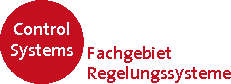
\includegraphics[width=1\textwidth]{Figures/csgLogo.pdf} 
%		\end{minipage}
%		\hfill
%		\begin{minipage}{0.12\textwidth}	
%		\end{minipage}
%		\hfill
%		% Logo Rechts
%		\begin{minipage}{0.23\textwidth}
%			\centering
%			
\includegraphics[width=0.9\textwidth]{Figures/tu-logo.eps} %[width=1.47in]{Bilder/tu-logo.eps} 
%		\end{minipage}
%		%\hfill
%		% Fakultät und Institut rechts
%		\begin{minipage}{0.30\textwidth}
%			\large \Fakultaet \vspace{1.5mm}  \\ Institut f\"ur Energie- und  \\Automatisierungstechnik%\Institut
%		\end{minipage} %\Large
%	\end{minipage}
%	
%	% Zwischenraum
%	\vspace{4.5cm} %3cm
%	
%	% Haupt- und Untertitel 
%	{\Huge \Titel}\\[7mm]
%	\begin{minipage}{11cm}
%		\centering \LARGE   \flqq  \Untertitel \frqq
%	\end{minipage}\\
%	
%	% Zwischenraum
%	\vspace{1cm}%2.5cm
%	
%	% Gruppen- bzw. Autorenangabe
%	{\small \Gruppe}\\[0.2cm]
%	\begin{tabular}{rl}
%		\Autor  & \AutorMatrikelNr  \\
%		\ifdefempty{\AutorB}{}{\AutorB & \AutorBMatrikelNr \\} 
%		\ifdefempty{\AutorC}{}{\AutorC & \AutorCMatrikelNr \\} 
%		\ifdefempty{\AutorD}{}{\AutorD & \AutorDMatrikelNr \\} 
%		\ifdefempty{\AutorE}{}{\AutorE & \AutorEMatrikelNr \\} 
%	\end{tabular}
%	
%	% Zwischenraum
%	\vspace{3.3cm}%2cm
%	
%	% Grad
%	\begin{minipage}{11cm}
%		\centering
%		A thesis submitted for the degree of\\[0.3cm]
%		{\LARGE \textbf{-- Master of Science --}}\\[0.3cm]
%		in Computational Engineering Science
%	\end{minipage}
%	
%	
%	% 2.Zwischenraum
%	\vspace{3.3cm}
%	
%	% Professoren und Betreuer
%	\begin{tabular}{ll}
%		Examiner: & \Professor \\[1mm]
%		Co-Examiner: & \ProfessorII \\[1mm]
%		\ifdefempty{\BetreuerA}{}{Supervisor:  & \BetreuerA \\ }
%		\ifdefempty{\BetreuerB}{}{  & \BetreuerB \\ }
%	\end{tabular}
%	
%	% Umbruch bei langen Titeln verhindern
%	\enlargethispage{1cm}
%	
%	% Zwischenraum
%	\vfill
%	
%	% Footer erstellen
%	\Uni, \Fakultaet{} -- \Institut, \\ \Fachgebiet \\ \Datum
%	
%\end{titlepage}






%% !TEX encoding = UTF-8 Unicode
%% !TEX spellcheck = de_DE
%% !TEX root = ../main.tex
%
\begin{titlepage}
	\begin{spacing}{2}
			
			\begin{flushright} %rechtsbündig (Anfang)
					\vspace*{-20mm}
					
\includegraphics[width=\textwidth]{Figures/title/CoverLogos.pdf}
					%
\includegraphics[width=\textwidth]{skizzen/CoverLogos_MZH}
				\end{flushright} %rechtsbündig (Anfang)
			
			% der Titel der Arbeit:
			\vspace{38mm} {\centering {{\LARGE{\Titel}}} % Alternativ: Titel hier manuell eingeben und mit "\\"den Zeilenumbruch schön machen
					
					\vfill
					% hier kommt eine hübsche Grafik hin:
					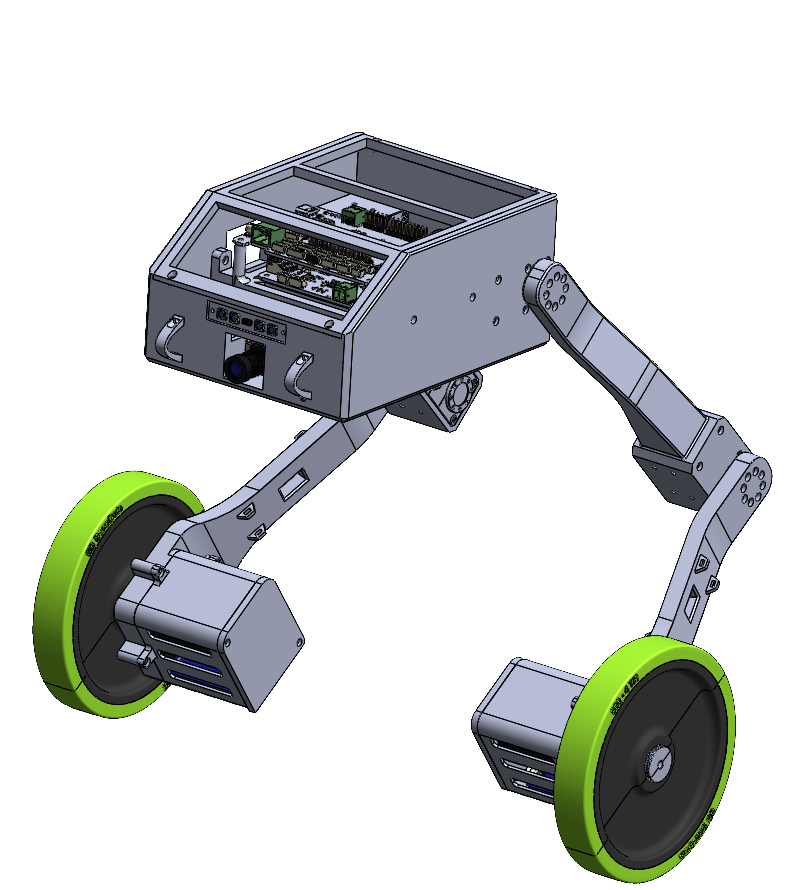
\includegraphics[width = 80mm]{Figures/title/Robot_Assembly_3}
					
					
					\vfill }
		\end{spacing}
	\begin{spacing}{1}
			\begin{tabular}{l}
					\Large{\ArtDerArbeit~\Kennnummer}
					% Die einzutragende Nummer gibt es beim Betreuer!
				\end{tabular}
			
			\vspace{5mm}
			
			\begin{tabular}{l}
					\large{\Autor}\\
					\large{Matrikelnummer \AutorMatrikelNr}
				\end{tabular}
			
			\vspace{5mm}
			
			\begin{tabular}{l}
					\large{Hannover, \Datum}
				\end{tabular}
			
			
			\vspace{5mm}
			{\large
					\begin{tabular}{l l}						
							First Examiner  & \Erstpruefer\\
							Second Examiner & \Zweitpruefer\\
							Supervisor    	& \Betreuer\\
						\end{tabular}
				}
			
		\end{spacing}
\end{titlepage}
%\cleardoublepage

%include Declaration of Authorship
% !TEX encoding = UTF-8 Unicode
% !TEX spellcheck = de_DE
% !TEX root = ../main.tex

\newpage
% Logos oben einbinden
\begin{flushright}
			\vspace*{-20mm}
			
\includegraphics[width=\textwidth]{Figures/title/CoverLogos.pdf}
\end{flushright}
	
\begingroup
\renewcommand{\cleardoublepage}{}
\renewcommand{\clearpage}{}
\chapter*{Declaration of Authorship}
\endgroup
\thispagestyle{empty}

%Kennnummer platzieren:
\begin{tikzpicture}[remember picture, overlay]
\node[xshift=-22mm,yshift=-43mm,anchor=north east,align=right] at (current page.north east){\Large{\textbf{\Kennnummer}}};
\end{tikzpicture}
%
%
\begin{tabular}{@{}p{0.25\textwidth} p{0.7\textwidth}}
\textbf{Name:} 		& \textbf{\Autor} \\ % Name des Autors
Registration no.: & \Matrikelnummer \\ % Matrikelnummer
\\
Thesis title: 		& \TitelDerArbeit \\
\\
Type of thesis: 	& \ArtDerArbeit\\
Study program: 		& International Mechatronics\\ %
%Mechanical Engineering\\ % Please Choose:
Submission date:	& \Datum \\
\\
First examiner : 	& \Erstpruefer\\
Second examiner: 	& \Zweitpruefer\\
Supervisor: 			& \Betreuer
\end{tabular}

\vspace{10mm}

I, \emph{\Autor}, hereby affirm that the \ArtDerArbeit~entitled \emph{\TitelDerArbeit}~was written independently, that no references and aids other than those indicated were used, that all passages of the thesis which were taken over literally or analogously from other sources are marked as such and that the thesis has not yet been presented to any examination board in the same or similar form.

I hereby agree to the transmission of my work also to external services for plagiarism checking by plagiarism software.

\vspace{5mm}


\noindent Hannover, \Datum



\vspace{20mm}
(\Autor)

%\end{spacing}
% Leerseite einfügen
\cleardoublepage

% If desired, include a blank page
\newpage
\thispagestyle{empty}
\mbox{}

% If desired, include a declaration of authorship
\chapter*{Eigenst\"andigkeitserkl\"arung}
\label{cha:Ehrenwort}
\thispagestyle{empty}
Hiermit erkl\"are ich, dass ich die vorliegende Arbeit selbstst\"andig und eigenh\"andig sowie ohne
unerlaubte fremde Hilfe und ausschlie\ss lich unter Verwendung der aufgef\"uhrten Quellen und
Hilfsmittel angefertigt habe.

\vspace{3cm}

\begin{tabular}{lp{4em}l}
 \hspace{4cm}   && \hspace{4cm} \\ \cline{1-1} \cline{3-3} \rule{0pt}{3.5ex} 
 Ort, Datum     && \Autor
\end{tabular}






% Include abstract

\selectlanguage{english}
\begin{abstract}
%General Problem
The robotic industry is growing rapidly.
Robots are becoming more and more capable and are used in a wide range of applications.
The design, modeling and control of robotic systems is a research field that is constantly evolving.

%% Research Gap
However, there are still many challenges to overcome.
The design of robotic systems is still a complex and time-consuming process, particularly in regard to multi-legged robots that should be able to execute complex maneuvers.
The control of robotic systems is still a challenging task, especially when it comes to dynamic and complex systems.
The search for the optimal control strategy is still an open research question.

%% Content
This thesis presents an in-depth exploration of the dynamic control and design of robotic systems.
The main focus is on the design and control of a multi-legged robot.
The robot is designed and built from scratch, including the mechanical and electronic design.
A combination of theoretical modeling and practical implementation were used to achieve the desired objectives.
The research first focuses on the design of a multi-legged robot that is capable of executing complex maneuvers. The robot is then modeled and simulated in a virtual environment.
The simulation is used to test and evaluate the robot's performance.
The robot is then built and tested in real life.
The research investigates the main elements that affect maneuverability and stability, such as the integration of multiple degrees of freedom, structural integrity, and weight distribution.


%% Contributions
Significant results are achieved in the design and control of the robot.
The robot demonstrates the capability to maintain balance while adjusting its hip and knee joint angles, as well as exhibits stable locomotion on its two wheels, effectively navigating within the simulated environment.
The robot's design is optimized to find the best trade-off between stability and maneuverability.
Different problems are addressed throughout the research, such as the design complexity to meet the mobility requirements, Incorporating the changing location of the center of mass in the dynamic model, and retuning the control of the robot when one or both of the joint angles change.
The developed Legged two-wheeled inverted pendulum robot serves as a platform for future research to build upon and test different control strategies.

%Furthermore
This research contributes valuable insights into the field of robotics, offering practical solutions for the challenges faced in designing and controlling wheeled and bipedal robots.
It lays a foundation for future innovations, aiming to broaden the scope and capabilities of robotic systems in real-world applications.




%Overall, this thesis provides a valuable contribution to the field of
%%%
\par
\keywords{Robotics, Multi-Legged Robot, Control, Simulation, Design, CAD, Modeling, Inverted Pendulum, Two-Wheeled bi-pedal legged robot}
\end{abstract}





% If desired, uncomment the table of contents
\tableofcontents

% From the Backmatter --
% If desired, uncomment the list of figures
\listoffigures

% If desired, uncomment the list of tables
\listoftables

% If desired, uncomment the list of listings
%\lstlistoflistings

% Include this switch if symbols, abbreviations, etc., without reference in the document should be included in the directories (usually the case)
% \glsaddall
%\glsaddallunused

%\setglossarypreamble[main]{This list of glossary entries only includes the most important items. Descriptions might not be universal and are intended for this thesis.}

%% If desired, uncomment the glossary (will only be created if entries are available)
%\setglossarystyle{long3col}
%%\setglossarystyle{long}
%\renewenvironment{theglossary}%
% {\begin{longtable}{lp{\glsdescwidth}p{\glspagelistwidth}}}
	% %{\begin{longtable}[l]{lp{\glsdescwidth+\glspagelistwidth+0cm}}}%
		% {\end{longtable}}
	%\renewcommand{\glsnamefont}[1]{\textbf{#1}}
	%\printglossary[type=main, style=altlist]%[style=index]
	%\glsfindwidesttoplevelname
	%\glssetwidest[1]{transfer error dynamics}
	%\setglossarystyle{alttree}
	%\printglossary[type=main]
	
	% If desired, uncomment the abbreviations (will only be created if entries are available)
	%\printglossary[type=\acronymtype, nonumberlist]%[type=\acronymtype,style=list]
	
	% If desired, uncomment the symbols (will only be created if entries are available)
	%\printglossary[type=symbols, style=symb3spaltig, nonumberlist]
	%\printglossary[type=symbols, nonumberlist]
	
	%\chanumfalse
\addchap{Notation} % add chapter without numbering that appears in table of contents
% Manuelles Symbolverzeichnis
% ___________________________________________________________________
% ============================ NOTATION ==========================
% ====================================================================
\begin{table}[h]
	\renewcommand{\arraystretch}{1.4}
	\begin{tabularx}{1\textwidth}{@{}lX@{}}
		\toprule
		\textbf{Example} & \textbf{Description}  \\ \midrule
		$\mathbb{R}, \mathbb{N}$ 	& Capital letters in blackboard bold font represent common number types. \\
		$\mathcal{A}, \mathcal{T}$ 	& Capital letters in calligraphic font represent custom sets or its members. \\
		$\vec{A}, \vec{P}$ 			& Capital bold letters represent matrices.	\\
		$\vec{x}, \vec{f}$			& Lower-case bold letters represent column vectors or vector-functions. \\
		$F(z), T(s)$				& Capital regular letters represent transfer functions.	\\		
		$i, e^{(i \rightarrow j)}$	& Lower-case regular letters represent scalars and scalar-functions.\\
		$\vec{x}^{(i)}, F^{(2)}$	
			& A single upper, bracketed index represents the dependency on a single, specific agent.\\
		$ H^{(1, 2)}, e^{(i, j)}$ 
			& Two upper, bracketed indices represent the dependency on two specific agents, where the order of the agents is not relevant.\\
		$ H^{(1 \rightarrow 2)}, e^{(i \rightarrow j)}$
			& An arrow between two upper, bracketed indices represent the directional dependency on two specific agents, where the order of the agents matters.\\
		$\hat{\vec{t}}^{(i \rightarrow j)}, \hat{\mathbf{P}}^{(1)}$ 
	     	& An upper hat symbol represents an estimated or approximated entity.\\	
		$\bar H^{(1 \rightarrow 2)}, \bar e^{(i \rightarrow j)}$
	     	& An upper bar symbol represents a mean value.\\	
		\bottomrule
	\end{tabularx}
	\caption[General notation style]{General notation style. Some exceptions are possible.}
\end{table}

% ====================================================================
\begin{notebox}
	To be precise, the error dynamics depend on the order of agent $i$ and $j$, 
	since they differ in their sign.
		\begin{equation}
			H^{(i,j)}\neq H^{(j,i)}
		\end{equation}			
		However, both result in the same \gls*{output_error}. 
		$H^{(i,j)}$ and $H^{(j,i)}$ are not distinguished in this work, 
		which is consistent with the given notation. This also applies to other cases like the error trajectory $\vec{e}^{(i,j)}$ or the output error $\varepsilon^{(i,j)}_{\vec{u}}$ as well.
\end{notebox}

% ====================================================================
\pagebreak
\renewcommand{\arraystretch}{1.3}
\begin{tabularx}{1\textwidth}{@{}lX@{}}
    \endfirsthead \endhead \endfoot \endlastfoot
    \toprule
	\multicolumn{2}{@{}l}{\textbf{Mathematical Notations}} \\ 
	\textit{Symbol} & \textit{Description}  \\ \midrule
	$\left\Vert \cdot \right\Vert_2$ & denotes the 2-norm \\
	$\left\Vert \cdot \right\Vert_{\infty}$ & denotes the maximum-norm \\
	$ |\cdot |$	& 
	\begin{enumerate*}[label=(\roman*)]
		\item absolute of a number or 
		\item gain of a transfer function
	\end{enumerate*} \\
	$\angle $ & denotes the phase of a transfer function \\
	$\circ$	& denotes the composition of two functions or matrices \\
	$\vec{0}$ & denotes a zero vector or zero matrix  \\
	$\vec{I}$ & denotes the unit matrix \\
%		$\emptyset$ & denotes an empty set\\
	$\mathcal{N}(\mu, \sigma^2)$& normal distribution with mean $\mu$ and standard deviation $\sigma$ \\ 
	\bottomrule
	\multicolumn{2}{@{}l}{\textbf{General Parameters}} \\ 
	\textit{Symbol} & \textit{Description}  \\ \midrule
	$k, l$		 				&  running indeces \\
	$t$							&  time or duration (in seconds) \\
	$n_{\mathcal{A}}$	 		&  number of agents in a MAS \\
	$N, R$				 		&  dimension of a vector, matrix, i.e. length of an input trajectory \\
	$K$					 		&  degree of a biproper transfer function \\
	$K_N, K_D$		 	 		&	degree of numerator, denominator of a transfer function \\
	$m$						 	&  relative degree of a dynamic system \\
	$f_s, f_\mathrm{cutoff}, f$	&  sample frequency, cutoff frequency, other frequencies in $1/\unit{s}$\\ 
	\bottomrule
	\multicolumn{2}{@{}l}{\textbf{Sets \& Agents}} \\ 
	\textit{Symbol} & \textit{Description}  \\ \midrule
	$i, j$				 &  indices of a specific, but arbitrary agent in a MAS \\
	$\mathbb{R}$		 &	set of all real numbers \\
	$\mathbb{R}^n$		 &	$n$-dimensional set of all real numbers \\
	$\mathbb{N}_0$		 &  set of all natural numbers and zero \\
	$\mathcal{U}^{(i)}$	 	&  input space of agent $i$ \\
	$(\mathcal{U}^{(i)})^N$ &  input space of agent $i$ for input sequences of length $N$\\
	$(\mathcal{U}^{(i,j)})^N$&  input space of agent $i$ and $j$ for input sequences of length $N$ with 
	$(\mathcal{U}^{(i)})^N \cap (\mathcal{U}^{(j)})^N$ \\
    $\mathcal{A}$    	 &  set of all agents in a MAS\\
    $\mathcal{A}^{(i)}$  &  specific agent with index $i$\\
    $\mathcal{T}$    	 &  set of input maps between all agents in a MAS \\
    \bottomrule\\[10mm]\\[0.01mm]    
	\toprule
	\multicolumn{2}{@{}l}{\textbf{Discrete time step $k$}} \\ 
	\textit{Symbol} & \textit{Description}  \\ \midrule
	$k$			 &  time (sample) index for discrete systems and trajectories \\	    
    $u_{k}$		 & scalar input at time step $k$ \\
    $y_{k}$		 & scalar output at time step $k$ \\
   		$e^{(i,j)}_{k}$		 	 
   			& difference $y^{(j)}_k-y^{(j)}_k$ between the outputs of agent $i$ and $j$ at time $k$\\
   		$w_k$
   			& noise drawn from a normal distribution with zero mean and variance $\sigma^2$\\
    $\vec{x}^{(i)}_{k}$  & state of agent $i$ at time $k$ \\	
	$\vec{\tilde{f}}$ 	
		& state-function that advances the state $\vec{x}$ one step in time \\
	$\tilde{h}$ 	
		& output-function that returns the current output depending on the 
		current state and input\\   
	$\vec{A}, \vec{B}, \vec{C}$ 
		& state matrix, input matrix, output matrix of a linear system in discrete-time 
		state-space representation \\ \bottomrule
	\multicolumn{2}{@{}l}{\textbf{Transfer Function Representation}} \\ 
	\textit{Symbol} & \textit{Description}  \\ \midrule
	$s, z$ & denotes a transfer function in continuous time, discrete time\\
	$U(s), U(z)$		
		& System input in $s$-domain, $z$-domain\\
	$E(s), E(z)$		
		& $s$-Transformation, $z$-Transformation of the difference $y^{(j)}-y^{(j)}$\\
	$F$				
		& Transfer function of of a linear system\\
	$F^{(i\rightarrow j)}$	
		& \Glsc{deviation_system} in the transfer-function representation from agent $i$ to agent $j$	\\
	$Q$	
		& Filter function\\	
	$\hat{T}^{(i\rightarrow j)}$	
		& Estimation of the \glsc{input_map} in the transfer-function representation from agent $i$ to agent $j$\\
	$H^{(i,j)}$	
		& \Glsc{error_dynamics} in the transfer function representation describing the difference between agent 
		$i$ and $j$ when the same input is applied to both systems\\
	$H^{(i \rightarrow j)}$	
		& \Glsc{transfer_error_dynamics} in the transfer function representation describing the difference between agent 
		$i$ and $j$ including the input-transfer $\hat T^{(i \rightarrow j)}$\\	
	$a_k, b_k$ & Numerator, denominator coefficients in transfer-function \\ \bottomrule%\\[54mm]\\[0.01mm] \toprule
	\multicolumn{2}{@{}l}{\textbf{Batch Process \& Lifted System Representation}} \\ 
	\textit{Symbol} & \textit{Description}  \\ \midrule
	$\vec{u}, \vec{v}$		  	
		& An \glsc{input_trajectory} as a sequence of scalar inputs of length $N$\\
	$\vec{\tilde u}^{(i)}$	
		& Input trajectory of length $N$ for agent $i$ that results from some input-transfer 
		$\vec{t}^{(j\rightarrow i)}$\\
	$\vec{y}$		 	
		& An \glsc{output_trajectory} as a sequence of scalar outputs of length $N$\\
	$\vec{e}^{(i,j)}$
		& An \glsc{error_trajectory} describing the difference $\vec{y}^{(j)}-\vec{y}^{(i)}$ between the 
		output trajectories of agent $i$ and $j$\\
	$\vec{e}^{(i\rightarrow j)}_{\vec{u}}$
		& \Glsc{transfer_error_trajectory} describing the difference $\vec{y}^{(j)}-\vec{y}^{(i)}$ between the 
		output trajectories of agent $i$ and $j$ for a certain input trajectory $\vec{u}$\\ \midrule\\[0.1mm] \midrule
	\textit{Symbol} & \textit{Description}  \\ \midrule	
	$\vec{w}$
		& Sequence of normally distributed noise values with zero mean and variance $\sigma^2$\\ 	
	$\vec{f}$ 			
		& Nonlinear \glsc{batch_function} that maps a given input trajectory to a corresponding 
		output trajectory \\
	$\vec{f}^{(i\rightarrow j)}$
		& \Glsc{deviation_system} as a \gls*{batch_function} from agent $i$ to agent $j$\\
	$\mathbf{t}^{(i\rightarrow j)}$	
		& \Glsc{input_map} as a \gls*{batch_function} from agent $i$ to agent $j$\\
	$\mathbf{\hat t}^{(i\rightarrow j)}$	
		& Estimated input-transfer batch-function from agent $i$ to agent $j$
		(Here as a general expression for either $\mathbf{\hat T}^{(i\rightarrow j)}$ or $T^{(i\rightarrow j)}$)\\
	$\mathbf{h}^{(i\rightarrow j)}$	
		& \Glsc{error_dynamics} as a \gls*{batch_function} describing the difference between agent 
		$i$ and $j$ when the same input is applied to both systems.\\
	$\vec{P}$				
		& lifted-system matrix that maps an input trajectory to an output trajectory\\
	$\vec{P}^{(i\rightarrow j)}$	
		& \Glsc{deviation_system} in the lifted-system representation from agent $i$ to agent $j$\\
	$\mathbf{T}^{(i\rightarrow j)}$	
		& \Glsc{input_map} in the lifted-system representation from agent $i$ to agent $j$\\
	$p_k, p^{(i \rightarrow j)}_k$					
		& $k$-th parameter in lifted-system matrix $\vec{P}, \vec{P}^{(i\rightarrow j)}$\\
	$t^{(i\rightarrow j)}_k$	
		&  $k$-th parameter in lifted-system matrix $\mathbf{T}^{(i\rightarrow j)}$\\ \bottomrule
	\multicolumn{2}{@{}l}{\textbf{Error Metrics}} \\ 
	\textit{Symbol} & \textit{Description}  \\ \midrule
   		$\varepsilon^{(i,j)}$ % \left(\vec{y}^{(i)}, \vec{y}^{(j)}\right)	 	 
   			& \Glsc{output_error}: 2-norm of the difference between the output trajectories of agent $i$ and $j$\\	
   		$\varepsilon^{(i,j)}_{\vec{u}}$ %\left(\vec{u}^{(i)}\right)		 	 
   			& \Glsc{direct_transfer_error}: Output error $e^{(i,j)}$ when the same input is applied 
   			to agents $i$ and $j$ \\
	$\varepsilon^{(i\rightarrow j)}_{\vec{u}}$ 
		& \Glsc{transfer_error}: Output error $\varepsilon^{(i,j)}$  for a certain input trajectory $\vec{u}$ 
			after applying the \gls*{input_map} $\vec{t}^{(i \rightarrow j)}$ to agent $j$ \\	
	$\varepsilon^{(i\rightarrow j)}_{\vec{u},\mathrm{NRMS}}$ 
		& \Glsc{nte}: Transfer error $\varepsilon^{(i\rightarrow j)}_{\vec{u}}$ 
		normalized to the \gls*{direct_transfer_error} $\varepsilon^{(i,j)}_{\vec{u}}$\\	
	\bottomrule
	\caption{Mathematical notations}
\end{tabularx}

\chanumtrue
    
	% --
	
	% Save page number for Back Matter and conclude Front Matter
\newcounter{RomanNumbers}
\addtocounter{RomanNumbers}{\value{page}}
\clearpage

%
%% Body Matter - Here the text of the document, the content, is set
% Page numbers of the content in Arabic numerals
\pagenumbering{arabic}

% Content

% Inserting the files, e.g.:
%\chapter{Introduction}

\graphicspath{{./Figures/Introduction/}}



\section{Motivation}
%This section should explore the underlying reasons for undertaking the research. It might include the importance of the topic, the gap in current knowledge, and the potential applications of the research findings.
%figure for Handle Boston Dynamics Robot
\begin {figure}[h]
\centering
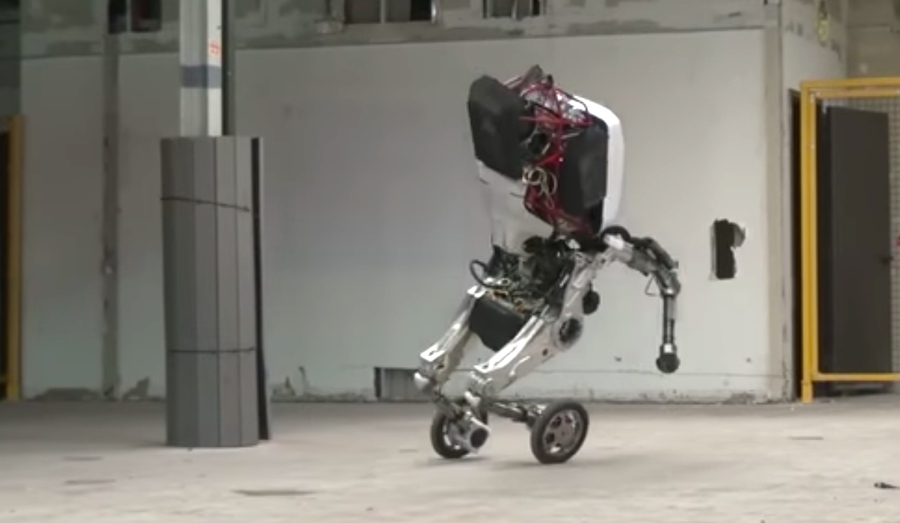
\includegraphics[width=0.7\textwidth]{boston-dynamics-handle-robot}
\caption{Handle Robot by Boston Dynamics\cite{handle}}
\label{fig:Handle}
\end {figure}


Robotics has always been a cutting-edge field that combines sophisticated engineering, artificial intelligence, and a comprehension of human-environment interactions.
This study is motivated by multiple important elements, all of which highlight the importance and relevance of the research.
The reasons for undertaking this research is the desire to advance the field of robotics, fill existing knowledge gaps, have a broad societal impact, and foster interdisciplinary collaboration.
By developing a multi-legged robotic system with enhanced movement capabilities and control strategies, this research endeavors to set new standards in robotic design and functionality. Even with significant advancements, there are still many unanswered questions about robotic control and locomotion, particularly in systems that replicate biological structures and processes. Complex dynamic tasks that living beings handle with ease are sometimes difficult for traditional robotic systems to accomplish. This research aims to close these gaps by concentrating on a multi-legged robot that finds inspiration in the natural environment. This will provide insights into more realistic and effective movement tactics. The applications of such advanced robotic systems are vast and varied, ranging from search and rescue operations in hazardous environments to assistive technology in warehouse automation.By pushing the boundaries of what is currently possible in robotic design and control, this research has the potential to make significant contributions to fields where human intervention is limited, dangerous, or impractical. This project is inherently interdisciplinary, integrating concepts from mechanical engineering, computer science, control theory, and even biology. Such cross-disciplinary collaboration is crucial for driving innovation, as it allows for the exchange of ideas and methods from diverse fields. This approach is expected to yield novel solutions and advancements that could extend well beyond the scope of this project.

%\textbf{Advancements in Robotic Technologies:}% Robotics has grown at an exponential rate over the past few decades, resulting in improved capabilities and more applications. Previously limited to industrial settings, robots are now being deployed in increasingly dynamic and unpredictable circumstances. The development of robotic systems that are more flexible, nimble, and intelligent is required due to this evolution. Our research is to create a sophisticated multi-legged robotic system that can perform intricate movements and interact with its surroundings.

%\textbf{Filling Knowledge Gaps:} %Even with significant advancements, there are still many unanswered questions about robotic control and locomotion, particularly in systems that replicate biological structures and processes. Complex dynamic tasks that living beings handle with ease are sometimes difficult for traditional robotic systems to accomplish. This research aims to close these gaps by concentrating on a multi-legged robot that finds inspiration in the natural environment. This will provide insights into more realistic and effective movement tactics.

%\textbf{Potential for Broad Impact:} %The applications of such advanced robotic systems are vast and varied, ranging from search and rescue operations in hazardous environments to assistive technology in healthcare. By pushing the boundaries of what is currently possible in robotic design and control, this research has the potential to make significant contributions to fields where human intervention is limited, dangerous, or impractical.

%\textbf{Interdisciplinary Collaboration and Innovation:} %This project is inherently interdisciplinary, integrating concepts from mechanical engineering, computer science, control theory, and even biology. Such cross-disciplinary collaboration is crucial for driving innovation, as it allows for the exchange of ideas and methods from diverse fields. This approach is expected to yield novel solutions and advancements that could extend well beyond the scope of this project.

%In summary, the motivation for this project lies in its potential to advance the field of robotics, fill existing knowledge gaps, have a broad societal impact, and foster interdisciplinary collaboration. By developing a multi-legged robotic system with enhanced movement capabilities and control strategies, this research endeavors to set new standards in robotic design and functionality.

\section{Explanation of the Goals and Requirements}
In this research, we aim to develop a multi-legged robotic system that can perform complex movements and interact with its environment.
The robot will be able to balance on two wheeled multi-jointed legs.
The robot would be based on the previous TWIPR robot.
Extra degrees of freedom will be added to the robot to allow for more complex movement.
The robot would be designed from scratch to meet the requirements of the project.
The robot would be designed using CAD software.
The design would take into account the mechanical, electrical, and software requirements of the robot.
Fabrication of the robot chassis would be done using 3D printing.Electrical design and assembly would be done using off-the-shelf components.
Mathematical modeling and simulation of the robot would be done to determine the robot's dynamics and control.
Different control strategies would be explored and implemented.
Development of firmware and software for the robot would be done.
The robot would be tested and evaluated in simulation and in real life.
The robot would be tested for its ability to balance and move in different environments. The robot would be tested for its ability to perform complex movements and interact with its environment.

%\include{Content/Chapter1}
%\include{Content/Conclusion}

% Then insert chapters in the files.
% % % % % % % % % % % % % % % % % % % % % % % % % % % % % % % % % % % % % % % % % % % % % % %
\chapter{Introduction}

\graphicspath{{./Figures/Introduction/}}



\section{Motivation}
%This section should explore the underlying reasons for undertaking the research. It might include the importance of the topic, the gap in current knowledge, and the potential applications of the research findings.
%figure for Handle Boston Dynamics Robot
\begin {figure}[h]
\centering
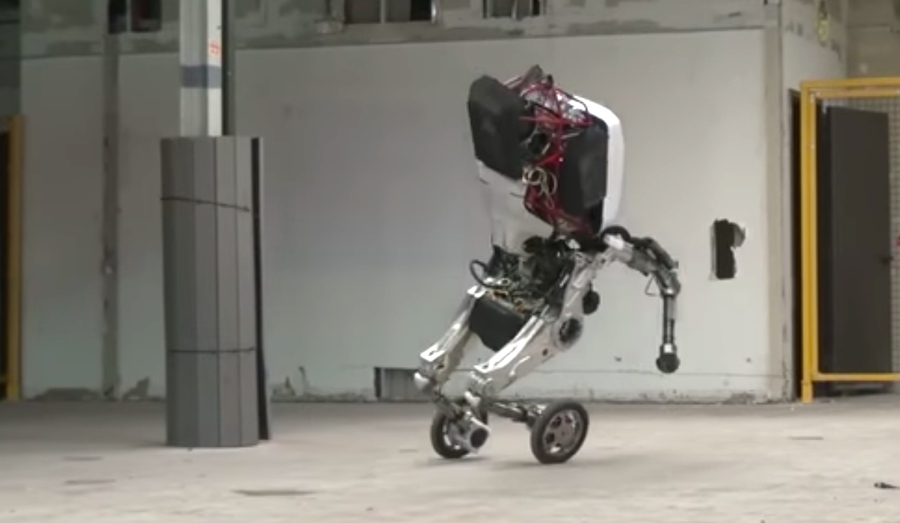
\includegraphics[width=0.7\textwidth]{boston-dynamics-handle-robot}
\caption{Handle Robot by Boston Dynamics\cite{handle}}
\label{fig:Handle}
\end {figure}


Robotics has always been a cutting-edge field that combines sophisticated engineering, artificial intelligence, and a comprehension of human-environment interactions.
This study is motivated by multiple important elements, all of which highlight the importance and relevance of the research.
The reasons for undertaking this research is the desire to advance the field of robotics, fill existing knowledge gaps, have a broad societal impact, and foster interdisciplinary collaboration.
By developing a multi-legged robotic system with enhanced movement capabilities and control strategies, this research endeavors to set new standards in robotic design and functionality. Even with significant advancements, there are still many unanswered questions about robotic control and locomotion, particularly in systems that replicate biological structures and processes. Complex dynamic tasks that living beings handle with ease are sometimes difficult for traditional robotic systems to accomplish. This research aims to close these gaps by concentrating on a multi-legged robot that finds inspiration in the natural environment. This will provide insights into more realistic and effective movement tactics. The applications of such advanced robotic systems are vast and varied, ranging from search and rescue operations in hazardous environments to assistive technology in warehouse automation.By pushing the boundaries of what is currently possible in robotic design and control, this research has the potential to make significant contributions to fields where human intervention is limited, dangerous, or impractical. This project is inherently interdisciplinary, integrating concepts from mechanical engineering, computer science, control theory, and even biology. Such cross-disciplinary collaboration is crucial for driving innovation, as it allows for the exchange of ideas and methods from diverse fields. This approach is expected to yield novel solutions and advancements that could extend well beyond the scope of this project.

%\textbf{Advancements in Robotic Technologies:}% Robotics has grown at an exponential rate over the past few decades, resulting in improved capabilities and more applications. Previously limited to industrial settings, robots are now being deployed in increasingly dynamic and unpredictable circumstances. The development of robotic systems that are more flexible, nimble, and intelligent is required due to this evolution. Our research is to create a sophisticated multi-legged robotic system that can perform intricate movements and interact with its surroundings.

%\textbf{Filling Knowledge Gaps:} %Even with significant advancements, there are still many unanswered questions about robotic control and locomotion, particularly in systems that replicate biological structures and processes. Complex dynamic tasks that living beings handle with ease are sometimes difficult for traditional robotic systems to accomplish. This research aims to close these gaps by concentrating on a multi-legged robot that finds inspiration in the natural environment. This will provide insights into more realistic and effective movement tactics.

%\textbf{Potential for Broad Impact:} %The applications of such advanced robotic systems are vast and varied, ranging from search and rescue operations in hazardous environments to assistive technology in healthcare. By pushing the boundaries of what is currently possible in robotic design and control, this research has the potential to make significant contributions to fields where human intervention is limited, dangerous, or impractical.

%\textbf{Interdisciplinary Collaboration and Innovation:} %This project is inherently interdisciplinary, integrating concepts from mechanical engineering, computer science, control theory, and even biology. Such cross-disciplinary collaboration is crucial for driving innovation, as it allows for the exchange of ideas and methods from diverse fields. This approach is expected to yield novel solutions and advancements that could extend well beyond the scope of this project.

%In summary, the motivation for this project lies in its potential to advance the field of robotics, fill existing knowledge gaps, have a broad societal impact, and foster interdisciplinary collaboration. By developing a multi-legged robotic system with enhanced movement capabilities and control strategies, this research endeavors to set new standards in robotic design and functionality.

\section{Explanation of the Goals and Requirements}
In this research, we aim to develop a multi-legged robotic system that can perform complex movements and interact with its environment.
The robot will be able to balance on two wheeled multi-jointed legs.
The robot would be based on the previous TWIPR robot.
Extra degrees of freedom will be added to the robot to allow for more complex movement.
The robot would be designed from scratch to meet the requirements of the project.
The robot would be designed using CAD software.
The design would take into account the mechanical, electrical, and software requirements of the robot.
Fabrication of the robot chassis would be done using 3D printing.Electrical design and assembly would be done using off-the-shelf components.
Mathematical modeling and simulation of the robot would be done to determine the robot's dynamics and control.
Different control strategies would be explored and implemented.
Development of firmware and software for the robot would be done.
The robot would be tested and evaluated in simulation and in real life.
The robot would be tested for its ability to balance and move in different environments. The robot would be tested for its ability to perform complex movements and interact with its environment.

\chapter{Table of content Draft }

\graphicspath{{./Figures/Modeling}}

Questions to answer in each section 


\begin{enumerate}
	\item what is going to be in here?
	\item how long or how elaborate?
	\item what is the purpose (the take home message)? 
\end{enumerate}






\begin{enumerate}
	\item Introduction
	\begin{enumerate}
		\item Background and Motivation
		\begin{enumerate}
			\item Discuss the evolution and significance of robotics in various industries.
			\item Emphasize the need for advancements in robotic stability and mobility.
		\end{enumerate}

		\item Problem Statement
		\begin{enumerate}
			\item Define the specific challenges in designing a legged self-balancing robot.
		\end{enumerate}
		\item Objectives(Outline the primary goals of the thesis)
	\end{enumerate}
	\item Literature Review
	\begin{enumerate}
		\item Overview of Robotics
		\item Previous Work in Self-Balancing Robots
		\item Control Strategies 
		\begin{enumerate}
			\item what is going to be in here? a comparison of the control strategies used.
			\item how long or how elaborate? not too detailed but with more explanation of the control theory used in the project
			\item what is the purpose (the take home message)? pros and cons of the different and why would we prefer one of them over the other depending on the applications
		\end{enumerate}
	\end{enumerate}
	\item Design and Development of the Robot
	\begin{enumerate}
		\item Mechanical Design
		\begin{enumerate}
			\item Initial calculations 
			\begin{enumerate}
				\item what is going to be in here? -> torque initial calculations
				\item how long or how elaborate? -> two or three scenarios
				\item what is the purpose (the take home message)? for choosing the correct motors 
			\end{enumerate}
			\item design 
		\begin{enumerate}
				\item what is going to be in here?-> CAD design and the explanations of the challenges 
				\item how long or how elaborate? detailed explanations of the reason behind the design decision
				\item what is the purpose (the take home message)? assembling the robot with fitting parts to match the new model requirements  
			\end{enumerate}
			\item Modeling 
			\begin{enumerate}
				\item what is going to be in here?-> the figures for the new model and the new COG and MOI calculations and the equations of motion.  
				\item how long or how elaborate? 4 to 5 pages explaining the equations in details 
				\item what is the purpose (the take home message)? showing the calculations for the new model and it would influence the equations of motion.
			\end{enumerate}
		\end{enumerate}
		\item Electrical Design
		\begin{enumerate}
			\item what is going to be in here? Component diagram showing the choice of all the components and there intended use and why we chose each of these components 
			\item how long or how elaborate? detailed explanation of the  requirement boards for operating the robot, the choice of components based calculations for the motors.
			\item what is the purpose (the take home message)? show how the Electrical design is configured in the optimal way to operate the robot 
		\end{enumerate}
		\item Software and Control
		\begin{enumerate}
			\item Control Algorithm 
			\begin{enumerate}
				\item what is going to be in here?->flowchart of the Control Algorithm
				\item how long or how elaborate?-> detailed explanation of the used control theory 
				\item what is the purpose (the take home message)? -> how the control is implemented 
			\end{enumerate}
			\item Firmware
		\end{enumerate}
		\item Safety 
		\begin{enumerate}
			\item what is going to be in here? different design changes for safety measures(motors covers, wire routing, body bumper, distance sensor , algorithm safety, electrical safety )
			\item how long or how elaborate? 1 or two pages max that include the 
			\item what is the purpose (the take home message)? the safety measures taken to minimize crashes, failure
		\end{enumerate}
	\end{enumerate}
	\item Experimental Setup and Methodology
	\begin{enumerate}
		\item Simulation Environment
		\item Physical Prototype Testing
		\item Data Collection and Analysis
	\end{enumerate}
	\item Results and Discussion
	\begin{enumerate}
		\item Simulation Results
		\item Real-world Performance
		\item Comparison and Analysis
	\end{enumerate}
	\item Conclusion and Future Work
	\begin{enumerate}
		\item Summary of Findings
		\item Contributions
		\item Recommendations for Future Research
	\end{enumerate}
\end{enumerate}

\chapter{Mechanical Design}

\graphicspath{{./Figures/Mechanical Design/}}



	
%	\item Outline the purpose and scope of the chapter.

 Modeling In this chapter, the details of the mechanical design are presented. where it goes from the initial conceptual design to the final design showing in the process the design decision-making for each critical point, This chapter emphasis the detailed description of the precise placement and alignment of different components such as the motors, wheels, battery, boards, and others to maintain the seamless integration of all the components into the robot body.
%	\item Briefly describe the mechanical design's role in the overall project.
\newline
The mechanical design serves as an important pillar to define the new physical form, size, and shape of the TWIPR. Depending on how these criteria are defined, the robot would interact with the environment. taking into account that the design directly influences the center of gravity, which is crucial to consider in our robot due to the inverted pendulum nature to be able to balance and maintain the upright position. In addition to the impact that the design has on the maneuverability of the robot and how it would respond to the control signals to be able to execute a task.

\newpage


\section{Design Objectives and Requirements}

%	Detail the primary objectives of the mechanical design
	The main objective is to come up with a new design for a multiple joints Robot to perform complex dynamic movements. this robot would be based on the Two wheeled inverted pendulum robot. The new design would add more degrees of freedom to enable the more complex movements.This enhances the robot capabilities where it can execute more diverse scenarios. 
%	\item List the requirements that the design must meet (e.g., weight limits, size constraints, mobility requirements).
	Initially, the main requirement was to add more two degrees of freedom where originally it used to have one degree of freedom in the wheels. The new design has three degrees of freedom one in the wheels, one as a knee joint and one as a hip joint. The current design has two identical legs.

\section{Conceptual Design}
%Discuss the initial design concepts.
As for the initial design concepts the body was that main point of focus as shown in the figure.Three initial designs where considered mainly for the body.\ Symmetrical vertical body in figure A, symmetrical horizontal body in figure B and leaning forward body in figure C.
\ For the three designs, two independent legs where considered.
two designs where considered for the legs, the normal joint leg and the compliant leg
% figure of the initial design concepts
\begin{figure}[h]
	\centering
	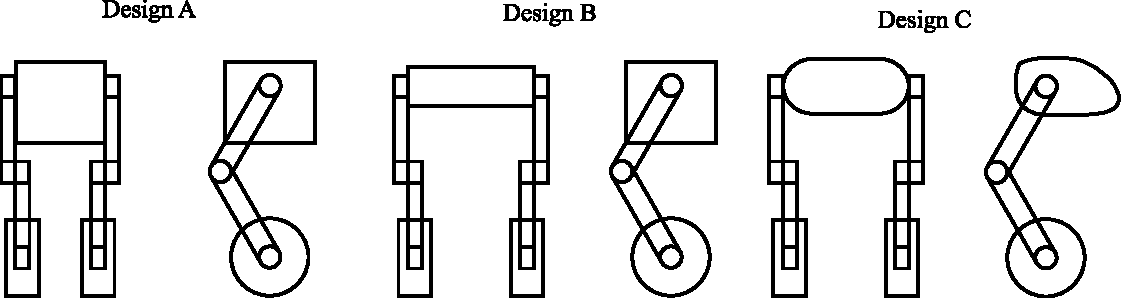
\includegraphics[width=1\linewidth]{Conceptual Design}
	%\includegraphics[width=0.5\linewidth]{Figures/Mechanical Design/Conceptual_Design}
	\caption{Initial Design Concepts}
	\label{fig:initialdesigns}
\end{figure}

the compliant leg is more flexible and can be used to absorb the shock from the ground.\ The normal joint leg is more rigid and can be used to generate more torque.in addition, the normal is more relative to our use-case as it can precisely control the position of the leg.
% figure for the leg designs
\begin{figure}[h]
	\centering
	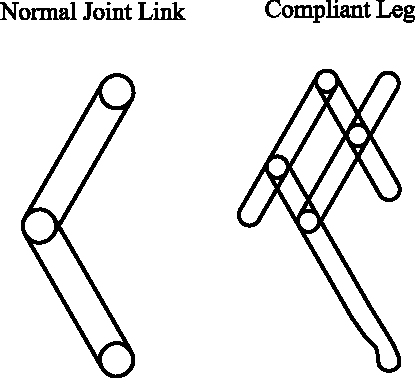
\includegraphics[width=0.4\linewidth]{Leg Design}
	%\includegraphics[width=0.5\linewidth]{Figures/Mechanical Design/Conceptual_Design}
	\caption{Leg Designs}
	\label{fig:legdesigns}
\end{figure}




%Explain the decision-making process for selecting the final concept.
% Include sketches or early design models.

\section{Detailed Design Development}
\begin{itemize}
	\item Elaborate on the development of the detailed mechanical design.
	\item Discuss material selection and the rationale behind these choices.
	\item Include detailed CAD drawings and design schematics.
\end{itemize}
\section{Design for Manufacturability and Assembly}
\begin{itemize}
	\item Discuss how the design facilitates manufacturing and assembly..
	\item Explain any design choices made to simplify these processes of manufacturing and assembly.
\end{itemize}
\section{Prototyping and Iterative Design}
\begin{itemize}
	\item Discuss the process of prototyping.
	\item Explain how feedback from prototyping phases was incorporated into design revisions.
\end{itemize}


\chapter{Electronic Design}

\graphicspath{{./Figures/Electronic Design/}}
In this chapter, the details of the electronic design are presented.
Where it emphasizes the details of the components' technical specifications and the selection process.
In addition to the wiring tree of the electronic components and the PCB design,
The chapter also discusses the power management.


\begin{itemize}
	\item Overview of the chapter's focus.
	\item Emphasize the importance of electronic design in the context of the overall project.
\end{itemize}


\section{Design Objectives and Constraints}
\begin{itemize}
	\item Clearly define the objectives and goals for the electronic design
	\item Discuss any constraints such as power requirements, size limitations.
\end{itemize}
\section{Component Selection}
The component diagram is shown in figure \ref{fig:componentsdiagram} shows the different components and their relationship with each other.
The main components are the microcontroller, rassberry pi, the motors, Distance sensor, Camera, the battery.
%figure of the components digram
\begin{figure}[h]
	\centering
	\includegraphics[width=1\linewidth]{Component_Diagram}
	%\includegraphics[width=0.5\linewidth]{Figures/Mechanical Design/Conceptual_Design}
	\caption[Components Diagram]{Components Diagram and there realationship with each other}
	\label{fig:componentsdiagram}
\end{figure}
\subsection{Hip and Knee Motors
%Details the selection process for key electronic components like microcontrollers,sensors, actuators, power supplies, etc.
The DYNAMIXEL XM430-W350 is chosen as a motor for the hip joint and the knee joint. The motor is chosen because it has a high torque to weight ratio and it has a high resolution of 4096 steps per revolution. The motor has a built-in driver and it can be controlled using a serial communication protocol. The motor has a built-in encoder that can be used to measure the position of the motor. The motor has a maximum torque of 3.5 Nm and a maximum speed of 46 RPM. The motor has a maximum current of 2.1 A and a maximum voltage of 12 V. The motor has a weight of 82 g and a size of 28.5 x 46.5 x 34 mm.
%figure of the DYNAMIXEL XM430-W350 motor
\begin{figure}[h]
	\centering
	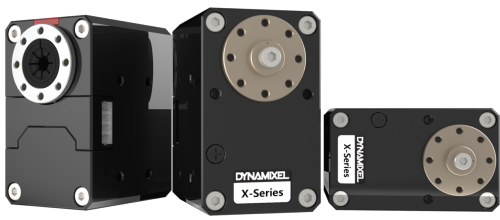
\includegraphics[width=0.5\linewidth]{DYNAMIXEL_XM430-W350}
	%\includegraphics[width=0.5\linewidth]{Figures/Mechanical Design/Conceptual_Design}
	\caption[DYNAMIXEL XM430-W350]{DYNAMIXEL XM430-W350}
	\label{fig:DYNAMIXEL_XM430-W350}
\end{figure}
%from the info on the website for SIMPLEX MOTION SC040A
%Continuous output of 120W and 280 mNm torque at 4000rpm
%Brushless outer rotor motor with peak torque of 800 mNm
%Integrated drive electronics with 4096 positions/revolution position sensor
%PID regulator for position or speed control with torque limit
%Ramp control of speed or position
%Protection features for current, torque, voltage and temperature
%Serial interface RS485 with Modbus RTU protocol
%CANOpen 301 interface
%Quadrature encoder input for application use
%Interface signals for step motor emulation (step/direction)
%Up to 8 digital inputs and 4 analog inputs
%4 digital outputs capable of 30V/1A, with pulse, PWM and RC Servo control modes.
%PC based software for setup and testing

The SIMPLEX MOTION SC040A is chosen as a motor for the wheels. The motor is chosen since it has a output of 120W and 280 mNm torque at 4000rpm. The motor has a built-in driver and it can be controlled using RS485 serial communication protocol. The motor has  position and speed control with torque limit. The motor has a maximum torque of 800 mNm.
%figure of the SIMPLEX MOTION SC040A motor
\begin{figure}[h]
	\centering
	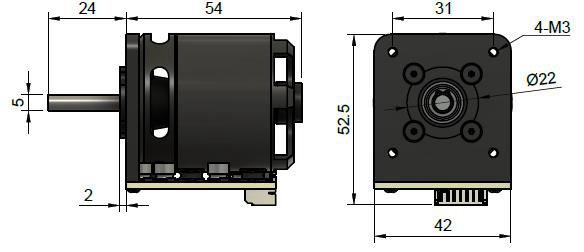
\includegraphics[width=0.5\linewidth]{SIMPLEX_MOTION_SC040A}
	%\includegraphics[width=0.5\linewidth]{Figures/Mechanical Design/Conceptual_Design}
	\caption[SIMPLEX MOTION SC040A]{SIMPLEX MOTION SC040A}
	\label{fig:SIMPLEX_MOTION_SC040A}
\end{figure}


%Rationale behind the choice of each component, focusing on specifications and performance requirements.

\section{Circuit Design}
%figure of the electronic design
\begin{figure}[h]
	\centering
	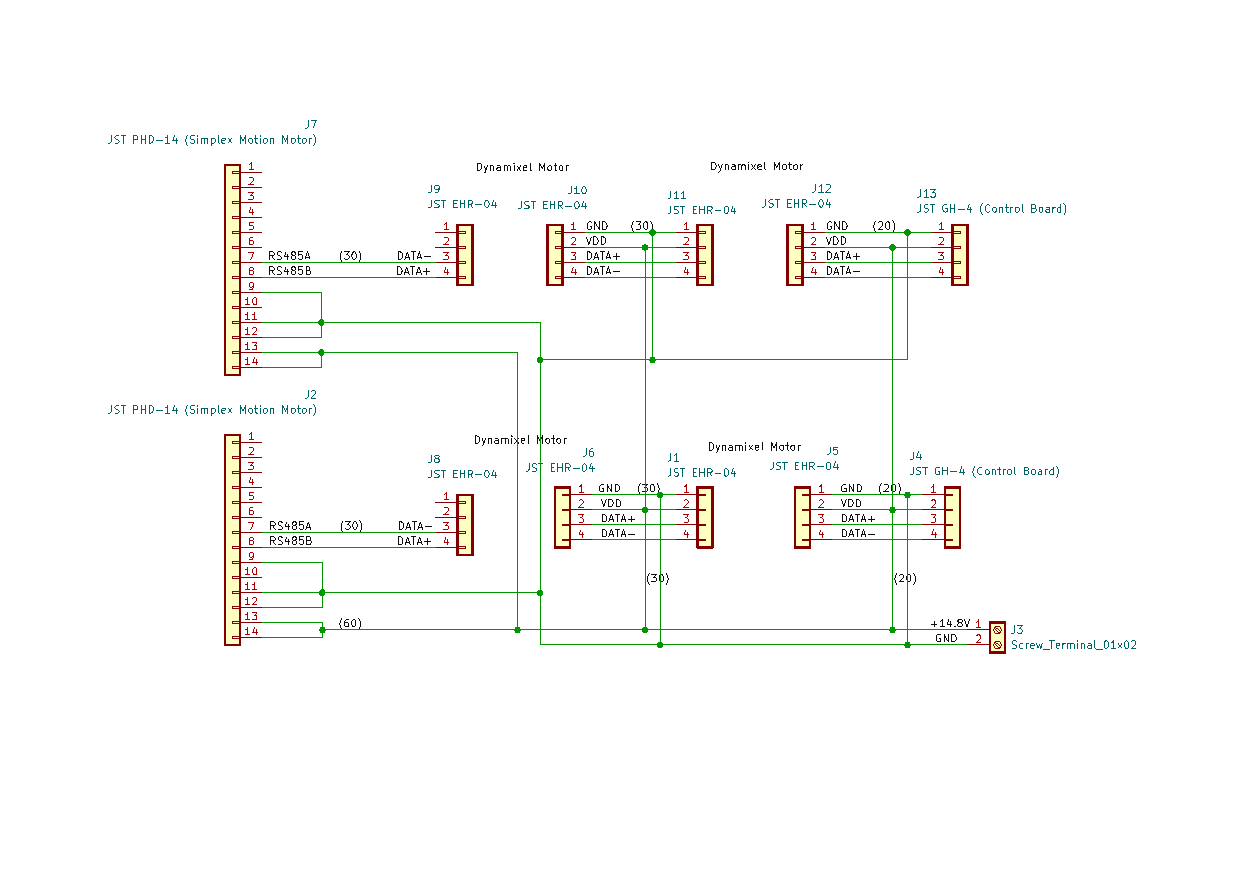
\includegraphics[width=1\linewidth]{Legged_TWIPR_Wiring_Tree}
	%\includegraphics[width=0.5\linewidth]{Figures/Mechanical Design/Conceptual_Design}
	\caption[ brakets for delectronic design second test ]{Electronic Design}
	\label{fig:electronicdesign}
\end{figure}
%expanation of the electronic design
The wiring tree of the electronic components is shown in figure \ref{fig:electronicdesign} where it shows the connection between the different components and the microcontroller.The first motor of each leg is connected to the microcontroller and the rest of the motors are connected in series to the first motor of using daisy chain connection. the motors have the drivers board intigrated so they only need the control signal comimg from the microcontroller.
\begin{itemize}
	\item Provide comprehensive information about the circuit design, including schematic diagrams.
	\item Explain the functionality and interaction of different circuit components.
	\item Discuss the design considerations for signal integrity, power distribution, and noise reduction.
\end{itemize}
\section{PCB (Printed Circuit Board) Design}
\begin{itemize}
	\item Describe the layout and design of any custom PCBs used in the project.
	\item Include information about PCB fabrication and assembly processes.
\end{itemize}
\section{Power Management}
\begin{itemize}
	\item Discuss how power is managed and distributed within the system.
	\item Include details on battery management, voltage regulation, and power efficiency considerations.
\end{itemize}
\chapter{Modelling and Simulation}

\graphicspath{{./Figures/Modeling}}

In this pivotal chapter, we meticulously derive the center of gravity and the moment of inertia for the two-wheeled self-balancing robot. These parameters are the linchpins of our dynamic analysis, serving as the critical variables within the equations of motion that govern the robot's behavior. By calculating these values with precision, we can substitute them into our dynamic equations, thereby tailoring the model to reflect the true dynamics of the robot. This process not only enhances the accuracy of our simulations but also ensures that the control strategies developed are based on a robust and representative model of the robot's physical capabilities. The careful derivation of these parameters is a testament to the thoroughness of our approach, ensuring that the resulting model is both reliable and predictive of the robot's real-world performance.
\newpage

\section{Mathematical Modelling}
\begin{itemize}
	\item \textbf{TWIPR Model:} Explanation of the Two-Wheeled Inverted Pendulum Robot (TWIPR) model.
	
	
	The two wheeled Inverted Pendulum robot model is as shown in the figure where it consist of two legs that include a hip and knee joints as well as wheels at the end of each leg.
	the robot needs to constantly adjust it posture to be able to maintain the balance, just like how the humanbeing balance when standing on the feet.
	
	\item \textbf{Focus on 2D Dynamics:} Discussion on the scope limited to 2D dynamics and plans for future expansion to 3D dynamics and controller synthesis.
	\item \textbf{Assumptions and Parameters:} Detailing assumptions such as considering motor angles as parameters.
	\item \textbf{Model Derivation for \textit{l\_cg} and \textit{I\_y}:} Derivation of the models for center of gravity length (\textit{l\_cg}) and inertia around the y-axis (\textit{I\_y}).
	\item \textbf{Integration into TWIPR Model:} Integration of derived models into a new TWIPR framework.
	\item \textbf{Linear Model Derivation:} Derivation of the linear model from the integrated TWIPR model.
	
	$\bullet$ Modeling allows for predictive analysis and understanding of the robot's behavior.
	
	In order to predict the behavior of the robot under different settings, the modeling procedure entails constructing mathematical representations of the robot's dynamics and control systems.
	
	
	
	\begin{figure}[h]
		\centering
		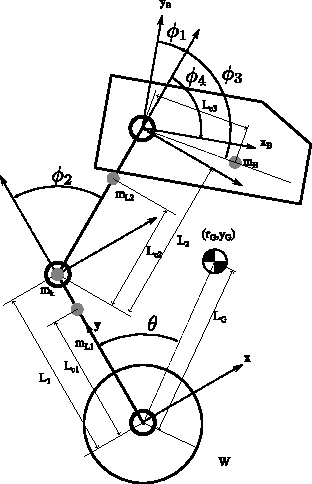
\includegraphics[width=.5\textwidth]{/Model}
		\caption[Mechanical model with the local coordinate system]{Figure illustrating the mechanical model with the local coordinate system to determine the center of gravity.}
		\label{Mechanical model with the local coordinate system}
	\end{figure}
	
	%Center of Gravity
	Center of Gravity calculations 
	\subsection{Center of Gravity } 
	$\bullet$ in that section the calculations of the overall center of gravity 
	
	$\bullet$ Significance in Dynamics:The stability of an object is directly impacted by the COG position, which also affects how it reacts to forces and moments from the outside world.
	
	$\bullet$ maintain equilibrium, 
	
	$\bullet$ accurately determining the COG is crucial for predicting and controlling dynamic behavior
	
	
	in the above figure in order to simplify the deriviation of the center of 
	
	\begin{equation}
		\begin{aligned}
			x_{CG} = \frac{m_{L1} \cdot 0 + m_K \cdot 0 + m_{L2} \cdot L_{C2} \cdot \sin(\phi_2) + m_B \cdot (L_2 \cdot \sin(\phi_2) + L_{C3} \cdot \sin(\phi_2 + \phi_3))}{m_{L1} + m_{L2} + m_K + m_B}
		\end{aligned}
	\end{equation}
	
	\begin{equation}
		\begin{aligned}
			y_{CG} = \frac{m_{L1} \cdot L_{C1} + m_K \cdot L_1 + m_{L2} \cdot (L_1 + L_{C2} \cdot \cos(\phi_2)) + m_B \cdot (L_1 + L_2 \cdot \cos(\phi_2) + L_{C3} \cdot \cos(\phi_2 + \phi_3))}{m_{L1} + m_{L2} + m_K + m_B}
		\end{aligned}
	\end{equation}
	
	%\begin{equation}
	%\begin{aligned}
	%	x_{CG} &= \frac{{m_{L1} L_{C1} \sin(\phi_1) + m_K L_1 \sin(\phi_1) + m_{L2} (L_1 \sin(\phi_1) + L_{C2} \sin(\phi_2 - \phi_1))}}{m_{L1} + m_{L2} + m_K + m_B} \nonumber \\
	%	&\quad + \frac{m_B (L_1 \sin(\phi_1) + L_2 \sin(\phi_2 - \phi_1) + L_{C3} \sin(\phi_3 + \phi_2 - \phi_1))}{m_{L1} + m_{L2} + m_K + m_B}
	%\end{aligned}
	%\end{equation}
	%
	%\begin{equation}
	%\begin{aligned}
	%	y_{CG} &= \frac{{m_{L1} L_{C1} \cos(\phi_1) + m_K L_1 \cos(\phi_1) + m_{L2} (L_1 \cos(\phi_1) + L_{C2} \cos(\phi_2 - \phi_1))}}{m_{L1} + m_{L2} + m_K + m_B} \nonumber \\
	%	&\quad + \frac{m_B (L_1 \cos(\phi_1) + L_2 \cos(\phi_2 - \phi_1) +L_{C3} \cos(\phi_3 + \phi_2 - \phi_1))}{m_{L1} + m_{L2} + m_K + m_B}
	%\end{aligned}
	%\end{equation}
	
	\begin{equation}
		L_G = \sqrt{x_{CG}^2 + y_{CG}^2}
	\end{equation}
	
	\begin{equation}
		\theta = \arctan\left(\frac{{x_{CG}}}{{y_{CG}}}\right)
	\end{equation}
	
	
	\begin{figure}[h]
		\centering
		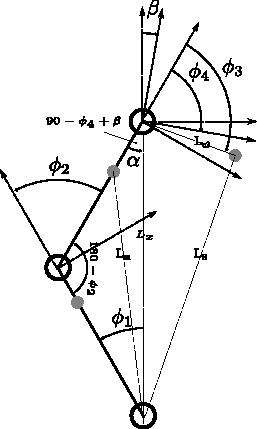
\includegraphics[width=.5\textwidth]{/Angles}
		\caption[Moment of inertia Schematic representation]{Schematic representation detailing the requisite angles and lengths for calculating the moment of inertia.}
		\label{fig:Schematic representation detailing the requisite angles and lengths for calculating the moment of inertia.}
	\end{figure}
	
	\subsection{Moment of inertia}
	%MOI
	Moment of inertia calculations 
	\begin{equation}
		L_m = \sqrt{L_1^2 + L_{C2}^2 - L_1 L_{C2} \cos(180 - \phi_2)}
	\end{equation}
	
	\begin{equation}
		L_{x} = \sqrt{L_1^2 + L_2^2 - L_1 L_2 \cos(180 - \phi_2)}
	\end{equation}
	
	
	\begin{equation}
		\alpha = \cos^{-1} \left( \frac{l_2^2 + l_{x}^2 - l_1^2}{2 l_2 l_{x}} \right) 
	\end{equation}
	
	%\begin{equation}
	%	\alpha = 90 - \phi_4 + \beta
	%\end{equation}
	
	\begin{equation}
		L_b = \sqrt{L_{x}^2 + L_{C3}^2 - Lx L_{C3} \cos(180 - \alpha - \phi_3 )}
	\end{equation}
	
	\begin{equation}
		I_{L1} = \frac{1}{12} m_{L1} (a_1^2 + b_1^2)
	\end{equation}
	\begin{equation}
		I_{L2} = \frac{1}{12} m_{L1} (a_2^2 + b_2^2)
	\end{equation}
	\begin{equation}
		I_K = \frac{1}{2} m_K R_m^2
	\end{equation}
	\begin{equation}
		I_B = \frac{1}{12} m_B (a_B^2 + b_B^2)
	\end{equation}
	\begin{equation}
		I = I_{L1} + m_{L1} L_{C1}^2 + I_K + m_K L_1^2 + I_{L2} + m_{L2} L_m^2 + I_B + m_B L_b^2
	\end{equation}
	
	\subsection{Equation of motion }
	%equation of motion 
	Equation of motion 
	
	
	
	
	
	
	\subsection{Dynamics of the Two-Wheeled Inverted Pendulum Robot}
	Given the functions $B_i: \mathbb{R} \rightarrow \mathbb{R}$, $C_{ij}: \mathbb{R} \rightarrow \mathbb{R}$, $D_{ij}: \mathbb{R} \rightarrow \mathbb{R}$, and $V_i: \mathbb{R} \rightarrow \mathbb{R}$, $i,j \in \{1,2,3\}$, the equations of motion are given by:
	
	\begin{align}
		\ddot{s} &= \frac{\sin(\Theta)}{V_1(\Theta)} \left( -C_{11}(\Theta) + C_{12}\dot{\Theta}^2 + C_{13}(\Theta)\dot{\psi}^2 \right) - \frac{D_{11}(\Theta)}{V_1(\Theta)}\dot{s} + \frac{D_{12}(\Theta)}{V_1(\Theta)}\dot{\Theta} + \frac{B_{1}(\Theta)}{V_1(\Theta)}(\tau_L + \tau_R) \\
		\ddot{\Theta} &= \frac{\sin(\Theta)}{V_1(\Theta)} \left( C_{21} - C_{22}(\Theta)\dot{\Theta}^2 - C_{23}(\Theta)\dot{\psi}^2 \right) + \frac{D_{21}(\Theta)}{V_1(\Theta)}\dot{s} - \frac{D_{22}(\Theta)}{V_1(\Theta)}\dot{\Theta} - \frac{B_{2}(\Theta)}{V_1(\Theta)}(\tau_L + \tau_R)  \\
		\ddot{\psi} &= \frac{\sin(\Theta)}{V_2(\Theta)} \left( C_{31}(\Theta)\dot{\Theta}\dot{\psi} - C_{32}(\Theta)\dot{\psi}\dot{s} \right) - \frac{D_{33}(\Theta)}{V_2(\Theta)}\dot{\psi} - \frac{B_{3}}{V_2(\Theta)}(\tau_L - \tau_R)
	\end{align}
	
	
	The equations of motion are derived in [44]. The functions $B_i: \mathbb{R} \rightarrow \mathbb{R}$, $C_{ij}: \mathbb{R} \rightarrow \mathbb{R}$, $D_{ij}: \mathbb{R} \rightarrow \mathbb{R}$, and $V_i: \mathbb{R} \rightarrow \mathbb{R}$, $i,j \in \{1,2,3\}$, are given by:
	
	\begin{equation}
		C_{11}(\Theta) = m_B^2 l^2 \cos(\Theta),
	\end{equation}
	\begin{equation}
		C_{12} = (I_2 + m_B l^2) m_B l,
	\end{equation}
	\begin{equation}
		C_{13}(\Theta) = (I_2 + m_B l^2) m_B l + m_B l (I_3 - I_1 - m_B l^2) \cos^2(\Theta),
	\end{equation}
	\begin{equation}
		C_{21} = (m_B + 2m_W + \frac{2J}{r^2}) m_B l,
	\end{equation}
	\begin{equation}
		C_{22}(\Theta) = m_B^2 l^2 \cos(\Theta),
	\end{equation}
	\begin{equation}
		C_{23}(\Theta) = m_B^2 l^2 + (m_B + 2m_W + \frac{2J}{r^2}) (I_3 - I_1 - m_B l^2) \cos(\Theta).
	\end{equation}
	\begin{equation}
		C_{31}(\Theta) = 2 (I_3 - I_1 - m_B^2) \cos(\Theta),
	\end{equation}
	\begin{equation}
		C_{31} = m_B l,
	\end{equation}
	\begin{equation}
		D_{11}(\Theta) = \frac{(I_2 + m_B^2) 2c_\alpha}{r^2} - \frac{m_B \cos(\Theta) 2c_\alpha}{r},
	\end{equation}
	\begin{equation}
		D_{12}(\Theta) = \frac{(I_2 + m_B^2) 2c_\alpha}{r} - 2m_B \cos(\Theta) c_\alpha,
	\end{equation}
	\begin{equation}
		D_{21}(\Theta) = \frac{(m_B + 2m_W + \frac{2J}{r^2}) 2c_\alpha}{r} + \frac{m_B \cos(\Theta) 2c_\alpha}{r^2},
	\end{equation}
	\begin{equation}
		D_{22}(\Theta) = \frac{(m_B + 2m_W + \frac{2J}{r}) 2c_\alpha + m_B \cos(\Theta) 2c_\alpha}{r},
	\end{equation}
	\begin{equation}
		D_{33}(\Theta) = \frac{d^2}{2r^2 c_\alpha},
	\end{equation}
	\begin{equation}
		B_{1} = \frac{(I_2 + m_B^2) \frac{1}{r} + m_B \cos(\Theta)}{r},
	\end{equation}
	\begin{equation}
		B_{2} = \frac{m_B l}{r} - \cos(\Theta) + m_B + 2m_W + \frac{2J}{r^2},
	\end{equation}
	\begin{equation}
		B_{3} = \frac{d}{2r},
	\end{equation}
	\begin{equation}
		V_{1} = (m_B + 2m_W + \frac{2J}{r^2}) (I_2 + m_B^2) - m_B^2 \cos^2(\Theta),
	\end{equation}
	\begin{equation}
		V_{2} = I_3 + 2K + (m_W + \frac{J}{r^2}) \frac{d^2}{2} - (I_3 - I_1 - m_B^2) \sin^2(\Theta).
	\end{equation}
	
	
	\begin{table}[h!]
		\centering
		\caption{Parameters of the mechanical system}
		\label{tab:parameters}
		\begin{tabular}{lcl}
			\toprule
			Parameter & Value & Description \\
			\midrule
			$m_B$ & 2.5 kg & mass of the pendulum body \\
			$m_W$ & 0.636 kg & mass of a wheel \\
			$l$ & 0.026 m & distance between the wheel axis and the pendulum's center of gravity \\
			$d$ & - & distance between the two wheels \\
			$J$ & \(5.175 e^{-4}\) kgm\textsuperscript{2} & moment of inertia of a wheel w.r.t. reference frame \{C\} in direction of \(c_2\) \\
			$K$ & - & moment of inertia of a wheel w.r.t. reference frame \{C\} in direction of \(c_3\) \\
			$I_1$ & - & moment of inertia of pendulum's body w.r.t. reference frame \{B\} in direction of \(b_1\) \\
			$I_2$ & \(0.0165\) kgm\textsuperscript{2} & moment of inertia of pendulum's body w.r.t. reference frame \{B\} in direction of \(b_2\) \\
			$I_3$ & - & moment of inertia of pendulum's body w.r.t. reference frame \{B\} in direction of \(b_3\) \\
			$c_\alpha$ & \(4.630 e^{-4}\) Nms & viscous friction coefficient \\
			\bottomrule
		\end{tabular}
	\end{table}
\end{itemize}

\section{Numerical Simulation}
\begin{itemize}
	\item \textbf{Discrete Numerical Simulation:} Elaboration on the process of discrete numerical simulation, including the discrete double integration method to arrive at the state vector.
\end{itemize}

\section{Simulation Environment}
\begin{itemize}
	\item \textbf{Overview of the Simulation Environment:} A brief overview of the simulation environment, referencing David's Bachelor Thesis for details.
	
	
	\item \textbf{Integration of the Model:} Description of integrating the new TWIPR model into the simulation environment and a summary of the individual components of the model.
\end{itemize}

\section{Controller Synthesis}
\begin{itemize}
	\item \textbf{State-Space Controllers:} Introduction to two state-space controllers: Linear Quadratic Regulator (LQR) and Pole-Placement.
	\item \textbf{Configuration Specificity:} Explanation of how these controllers are specific to one configuration (knee angle and hip angle) of the robot.
	\item \textbf{Controller Retuning Algorithm:} Presentation of an algorithm for retuning the controllers as the configuration changes.
\end{itemize}

\section{Simulation Analysis}
\begin{itemize}
	\item \textbf{Controller Responses:} Analysis of step response and responses to other inputs using one of the controllers in different configurations.
	\item \textbf{Impact of Non-Retuning:} Discussion on the effects of not retuning the controllers.
	\item \textbf{Influence of Leg Configuration:} Analysis of how leg configuration influences the robot's behavior.
	\item \textbf{Controller Setting Comparisons:} Comparative study of different controller settings and a comparison between LQR and Pole-Placement controllers.
	\item \textbf{Optimal Controller Configuration:} Conclusion on which controller configuration might be best suited for such a robot.
\end{itemize}










	



\chapter{Mechanical Assembly}

\graphicspath{{./Figures/Mechanical Assembly/}}

%\begin{itemize}
%	\item Intro Overview of the chapter.
%	\item Importance of mechanical assembly in the overall project.
In this chapter, the mechanical assembly of the robot is discussed.
The mechanical assembly is the process of putting together the mechanical components of the robot.
The mechanical components include the chassis which is composed of several parts, the wheels, the motors.
The assembly process is described in detail, including the tools and techniques used.
The integration of the mechanical and electronic systems is also discussed.
The challenges faced during the assembly process are described, along with the troubleshooting and problem-solving strategies employed.
Finally, the safety considerations taken during the assembly process are discussed.
, the wheels, the motors.
%\end{itemize}
\newpage

\section{Components Overview}

%\begin{itemize}
%\item Detailed description of all mechanical components used in the robot.
%\item Source or method of fabrication for each component (e.g., machined parts, 3D printed elements).
%\end{itemize}
As shown in the mechanical design chapter, the robot is composed of several mechanical components.The body, hip knee links, knee wheel links, board mounting rack, Wheel motor cover, body cover and body face shield.
These components were printed using a 3D printer with different configuration for each part.Other components such as the wheels, motors, motor shaft hub, screws and thread inserts were bought from the market.
\section{Fabrication}
% figure for printing the body
\begin{figure}[h]
	\centering
	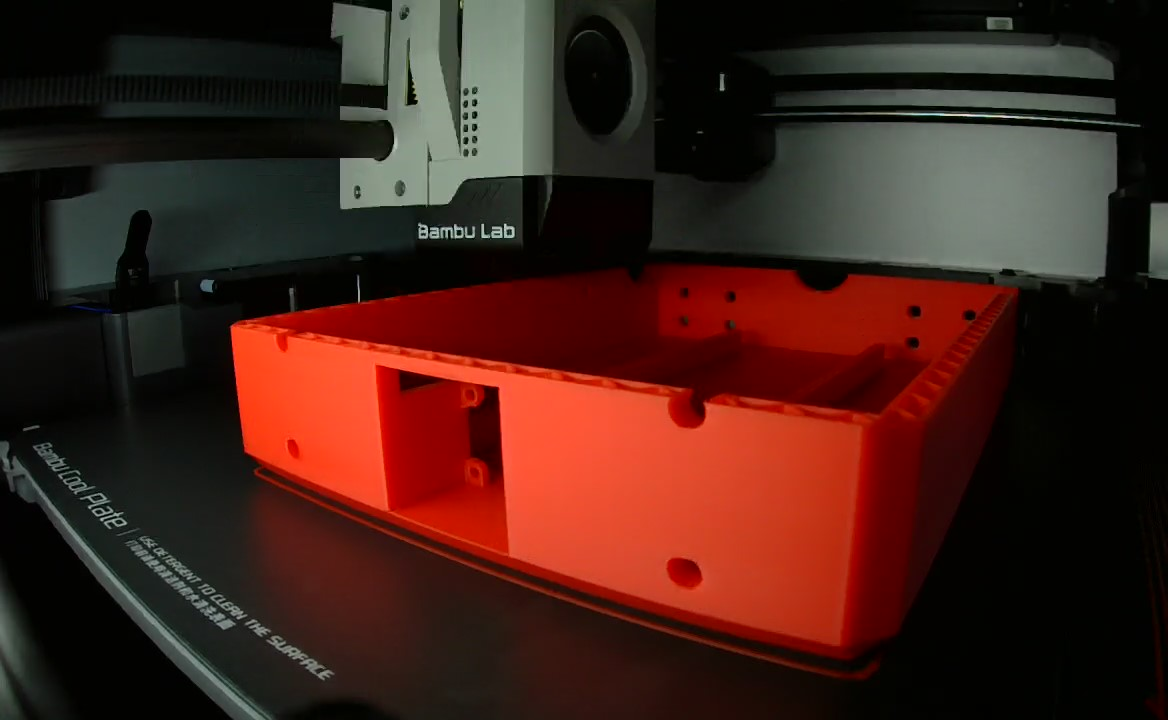
\includegraphics[width=0.7\linewidth]{body_printing}
	\caption{Printing the body}
	\label{fig:bodyprinting}
\end{figure}
The print infill, orientation material and layer height were changed to suit the part.
Fifty percent infill was used for the body, and seventy percent infill was used for links to make them strong enough to withstand the forces applied on them and to avoid breaking at weak points.
The orientation of the parts was changed to make the print stronger and to avoid the need for support material.
The aim was to make the printed layers perpendicular to the forces applied on the part.
PLA was used as the printing material for all the parts except for the body face shield which was printed using TPU to make it flexible.
%figure of the design techniques used
\begin{figure}[h]
	\centering
	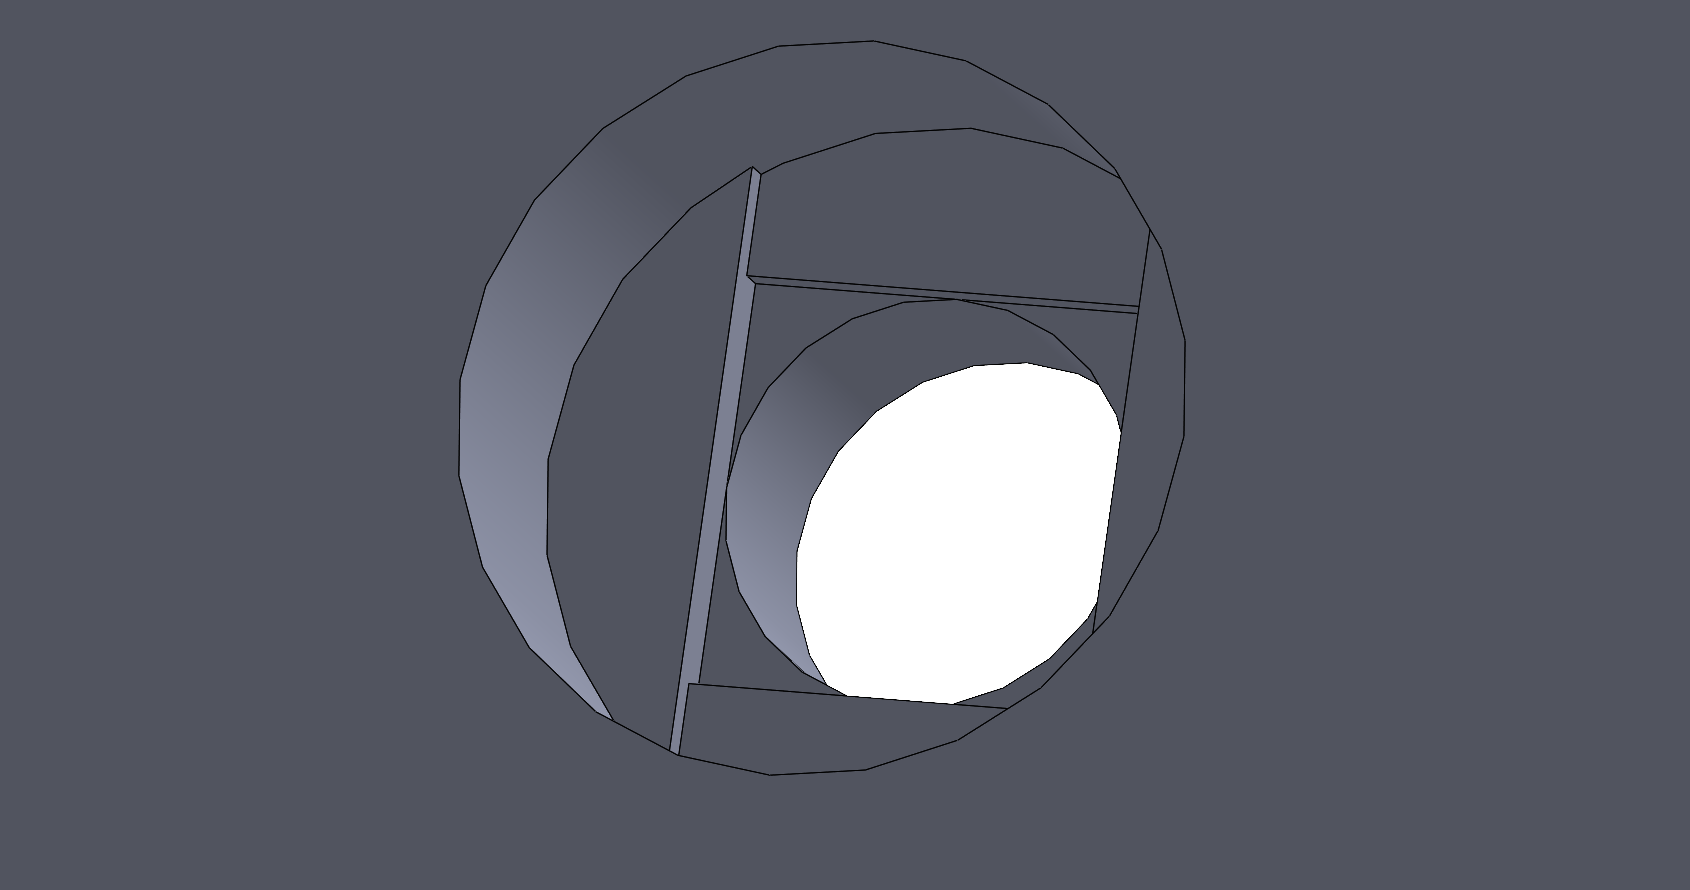
\includegraphics[width=0.5\linewidth]{screw_head_fitting}
	\caption{Design techniques used to avoid the need for support material}
	\label{fig:Screw head fitting}
\end{figure}
Different design techniques as shown in figure \ref{fig:Screw head fitting}were used specially for the place where the socket screws heads are inserted to avoid the need for support material.
\section{Assembly Process}
\subsection{Motors Assembly}
%the process of assembling the motors to be ready to be mounted on the chassis.
The hip and knee motors required assembly before they could be mounted on the chassis.
%%Two subfigures side by side of the hip_knee_motors_assembly and the horn_assembly_marking
\begin{figure}[h]
	\centering
	\begin{subfigure}[t]{0.45\textwidth}
		\centering
		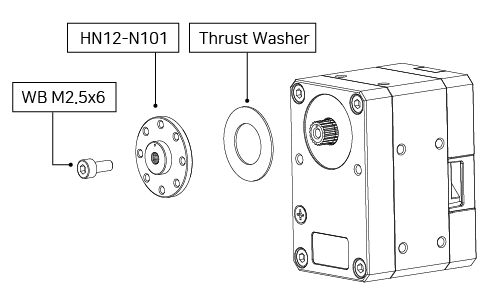
\includegraphics[height=0.7\textwidth]{hip_knee_motors_assembly}
		\caption{Hip and knee motors assembly}
		\label{fig:hipkneemotorsassembly}
	\end{subfigure}
	\begin{subfigure}[t]{0.45\textwidth}
		\centering
		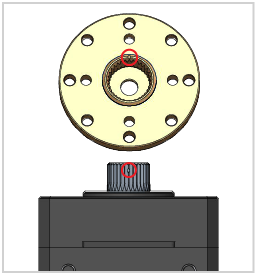
\includegraphics[height=0.7\textwidth]{horn_assembly_marking}
		\caption{Horn assembly marking}
		\label{fig:horn_assembly_marking}
	\end{subfigure}
	\caption{Comparison between the hip and knee motors assembly and the horn assembly marking}
	\label{fig:Comparison between the hip and knee motors assembly and the horn assembly marking}
\end{figure}

The assembly process is shown in figure \ref{fig:hipkneemotorsassembly} shows the normal horn assembly. the thrust washer should be placed between the horn and the motor to avoid friction between the horn and the motor. the horn should be tightened using the screw.As shown in figure \ref{fig:horn_assembly_marking} the indexing mark on the output horn is aligned with the index marking on the output shaft.

%figure for the motor spacer ring
\begin{figure}[h]
	\centering
	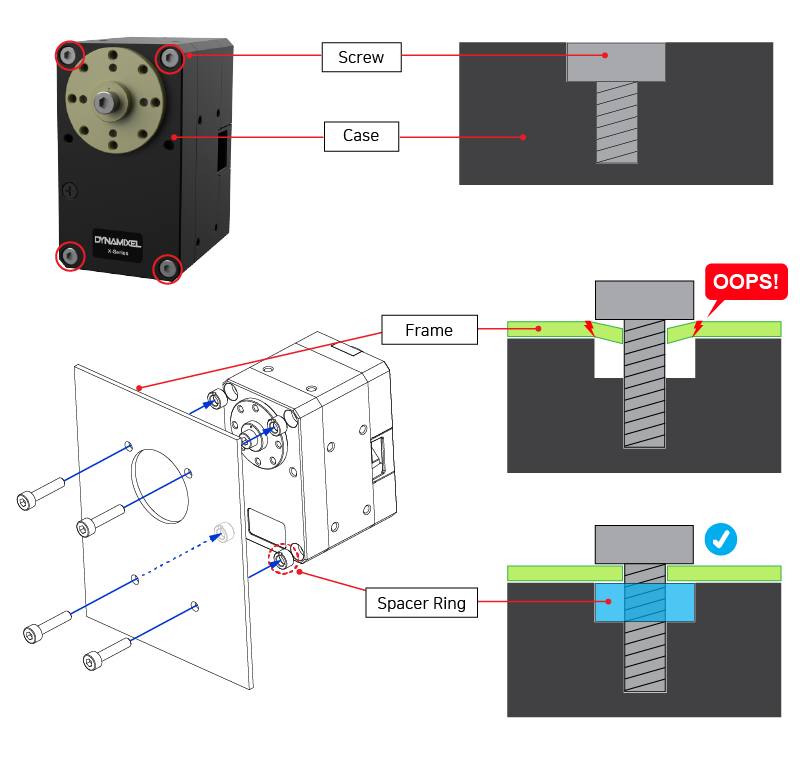
\includegraphics[width=0.5\linewidth]{motor_spacer_ring}
	\caption{Motor spacer ring}
	\label{fig:motorspacerring}
\end{figure}
The motor spacer ring shown in figure \ref{fig:motorspacerring} was used to make to fill the gap between the motor case and chassis frame.
The frame thickness was added to the length of the new screw to make sure that the screw is not larger than the depth of the mounting point or the motor case may be damaged.

\subsection{Screws and thread inserts}
The screws and thread inserts used in the assembly are shown in the table\ref{tab:screws}.The precise dimensions of the screws and thread inserts were important to make sure that the assembly process goes smoothly.
The tolerance of 0.1 mm for the screws was acceptable for the assembly process except for the screws used for the hip and knee motors horns as it could touch the thrust washer and cause damage to the motor.

%table for the screws and thread inserts used in the assembly
\begin{table}[h!]
	\centering
	\caption{Screws and thread inserts used in the assembly}
	\label{tab:screws}
	\begin{tabular}{lcl}
		\toprule
		Component & Quantity & Screw size \\
		\midrule
		Wheel Motor & 8 & M3*8 \\
		Knee Motor Horn & 16 & M2*13 \\
		Knee Motor front & 8 & M2.5*14 \\
		Knee Motor Top & 8 & M2.5*5 \\
		Knee Motor sides & 20 & M2.5*5 or M2.5*5 .5 \\
		Hip Motor front & 8 & M2.5*6 \\
		Hip Motor Horn & 16 & M2*15 \\
		Hip Motor side & 8 & M2.5*15 \\
		Body & 12 & M2.5*6 \\
		Wheel Motor cover & 20 & M2.5*6 \\
		thread inserts & 36 & M2.5 x 5.7 \\
		\bottomrule
	\end{tabular}
\end{table}


%\ref{tab:screws}.
\subsection{Chassis Assembly}
%figure for the assembled chassis
\begin{figure}[h]
	\centering
	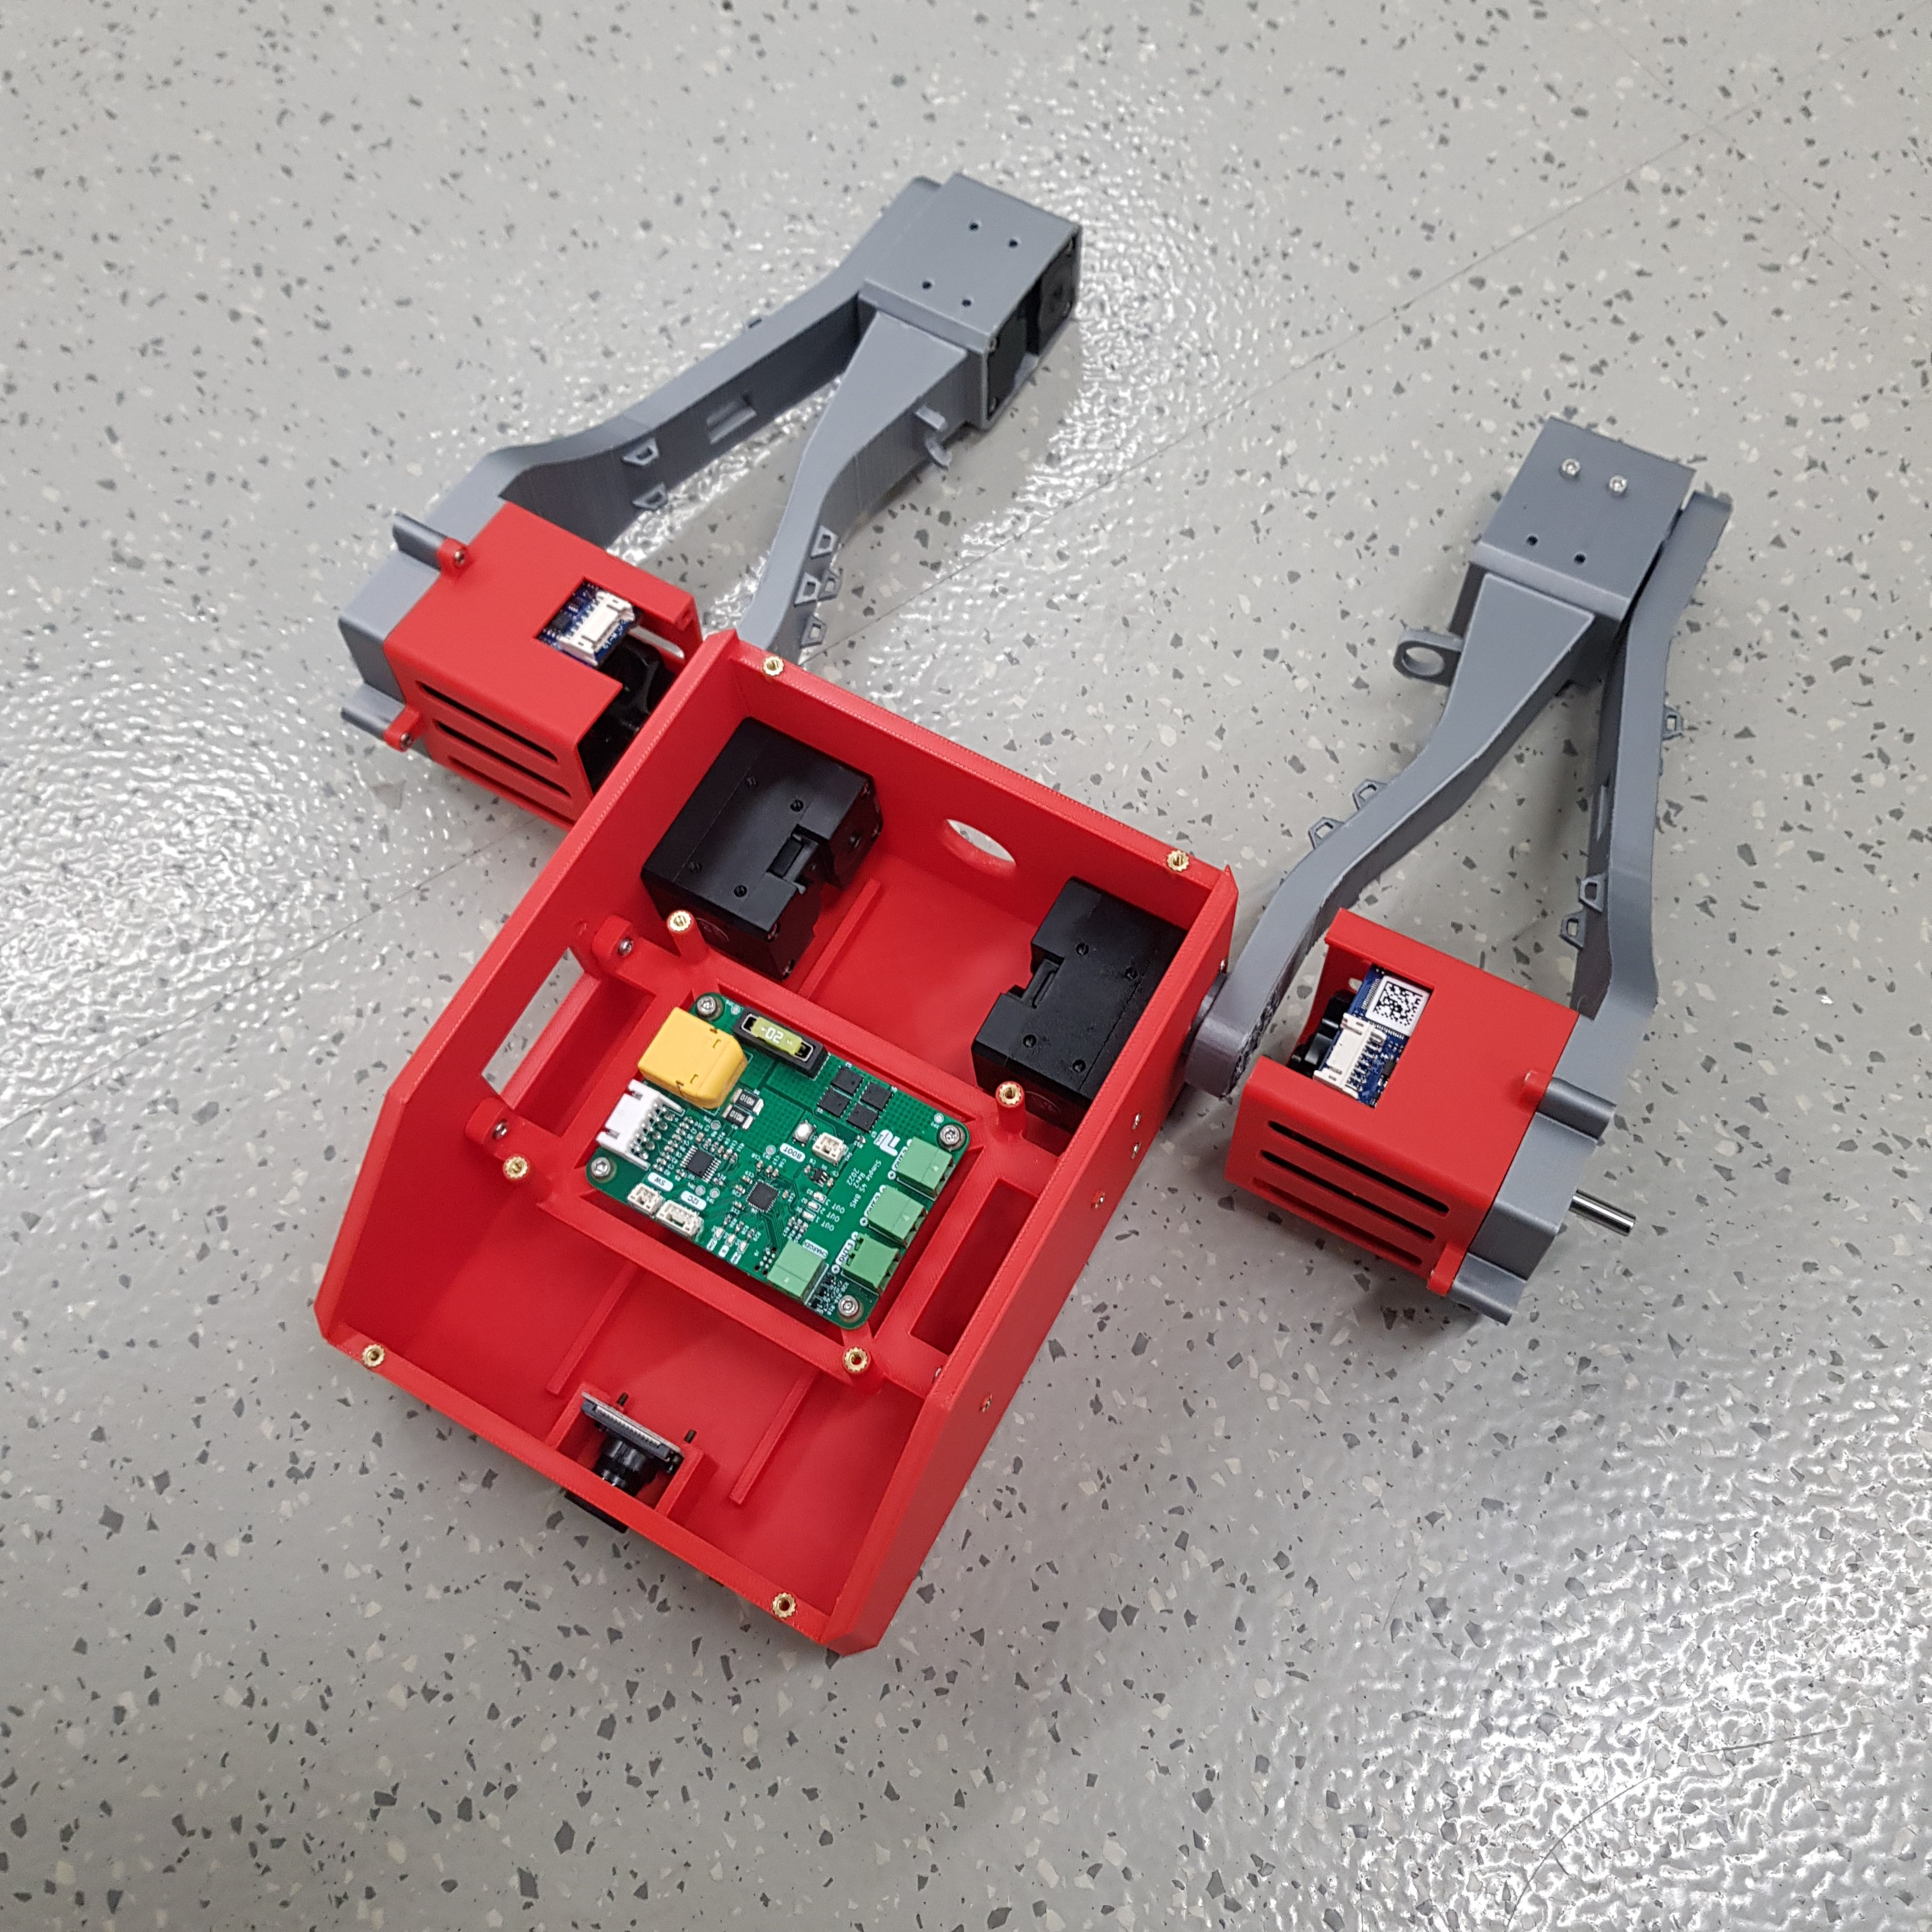
\includegraphics[width=0.5\linewidth]{chassis_assembled}
	\caption{Assembled chassis}
	\label{fig:chassisassembled}
\end{figure}
%\begin{itemize}
%\item Step-by-step explanation of the assembly process.
The assembly process started with the chassis, the chassis was assembled using screws and thread inserts.
First the thread inserts were inserted into the chassis using soldering iron, then the screws were used to assemble the motors to the knee wheel links, the hip knee links, the body.
then the knee wheel links were assembled to the hip knee links

%\item Tools and techniques used in the assembly.
%\item Assembly sequence and rationale behind it.
%\end{itemize}
\newpage
%several figures for the assembly process of the chassis
%three subfigures for the thread inserts (Body thread inserts, knee wheel link thread inserts, Board mounting rack thread inserts)
\begin{figure}[h]
	\centering
	\begin{subfigure}[t]{0.3\textwidth}
		\centering
		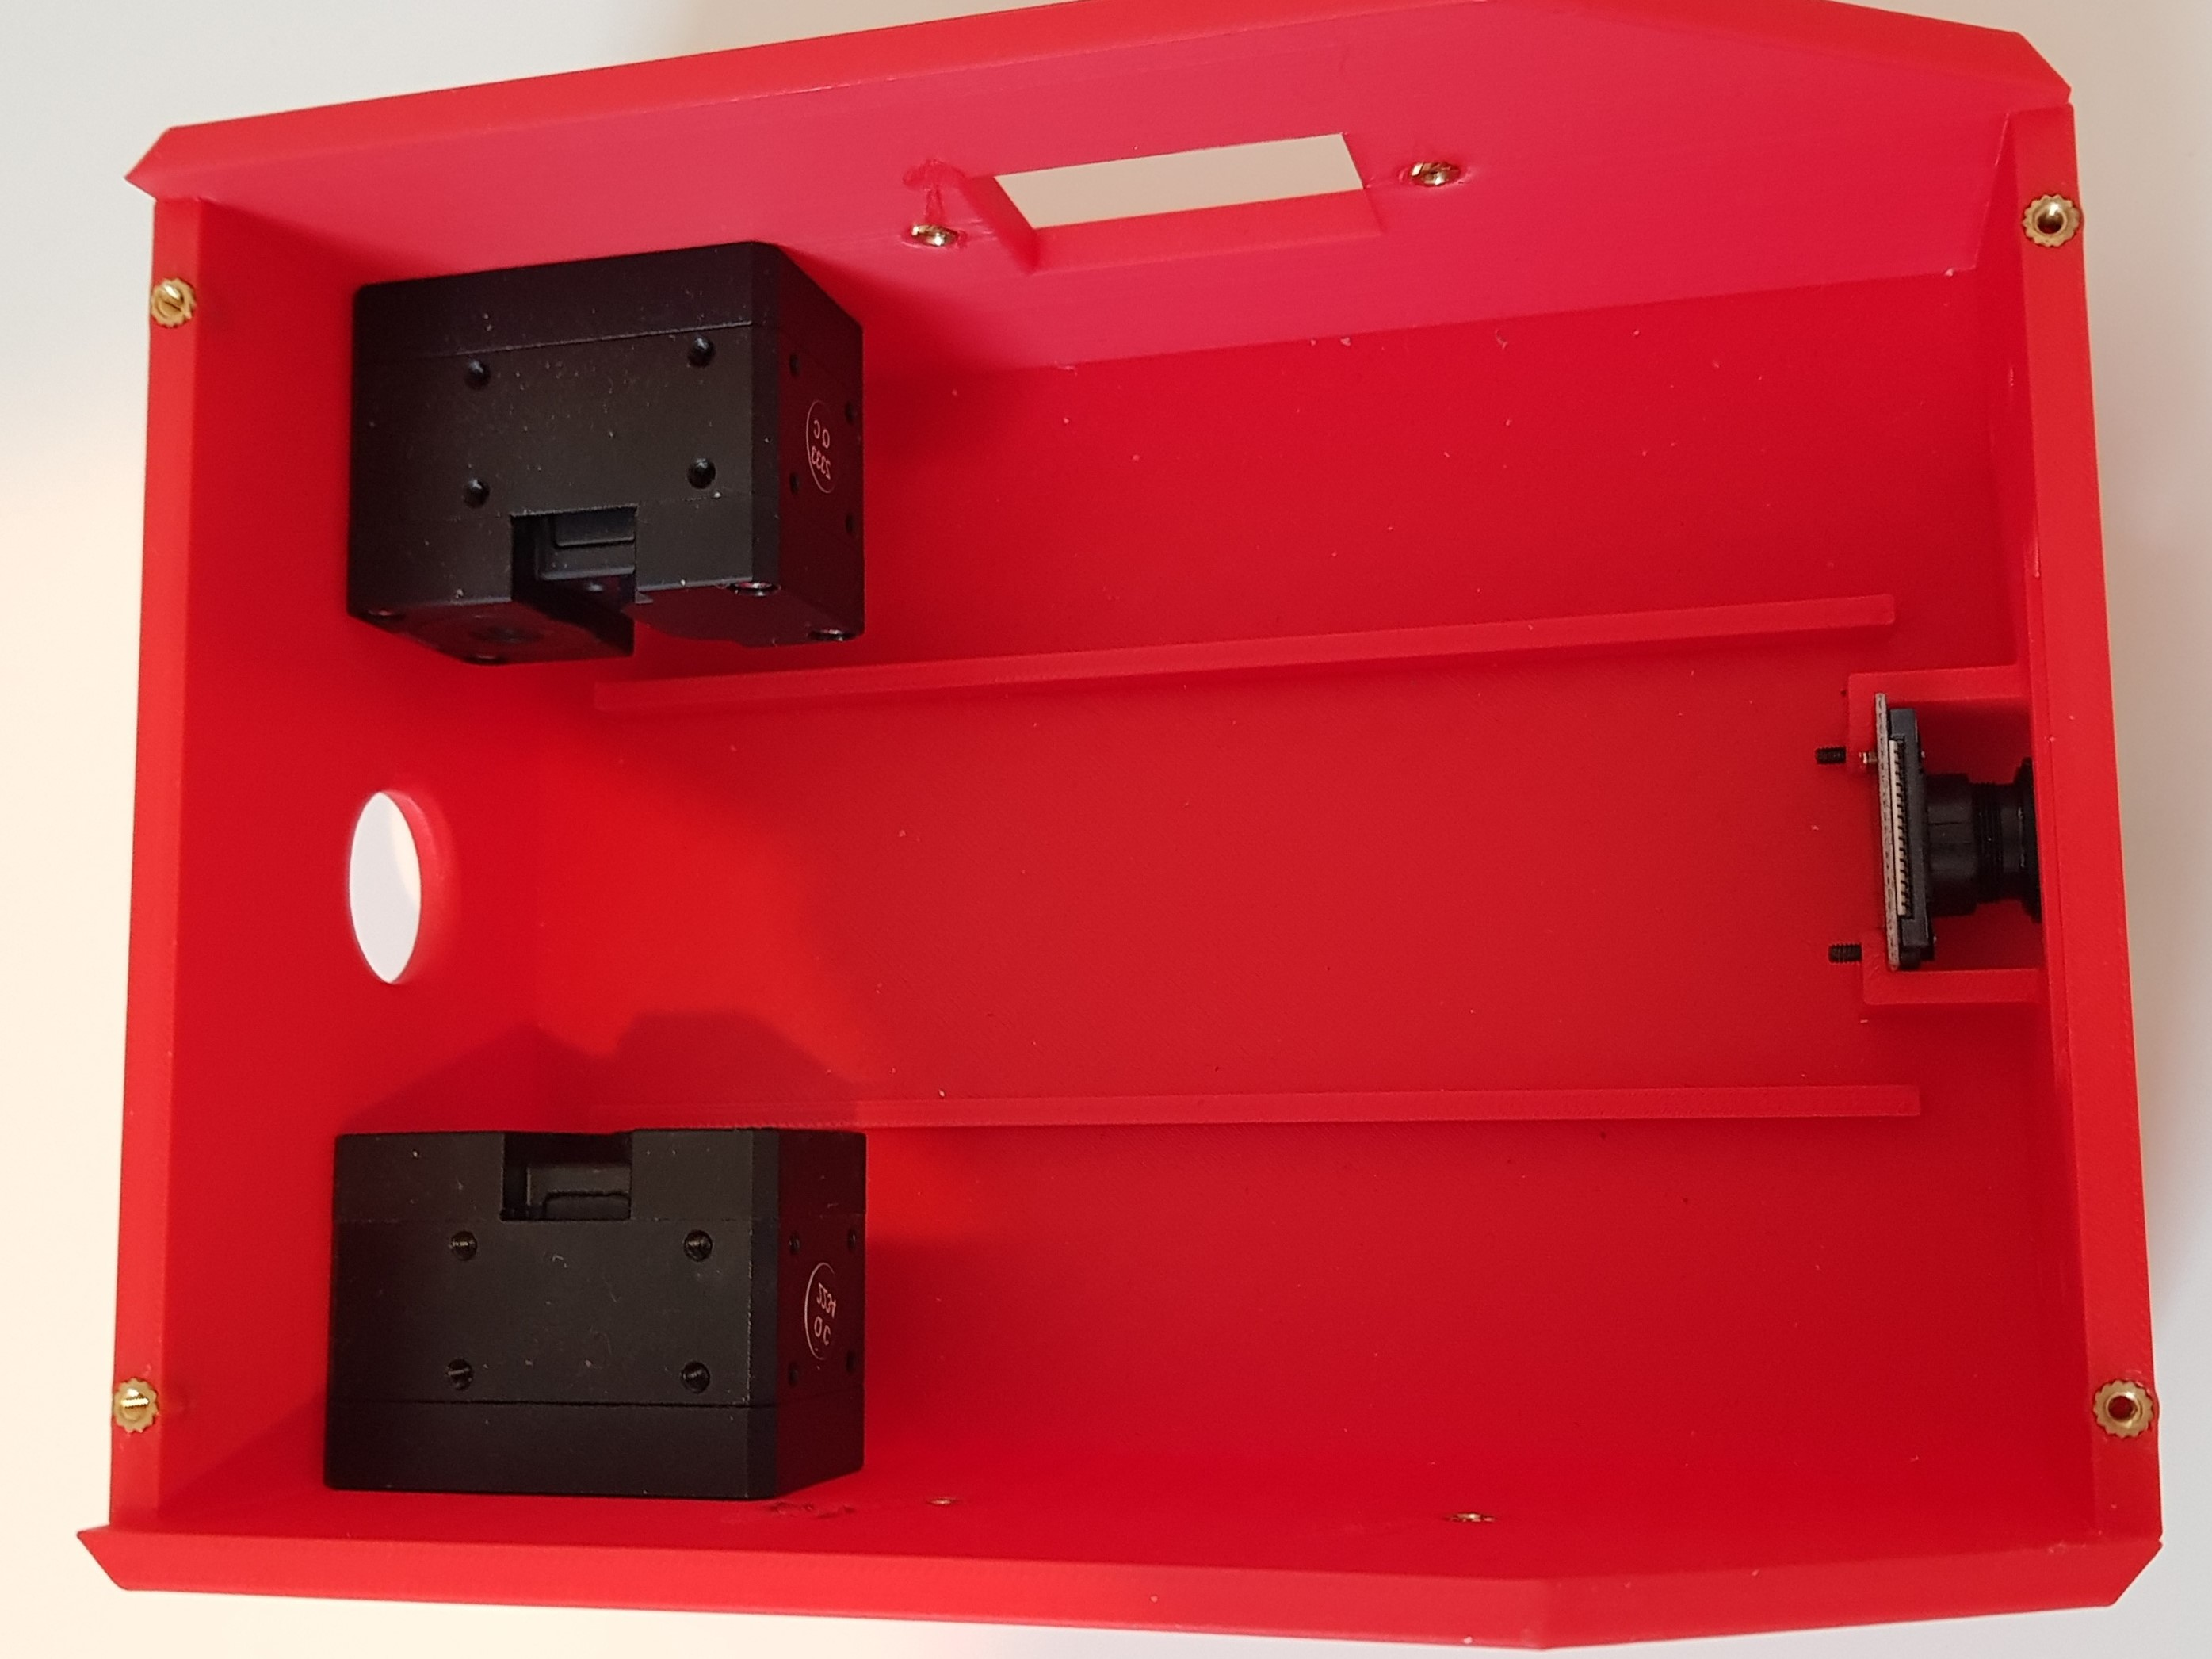
\includegraphics[height=0.7\textwidth]{body_thread_inserts}
		\caption{Body thread inserts}
		\label{fig:bodythreadinserts}
	\end{subfigure}
	\begin{subfigure}[t]{0.3\textwidth}
		\centering
		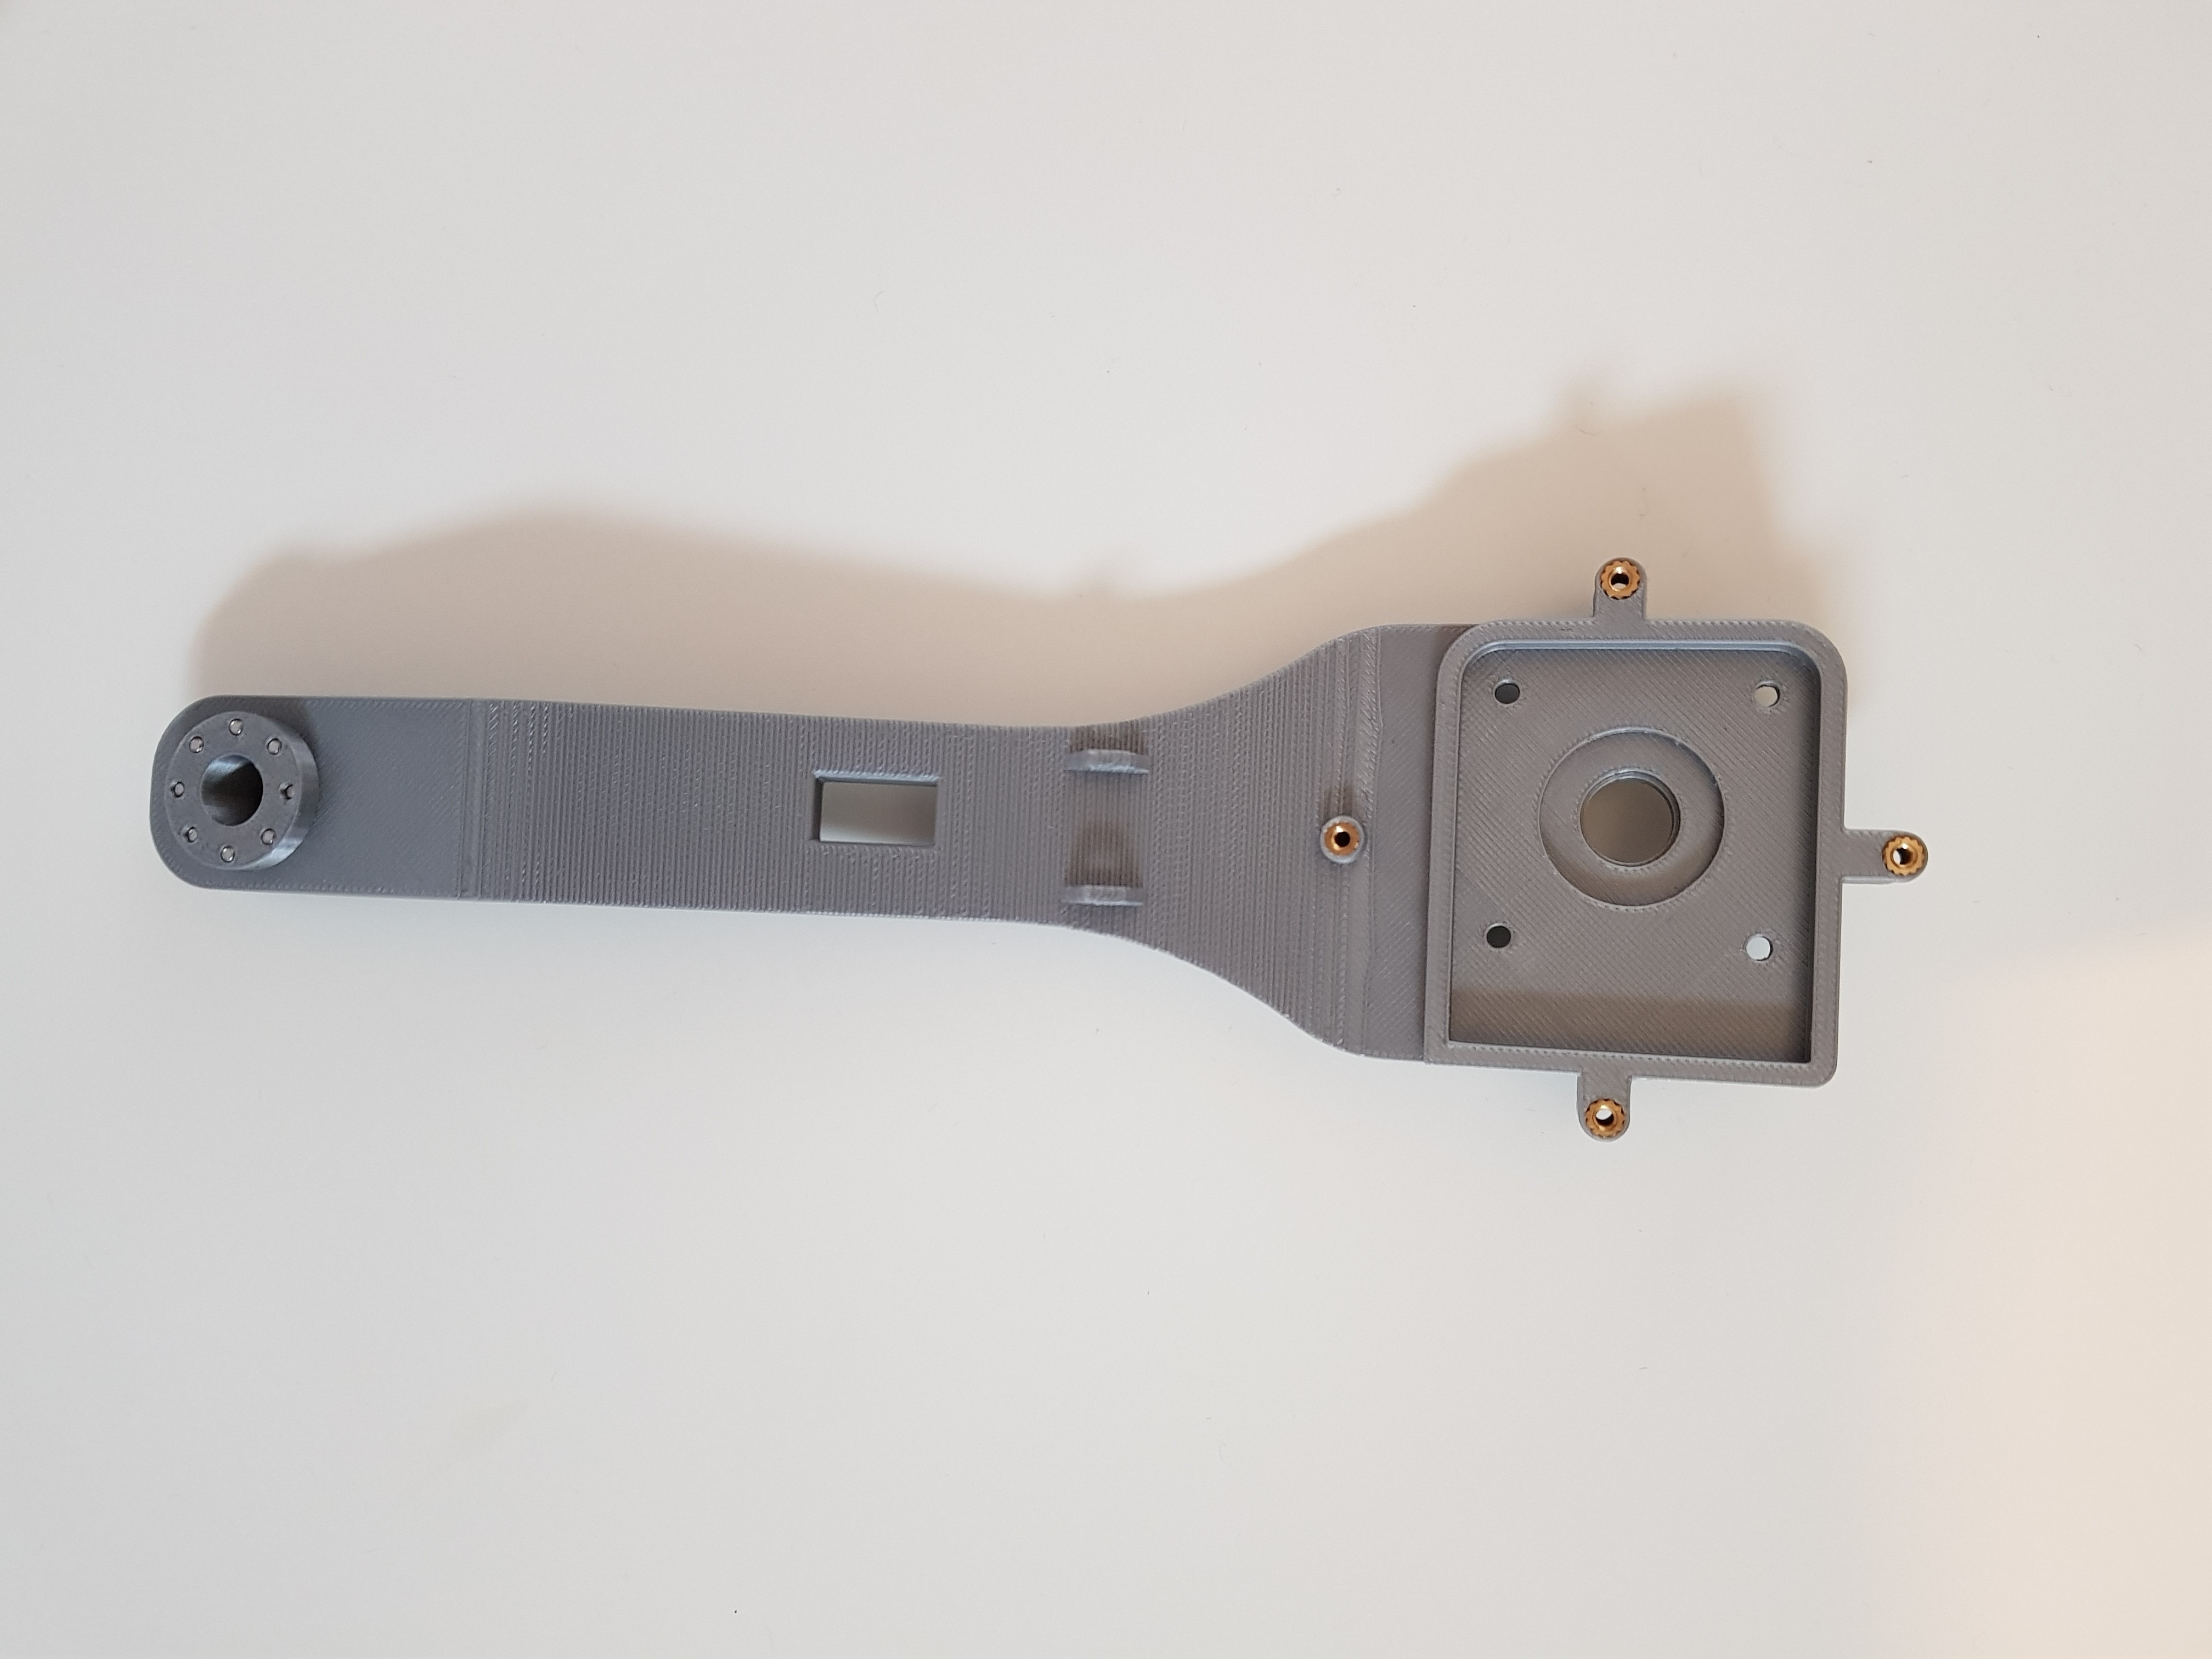
\includegraphics[height=0.7\textwidth]{knee_wheel_link_thread_inserts}
		\caption{Knee wheel link thread inserts}
		\label{fig:kneewheellinkthreadinserts}
	\end{subfigure}
	\begin{subfigure}[t]{0.3\textwidth}
		\centering
		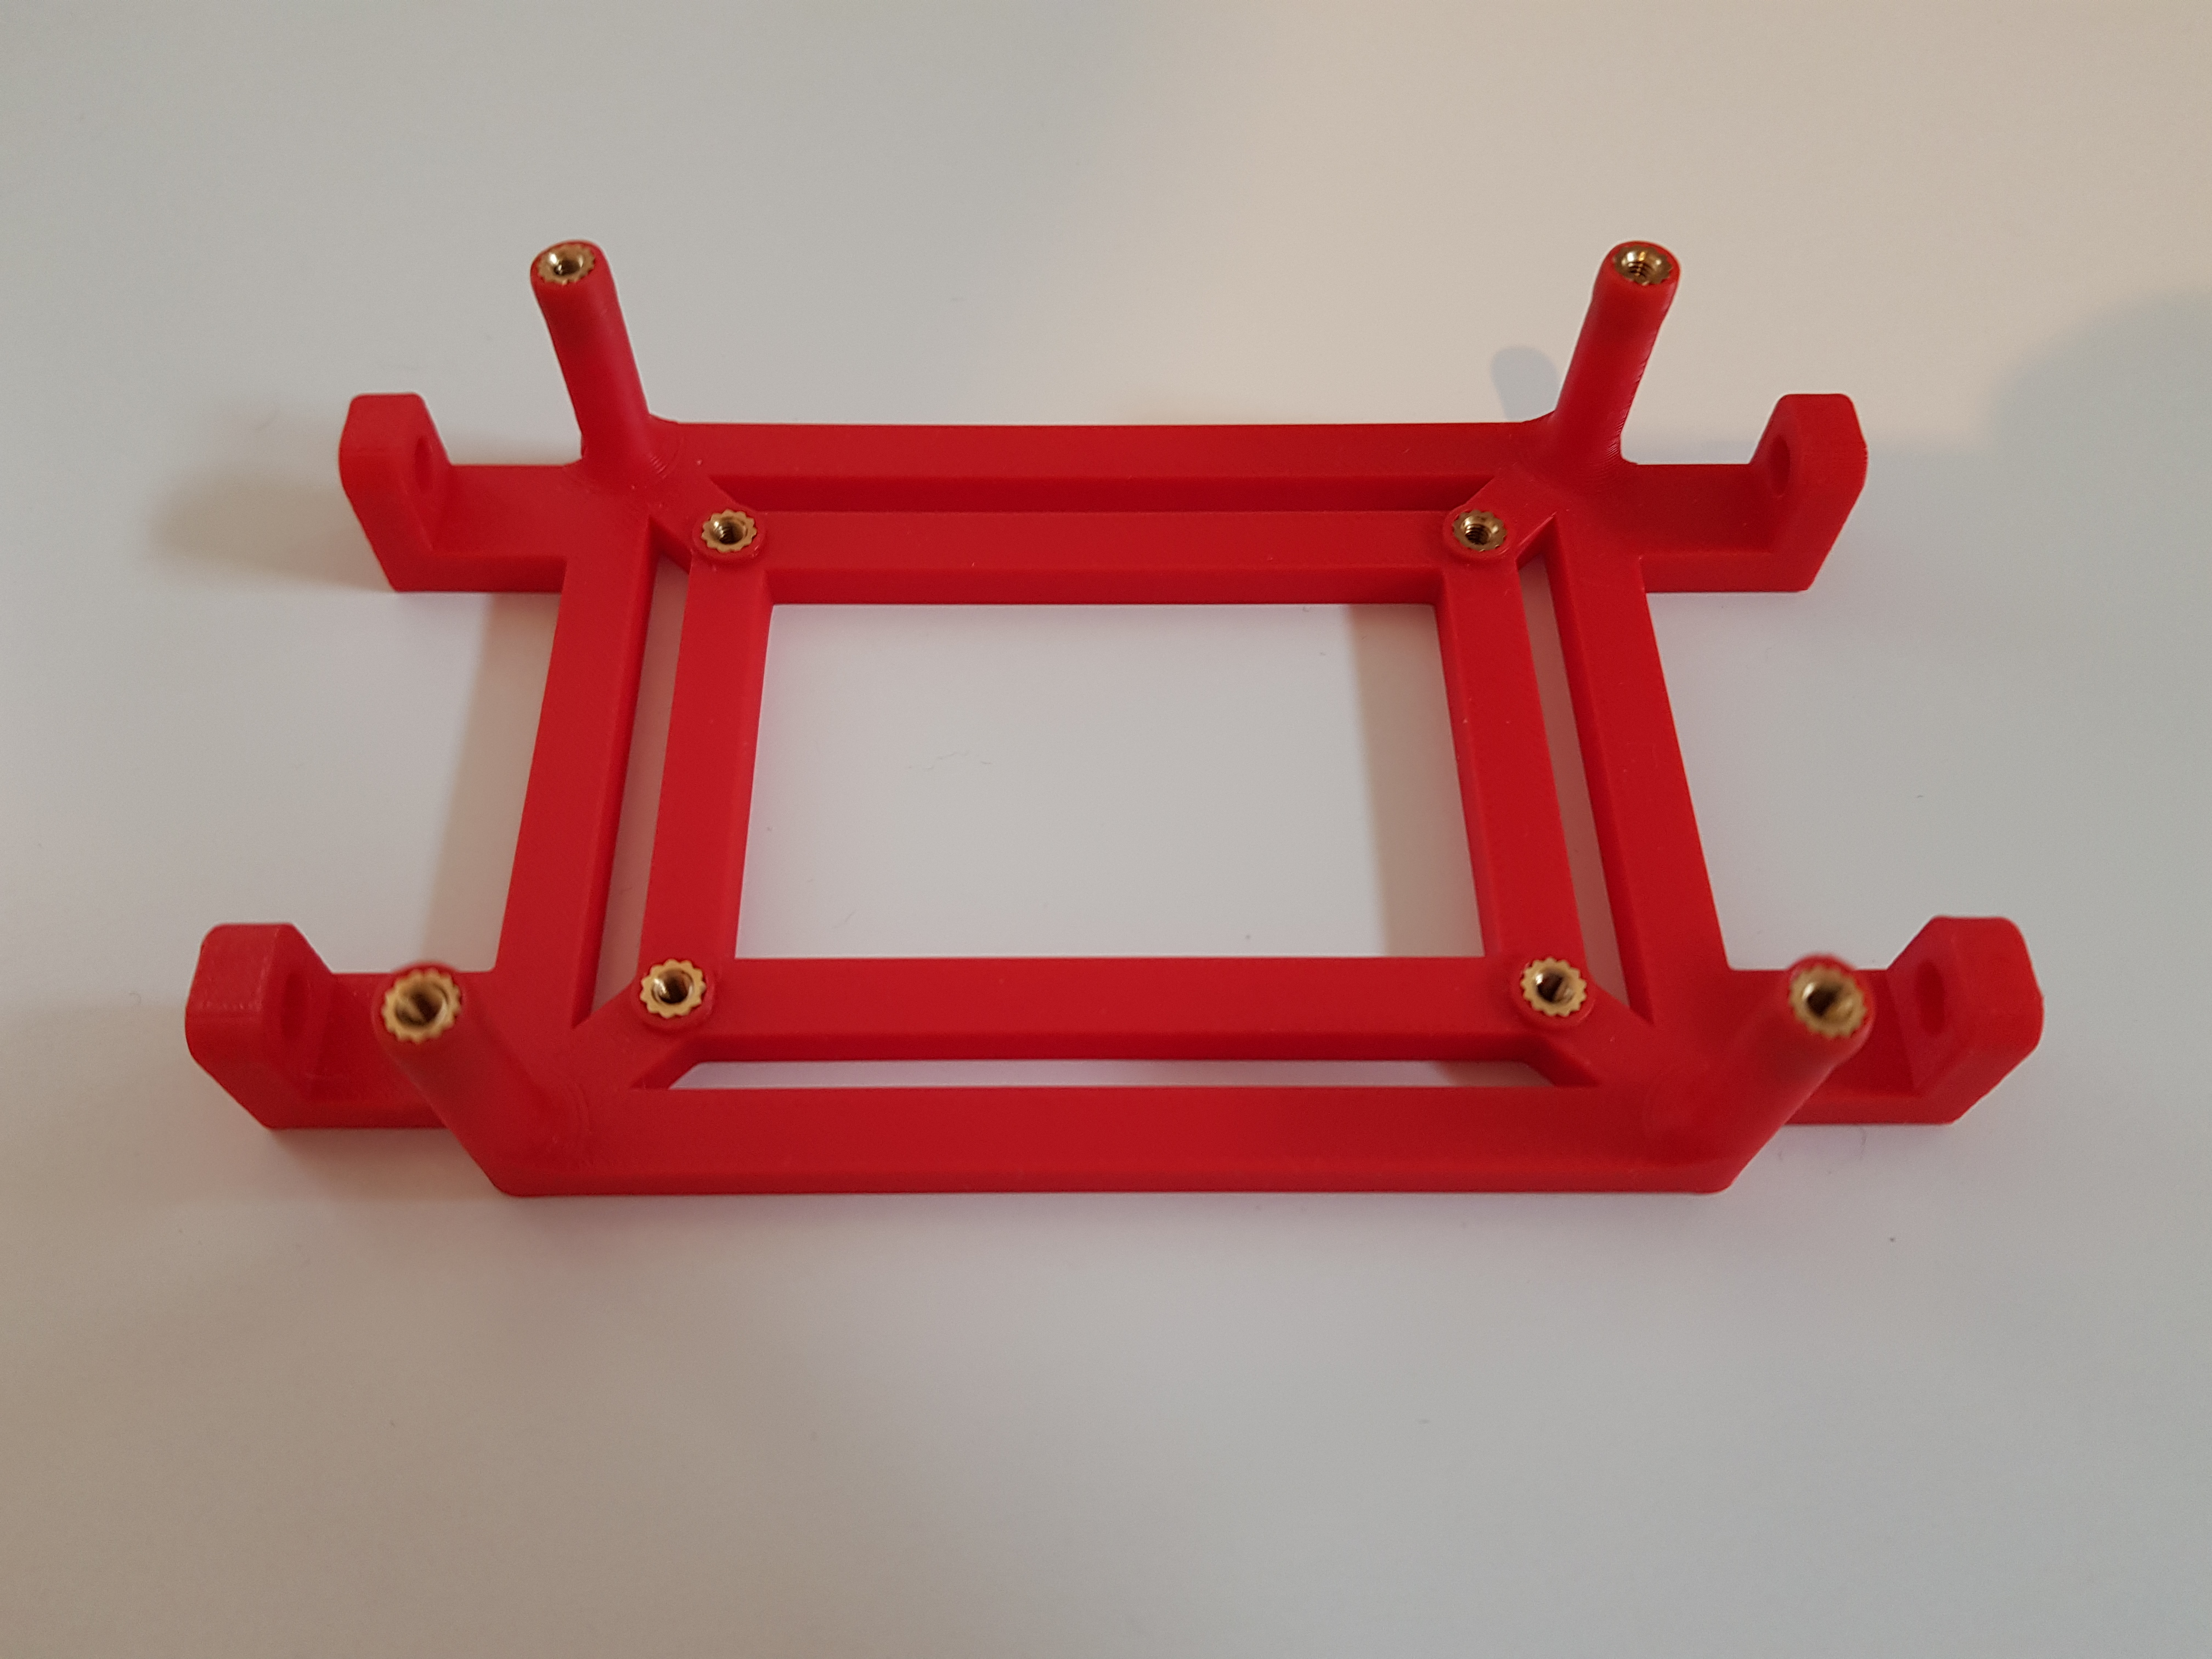
\includegraphics[height=0.7\textwidth]{board_mounting_rack_thread_inserts}
		\caption{Board mounting rack thread inserts}
		\label{fig:boardmountingrackthreadinserts}
	\end{subfigure}
	\caption{Thread inserts}
	\label{fig:Thread inserts}
\end{figure}

The thread inserts were inserted into the chassis using a soldering iron as shown in figure \ref{fig:Thread inserts} for the body, knee wheel links and board mounting rack.
Minimum force was applied to the soldering iron to align the thread inserts surface with the surface of the chassis.
%two subfigures for mounting the motors on the knee wheel links
\begin{figure}[h]
	\centering
	\begin{subfigure}[t]{0.45\textwidth}
		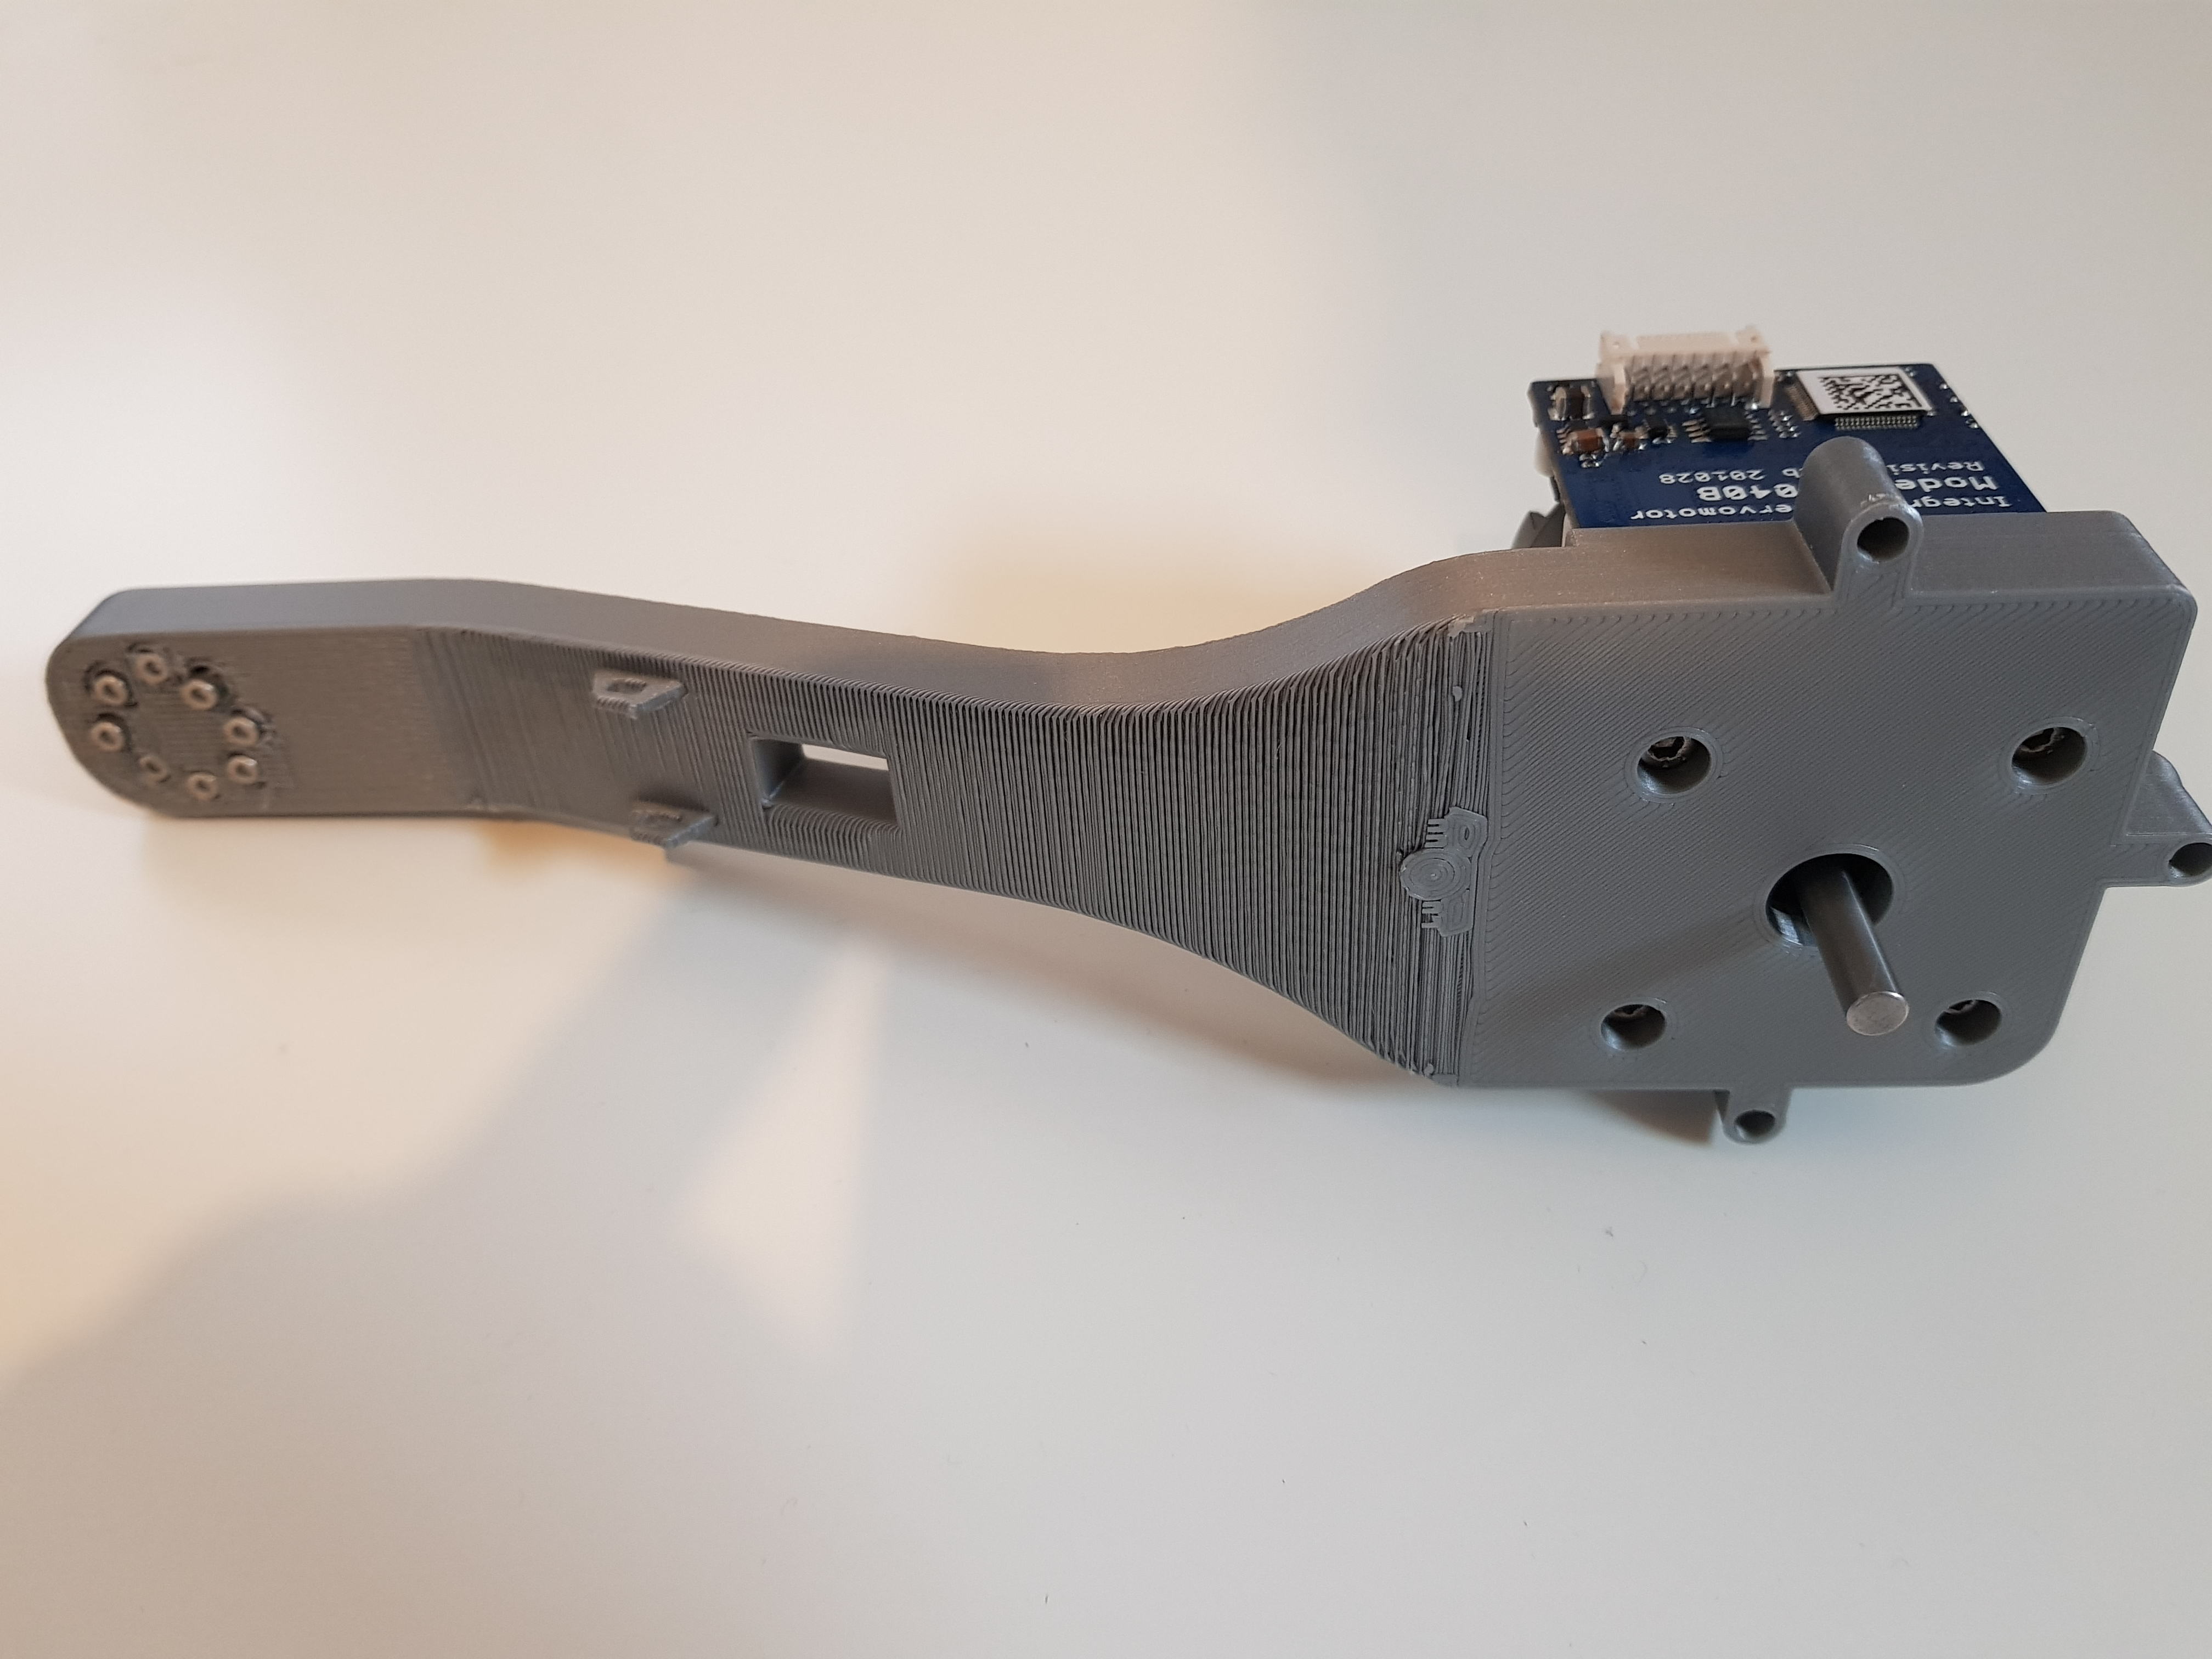
\includegraphics[height=0.7\textwidth]{mounting_motors_on_knee_wheel_links_1}
		\caption{Mounting motors on knee wheel links perspective view}
		\label{fig:mountingmotorsonkneewheellinksperpectiveview}
	\end{subfigure}
	\begin{subfigure}[t]{0.45\textwidth}
		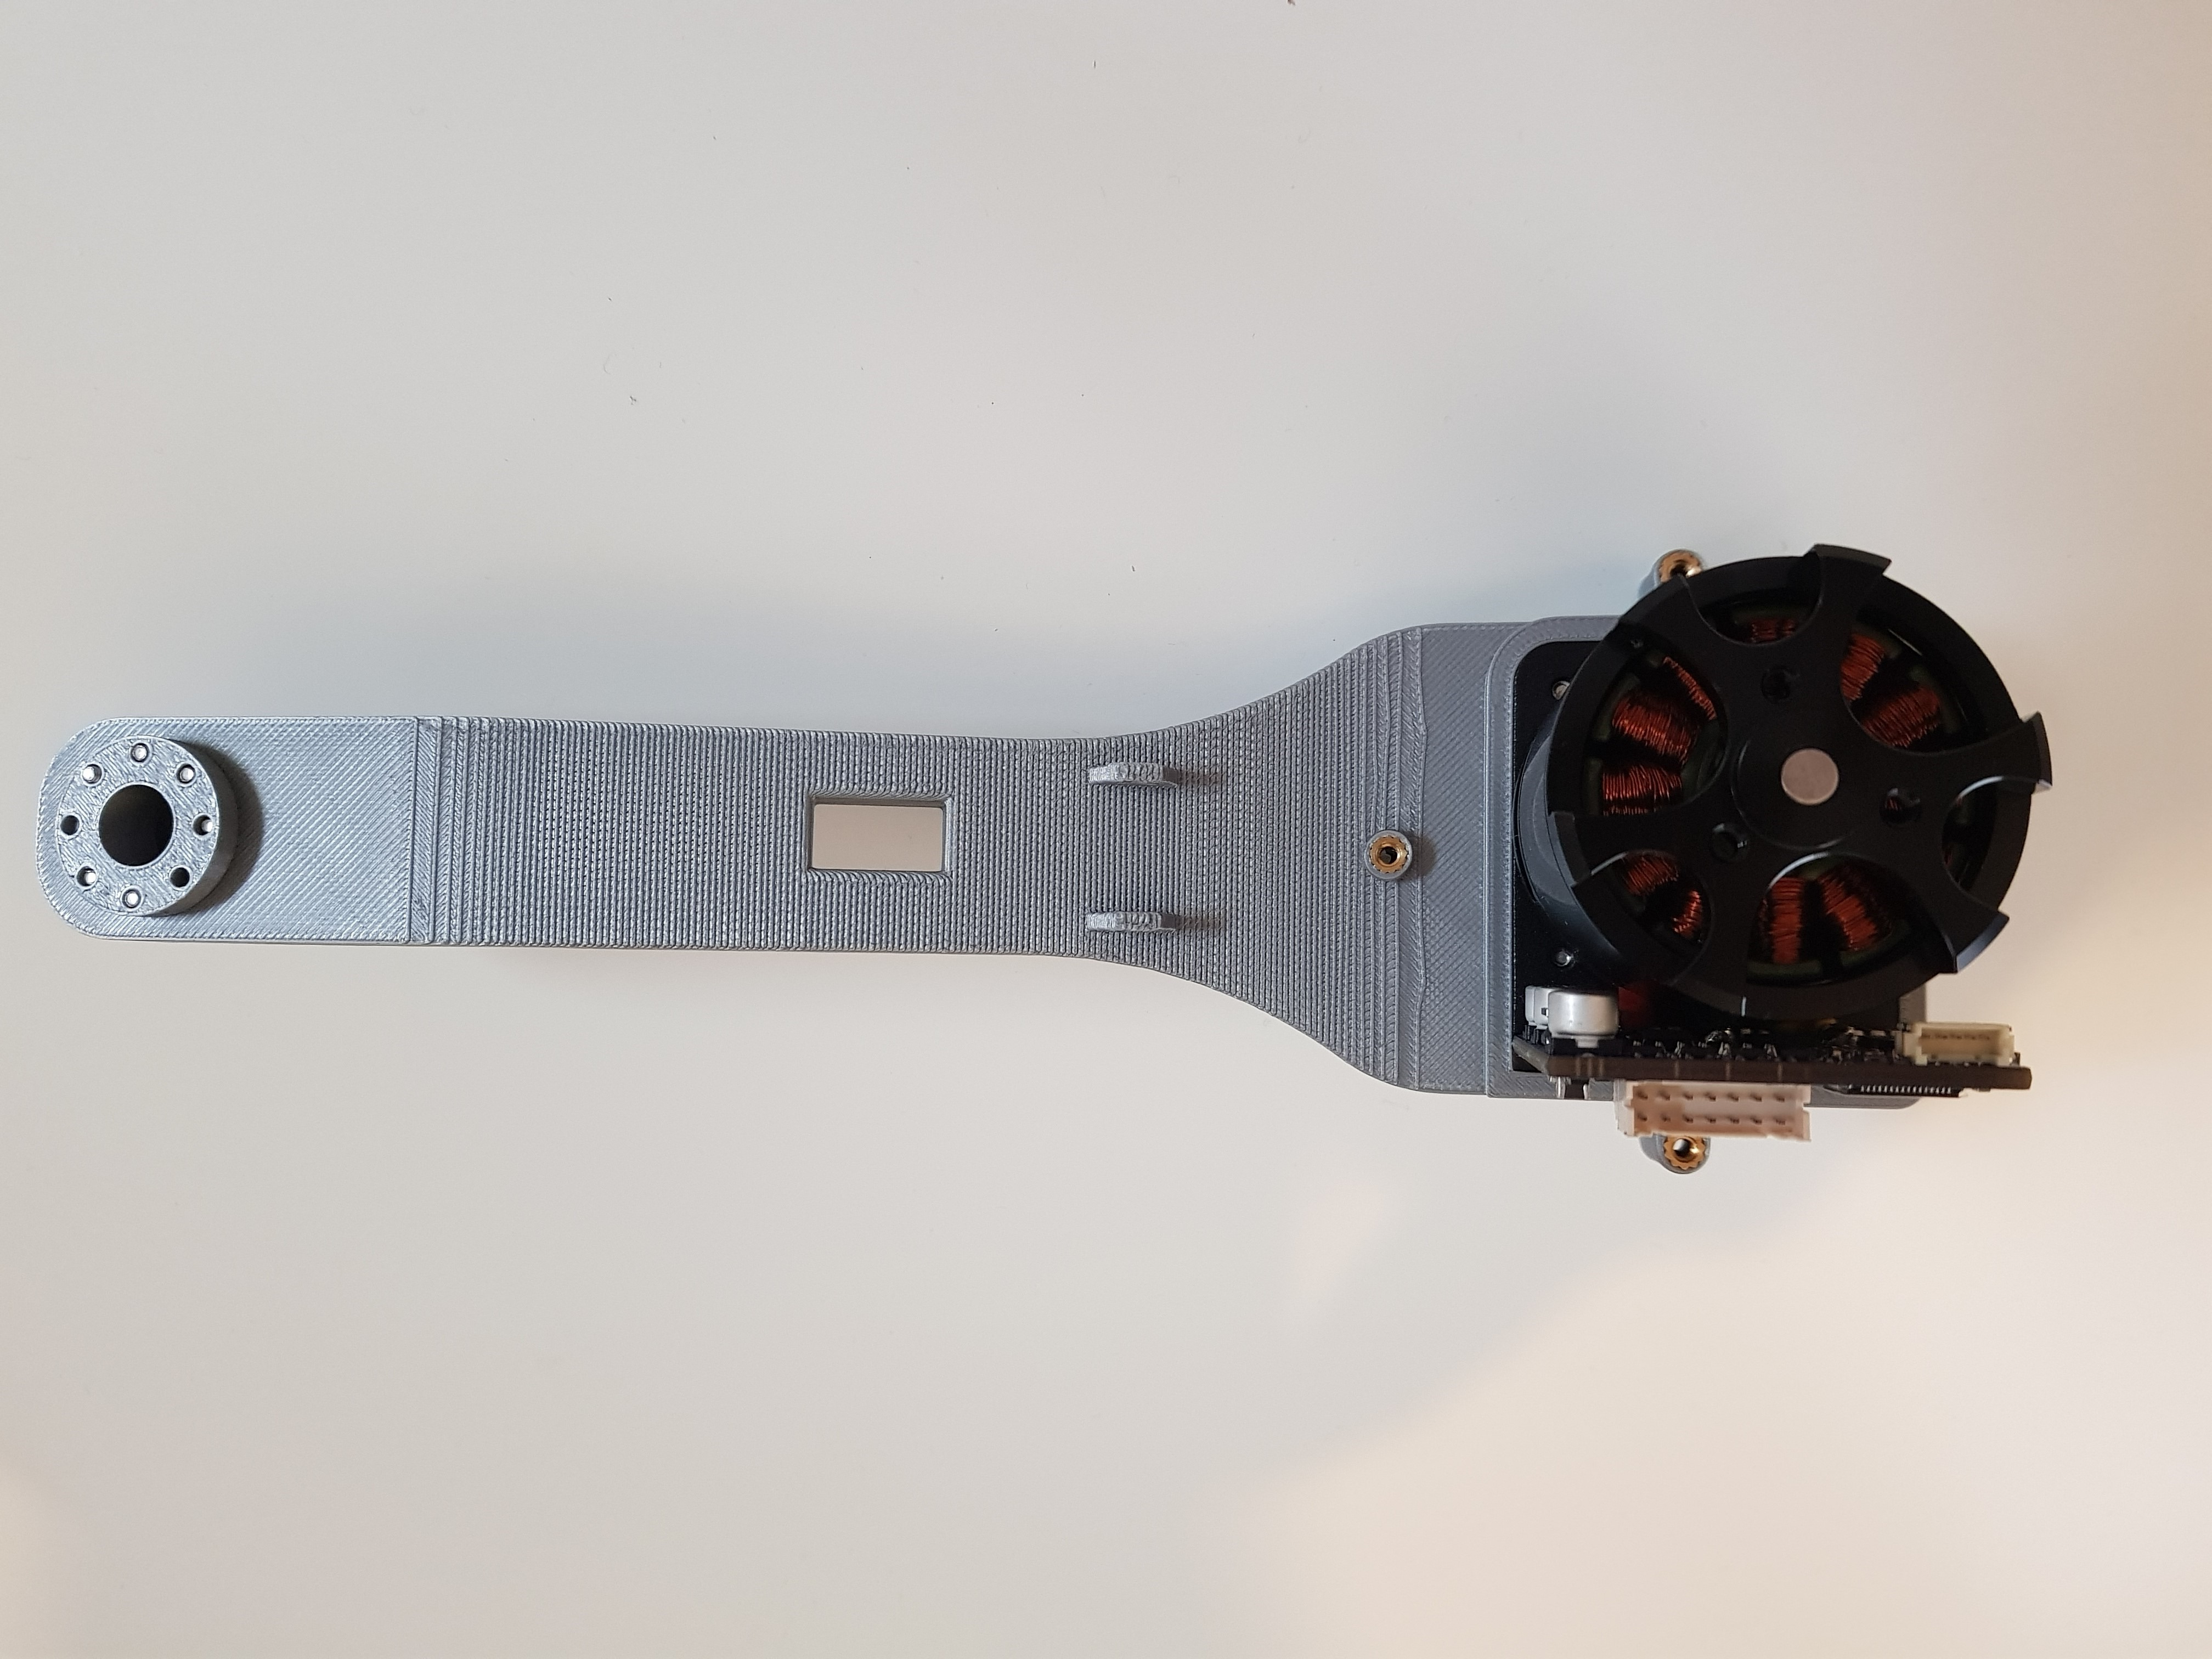
\includegraphics[height=0.7\textwidth]{mounting_motors_on_knee_wheel_links_2}
		\caption{Mounting motors on knee wheel links top view}
		\label{fig:mountingmotorsonkneewheellinkstopview}
	\end{subfigure}
	\caption{Mounting motors on knee wheel links}
	\label{fig:Mounting motors on knee wheel links}
\end{figure}
%%figure for mounting the motors on the knee wheel links
%\begin{figure}[h]
%	\centering
%	\includegraphics[width=0.5\linewidth]{mounting_motors_on_knee_wheel_links}
%	\caption{Mounting motors on knee wheel links}
%	\label{fig:mountingmotorsonkneewheellinks}
%\end{figure}
The motors were mounted on the knee wheel links using four screws, as shown in figure \ref{fig:mountingmotorsonkneewheellinks}.
%two subfigures for mounting the motors on the hip knee links
\begin{figure}[h]
	\centering
	\begin{subfigure}[t]{0.45\textwidth}
		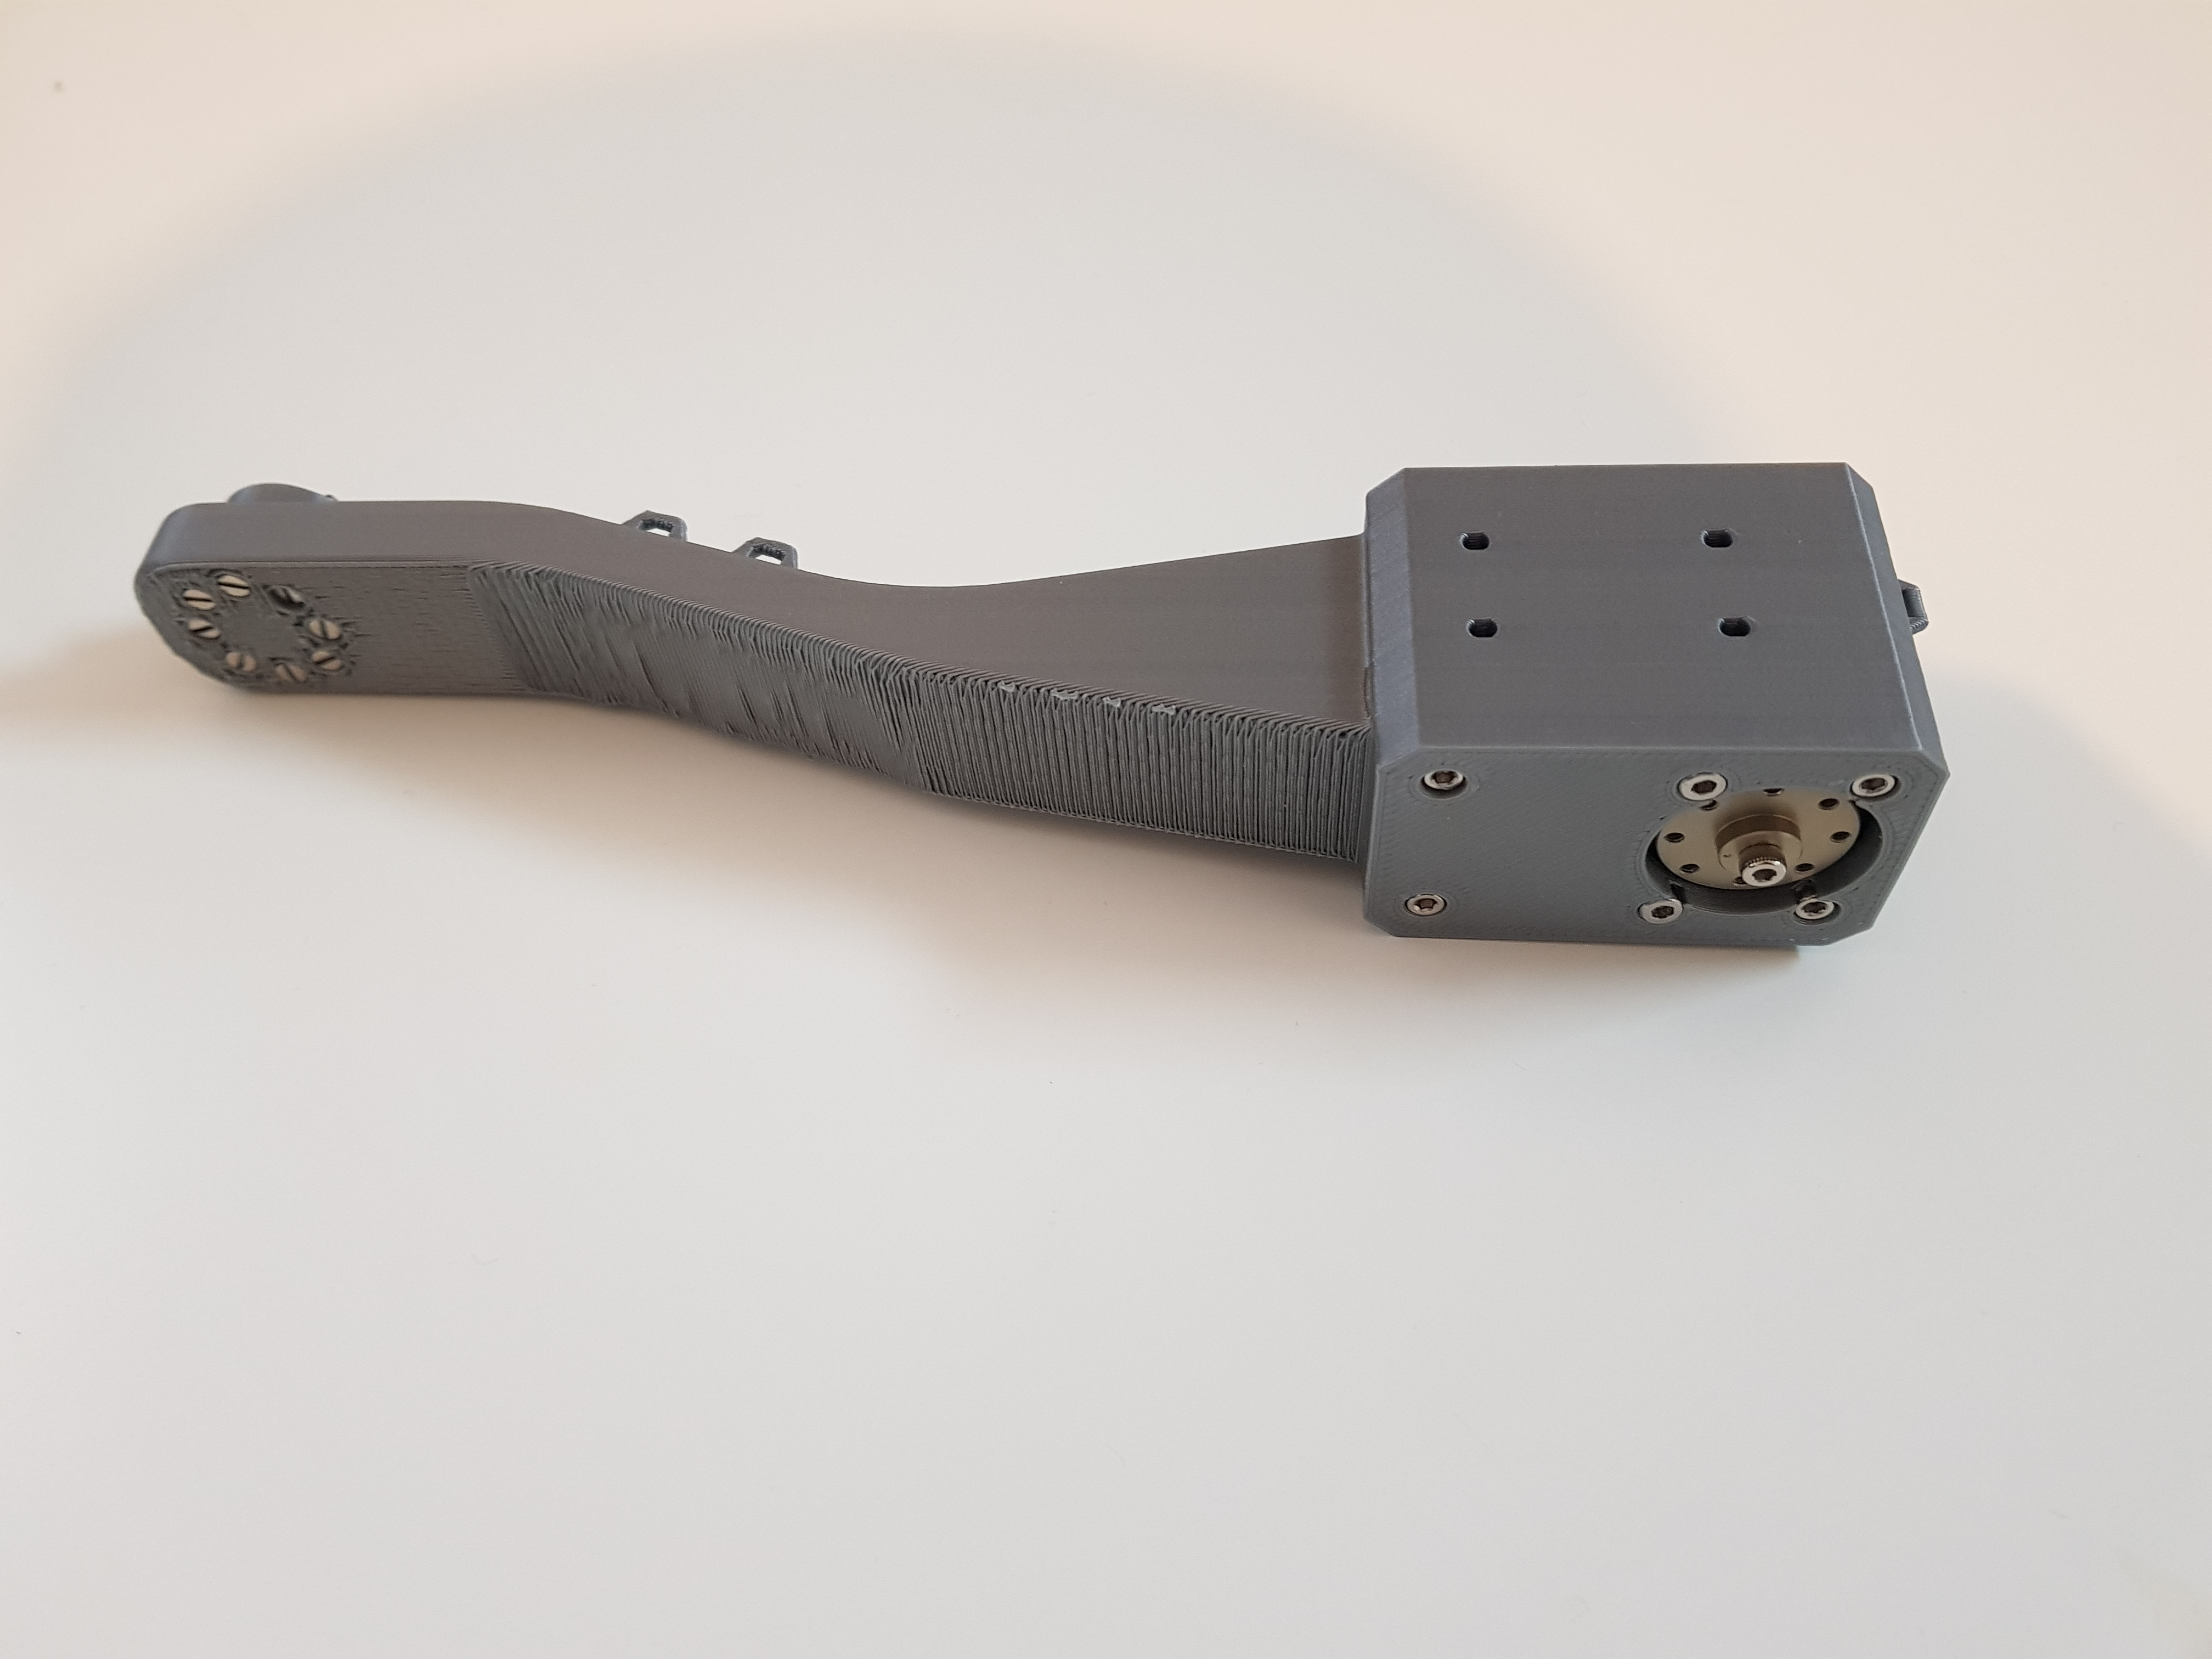
\includegraphics[height=0.7\textwidth]{mounting_motors_on_hip_knee_links_1}
		\caption{Mounting motors on hip knee links perspective view}
		\label{fig:mountingmotorsonhipkneelinksperspectiveview}
	\end{subfigure}
	\begin{subfigure}[t]{0.45\textwidth}
		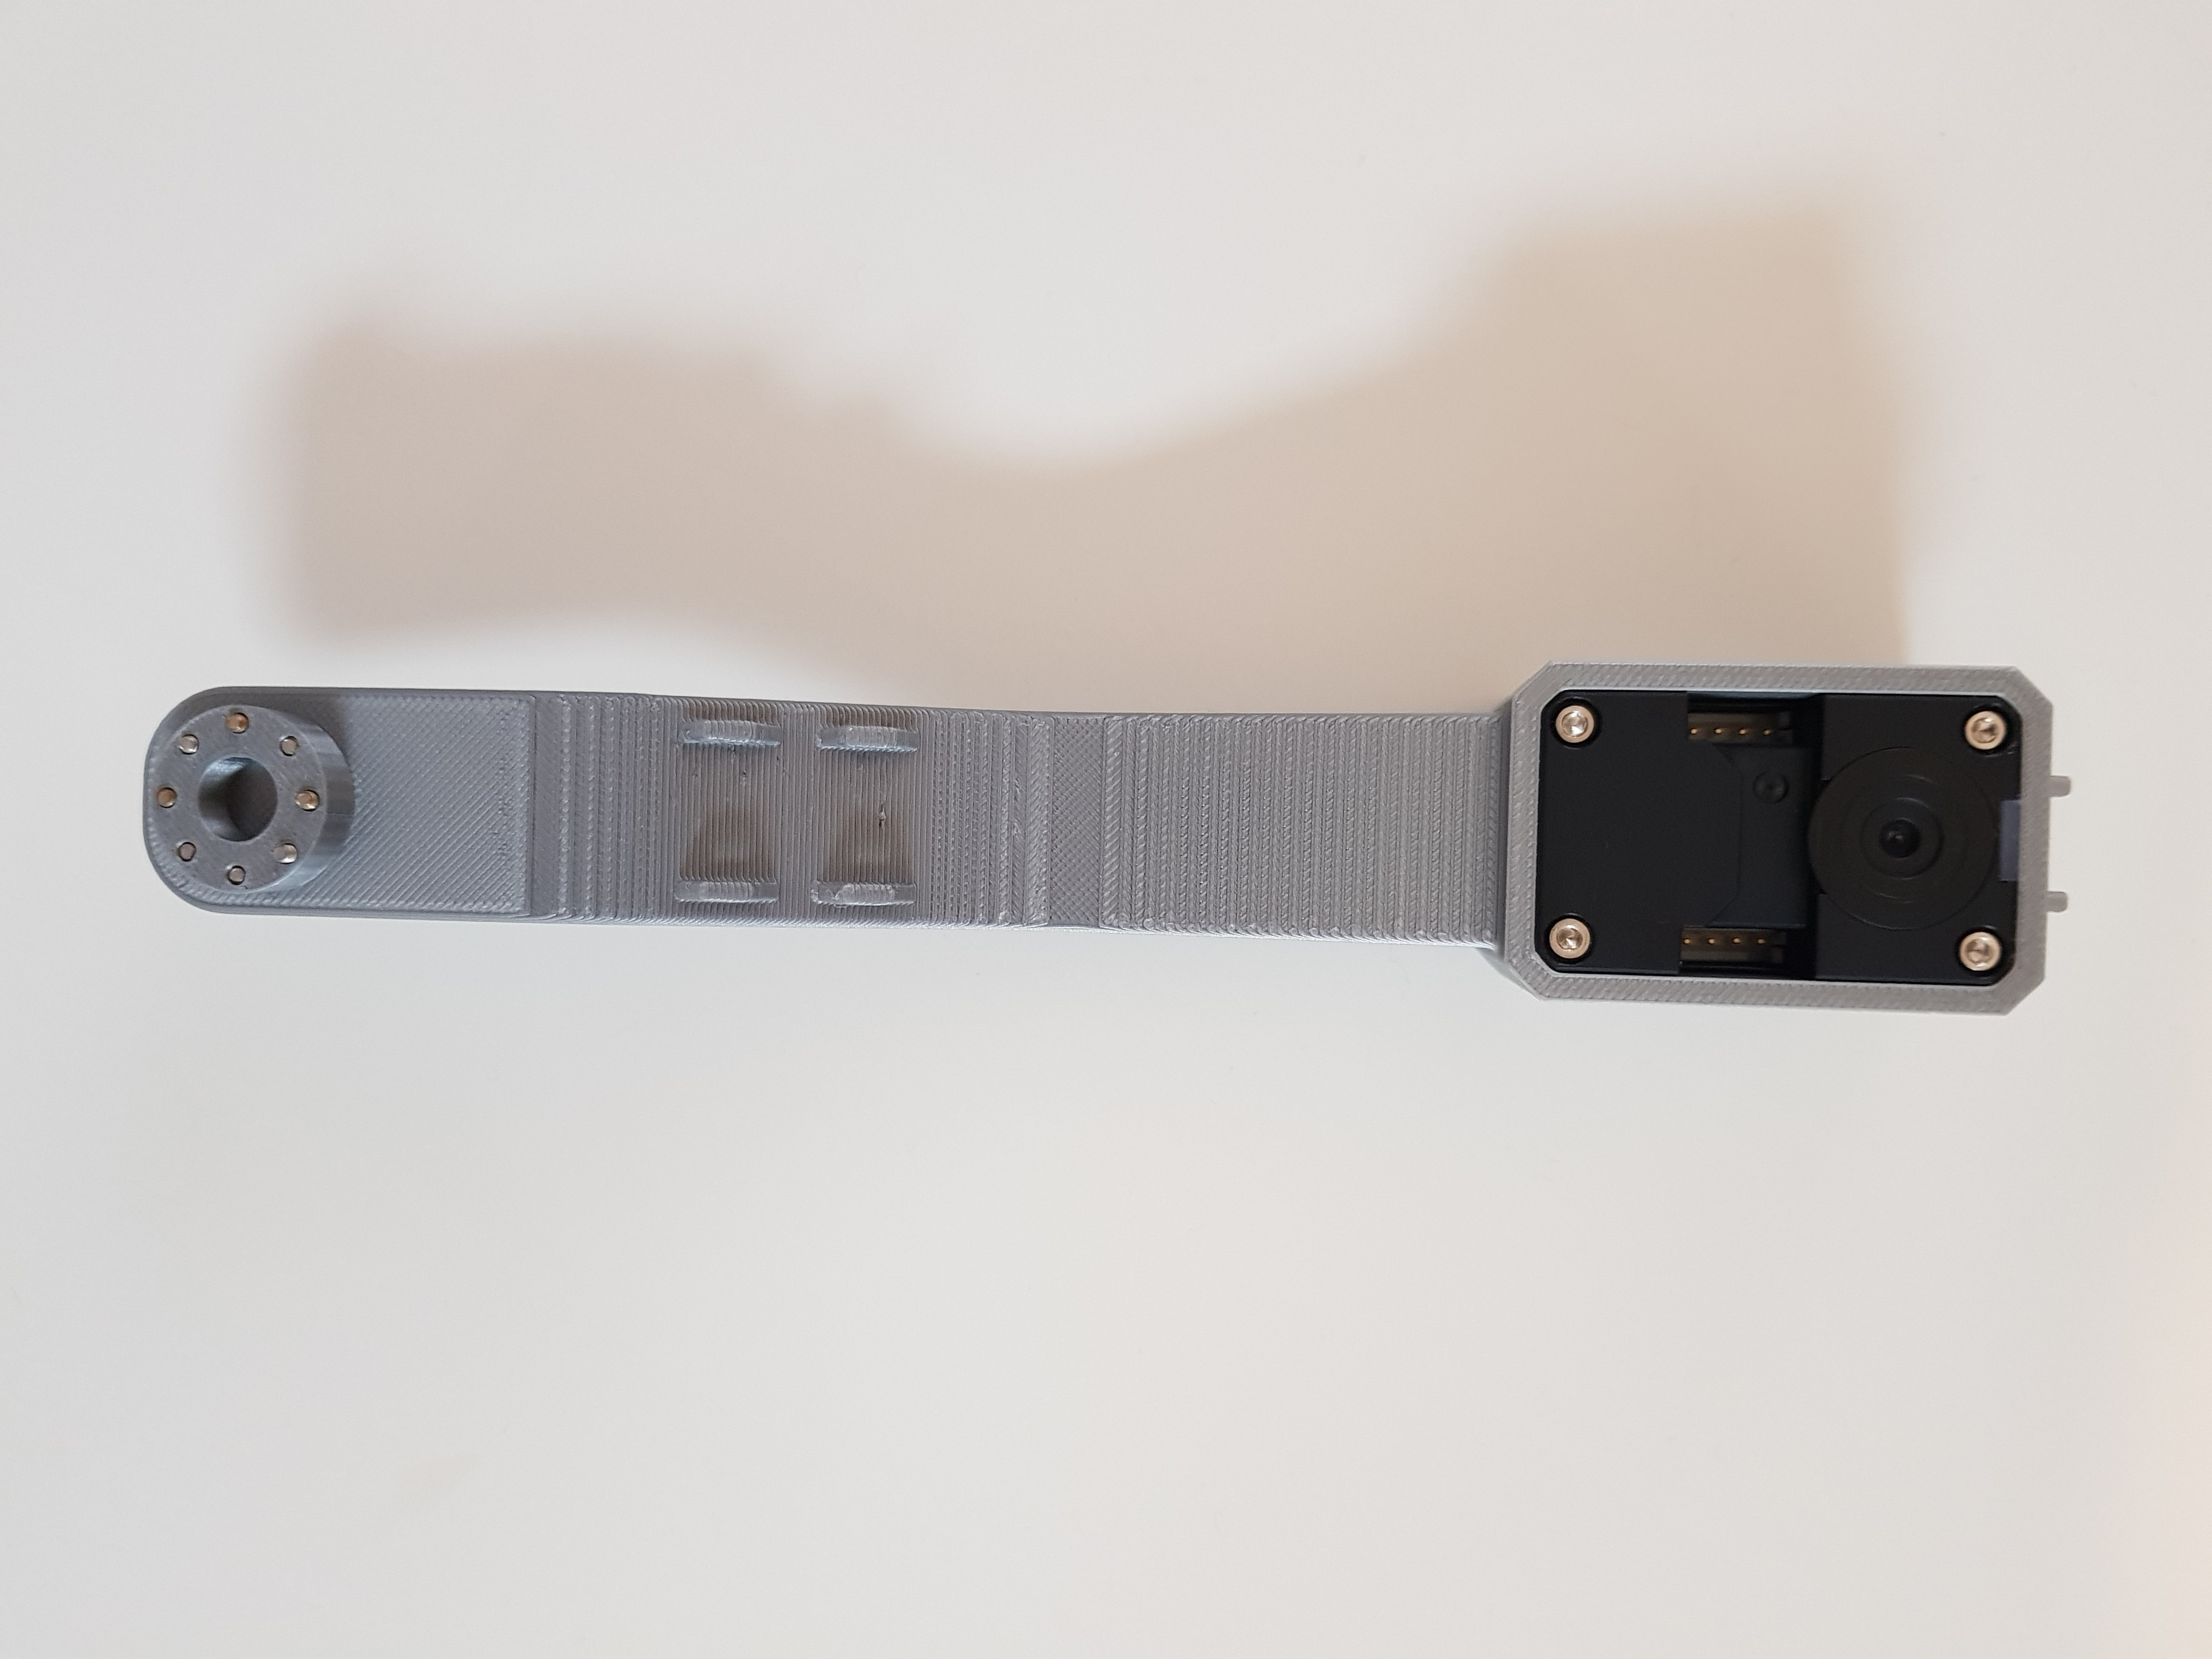
\includegraphics[height=0.7\textwidth]{mounting_motors_on_hip_knee_links_2}
		\caption{Mounting motors on hip knee links top view}
		\label{fig:mountingmotorsonhipkneelinkstopview}
	\end{subfigure}
	\caption{Mounting motors on hip knee links}
	\label{fig:Mounting motors on hip knee links}
\end{figure}
%%figure for mounting the motors on the hip knee links
%\begin{figure}[h]
%	\centering
%	\includegraphics[width=0.5\linewidth]{mounting_motors_on_hip_knee_links}
%	\caption{Mounting motors on hip knee links}
%	\label{fig:mountingmotorsonhipkneelinks}
%\end{figure}
%two subfigures for assembling the knee wheel links and hip knee links
\begin{figure}[h]
	\centering
	\begin{subfigure}[t]{0.45\textwidth}
		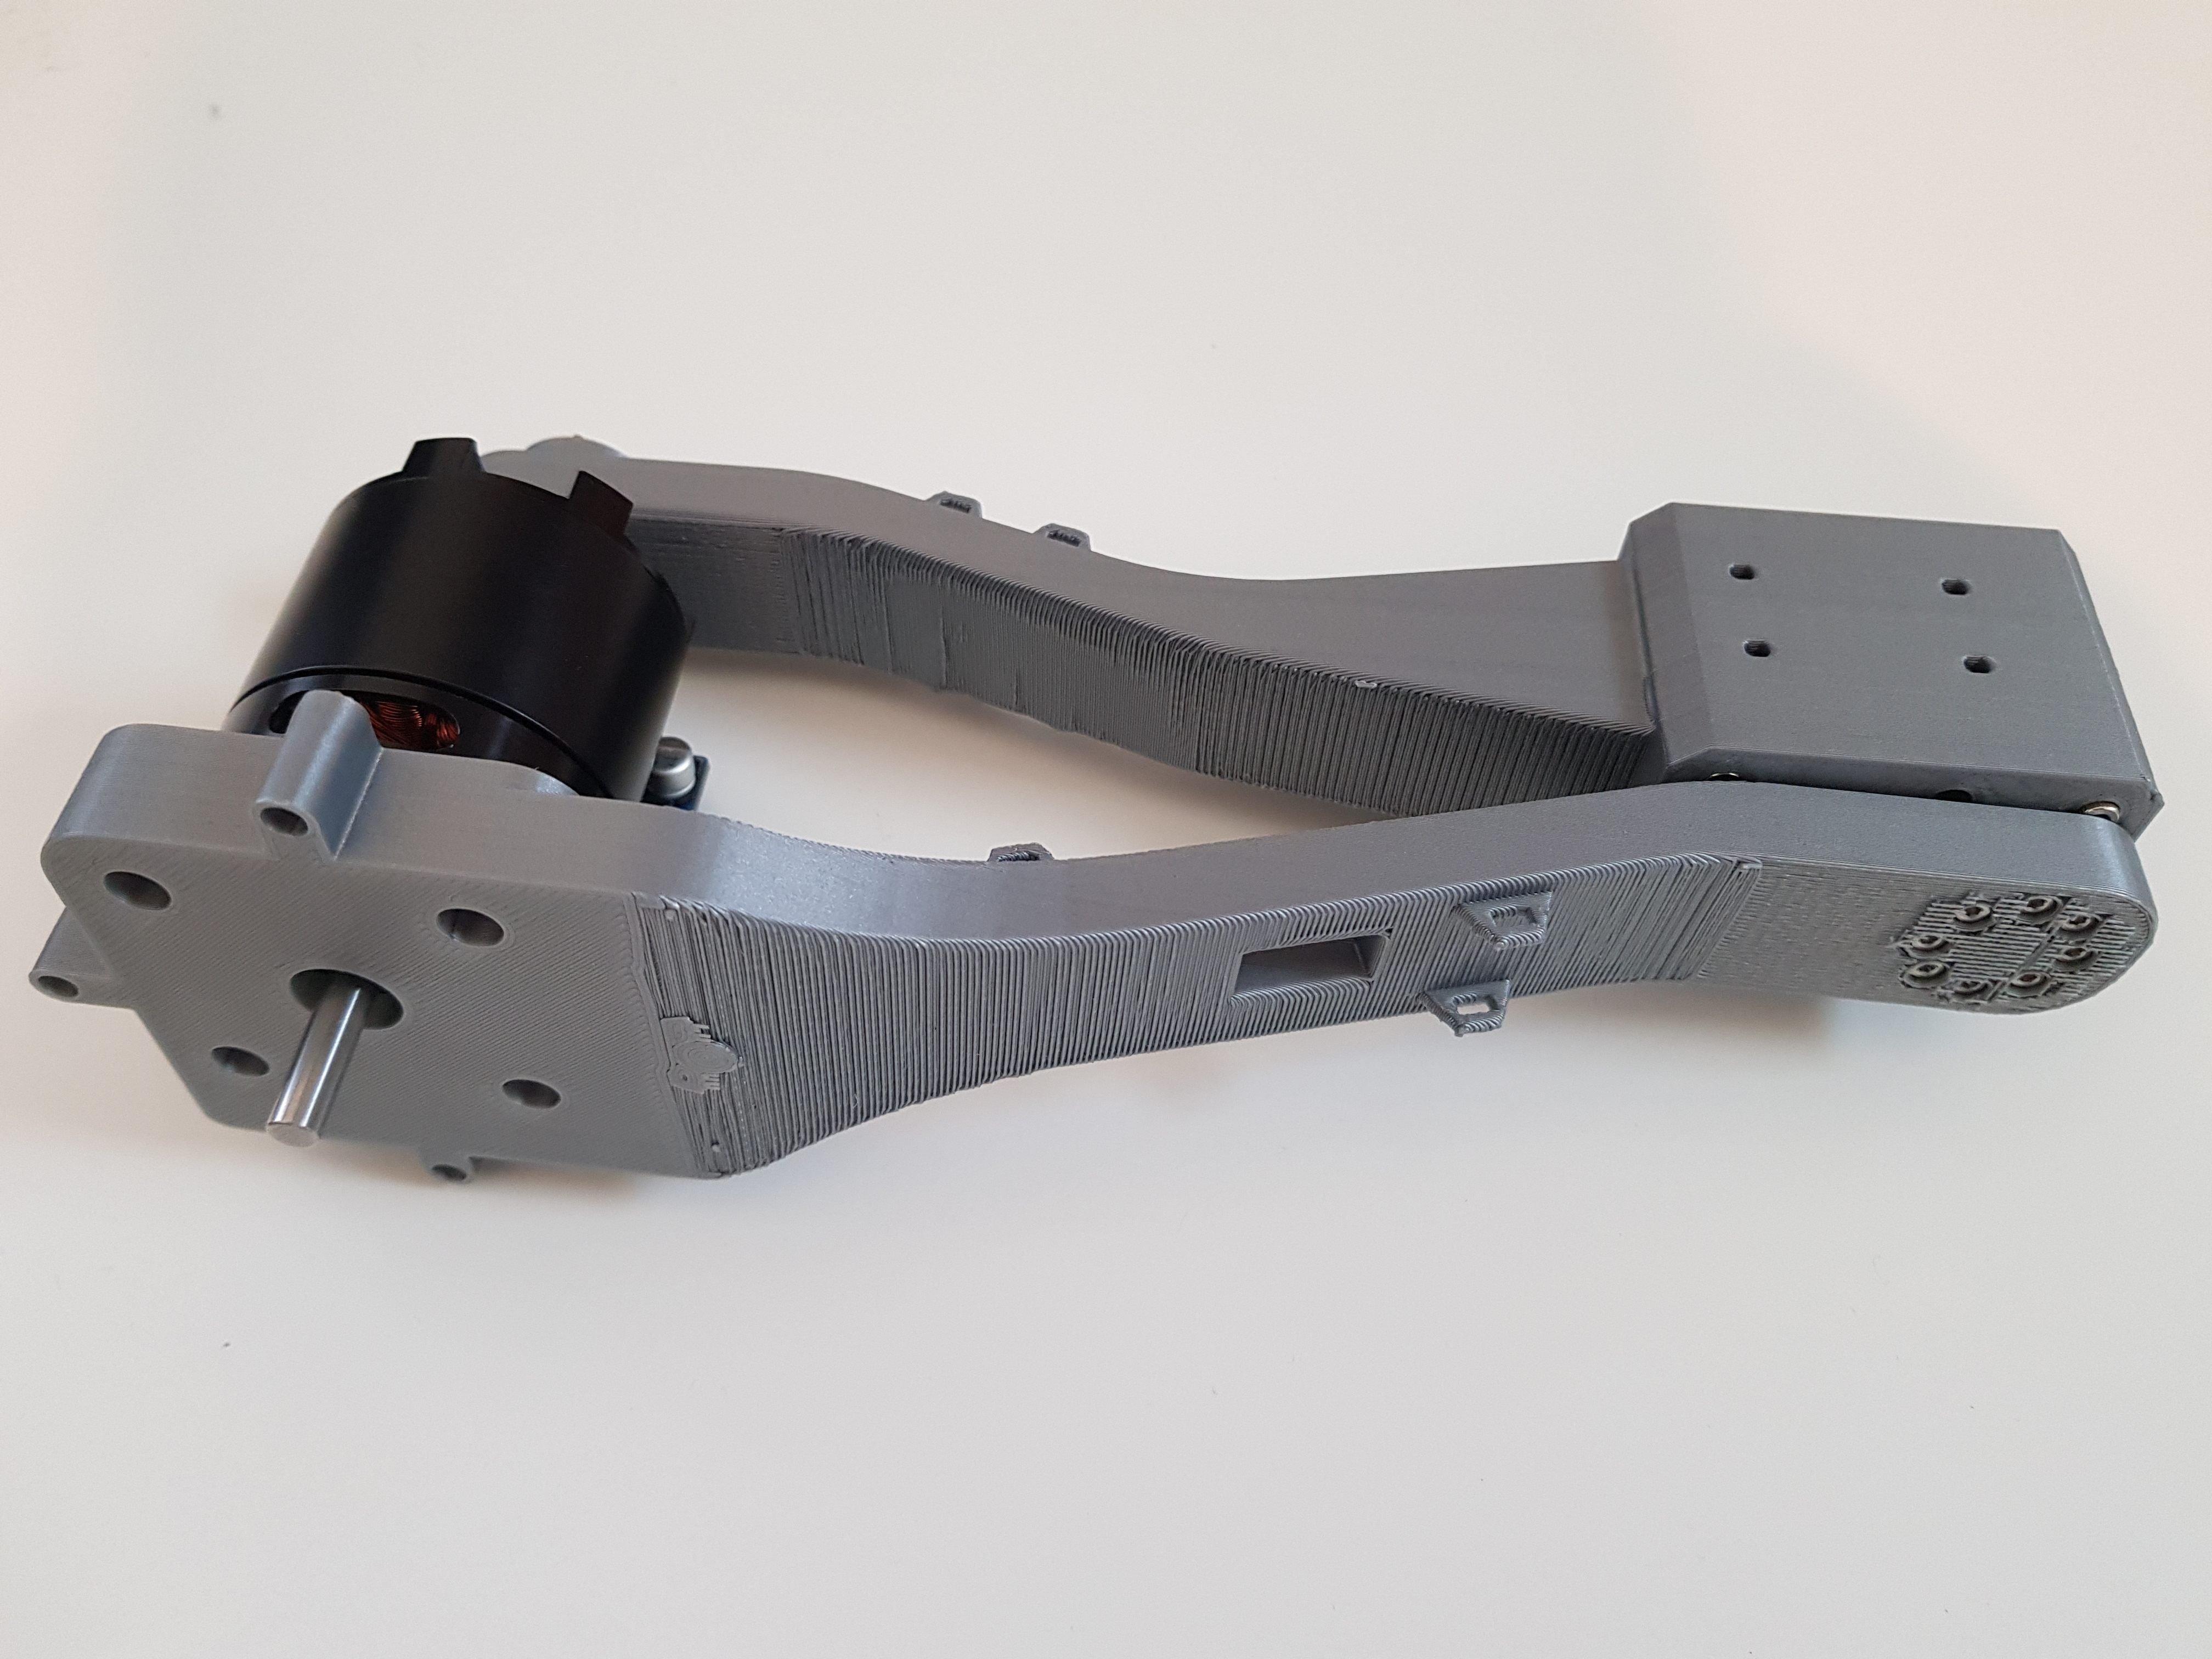
\includegraphics[height=0.7\textwidth]{assembling_knee_wheel_links_and_hip_knee_links_1}
		\caption{Assembling knee wheel links and hip knee links	prespective view}
		\label{fig:assemblingkneewheellinksandhipkneelinksprespectiveview}
	\end{subfigure}
	\begin{subfigure}[t]{0.45\textwidth}
		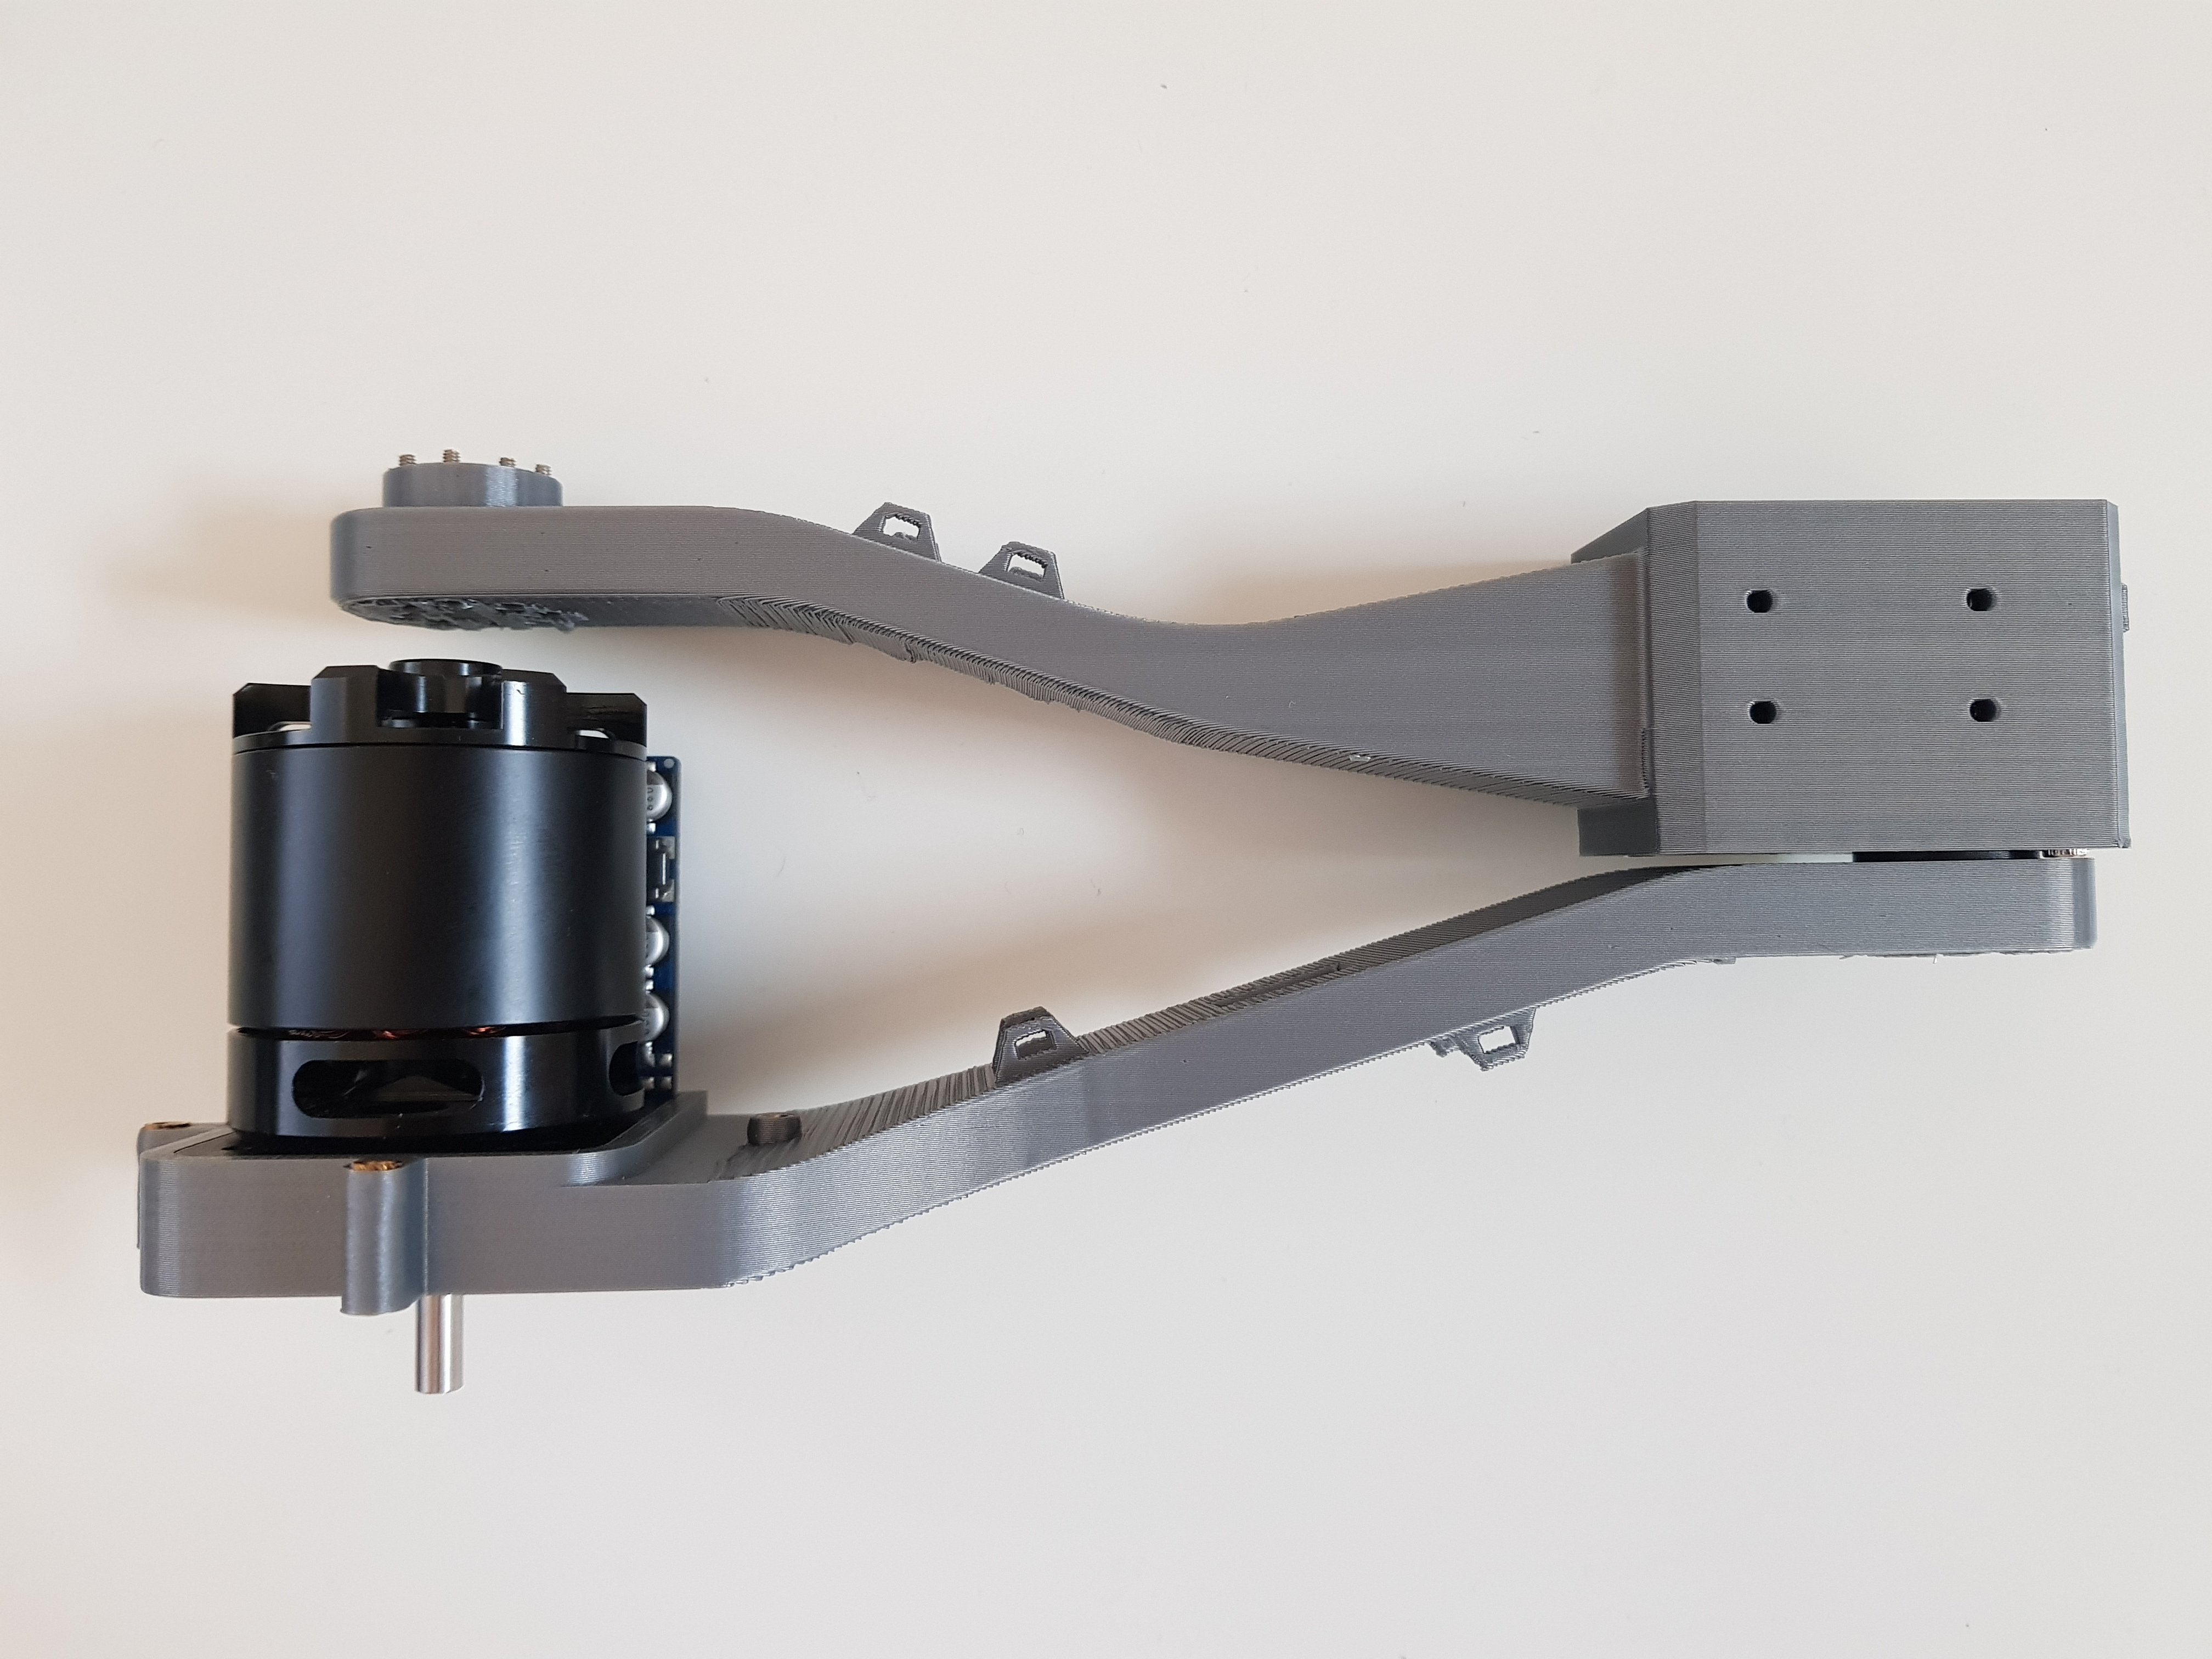
\includegraphics[height=0.7\textwidth]{assembling_knee_wheel_links_and_hip_knee_links_2}
		\caption{Assembling knee wheel links and hip knee links	top view}
		\label{fig:assemblingkneewheellinksandhipkneelinkstopview}
	\end{subfigure}
	\caption{Assembling knee wheel links and hip knee links}
	\label{fig:Assembling knee wheel links and hip knee links}
\end{figure}

%%figure for assembled knee wheel links and hip knee links
%\begin{figure}[h]
%	\centering
%	\includegraphics[width=0.5\linewidth]{assembled_knee_wheel_links_and_hip_knee_links}
%	\caption{Assembled knee wheel links and hip knee links}
%	\label{fig:assembledkneewheellinksandhipkneelinks}
%\end{figure}
%figure for the assembing the body hip knee links.
\newpage
\begin{figure}[h]
	\centering
	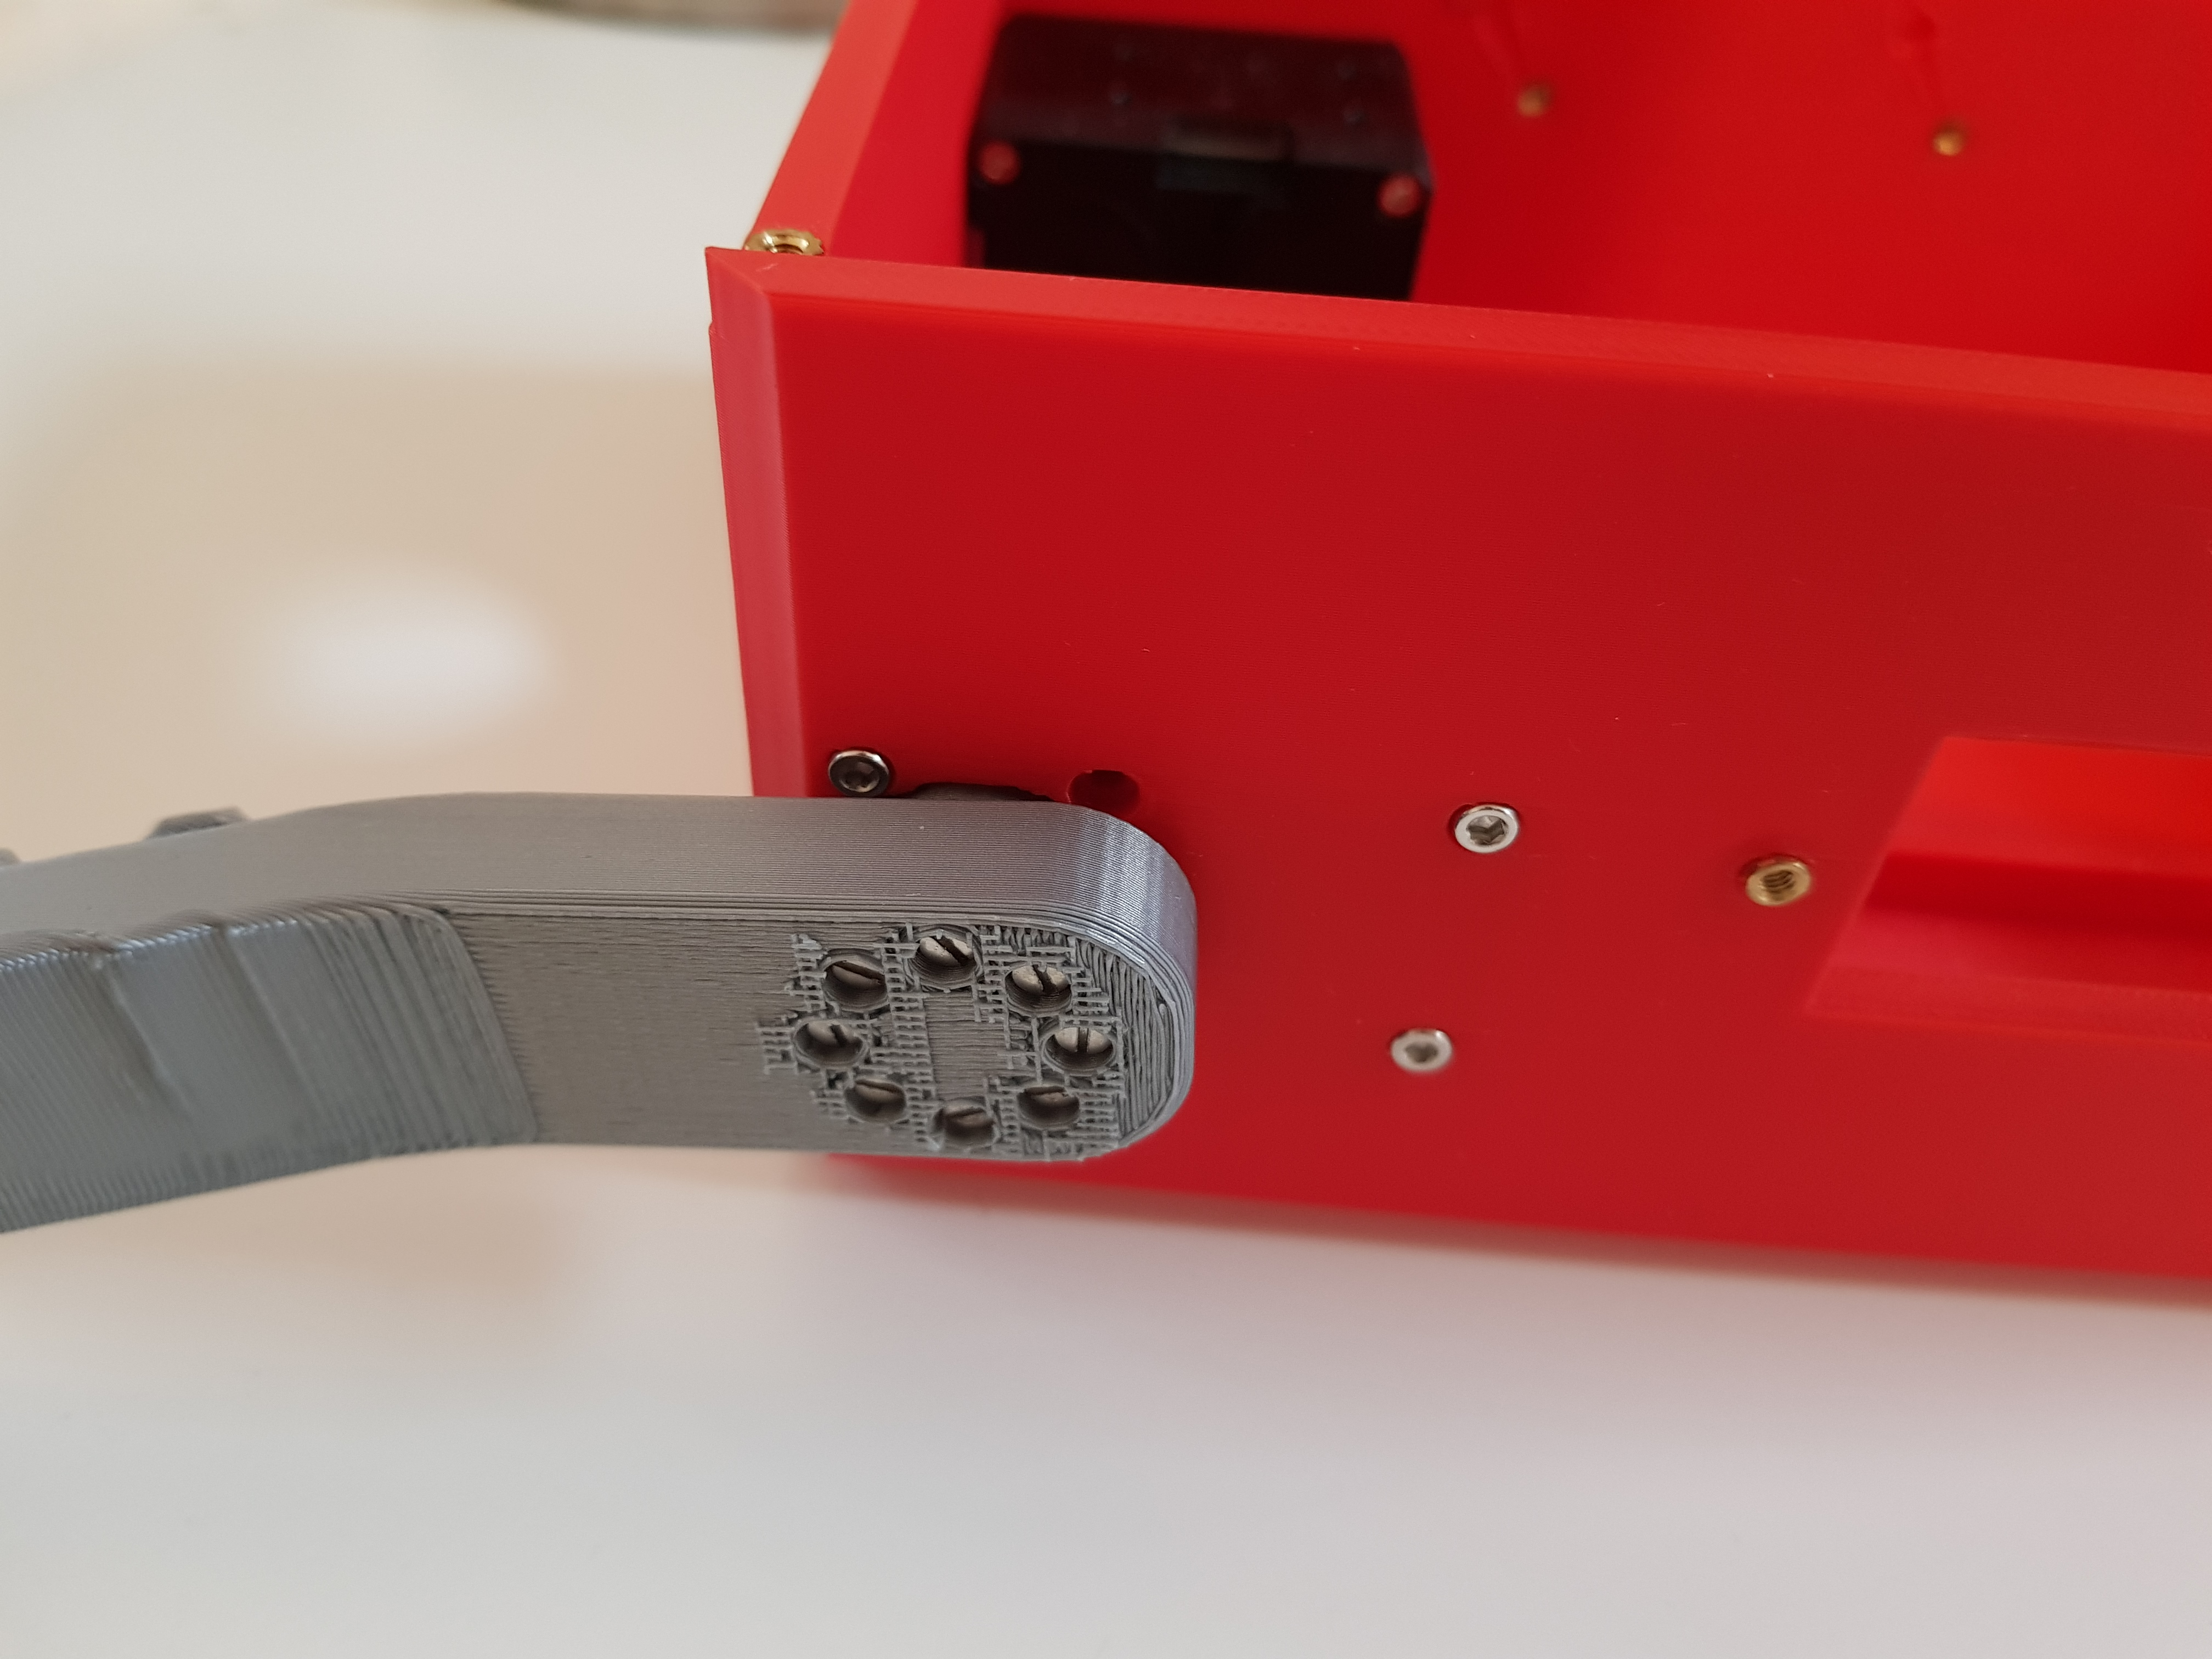
\includegraphics[width=0.5\linewidth]{assembling_body_hip_knee_links}
	\caption{Assembling body to hip knee links}
	\label{fig:assemblingbodyhipkneelinks}
\end{figure}
The hip knee links were assembled to the body using sixteen screws as shown in figure \ref{fig:assemblingbodyhipkneelinks} to the hip motor horns after the motors were mounted in the body.
%figure for fully assembled chassis
\begin{figure}[h]
	\centering
	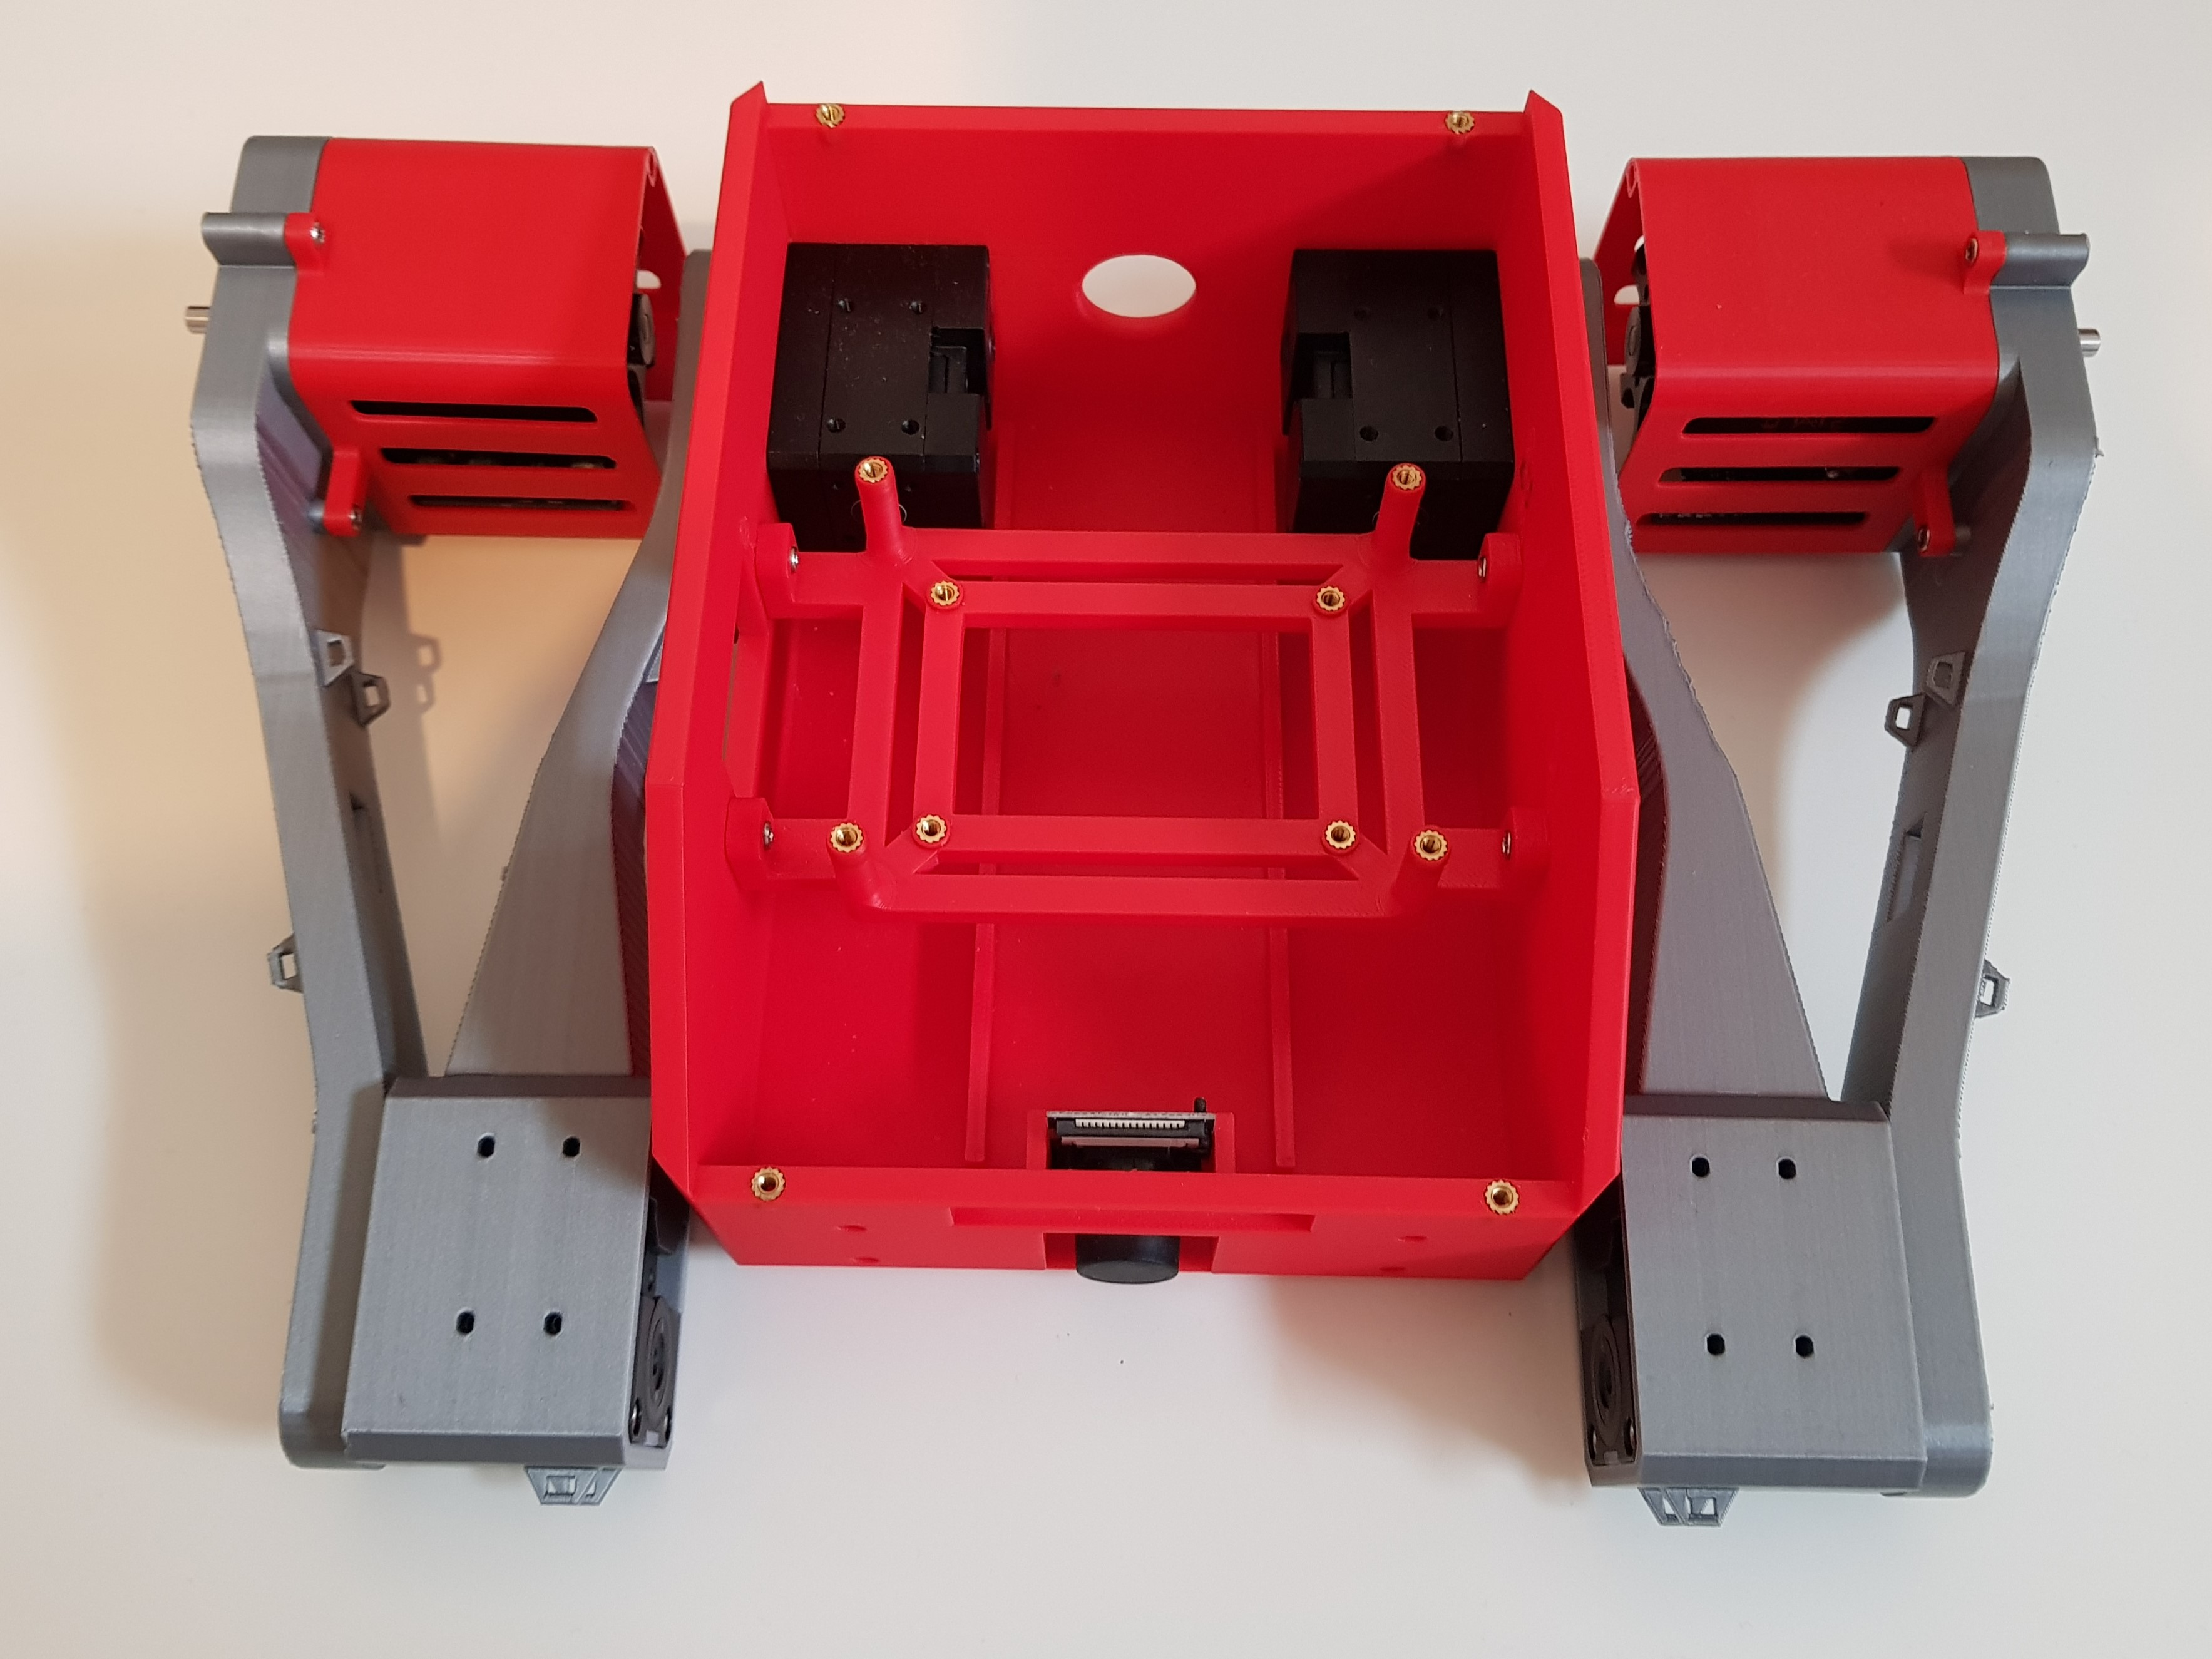
\includegraphics[width=0.5\linewidth]{fully_assembled_chassis}
	\caption{Fully assembled chassis}
	\label{fig:fullyassembledchassis}
\end{figure}

\section{Integration of Mechanical and Electronic Systems}

%how the electronics were mounted on the chassis

\subsection{Wiring tree}
%how the wiring was made
According to the wiring tree in the electrical design chapter, the wiring tree was made to fit the lengthes between the components.
%figure for the wiring tree
%\begin{figure}[h]
%%	\centering
%%	\includegraphics[width=0.5\linewidth]{wiring_tree}
%%	\caption{Wiring tree}
%%	\label{fig:wiringtree}
%%\end{figure}
%

\subsection{Electronics Assembly}
%figure for the electronics mounted on the board mounting rack
\begin{figure}[h]
	\centering
	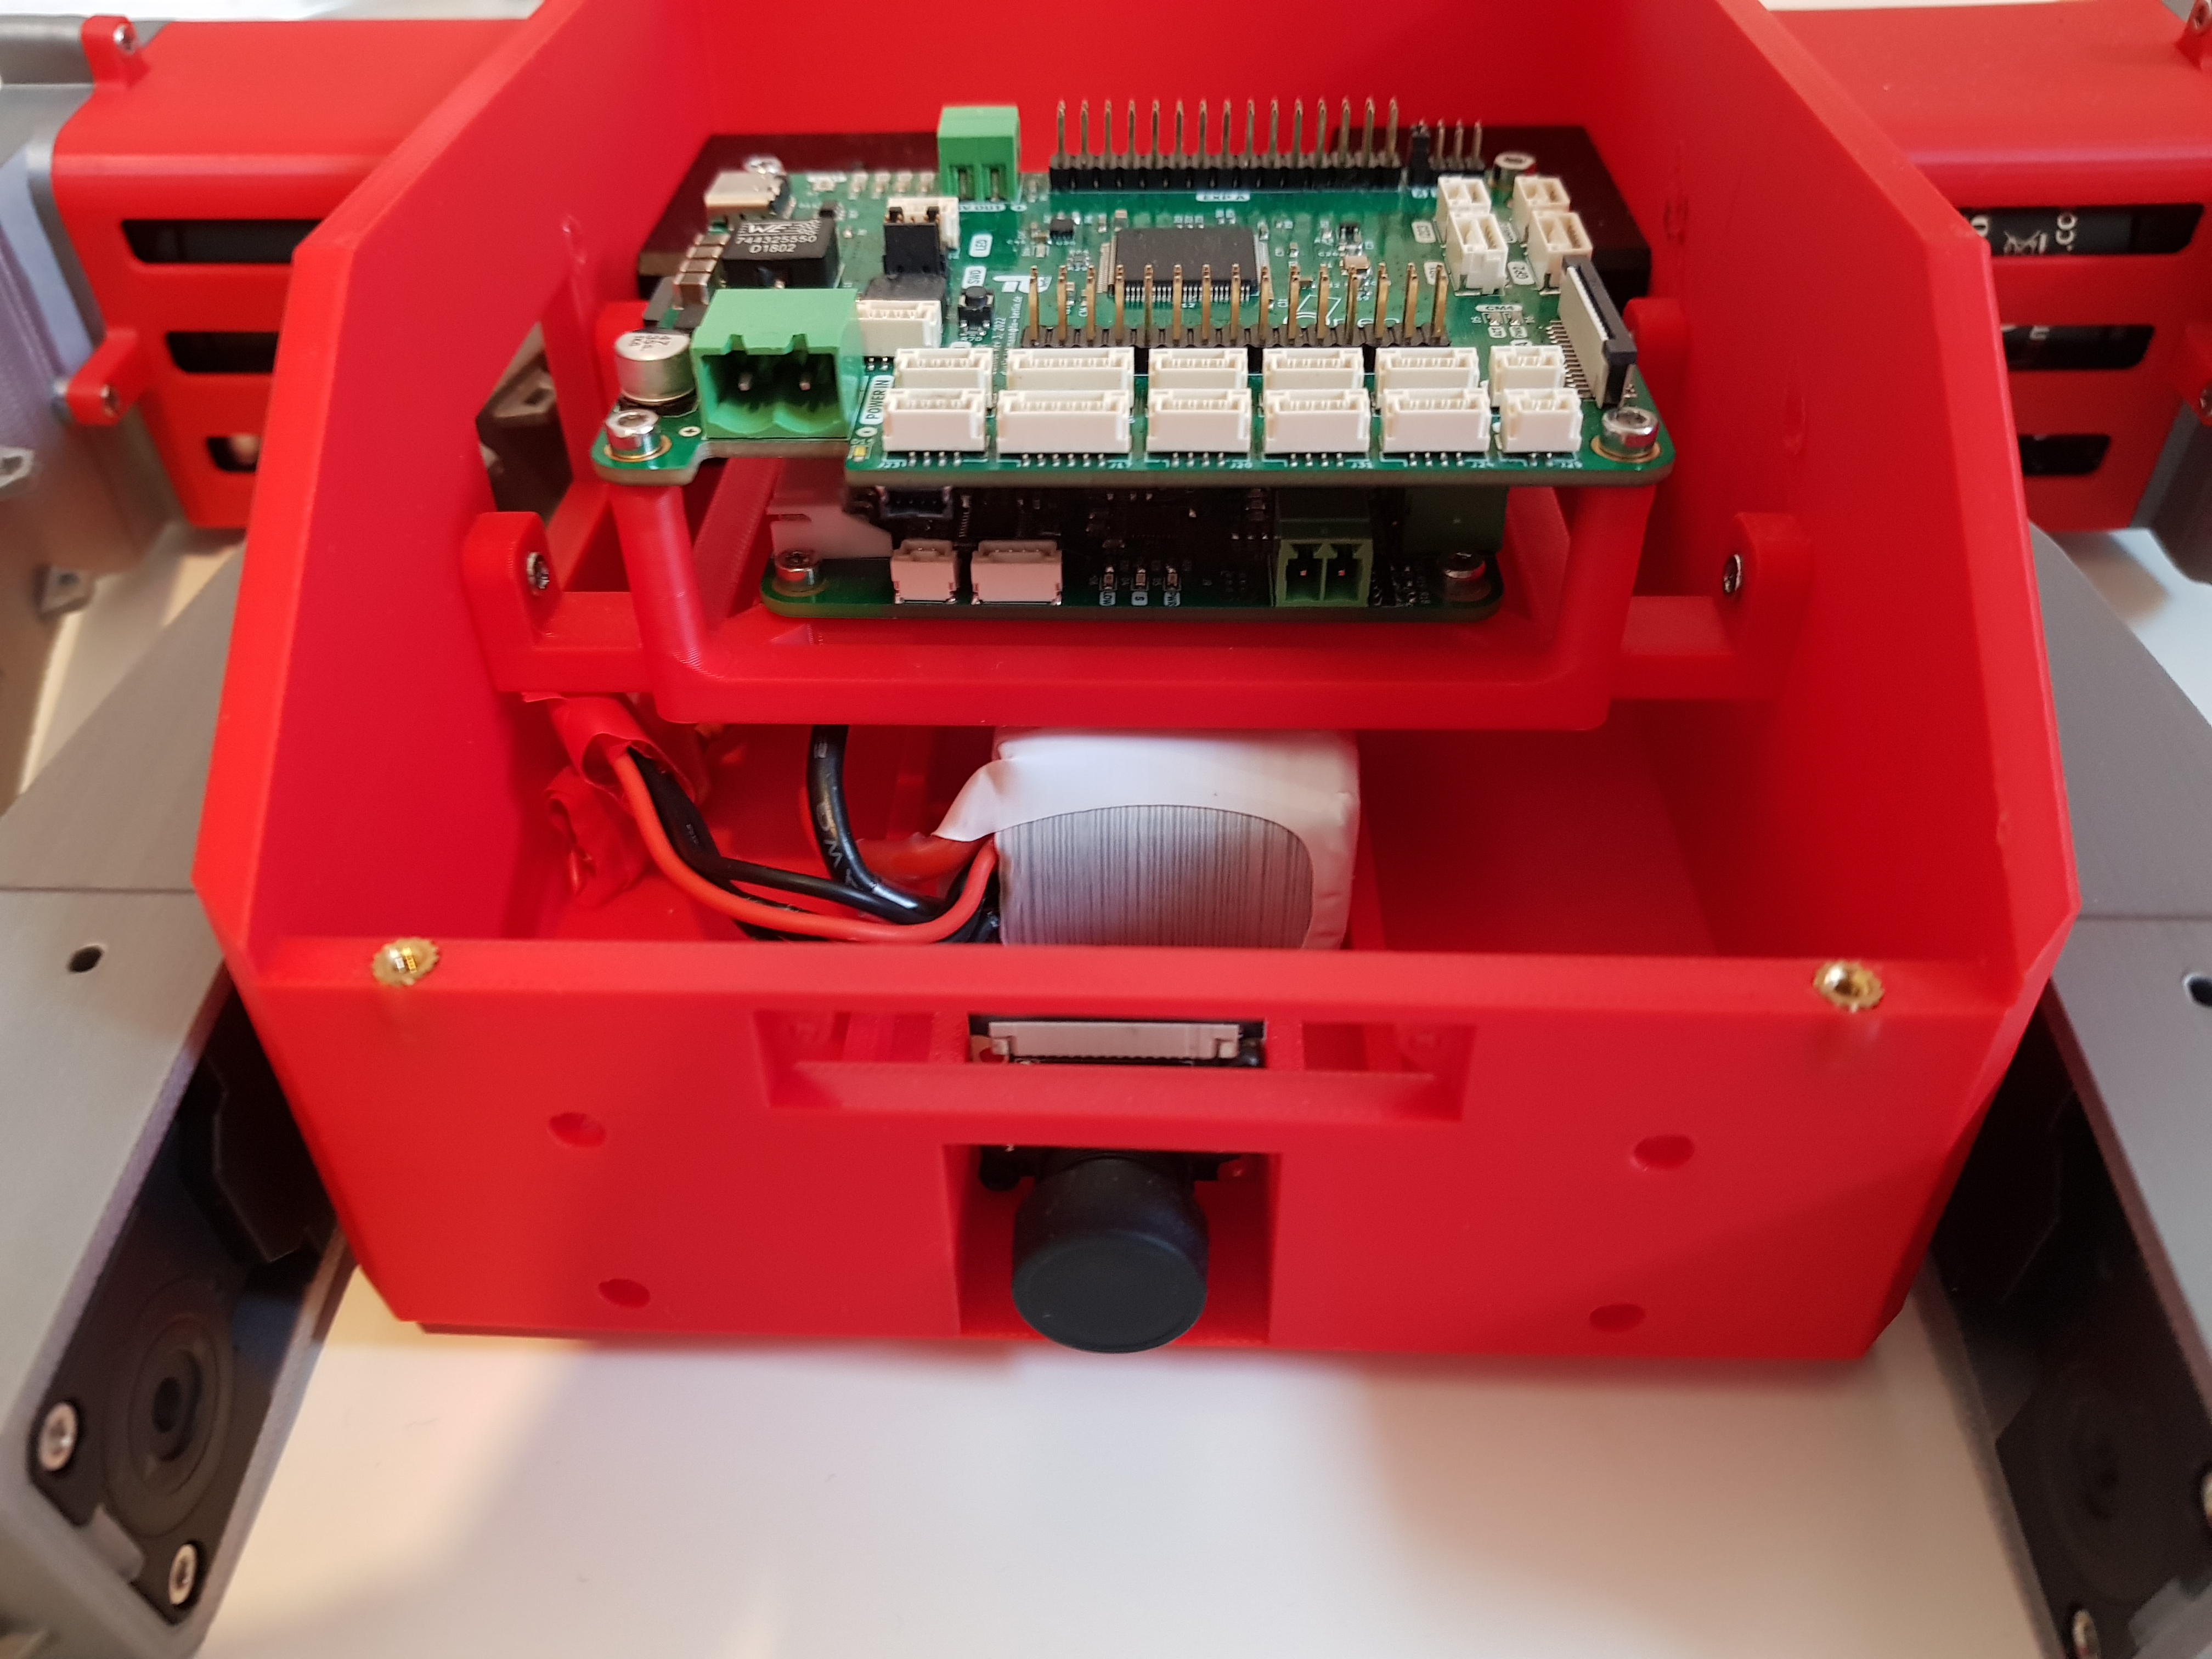
\includegraphics[width=0.5\linewidth]{electronics_mounted_on_board_mounting_rack}
	\caption{Electronics mounted on board mounting rack}
	\label{fig:electronicsmountedonboardmountingrack}
\end{figure}
%the process of connecting the wires to the board.
%measurments of the wires used
\begin{itemize}
\item Discussion on how mechanical components interface with electronic systems.
\item Challenges faced in integration and strategies employed to overcome them.
\end{itemize}

\section{Troubleshooting and Problem Solving}
%the knee motor was touching the screw so we had to shorten the screw
%the knee motor didn't fit in the link two solutions were considered either to file the link or to reprint with new dimentions.
\begin{itemize}
\item Discussion of any unexpected challenges or issues faced during assembly.
\item How these issues were diagnosed and resolved.
\end{itemize}
\section{Safety Considerations}
%cable lengthens
% cables touching the motors
\begin{itemize}
	\item Safety measures taken during the assembly process.
	\item Design considerations for ensuring the operational safety of the robot.
\end{itemize}
\begin{itemize}
	\item \textbf{Discrete Numerical Simulation:} Elaboration on the process of discrete numerical simulation, including the discrete double integration method to arrive at the state vector.
\end{itemize}

\begin{notebox}
	the bolts used the problem to shorten them so that it wouldn't touch the motor 
\end{notebox}


\chapter{Firmware and Testing}

\graphicspath{{./Figures/Firmware and Testing/}}
In this chapter, the firmware development process is detailed, including the programming languages and tools used, the integration with hardware, and the testing framework and methodology.
The test cases and scenarios are presented, along with the results of the testing procedures.
Finally, the process of debugging and troubleshooting encountered problems is discussed.

%\begin{itemize}
%	\item Overview of the chapter's content and its significance in the context of the overall project.
%	\item Briefly state the objectives of firmware development and testing procedures.
%\end{itemize}
\newpage

\section{Firmware Development}
%\begin{itemize}
%	\item Discuss the development environment and tools used for firmware programming.
%	\item Detail the architecture and design of the firmware, including flowcharts or state  diagrams if applicable.
%	\item Explain the implementation of key functionalities such as control algorithms, sensor integration, and actuator management.
%\end{itemize}
\section{Programming Languages and Tools}
%\begin{itemize}
%	\item List and describe the programming languages used for firmware development.
%	\item Mention any specific software tools, libraries, or frameworks employed.
%\end{itemize}
Mainly, the firmware is written in C language, with some parts written in C++.The STm32CubeIDE is used as the IDE for the firmware development.
Using the Cube IDE, the STM32CubeMX is used to generate the initialization code for the microcontroller.
%figure for the Pinout & Configuration
\begin {figure}[h]
\centering
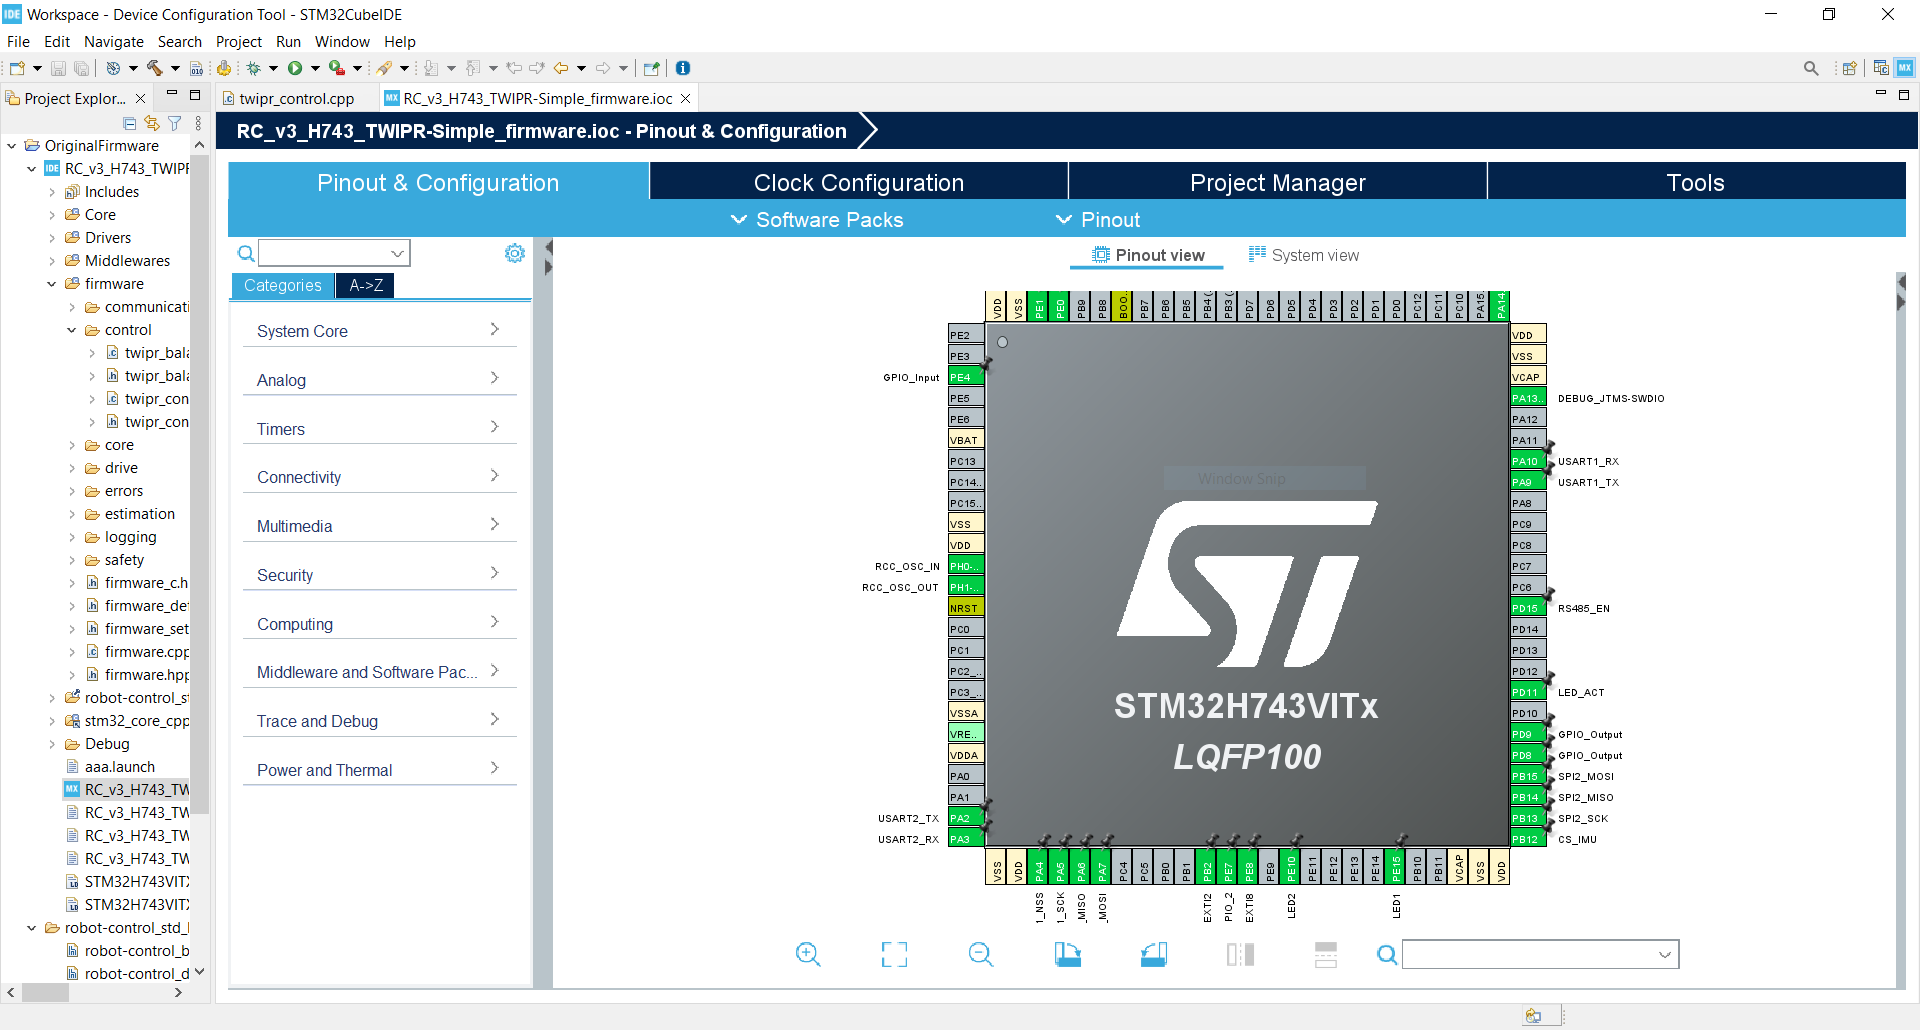
\includegraphics[width=.8\textwidth]{Pinout & Configuration}
\caption{Pinout \& Configuration}
\label{fig:Pinout}
\end {figure}

The stm32CubeIDE can configure the microcontroller peripherals, such as the GPIOs, timers, and UART. After configuring the microcontroller, the STM32CubeIDE generates the initialization code for the user.
%figure for the clock confugration
\begin {figure}[h]
\centering
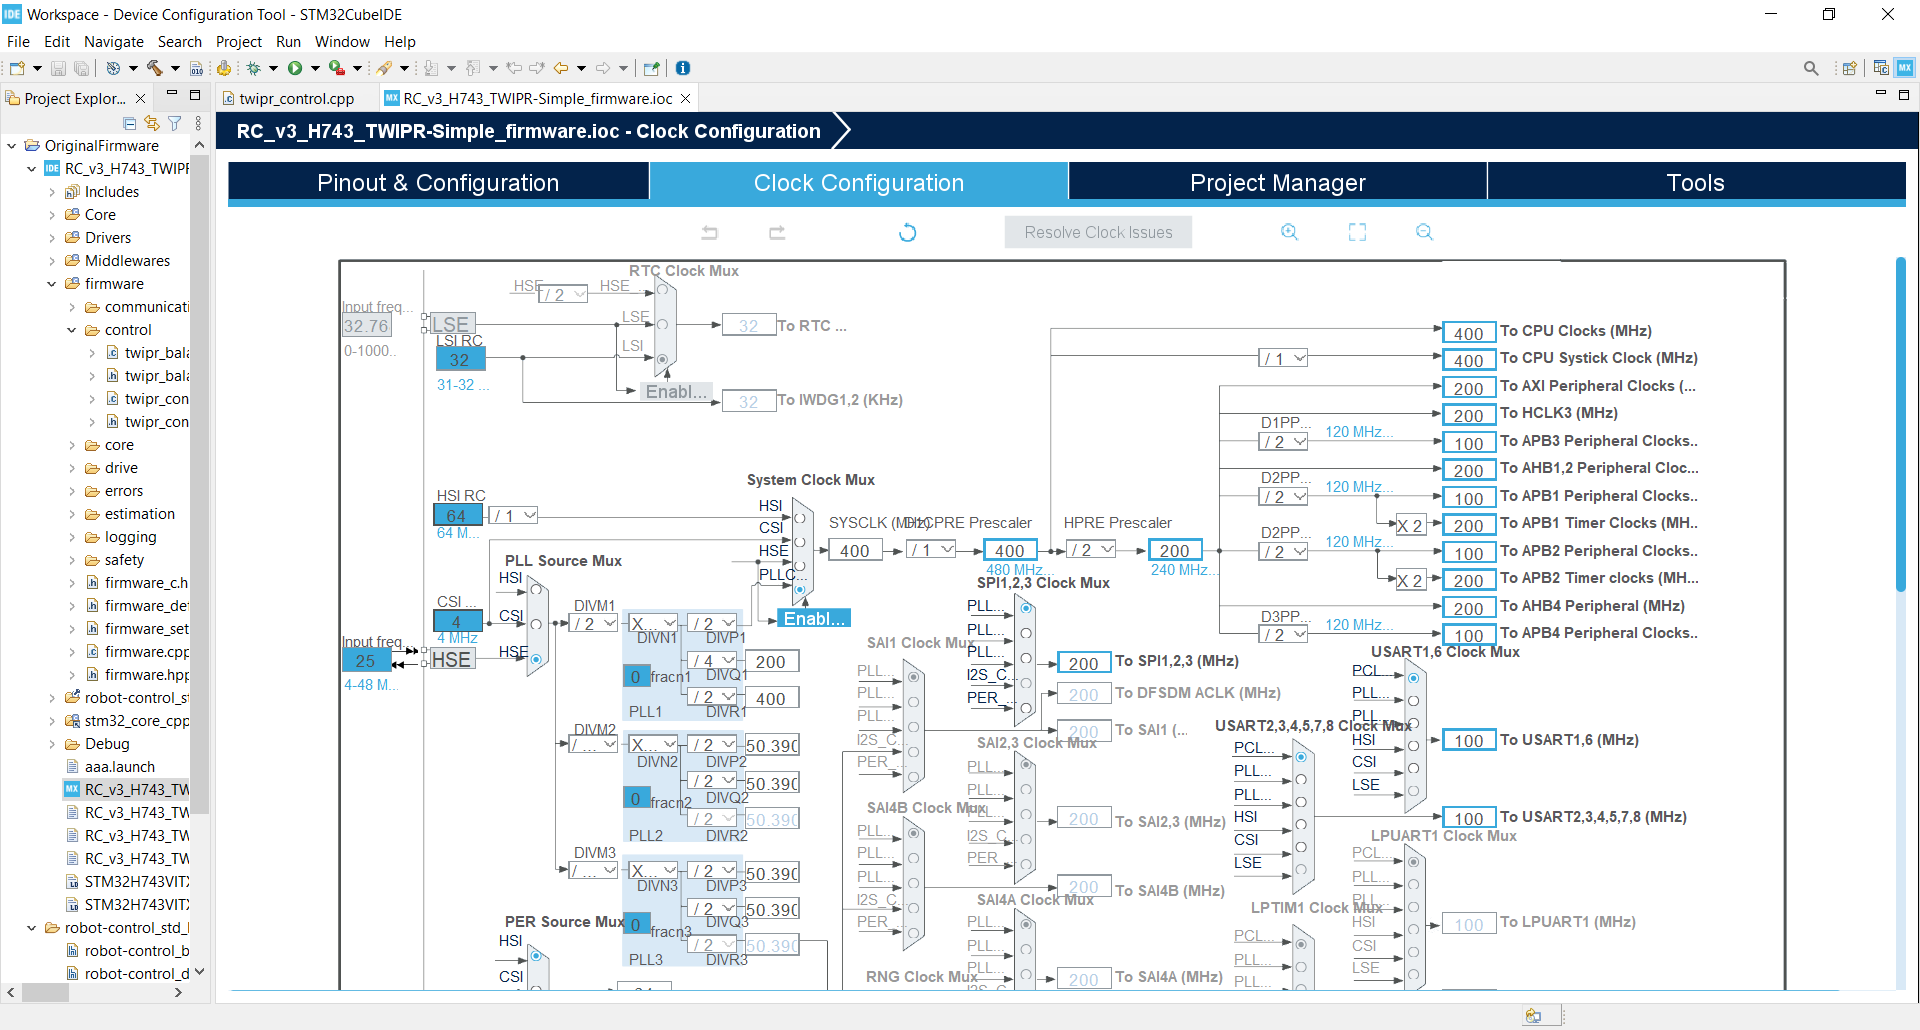
\includegraphics[width=.8\textwidth]{Clock Configuration}
\caption{Clock Configuration}
\label{fig:clock}
\end {figure}

The STM32CubeIDE allows clock configuration for the microcontroller.


The STM32Cube also generates the Makefile for the project, which is used to compile the firmware.
The STM32CubeIDE is used to compile the firmware and upload it to the microcontroller.
The STM32CubeIDE is based on the Eclipse IDE, which is an open-source IDE.


Python is also used to pass the control parameters to the microcontroller using the UART. The wireless SSH connection allows the user to change the control parameters without the need to connect the microcontroller to the computer as long as the raspberry pi and the pc are connected to the same network.

\section{Integration with Hardware}
The robot hub Board is used to connect the microcontroller to the sensors and actuators. It also provides the power supply for the microcontroller as well as acting as a carrier board for raspberry pi.
The robot hub board allows using the full potential of the microcontroller by providing the necessary connections.
%\begin{itemize}
%	\item Discuss how the firmware interacts with and controls the hardware components.
%	\item Explain any challenges encountered in integration and how they were resolved.
%\end{itemize}
\section{Testing Framework and Methodology}
%\begin{itemize}
%	\item Outline the testing framework used to validate the firmware.
%	\item Describe the methodology for functional testing, including unit tests, integration tests, and system-level tests.
%\end{itemize}
\section{Test Cases and Scenarios}
%\begin{itemize}
%	\item Present the results of the testing procedures.
%	\item Analyze these results, highlighting successful areas and identifying any issues or bugs discovered.
%\end{itemize}
\newpage
\section{Debugging and Troubleshooting}
%\begin{itemize}
%	\item Discuss the process of debugging and troubleshooting encountered problems.
%	\item Explain how issues were diagnosed and resolved.
%\end{itemize}
%figure for Jlink
\begin {figure}[h]
\centering
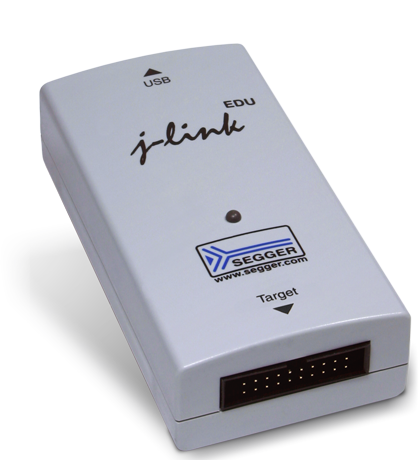
\includegraphics[width=0.5\textwidth]{jlink}
\caption{Jlink Debugger}
\label{fig:Jlink}
\end {figure}


Jlink is used to upload the firmware to the microcontroller.
As well as debugging the firmware.
The Jlink is a hardware debugger that connects to the microcontroller using the SWD interface.
The Jlink allows debugging breakpoints and stepping through the code.



\chapter{Conclusion and Future Work}

\graphicspath{{./Figures/Modeling}}

\section{Conclusion}
%This section should summarize the main findings of the research and demonstrate how they address the research questions or gaps in knowledge identified in the introduction.
%Summary of Key Findings
In this research, we developed a multi-legged robotic system that can perform complex movements and interact with its environment.
A new design was created from scratch to meet the requirements of the project.
Throughout the design process, the mechanical, electrical, and software requirements of the robot were taken into account.
Modeling of the new design was done to determine the robot's dynamics.
The modeling includes the new robot's kinematics and dynamics integrating the changing location of the center of mass of the robot as well as the changing  moments of inertia of the robot.
the model was used to simulate the robot's motion and control.
the simulation was used to test different control strategies and simulate the dynamic behavior of the robot.

The new design serves as a platform for future research and development.
The new design is modular and can be easily modified to accommodate different requirements.
The new design is also easily repairable.
The simulation results prove the validity of the model and the effectiveness of the control strategies.
The simulation results also show that the robot can change its configuration and maintain its balance.

Different challenges were faced during the development of the robot.
The main challenges were the mechanical design and the control of the new model in different configurations.
There are still some challenges and limitations that need to be addressed in future work.

\section{Future Work}
%This section should outline any future work that could be done to extend the research.
In future work, Refinement of the design for efficiency, stability.
The next generation design can be more compact and lighter.
Modeling as well can still be improved to include more details and more accurate parameters.
Additionally, implementation of more advanced control strategies can be done.
Different advanced capabilities can be integrated into the robot such as autonomous navigation, machine-learning-based control systems, or enhanced interaction with the environment.
The new robot design can take advantage of the two independent legs to perform more complex movements such as bending one knee more than the other in fast and tight turns.
Collaborative and swarm robotics can be explored, where multiple robots can work together to achieve a common goal.
%\chapter{Safety}

\graphicspath{{./Figures/Modeling}}

\begin{itemize}
	\item hardware.
	\begin{itemize}
		\item motors 
			\begin{itemize}
				\item Hip motor is enclosed in the body. 
				\item the knee motors are enclosed in cover.
				\item the wheels motors have a 
			\end{itemize}
		\item wiring 
		\begin{itemize}
			\item where the wires are neatly fastened in a predetermined route so that it wouldn't be caught in the robot movement which would cause damage to the robot and also to protect them from damage.  
			\item the correct type were used to avoid overheating upon the draw of current from the divers.
			\item Rs-485 connection between motors where used to avoid additional cables.
		\end{itemize}
	
		\item proximity sensor
		\begin{itemize}
			\item  placed in the front and back side of the robot would help to detect crashing in trivial positions such as running into a wall and that could be easily prevented by proximity sensor monitoring the distance between the robot the and the obsticals in it direction. 
		\end{itemize}
			
		\item body safety additional parts in case of impact to protect the internal components. 
	\end{itemize}
	\item software.
	
\end{itemize}


Questions to answer in each section 


\begin{enumerate}
	\item what is going to be in here?
	\item how long or how elaborate?
	\item what is the purpose (the take home message)? 
\end{enumerate}





Table of content Draft
\begin{enumerate}
	\item Introduction
	\begin{enumerate}
		\item Background and Motivation
		\begin{enumerate}
			\item Discuss the evolution and significance of robotics in various industries.
			\item Emphasize the need for advancements in robotic stability and mobility.
		\end{enumerate}
		
		\item Problem Statement
		\begin{enumerate}
			\item Define the specific challenges in designing a legged self-balancing robot.
		\end{enumerate}
		\item Objectives(Outline the primary goals of the thesis)
	\end{enumerate}
	\item Literature Review
	\begin{enumerate}
		\item Overview of Robotics
		\item Previous Work in Self-Balancing Robots
		\item Control Strategies 
		\begin{enumerate}
			\item what is going to be in here? a comparison of the control strategies used.
			\item how long or how elaborate? not too detailed but with more explanation of the control theory used in the project
			\item what is the purpose (the take home message)? pros and cons of the different and why would we prefer one of them over the other depending on the applications
		\end{enumerate}
	\end{enumerate}
	\item Design and Development of the Robot
	\begin{enumerate}
		\item Mechanical Design
		\begin{enumerate}
			\item Initial calculations 
			\begin{enumerate}
				\item what is going to be in here? -> torque initial calculations
				\item how long or how elaborate? -> two or three scenarios
				\item what is the purpose (the take home message)? for choosing the correct motors 
			\end{enumerate}
			\item design 
			\begin{enumerate}
				\item what is going to be in here?-> CAD design and the explanations of the challenges 
				\item how long or how elaborate? detailed explanations of the reason behind the design decision
				\item what is the purpose (the take home message)? assembling the robot with fitting parts to match the new model requirements  
			\end{enumerate}
			\item Modeling 
			\begin{enumerate}
				\item what is going to be in here?-> the figures for the new model and the new COG and MOI calculations and the equations of motion.  
				\item how long or how elaborate? 4 to 5 pages explaining the equations in details 
				\item what is the purpose (the take home message)? showing the calculations for the new model and it would influence the equations of motion.
			\end{enumerate}
		\end{enumerate}
		\item Electrical Design
		\begin{enumerate}
			\item what is going to be in here? Component diagram showing the choice of all the components and there intended use and why we chose each of these components 
			\item how long or how elaborate? detailed explanation of the  requirement boards for operating the robot, the choice of components based calculations for the motors.
			\item what is the purpose (the take home message)? show how the Electrical design is configured in the optimal way to operate the robot 
		\end{enumerate}
		\item Software and Control
		\begin{enumerate}
			\item Control Algorithm 
			\begin{enumerate}
				\item what is going to be in here?->flowchart of the Control Algorithm
				\item how long or how elaborate?-> detailed explanation of the used control theory 
				\item what is the purpose (the take home message)? -> how the control is implemented 
			\end{enumerate}
			\item Firmware
		\end{enumerate}
		\item Safety 
		\begin{enumerate}
			\item what is going to be in here? different design changes for safety measures(motors covers, wire routing, body bumper, distance sensor , algorithm safety, electrical safety )
			\item how long or how elaborate? 1 or two pages max that include the 
			\item what is the purpose (the take home message)? the safety measures taken to minimize crashes, failure
		\end{enumerate}
	\end{enumerate}
	\item Experimental Setup and Methodology
	\begin{enumerate}
		\item Simulation Environment
		\item Physical Prototype Testing
		\item Data Collection and Analysis
	\end{enumerate}
	\item Results and Discussion
	\begin{enumerate}
		\item Simulation Results
		\item Real-world Performance
		\item Comparison and Analysis
	\end{enumerate}
	\item Conclusion and Future Work
	\begin{enumerate}
		\item Summary of Findings
		\item Contributions
		\item Recommendations for Future Research
	\end{enumerate}
\end{enumerate}


\begin{todobox}
	content..
\end{todobox}
%\chapter{Random(Erase)}

\graphicspath{{./Figures/Design}}

This comprehensive chapter unfolds the intricate details of the new design of our two-wheeled self-balancing robot, an advanced piece of engineering that incorporates additional degrees of freedom to enhance its movement capabilities. Through an exploration of the various motions the robot can perform, we delve into the intricate design considerations of each component, ensuring that they align with the overall functional and aesthetic vision. 


\begin{figure}[h]
	\centering
	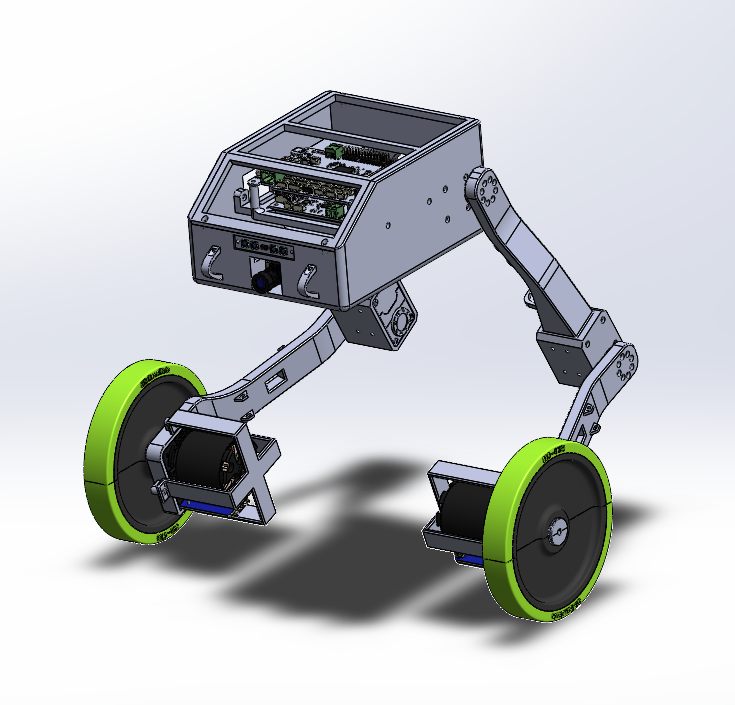
\includegraphics[width=1\textwidth]{/Capture}
	\caption[Moment of inertia Schematic representation]{Schematic representation detailing the requisite angles and lengths for calculating the moment of inertia.}
	\label{fig:Schematic representation detailing the requisite angles and lengths for calculating the moment of inertia.}
\end{figure}
\newpage
\begin{itemize}
	\item The Robot new design.
	\item The added degrees of freedom.
	\item Different motions that can be performed.
	\item Discussing each component of the robot and things taken into account while designing it.
	\begin{itemize}
		\item Body
		\begin{itemize}
		\item overall design inspiration
		\item For the body: the consideration for including all the necessary components in a compact form is to optimize the use of space and at the same time distribute the weight equally.
		\item The body includes the hip motors, the battery, camera, sensor, a rack that includes the motors drivers board, the micro-controller board attached to the Raspberry Pi.
		\item fastening features that were specifically designed in order to easily mount the battery, organize the cable between the boards and the rest of the robot parts.
		\item Features for modular design and easy printing.
		\end{itemize}
			\item Thigh
		\begin{itemize}
			\item curvature of that joint to give room for the motors 
			\item cable management 
			\item motor cover to insure its fixation. 
		\end{itemize}
			\item Calf
		\begin{itemize}
			\item curvature of that joint and the thigh joint combined make enough room for the wheel motor so the it have clearance from the body. 
			\item cable management 
			\item motor mount and additional frame.
		\end{itemize}
	\end{itemize}
\end{itemize}





\newpage


\begin{figure}[h]
	\centering
	\includegraphics[width=1\textwidth]{/Component_diagram.pdf}
	\caption[Moment of inertia Schematic representation]{Schematic representation detailing the requisite angles and lengths for calculating the moment of inertia.}
	\label{fig:Schematic representation detailing the requisite angles and lengths for calculating the moment of inertia.}
\end{figure}
\begin{itemize}
	\item electronic components 
	\begin{itemize}
		\item Motors taking into count the needed torque and speed
		\item comparison between the BLDC and Geared Robotic 
		\item RS-485 communications protocol compared to others 
		\begin{itemize}
			\item for the knee and hip motors high torque and low speed is needed.(calculations the show the weights and the needed torques)
			\item for the wheel motors high speed and low torque is needed. 
		\end{itemize}
		\item Boards 
		\begin{itemize}
			\item STM high performance h7 constum board connected with rasberrypi 
			\item driver board that provide the power for 6 motors. 
		\end{itemize}
		\item modules 
		\begin{itemize}
			\item camera module.
			\item distance sensor.
		\end{itemize}
	\end{itemize}
\end{itemize}




% % % % % % % % % % % % % % % % % % % % % % % % % % % % % % % % % % % % % % % % % % % % % % %

% Conclude Body Matter
\clearpage

%
%% Back Matter - List of figures and tables, listings, index, glossaries, etc.
% Roman numerals for Back Matter - continue page numbering from Front Matter
\pagenumbering{Roman}
\addtocounter{RomanNumbers}{1}
\setcounter{page}{\value{RomanNumbers}}

% If desired, uncomment the index
\printindex

% If desired, uncomment the bibliography
\bibliography{Bibliographie/Bibliographie}

% Conclude Back Matter
\clearpage


% If applicable, Appendix
%\appendix
% Im Anhang kleine römische Zahlen, beginnend ab i
\pagenumbering{roman}

% Hier den Anhang einfügen, z. B.
% \include{Anhang/TollesKapitel} ...





\chapter{Related Works}\label{ch:app_prior_works}
\graphicspath{{./Bilder/prior_works}} 
\begin{figure}[h!]
        \centering
        \includegraphics[width=1\textwidth]
        {schoellig_et_al_connected_papers_a_dyn_sys_pers.png}
        \caption[Connected Papers for "A dynamical systems perspective"]{Connected Papers overview based on the work "A dynamical systems perspective" showing how tightly interconnected papers from Schoellig et al. are on this topic. The authors Schoellig, Pereida, Zhou, Rimalwala, Helwa and Sorocky are seemingly one research group, making up the majority of the more recent papers in that field.}\label{fig:connected_papers}
\end{figure}



\chapter{Method}
% ____________________________________________________________________
% ======================== Spring Damper System =====================
\section{Input Types}\label{sec:app_meth1}
\graphicspath{{./Bilder/transfer_function_estimation}} 
% ====================================================================


% ===============================================================
% =================  INPUT TYPE: STEP Long ===============
\begin{example}[: Step input (long)]\label{ex:step_input_long}
	Consider the same example systems and method as presented in \exref{ex:single_sine_input_01hz}.
    Both systems are excited using a step signal. The final step value is held for 
    \begin{equation}
        t_{\mathrm{step\,hold}} = 100\,s.
    \end{equation} 
     The estimated input transfer is
     \begin{equation}
        \hat{T}^{(1 \rightarrow 2)}(z) = \frac{0.347\,z - 0.345}{z - 0.999} 
     \end{equation}
     \begin{notebox}
     Note that the longer hold duration results in a smaller error gain for slow frequencies but increases the maximum error gain $\|H^{(1 \rightarrow 2)}\|_{\infty}$.
     \end{notebox}

\begin{minipage}{1\textwidth}
\begingroup
	\centering
	\vspace{1em}
	\captionsetup{format=plain, type=figure, labelfont={color=example_font_color, bf}, font={color=example_font_color}}
    \begin{subfigure}[t]{0.495\textwidth}
        \centering
        \includegraphics[width=\textwidth]{/input_types/step 100 time.pdf}
        \caption{System response to a step training input with and without the estimated input-transfer}
        \label{subfig:tf_est_input_step2_time}
    \end{subfigure}
    \hfill    
    \begin{subfigure}[t]{0.495\textwidth}
        \centering
        \includegraphics[width=\textwidth]{/input_types/step 100 bode.pdf}
        \caption{Bode diagram of the error dynamics with and without the estimated input-transfer}
        \label{subfig:tf_est_input_step2_bode}
    \end{subfigure}
    \caption[Training Inputs for Transfer Map Estimation (Step II)]{Estimated input-transfer from a unit step training input which was held for $t_{\mathrm{step\,hold}} = 100\unit{s}$}
    \label{subfig:tf_est_input_step2}
\endgroup
\end{minipage}
\end{example}



%%%%%%%%%%%%%%%%%%%%%%%%%%%%%%%%%%%%%%%%%%%%%%%%%%%%%%%%%%%%%%%%%%%%%%%%%%%%%%
% ============================================================================
% =================  INPUT TRANSFER ORDER: INPUT SET  ===================
\section{Input Transfer Order}\label{subsecapp:input_transfe_order}
% -------------------------------------------------------------------
\graphicspath{{./Bilder/appendix/tf_order}} 
\begin{commentnotes}
\textbf{Main Idea}
\vspace{-0.5em}
\begin{itemize}[noitemsep, topsep=0pt]
	\item The order of the \gls*{transfer_map} impacts the transfer performance. We would expect, that a transfer of lower order can still achieve good results for certain frequencies. Training data from random input trajectories is used to estimate \glspl*{input_map} of different orders between two known second-order systems. The transfer error dynamics as well as the training and test errors are evaluated for all system orders. Additionally, the training data is deteriorated by output noise and the estimation is repeated.
\end{itemize}

\textbf{Conclusions}
\vspace{-0.5em}
\begin{itemize}[noitemsep, topsep=0pt]
	\item A constant gain hardly decreases the direct transfer error. A system order of at least 2 is recommended.
	\item The best transfer is achieved for the ideal system order of $K=3$
	\item Without noise, a higher system order has no real impact.
	\item With noise, a too high system order results more often in negative transfer. 
	\item With noise, higher frequencies, not part of the training (and test) input, resulted in high transfer errors. (especially for higher transfer errors)
\end{itemize}
\end{commentnotes}
% -------------------------------------------------------------------


This section explores how the model order choice impacts the transfer error dynamics for two second-order example systems. The setup is given in detail in \exref{exapp:input_transfer_order}. The main results are described in the following. 

Given two second-order \acrshort{lti} \acrshort{siso} systems with a relative order of one, the order of the ideal transfer map from \eqref{eq:ideal_sys_order} is $K=3$.
Since both systems have the same system order and relative degree, they are structurally similar. The relative degree of the ideal transfer is $m=0$.

A trivial transfer choice is a static map with only a single scalar parameter tuned to transfer trajectories between two systems. This is equivalent to a transfer function of order $K=0$. As seen in \secref{subsec:static_map}, a static map cannot account for frequency-dependent differences in the phase and gain of the systems.
%The resulting dynamics of the transfer error are mainly impacted by the choice of the training input.  
While this transfer is easily implemented, the benefits are limited to specific inputs, and the decrease in the transfer error compared to the direct transfer is only marginal. The transfer error dynamics for $K=0$ are shown for the two example systems in \figref{subfigapp:tf_order_a}.

Increasing the order of the estimated \gls*{input_map} to $K=1$ improves the transfer performers. However, a transfer function of order one lacks the ability to model oscillating behaviour. This may be the reason why the transfer error is still very high over a large range of inputs. This is seen in \figref{subfigapp:tf_order_c}.

When the order of the estimated system is increased to $K=2$, the error dynamics show a sudden improvement over the previous order of $K=1$. This can be seen especially in the substantial decrease of the maximum error gain $h_{\infty}$ seen in \figref{subfigapp:tf_order_e}. This may be to its ability to model oscillating behaviour. 

The ideal model order of $K=3$ results in the best overall transfer performance. Under perfect conditions\footnote{no disturbances / noise affect the outputs of the training input}, the estimated transfer function is so similar to the ideal \gls*{input_map} that only an insignificant transfer error remained, even for frequencies not contained in the training data (\figref{subfigapp:tf_order_g}).

Increasing the model order further ($K>3$) does not affect the transfer error under ideal conditions. However, if output noise deteriorates the training data even slightly, outliers with very poor transfer performance become more frequent with a higher model order of the estimated \gls*{transfer_map}. 

The effect of output noise is most noteworthy in higher frequencies, which are absent in the deterministic training input. 
This may result in a large difference between training and test errors. Increasing the model order leads to a greater difference in transfer errors between the perfect training data and data corrupted with output noise. This indicates that lower-order systems are more resilient to imperfect training data than higher-order systems. 
\figref{figapp:input_transfer_order} illustrates the transfer error dynamics in the absence of output noise on the left side and in the presence of noise on the right side.


\begin{notebox}[Random trajectories]\label{noteapp:sample_random_input}
	\textbf{How random trajectories of length $N$ and magnitude $\sigma_{\vec{u}}$ are generated in this work}~\\
	\vspace{-1em}
	\begin{enumerate}[noitemsep, topsep=0pt]
		\item A sequence of random samples is drawn from a uniform distribution.
		\item The sequence is filtered using the MATLAB method \texttt{filtfilt()} with a 6th-order Butterworth filter with a cutoff frequency of $f_{\mathrm{cutoff}}$.
		\item A sequence $\vec{u}$ containing $N$ samples is selected from the filtered sequence so that the initial value $u_0$ is close to zero. 
		\item The \textit{peak-to-rms factor} (\textit{crest factor}) of $\vec{u}$ is evaluated using the MATALB method \texttt{peak2rms}, so that $\texttt{peak2rms}(\vec{u}) \leq 3$ is given. If not, a new sequence is drawn. 
		\item The sequence $\vec{u}$ is rescaled so that its standard deviation $\mathrm{std}(\vec{u})$ matches 
		$2\sigma_{\vec{u}}$. (I.e. for $\sigma_{\vec{u}}=1$, the standard deviation of the sequence $\mathrm{std}(\vec{u})=2$, which means that most of the signal lies between $-1$ and $1$)
	\end{enumerate}	
	See the file \filenamecode{fun\_sample\_random\_input.m}.	
\end{notebox}

% -------------------------------------------------------------------
\begin{commentnotes}
\begin{table}
        \renewcommand{\arraystretch}{1.3}
        \begin{tabularx}{1\textwidth}{@{}ccccccc@{}}
            \toprule
            \textbf{Order} & \phantom{a} & \multicolumn{2}{c}{\textbf{Training Error}} & \phantom{abc} & \multicolumn{2}{c}{\textbf{Test Error}} \\ \cmidrule{3-4} \cmidrule{6-7}
            $K$ && $\sigma = 0$ & $\sigma = 0.05$ && $\sigma = 0$ & $\sigma = 0.05$ \\ \midrule
            $0$ && $9.6 \cdot 10^{-1}$ & $9.6 \cdot 10^{-1}$ && $9.8 \cdot 10^{-1}$ & $9.8 \cdot 10^{-1}$ \\
            $1$ && $8.2 \cdot 10^{-1}$ & $8.2 \cdot 10^{-1}$ && $8.4 \cdot 10^{-1}$ & $8.5 \cdot 10^{-1}$ \\
            $2$ && $5.6 \cdot 10^{-2}$ & $1.7 \cdot 10^{-1}$ && $6.0 \cdot 10^{-2}$ & $1.8 \cdot 10^{-1}$\\
            $3$ && $4 \cdot 10^{-15}$ & $0.9 \cdot 10^{-1}$ && $4 \cdot 10^{-15}$ & $1.0 \cdot 10^{-1}$\\
            $4$ && $4 \cdot 10^{-15}$ & $5.6 \cdot 10^{-2}$ && $4 \cdot 10^{-15}$ & $6.2 \cdot 10^{-2}$\\
            $5$ && $3.5 \cdot 10^{-11}$ & $9.4 \cdot 10^{-1}$ && $4.1 \cdot 10^{-11}$ & $9.5 \cdot 10^{-1}$\\
            $6$ && $4.2 \cdot 10^{-5}$ & $8.1 \cdot 10^{-1}$ && $5.3 \cdot 10^{-5}$ & $8.0 \cdot 10^{-1}$\\
%            $•$ & $• \cdot 10^{-1}$ & $• \cdot 10^{-1}$\\
%\multirow{2}{*}{\textbf{Order} $K$}
            \bottomrule
        \end{tabularx}
        \caption[Test and Training Errors of Input Transfer Maps for various System Orders]{Average training and test error for different system orders $K$ of the estimated \gls*{input_map} dynamics without output noise $\sigma = 0$ and with output noise $\sigma = 0.05$ in the training data}
        \label{tab:input_transfer_transfer_order}
\end{table} 
\end{commentnotes} 
% -------------------------------------------------------------------


% ============================================================================
\begin{example}[System order of the estimated input transfer map]\label{exapp:input_transfer_order}
%\paragraph{Input Set}\label{frame:input transfer order: input set}~\\
Consider the following two second-order minimum phase \glsxtrshort{lti} \glsxtrshort{siso} systems
\begin{equation}
    F^{(1)}(s) = \frac{2s+1}{0.9s^2+1.2s+0.5} \quad
    F^{(2)}(s) = \frac{0.5s+1}{1s^2+0.5s+1}\,. \label{eqapp:example_order_change}
\end{equation}
\figref{figapp:input_tf_order_training_data_bode} shows the bode plot of the two systems and their corresponding error dynamics.

\begingroup
	\centering
	\vspace{1em}
	\captionsetup{format=plain, type=figure, labelfont={color=example_font_color, bf}, font={color=example_font_color}}
        \includegraphics[width=0.5\textwidth]{/system_order/input transfer order systems bode.pdf}
        \caption[System Order of Transfer Maps Example (Bode Plot of the Error Dynamics)]{Bode plot of systems $F^{(1)}(s)$ and $F^{(1)}(s)$ and their error dynamics $H^{(1,2)}(s)$}
		\label{figapp:input_tf_order_training_data_bode}
\endgroup

Consider multiple input trajectories 
\begin{equation}
    \vec{u}_l \in (\mathcal{U}^{(i,j)})^N \quad
    \text{for} \quad l \in [1,\ldots,20] 
% &&\text{, } |\mathcal{U}| = 20
\end{equation} 
Each input $\vec{u}_l$ is a random input trajectory of length $t=50\unit{s}$ and magnitude one which is drawn according to \noteref{note:sample_random_input}. A sampling rate of $f_s = 100\unit{Hz}$ was chosen. \figref{subfigapp:input_tf_order_training_data_in} shows some of the randomly generated input trajectories, with one trajectory highlighted. The corresponding deterministic ($\sigma = 0$) outputs of the systems $F^{(1)}$ and $F^{(2)}$ to the inputs are shown in \figref{subfigapp:input_tf_order_training_data_out}.

In a second case, a noise sequence $\vec{w}$ is added to the deterministic output trajectories, with  
\begin{equation}
    w \sim  \mathcal{N}(0,\sigma^2) \quad
    \forall w  \in \vec{w} \qquad \text{and}
    \qquad \sigma = 0.05\,.
\end{equation} 
The resulting output trajectories, including the additional noise, are depicted in \figref{subfigapp:input_tf_order_training_data_out2}.

\begin{minipage}{1\textwidth}
\begingroup
	\centering
	\vspace{1em}
	\captionsetup{format=plain, type=figure, labelfont={color=example_font_color, bf}, font={color=example_font_color}}
    \begin{subfigure}[t]{0.515\textwidth}
        \centering\captionsetup{width=.9\linewidth}
        \includegraphics[width=\textwidth]{/system_order/input transfer order input set.pdf}
        \caption{Some training inputs with one input highlighted}
        \label{subfigapp:input_tf_order_training_data_in}
    \end{subfigure}
    \hfill
    \begin{subfigure}[t]{0.495\textwidth}
        \centering\captionsetup{width=.9\linewidth}
        \includegraphics[width=\textwidth]{/system_order_noise/input transfer order output set.pdf}
        \caption{Corresponding deterministic output trajectories to the training inputs}
        \label{subfigapp:input_tf_order_training_data_out}
    \end{subfigure}
    \hfill
    \begin{subfigure}[t]{0.495\textwidth}
        \centering\captionsetup{width=.9\linewidth}
        \includegraphics[width=\textwidth]{/system_order_noise/input transfer order output set noise 0.050.pdf}
        \caption{Corresponding output trajectories to the training inputs with artificial noise}
        \label{subfigapp:input_tf_order_training_data_out2}
    \end{subfigure}
    \caption[System Order of Transfer Maps Example (Training Data)]{Training data for \gls*{input_map} estimation of different system orders}
    \label{figapp:input_tf_order_training_data}
\endgroup
\end{minipage}
 

% ============================================================================
% =================  INPUT TRANSFER ORDER: EXAMPLE SYSTEMS  ==================

For every input $\vec{u}_l$ an \gls*{input_map} $\hat{T}^{(1 \rightarrow 2)}_l(s)$ with $l = 1,\ldots, 20$ of order $K$ in the form of \eqref{eq:estimated_tf} is estimated using the corresponding outputs $\left(\vec{y}^{(1)}, \vec{y}^{(2)}\right)_{\vec{u}_l}$. Each \gls*{input_map} is estimated once using the deterministic output trajectories and once under the presence of output noise.\\ 
The system orders of the estimated \glspl*{input_map} are increased from zero to six, so that
\begin{equation}
	K = 0,\ldots,6\,.
\end{equation}
Note that the ideal order of the \gls*{input_map} for the sytems in \eqref{eqapp:example_order_change} is $K=3$.\\

    For an \gls*{input_map} $\hat{T}^{(1 \rightarrow 2)}_l(s)$, the training error $e^{(1 \rightarrow 2)}_{\vec{u}, \mathrm{NRMS}}(\vec{u}_l)$ is calculated using the training input $\vec{u}_l$.\\
    The test error $e^{(1 \rightarrow 2)}_{\vec{u}, \mathrm{NRMS}}(\vec{u}_k)$ is calculated using the remaining test inputs $\vec{u}_k$ for $k = 1,\ldots,20$ and $k\neq l$.
    
    We then average the training error and test error over all estimated \glspl*{input_map} 
    $\hat{T}^{(1 \rightarrow 2)}_l(s)$. This is shown in \figref{figapp:tf_order_error}.
    
    The resulting transfer error dynamics are shown in \figref{figapp:input_transfer_order}.

\begin{minipage}{1\textwidth}
\begingroup
	\centering
	\vspace{1em}
	\captionsetup{format=plain, type=figure, labelfont={color=example_font_color, bf}, font={color=example_font_color}}
           \includegraphics[width=0.6\textwidth]{/system_order_noise/error_over_order.pdf}
           \caption[System Order of Transfer Maps Example (Test and Training Errors)]{Mean training error and mean test error over the order of the estimated biproper transfer function with ($\sigma = 0.05$) and without ($\sigma = 0$) noise in the training trajectories}
           \label{figapp:tf_order_error}
       \endgroup
\end{minipage}

    
% ===================================================================
\begingroup
	\centering	
	\captionsetup{format=plain, type=figure, labelfont={color=example_font_color, bf}, font={color=example_font_color}}
	\begin{minipage}{1\textwidth}
	\vspace{1em}     
       \begin{subfigure}{0.495\textwidth}
           \centering
           \includegraphics[width=\textwidth]{/system_order/input transfer order random input s0 n0.000 bode.pdf}
           \caption{$K = 0$ and $\sigma = 0$}
           \label{subfigapp:tf_order_a}
       \end{subfigure}
       \hfill
       \begin{subfigure}{0.495\textwidth}
           \centering
           \includegraphics[width=\textwidth]{/system_order_noise/input transfer order random input s0 n0.050 bode.pdf}
           \caption{$K = 0$ and $\sigma = 0.05$}
           \label{subfigapp:tf_order_b}
       \end{subfigure}
       \hfill 
       
       \medskip      
       \begin{subfigure}{0.495\textwidth}
           \centering
           \includegraphics[width=\textwidth]{/system_order/input transfer order random input s1 n0.000 bode.pdf}
           \caption{$K = 1$ and $\sigma = 0$}
           \label{subfigapp:tf_order_c}
       \end{subfigure}
       \hfill 
       \begin{subfigure}{0.495\textwidth}
           \centering
           \includegraphics[width=\textwidth]{/system_order_noise/input transfer order random input s1 n0.050 bode.pdf}
           \caption{$K = 1$ and $\sigma = 0.05$}
           \label{subfigapp:tf_order_d}
       \end{subfigure}
       \hfill
       
       \medskip
       \begin{subfigure}{0.495\textwidth}
           \centering
           \includegraphics[width=\textwidth]{/system_order/input transfer order random input s2 n0.000 bode.pdf}
           \caption{$K = 2$ and $\sigma = 0$}
           \label{subfigapp:tf_order_e}
       \end{subfigure}
       \hfill
       \begin{subfigure}{0.495\textwidth}
           \centering
           \includegraphics[width=\textwidth]{/system_order_noise/input transfer order random input s2 n0.050 bode.pdf}
           \caption{$K = 2$ and $\sigma = 0.05$}
           \label{subfigapp:tf_order_f}
       \end{subfigure}
       \hfill
       
       \medskip
       \begin{subfigure}{0.495\textwidth}
           \centering
           \includegraphics[width=\textwidth]{/system_order/input transfer order random input s3 n0.000 bode.pdf}
           \caption{$K = 3$ and $\sigma = 0$}
           \label{subfigapp:tf_order_g}
       \end{subfigure}
       \hfill
       \begin{subfigure}{0.495\textwidth}
           \centering
           \includegraphics[width=\textwidth]{/system_order_noise/input transfer order random input s3 n0.050 bode.pdf}
           \caption{$K = 3$ and $\sigma = 0.05$}
           \label{subfigapp:tf_order_h}
       \end{subfigure}
       \vspace{1em}
\end{minipage}
%\end{figure}
%\clearpage
%\begin{figure}
%       \ContinuedFloat
\newpage
\begin{minipage}{1\textwidth}
\vspace{1em}
       \begin{subfigure}{0.495\textwidth}
           \centering
           \includegraphics[width=\textwidth]{/system_order/input transfer order random input s4 n0.000 bode.pdf}
           \caption{$K = 4$ and $\sigma = 0$}
           \label{subfigapp:tf_order_i}
       \end{subfigure}
       \hfill 
       \begin{subfigure}{0.495\textwidth}
           \centering
           \includegraphics[width=\textwidth]{/system_order_noise/input transfer order random input s4 n0.050 bode.pdf}
           \caption{$K = 4$ and $\sigma = 0.05$}
           \label{subfigapp:tf_order_j}
       \end{subfigure}
       \hfill 
       
       \medskip                   
       \begin{subfigure}{0.495\textwidth}
           \centering
           \includegraphics[width=\textwidth]{/system_order/input transfer order random input s5 n0.000 bode.pdf}
           \caption{$K = 5$ and $\sigma = 0$}
           \label{subfigapp:tf_order_k}
       \end{subfigure}
       \hfill
       \begin{subfigure}{0.495\textwidth}
           \centering
           \includegraphics[width=\textwidth]{/system_order_noise/input transfer order random input s5 n0.050 bode.pdf}
           \caption{$K = 5$ and $\sigma = 0.05$}
           \label{subfigapp:tf_order_l}
       \end{subfigure}
       \hfill
       
       \medskip  
       \begin{subfigure}{0.495\textwidth}
           \centering
           \includegraphics[width=\textwidth]{/system_order/input transfer order random input s6 n0.000 bode.pdf}
           \caption{$K = 6$ and $\sigma = 0$}
           \label{subfigapp:tf_order_m}
       \end{subfigure} 
       \hfill
       \begin{subfigure}{0.495\textwidth}
           \centering
           \includegraphics[width=\textwidth]{/system_order_noise/input transfer order random input s6 n0.050 bode.pdf}
           \caption{$K = 6$ and $\sigma = 0.05$}
           \label{subfigapp:tf_order_n}
       \end{subfigure} 
       %%%%%              
       \caption[System Order of Transfer Maps Example (Bode Plot of the Transfer Error Dynamics)]{Bode diagram of the error dynamics with and without the estimated \gls*{input_map} $\hat{T}^{(1 \rightarrow 2)}_{l}$ for different system orders $K$ of the input transfer dynamics}
       \label{figapp:input_transfer_order}
%\end{figure} 
\end{minipage}
\endgroup
\end{example} 




% =============================== EXAMPLE 0  ================================
% ============================================================================
\graphicspath{{./Bilder/transfer_function_estimation/system_order/example4}} 
\clearpage
\begin{example}[Example 1: System order - constant gain]\label{ex:input_transfer_order_appex0}   
% ===================================================================
\begingroup
	\centering	
	\captionsetup{format=plain, type=figure, labelfont={color=example_font_color, bf}, font={color=example_font_color}}
	\begin{minipage}{1\textwidth}
	\vspace{1em}     
       \begin{subfigure}{0.495\textwidth}
           \centering
           \includegraphics[width=\textwidth]{/det/input transfer order random input s0 n0.000 bode.pdf}
           \caption{$K = 0$ and $\sigma = 0$}
           \label{subfig:tf_order_a_appex0}
       \end{subfigure}
       \hfill
       \begin{subfigure}{0.495\textwidth}
           \centering
           \includegraphics[width=\textwidth]{/noise/input transfer order random input s0 n0.030 bode.pdf}
           \caption{$K = 0$ and $\sigma = 0.03$}
           \label{subfig:tf_order_b_appex0}
       \end{subfigure}
       \hfill 
       
       \medskip      
       \begin{subfigure}{0.495\textwidth}
           \centering
           \includegraphics[width=\textwidth]{/det/input transfer order random input s1 n0.000 bode.pdf}
           \caption{$K = 1$ and $\sigma = 0$}
           \label{subfig:tf_order_c_appex0}
       \end{subfigure}
       \hfill 
       \begin{subfigure}{0.495\textwidth}
           \centering
           \includegraphics[width=\textwidth]{/noise/input transfer order random input s1 n0.030 bode.pdf}
           \caption{$K = 1$ and $\sigma = 0.03$}
           \label{subfig:tf_order_d_appex0}
       \end{subfigure}
       \hfill
       
       \medskip
       \begin{subfigure}{0.495\textwidth}
           \centering
           \includegraphics[width=\textwidth]{/det/input transfer order random input s2 n0.000 bode.pdf}
           \caption{$K = 2$ and $\sigma = 0$}
           \label{subfig:tf_order_e_appex0}
       \end{subfigure}
       \hfill
       \begin{subfigure}{0.495\textwidth}
           \centering
           \includegraphics[width=\textwidth]{/noise/input transfer order random input s2 n0.030 bode.pdf}
           \caption{$K = 2$ and $\sigma = 0.03$}
           \label{subfig:tf_order_f_appex0}
       \end{subfigure}
       \hfill
       
       \medskip
       \begin{subfigure}{0.495\textwidth}
           \centering
           \includegraphics[width=\textwidth]{/det/input transfer order random input s3 n0.000 bode.pdf}
           \caption{$K = 3$ and $\sigma = 0$}
           \label{subfig:tf_order_g_appex0}
       \end{subfigure}
       \hfill
       \begin{subfigure}{0.495\textwidth}
           \centering
           \includegraphics[width=\textwidth]{/noise/input transfer order random input s3 n0.030 bode.pdf}
           \caption{$K = 3$ and $\sigma = 0.03$}
           \label{subfig:tf_order_h_appex0}
       \end{subfigure}
       \vspace{1em}
\end{minipage}

\newpage
\begin{minipage}{1\textwidth}
\vspace{1em}
       \begin{subfigure}{0.495\textwidth}
           \centering
           \includegraphics[width=\textwidth]{/det/input transfer order random input s4 n0.000 bode.pdf}
           \caption{$K = 4$ and $\sigma = 0$}
           \label{subfig:tf_order_i_appex0}
       \end{subfigure}
       \hfill 
       \begin{subfigure}{0.495\textwidth}
           \centering
           \includegraphics[width=\textwidth]{/noise/input transfer order random input s4 n0.030 bode.pdf}
           \caption{$K = 4$ and $\sigma = 0.03$}
           \label{subfig:tf_order_j_appex0}
       \end{subfigure}
       \hfill 
       
       \medskip                   
       \begin{subfigure}{0.495\textwidth}
           \centering
           \includegraphics[width=\textwidth]{/det/input transfer order random input s5 n0.000 bode.pdf}
           \caption{$K = 5$ and $\sigma = 0$}
           \label{subfig:tf_order_k_appex0}
       \end{subfigure}
       \hfill
       \begin{subfigure}{0.495\textwidth}
           \centering
           \includegraphics[width=\textwidth]{/noise/input transfer order random input s5 n0.030 bode.pdf}
           \caption{$K = 5$ and $\sigma = 0.03$}
           \label{subfig:tf_order_l_appex0}
       \end{subfigure}
       \hfill
       
       \medskip  
       \begin{subfigure}{0.495\textwidth}
           \centering
           \includegraphics[width=\textwidth]{/det/input transfer order random input s6 n0.000 bode.pdf}
           \caption{$K = 6$ and $\sigma = 0$}
           \label{subfig:tf_order_m_appex0}
       \end{subfigure} 
       \hfill
       \begin{subfigure}{0.495\textwidth}
           \centering
           \includegraphics[width=\textwidth]{/noise/input transfer order random input s6 n0.030 bode.pdf}
           \caption{$K = 6$ and $\sigma = 0.03$}
           \label{subfig:tf_order_n_appex0}
       \end{subfigure}        
       \hfill
       
       \medskip  
       \begin{subfigure}{0.495\textwidth}
           \centering
           \includegraphics[width=\textwidth]{/det/input transfer order random input s7 n0.000 bode.pdf}
           \caption{$K = 7$ and $\sigma = 0$}
           \label{subfig:tf_order_o_appex0}
       \end{subfigure} 
       \hfill
       \begin{subfigure}{0.495\textwidth}
           \centering
           \includegraphics[width=\textwidth]{/noise/input transfer order random input s7 n0.030 bode.pdf}
           \caption{$K = 7$ and $\sigma = 0.03$}
           \label{subfig:tf_order_p_appex0}
       \end{subfigure} 
       %%%%%              
       \caption[System Order of Transfer Maps Example (Bode Plot of the Transfer Error Dynamics)]{Bode diagram of the error dynamics with and without the estimated \gls*{input_map} $\hat{T}^{(1 \rightarrow 2)}_{l}$ for different system orders $K$ of the input transfer dynamics}
       \label{fig:input_transfer_order_appex0}
\end{minipage}
\endgroup
\end{example}  
%%%%%%%%%%%%%%%%%%%%%%%%%%%%%%%%%%%%%%%%%%%%%%%%%%%%%%%%%%%%%%%%%%%%%%%%%%%%%
\clearpage

 

% =============================== EXAMPLE 2  ================================
% ============================================================================
\graphicspath{{./Bilder/transfer_function_estimation/system_order/example2}} 
\begin{example}[Example 3: System order - complex error dynamics I]\label{ex:input_transfer_order_appex2}    
% ===================================================================
\begingroup
	\centering	
	\captionsetup{format=plain, type=figure, labelfont={color=example_font_color, bf}, font={color=example_font_color}}
	\begin{minipage}{1\textwidth}
	\vspace{1em}     
       \begin{subfigure}{0.495\textwidth}
           \centering
           \includegraphics[width=\textwidth]{/det/input transfer order random input s0 n0.000 bode.pdf}
           \caption{$K = 0$ and $\sigma = 0$}
           \label{subfig:tf_order_a_appex2}
       \end{subfigure}
       \hfill
       \begin{subfigure}{0.495\textwidth}
           \centering
           \includegraphics[width=\textwidth]{/noise/input transfer order random input s0 n0.030 bode.pdf}
           \caption{$K = 0$ and $\sigma = 0.03$}
           \label{subfig:tf_order_b_appex2}
       \end{subfigure}
       \hfill 
       
       \medskip      
       \begin{subfigure}{0.495\textwidth}
           \centering
           \includegraphics[width=\textwidth]{/det/input transfer order random input s1 n0.000 bode.pdf}
           \caption{$K = 1$ and $\sigma = 0$}
           \label{subfig:tf_order_c_appex2}
       \end{subfigure}
       \hfill 
       \begin{subfigure}{0.495\textwidth}
           \centering
           \includegraphics[width=\textwidth]{/noise/input transfer order random input s1 n0.030 bode.pdf}
           \caption{$K = 1$ and $\sigma = 0.03$}
           \label{subfig:tf_order_d_appex2}
       \end{subfigure}
       \hfill
       
       \medskip
       \begin{subfigure}{0.495\textwidth}
           \centering
           \includegraphics[width=\textwidth]{/det/input transfer order random input s2 n0.000 bode.pdf}
           \caption{$K = 2$ and $\sigma = 0$}
           \label{subfig:tf_order_e_appex2}
       \end{subfigure}
       \hfill
       \begin{subfigure}{0.495\textwidth}
           \centering
           \includegraphics[width=\textwidth]{/noise/input transfer order random input s2 n0.030 bode.pdf}
           \caption{$K = 2$ and $\sigma = 0.03$}
           \label{subfig:tf_order_f_appex2}
       \end{subfigure}
       \hfill
       
       \medskip
       \begin{subfigure}{0.495\textwidth}
           \centering
           \includegraphics[width=\textwidth]{/det/input transfer order random input s3 n0.000 bode.pdf}
           \caption{$K = 3$ and $\sigma = 0$}
           \label{subfig:tf_order_g_appex2}
       \end{subfigure}
       \hfill
       \begin{subfigure}{0.495\textwidth}
           \centering
           \includegraphics[width=\textwidth]{/noise/input transfer order random input s3 n0.030 bode.pdf}
           \caption{$K = 3$ and $\sigma = 0.03$}
           \label{subfig:tf_order_h_appex2}
       \end{subfigure}
       \vspace{1em}
\end{minipage}

\newpage
\begin{minipage}{1\textwidth}
\vspace{1em}
       \begin{subfigure}{0.495\textwidth}
           \centering
           \includegraphics[width=\textwidth]{/det/input transfer order random input s4 n0.000 bode.pdf}
           \caption{$K = 4$ and $\sigma = 0$}
           \label{subfig:tf_order_i_appex2}
       \end{subfigure}
       \hfill 
       \begin{subfigure}{0.495\textwidth}
           \centering
           \includegraphics[width=\textwidth]{/noise/input transfer order random input s4 n0.030 bode.pdf}
           \caption{$K = 4$ and $\sigma = 0.03$}
           \label{subfig:tf_order_j_appex2}
       \end{subfigure}
       \hfill 
       
       \medskip                   
       \begin{subfigure}{0.495\textwidth}
           \centering
           \includegraphics[width=\textwidth]{/det/input transfer order random input s5 n0.000 bode.pdf}
           \caption{$K = 5$ and $\sigma = 0$}
           \label{subfig:tf_order_k_appex2}
       \end{subfigure}
       \hfill
       \begin{subfigure}{0.495\textwidth}
           \centering
           \includegraphics[width=\textwidth]{/noise/input transfer order random input s5 n0.030 bode.pdf}
           \caption{$K = 5$ and $\sigma = 0.03$}
           \label{subfig:tf_order_l_appex2}
       \end{subfigure}
       \hfill
       
       \medskip  
       \begin{subfigure}{0.495\textwidth}
           \centering
           \includegraphics[width=\textwidth]{/det/input transfer order random input s6 n0.000 bode.pdf}
           \caption{$K = 6$ and $\sigma = 0$}
           \label{subfig:tf_order_m_appex2}
       \end{subfigure} 
       \hfill
       \begin{subfigure}{0.495\textwidth}
           \centering
           \includegraphics[width=\textwidth]{/noise/input transfer order random input s6 n0.030 bode.pdf}
           \caption{$K = 6$ and $\sigma = 0.03$}
           \label{subfig:tf_order_n_appex2}
       \end{subfigure}        
       \hfill
       
       \medskip  
       \begin{subfigure}{0.495\textwidth}
           \centering
           \includegraphics[width=\textwidth]{/det/input transfer order random input s7 n0.000 bode.pdf}
           \caption{$K = 7$ and $\sigma = 0$}
           \label{subfig:tf_order_o_appex2}
       \end{subfigure} 
       \hfill
       \begin{subfigure}{0.495\textwidth}
           \centering
           \includegraphics[width=\textwidth]{/noise/input transfer order random input s7 n0.030 bode.pdf}
           \caption{$K = 7$ and $\sigma = 0.03$}
           \label{subfig:tf_order_p_appex2}
       \end{subfigure} 
       %%%%%              
       \caption[System Order of Transfer Maps Example (Bode Plot of the Transfer Error Dynamics)]{Bode diagram of the error dynamics with and without the estimated \gls*{input_map} $\hat{T}^{(1 \rightarrow 2)}_{l}$ for different system orders $K$ of the input transfer dynamics}
       \label{fig:input_transfer_order_appex2}
\end{minipage}
\endgroup

\begin{minipage}{1\textwidth}
\begingroup
	\centering
	\vspace{1em}
	\captionsetup{format=plain, type=figure, labelfont={color=example_font_color, bf}, font={color=example_font_color}}
    \begin{subfigure}[t]{0.32\textwidth}
        \centering\captionsetup{width=.9\linewidth}
        \includegraphics[width=\textwidth]{/noise/input transfer order input set.pdf}
        \caption{Some training inputs with one input highlighted}
        \label{subfig:input_tf_order_training_data_in_appex2}
    \end{subfigure}
    \hfill
    \begin{subfigure}[t]{0.32\textwidth}
        \centering\captionsetup{width=.9\linewidth}
        \includegraphics[width=\textwidth]{/noise/input transfer order output set.pdf}
        \caption{Corresponding deterministic output trajectories to the training inputs}
        \label{subfig:input_tf_order_training_data_out_appex2}
    \end{subfigure}
    \hfill
    \begin{subfigure}[t]{0.32\textwidth}
        \centering\captionsetup{width=.9\linewidth}
        \includegraphics[width=\textwidth]{/noise/input transfer order output set noise 0.030.pdf}
        \caption{Corresponding output trajectories to the training inputs with artificial noise}
        \label{subfig:input_tf_order_training_data_out2_appex2}
    \end{subfigure}
    \caption[System Order of Transfer Maps Example (Training Data)]{Training data for \gls*{input_map} estimation of different system orders}
    \label{fig:input_tf_order_training_data_appex2}
\endgroup
\end{minipage}
\end{example}  
%%%%%%%%%%%%%%%%%%%%%%%%%%%%%%%%%%%%%%%%%%%%%%%%%%%%%%%%%%%%%%%%%%%%%%%%%%%%%



% =============================== EXAMPLE 3 ================================
% ============================================================================
\graphicspath{{./Bilder/transfer_function_estimation/system_order/example3}} 
\clearpage
\begin{example}[Example 3: System order - complex error dynamics II]\label{ex:input_transfer_order_appex3}  
\begingroup
	\centering	
	\captionsetup{format=plain, type=figure, labelfont={color=example_font_color, bf}, font={color=example_font_color}}
	\begin{minipage}{1\textwidth}
	\vspace{1em}     
       \begin{subfigure}{0.495\textwidth}
           \centering
           \includegraphics[width=\textwidth]{/det/input transfer order random input s0 n0.000 bode.pdf}
           \caption{$K = 0$ and $\sigma = 0$}
           \label{subfig:tf_order_a_appex3}
       \end{subfigure}
       \hfill
       \begin{subfigure}{0.495\textwidth}
           \centering
           \includegraphics[width=\textwidth]{/noise/input transfer order random input s0 n0.030 bode.pdf}
           \caption{$K = 0$ and $\sigma = 0.03$}
           \label{subfig:tf_order_b_appex3}
       \end{subfigure}
       \hfill 
       
       \medskip      
       \begin{subfigure}{0.495\textwidth}
           \centering
           \includegraphics[width=\textwidth]{/det/input transfer order random input s1 n0.000 bode.pdf}
           \caption{$K = 1$ and $\sigma = 0$}
           \label{subfig:tf_order_c_appex3}
       \end{subfigure}
       \hfill 
       \begin{subfigure}{0.495\textwidth}
           \centering
           \includegraphics[width=\textwidth]{/noise/input transfer order random input s1 n0.030 bode.pdf}
           \caption{$K = 1$ and $\sigma = 0.03$}
           \label{subfig:tf_order_d_appex3}
       \end{subfigure}
       \hfill
       
       \medskip
       \begin{subfigure}{0.495\textwidth}
           \centering
           \includegraphics[width=\textwidth]{/det/input transfer order random input s2 n0.000 bode.pdf}
           \caption{$K = 2$ and $\sigma = 0$}
           \label{subfig:tf_order_e_appex3}
       \end{subfigure}
       \hfill
       \begin{subfigure}{0.495\textwidth}
           \centering
           \includegraphics[width=\textwidth]{/noise/input transfer order random input s2 n0.030 bode.pdf}
           \caption{$K = 2$ and $\sigma = 0.03$}
           \label{subfig:tf_order_f_appex3}
       \end{subfigure}
       \hfill
       
       \medskip
       \begin{subfigure}{0.495\textwidth}
           \centering
           \includegraphics[width=\textwidth]{/det/input transfer order random input s3 n0.000 bode.pdf}
           \caption{$K = 3$ and $\sigma = 0$}
           \label{subfig:tf_order_g_appex3}
       \end{subfigure}
       \hfill
       \begin{subfigure}{0.495\textwidth}
           \centering
           \includegraphics[width=\textwidth]{/noise/input transfer order random input s3 n0.030 bode.pdf}
           \caption{$K = 3$ and $\sigma = 0.03$}
           \label{subfig:tf_order_h_appex3}
       \end{subfigure}
       \vspace{1em}
\end{minipage}

\newpage
\begin{minipage}{1\textwidth}
\vspace{1em}
       \begin{subfigure}{0.495\textwidth}
           \centering
           \includegraphics[width=\textwidth]{/det/input transfer order random input s4 n0.000 bode.pdf}
           \caption{$K = 4$ and $\sigma = 0$}
           \label{subfig:tf_order_i_appex3}
       \end{subfigure}
       \hfill 
       \begin{subfigure}{0.495\textwidth}
           \centering
           \includegraphics[width=\textwidth]{/noise/input transfer order random input s4 n0.030 bode.pdf}
           \caption{$K = 4$ and $\sigma = 0.03$}
           \label{subfig:tf_order_j_appex3}
       \end{subfigure}
       \hfill 
       
       \medskip                   
       \begin{subfigure}{0.495\textwidth}
           \centering
           \includegraphics[width=\textwidth]{/det/input transfer order random input s5 n0.000 bode.pdf}
           \caption{$K = 5$ and $\sigma = 0$}
           \label{subfig:tf_order_k_appex3}
       \end{subfigure}
       \hfill
       \begin{subfigure}{0.495\textwidth}
           \centering
           \includegraphics[width=\textwidth]{/noise/input transfer order random input s5 n0.030 bode.pdf}
           \caption{$K = 5$ and $\sigma = 0.03$}
           \label{subfig:tf_order_l_appex3}
       \end{subfigure}
       \hfill
       
       \medskip  
       \begin{subfigure}{0.495\textwidth}
           \centering
           \includegraphics[width=\textwidth]{/det/input transfer order random input s6 n0.000 bode.pdf}
           \caption{$K = 6$ and $\sigma = 0$}
           \label{subfig:tf_order_m_appex3}
       \end{subfigure} 
       \hfill
       \begin{subfigure}{0.495\textwidth}
           \centering
           \includegraphics[width=\textwidth]{/noise/input transfer order random input s6 n0.030 bode.pdf}
           \caption{$K = 6$ and $\sigma = 0.03$}
           \label{subfig:tf_order_n_appex3}
       \end{subfigure}        
       \hfill
       
       \medskip  
       \begin{subfigure}{0.495\textwidth}
           \centering
           \includegraphics[width=\textwidth]{/det/input transfer order random input s7 n0.000 bode.pdf}
           \caption{$K = 7$ and $\sigma = 0$}
           \label{subfig:tf_order_o_appex3}
       \end{subfigure} 
       \hfill
       \begin{subfigure}{0.495\textwidth}
           \centering
           \includegraphics[width=\textwidth]{/noise/input transfer order random input s7 n0.030 bode.pdf}
           \caption{$K = 7$ and $\sigma = 0.03$}
           \label{subfig:tf_order_p_appex3}
       \end{subfigure} 
       %%%%%              
       \caption[System Order of Transfer Maps Example (Bode Plot of the Transfer Error Dynamics)]{Bode diagram of the error dynamics with and without the estimated \gls*{input_map} $\hat{T}^{(1 \rightarrow 2)}_{l}$ for different system orders $K$ of the input transfer dynamics}
       \label{fig:input_transfer_order_appex3}
\end{minipage}
\endgroup

\begin{minipage}{1\textwidth}
\begingroup
	\centering
	\vspace{1em}
	\captionsetup{format=plain, type=figure, labelfont={color=example_font_color, bf}, font={color=example_font_color}}
    \begin{subfigure}[t]{0.32\textwidth}
        \centering\captionsetup{width=.9\linewidth}
        \includegraphics[width=\textwidth]{/noise/input transfer order input set.pdf}
        \caption{Some training inputs with one input highlighted}
        \label{subfig:input_tf_order_training_data_in_appex1}
    \end{subfigure}
    \hfill
    \begin{subfigure}[t]{0.32\textwidth}
        \centering\captionsetup{width=.9\linewidth}
        \includegraphics[width=\textwidth]{/noise/input transfer order output set.pdf}
        \caption{Corresponding deterministic output trajectories to the training inputs}
        \label{subfig:input_tf_order_training_data_out_appex1}
    \end{subfigure}
    \hfill
    \begin{subfigure}[t]{0.32\textwidth}
        \centering\captionsetup{width=.9\linewidth}
        \includegraphics[width=\textwidth]{/noise/input transfer order output set noise 0.030.pdf}
        \caption{Corresponding output trajectories to the training inputs with artificial noise}
        \label{subfig:input_tf_order_training_data_out2_appex1}
    \end{subfigure}
    \caption[System Order of Transfer Maps Example (Training Data)]{Training data for \gls*{input_map} estimation of different system orders}
    \label{fig:input_tf_order_training_data_appex1}
\endgroup
\end{minipage}
\end{example}  
%%%%%%%%%%%%%%%%%%%%%%%%%%%%%%%%%%%%%%%%%%%%%%%%%%%%%%%%%%%%%%%%%%%%%%%%%%%%%

\chapter{Simulation}
% ____________________________________________________________________
% ======================== Spring Damper System =====================
\section{Double Oscillator}\label{sec:app_sim1}
\graphicspath{{./Bilder/simulation_linear}} 
% ====================================================================

\subsection{Derivation of the Transfer Function}\label{sec:derivation_double_osci}
The dynamical system used in the simulation \secref{sec:double_oscillator} is derived from the state-space system:
\begin{equation}
	\vec{x} = 
		\begin{bmatrix}
			x_1 & \dot{x}_1 & x_2 & \dot{x}_2		
		\end{bmatrix}^\mathrm{T}
		\qquad u = F \qquad y = x_1
\end{equation}
\begin{align}
	\dot{\vec{x}} &= 
%			\begin{bmatrix}
%				0 			& 1 		& 0 			& 0			\\
%				-c_1/m_1	& -d_1/m_1  & c_2/m_1 		& d_2/m_1	\\
%				0			& 0			& 1				& 0			\\
%				c_1/m_2		& d_1/m_2  	& (c_1+c_2)/m_2 & (d_1+d_2)/m_2
%			\end{bmatrix} \vec{x} + 
		\begin{bmatrix}
			0 			& 1 		& 0 			& 0			\\
			-\frac{c_1}{m_1}	& -\frac{d_1}{m_1}  & \frac{c_2}{m_1} 		& \frac{d_2}{m_1}	\\
			0			& 0			& 1				& 0			\\
			\frac{c_1}{m_2}		& \frac{d_1}{m_2}  	& -\frac{c_1+c_2}{m_2} & -\frac{d_1+d_2}{m_2}
		\end{bmatrix} \vec{x} + 
		\begin{bmatrix}
			0 \\ \frac{1}{m_1} \\ 0 \\ 0		
		\end{bmatrix} u 	\\		
	y &= 
		\begin{bmatrix}
			1 & 0 & 0 & 0		
		\end{bmatrix} \vec{x} + [0] u	
\end{align}
The derivatives $\dot{\vec{x}}$ is obtained from the internal and external forces on the masses $m_1$ and $m_2$ visualized in \figref{fig:app_sim1_forces}. The transfer function description \eqref{eq:sim1_dynamics} used in the simulation is than given as
\begin{equation}
	F(s) = \mathrm{C}\left(s\mathrm{I}-\mathrm{A}\right)^{-1}\mathrm{B}\,.
\end{equation}

\begin{figure}
        \centering
        \includegraphics[width=0.30\textwidth]{double_oscillator/double_oscillator_freischnitt.pdf}
        \caption[Double Oscillator -- External and Internal Forces]{External and internal forces on mass $m_1$ and $m_2$ for the derivation of the state-space model}
        \label{fig:app_sim1_forces}
\end{figure}
	
\subsection{Distribution of Simulated Systems}
\figref{fig:sim1_app_param_dist} shows the underlying distribution from which the parameters of the dynamical systems are drawn and how the sampled parameters actually distribute. Recall that $L=100$ pairs of systems were simulated. Since each system contains two parameters of each type (mass, damping constant and spring constant) and there are two systems in each pair, a total of $4L$ parameters is drawn from each distribution.\\
%\figref{fig:sim1_app_pzmap} shows the poles and zeros of the drawn systems. Note that all systems are minimum phase. One pair if systems is highlighted. The highlighted pair is used in figures \figref{} as an example system to demonstrate the approach.
	
\begin{figure}
    \centering
    \begin{subfigure}[t]{0.495\textwidth}
        \centering
        \includegraphics[width=\textwidth]{double_oscillator/Sim1 tf random Parameter Distribution Mass m.pdf}
        \caption{Masses $m_1, m_2$}
    \end{subfigure}
    \hfill
    \begin{subfigure}[t]{0.495\textwidth}
        \centering
        \includegraphics[width=\textwidth]{double_oscillator/Sim1 tf random Parameter Distribution Damping Constant d.pdf}
        \caption{Damping constants $d_1, d_2$}
    \end{subfigure}
    \hfill
    \begin{subfigure}[t]{0.495\textwidth}
        \centering
        \includegraphics[width=\textwidth]{double_oscillator/Sim1 tf random Parameter Distribution Spring Constant c.pdf}
        \caption{Spring constants $c_1, c_2$}
    \end{subfigure}
    \caption[Double Oscillator -- Parameter Distributions]{Underlying distribution and actual sampled parameters of the simulated spring-damper systems}
    \label{fig:sim1_app_param_dist}
\end{figure}	
	
%\begin{figure}
%        \centering
%        \includegraphics[width=0.5\textwidth]{double_oscillator/Sim1 tf random Parameter Distribution PZ Map2.pdf}
%        \caption{Appendix: Pole-Zero map of randomly drawn double mass spring-damper systems. The highlighted pair of systems $\left(F^{(1)}(s), F^{(2)}(s)\right)_k$ is used as the example system in ...(insert image links)}
%        \label{fig:sim1_app_pzmap}
%\end{figure}	
\subsection{Further Results}\label{sec:sim1_further_results}
    \begin{figure}[h!]
        \centering
        \includegraphics[width=1\textwidth]{double_oscillator/Sim1 tf random BAR_Order_training.pdf}
        \caption[Double Oscillator -- Transfer Error (Transfer Function Training Error)]{Normalized transfer error for the transfer of chirp training trajectories (\textit{training error}) using transfer functions of different system orders. Results are similar to the transfer of random test trajectories.}
        \label{fig:sim1_rand_tf_order_train}
    \end{figure}

\subsection{Pure Sine Test Trajectories}\label{subsec:app_sim1_sine}
 Instead of evaluating the input transfer on random input sequences, pure sine-wave input signals of different frequencies $f_{\mathrm{sine}}$ are used to validate the estimated input-transfer methods $\hat T^{(1 \rightarrow 2)}$ and $\vec{\hat T}^{(1 \rightarrow 2)}$. 
Evaluated frequencies are
\begin{equation}
	f_{\mathrm{sine}} \in [0.03,\; 0.05,\; 0.08,\; 0.13,\; 0.20,\; 0.32,\; 0.50,\; 0.80,\; 1.25]\unit{Hz}\,.
\end{equation}

\figref{fig:sim1_sine} shows the input signals for  $f_{\mathrm{sine}}=0.05\unit{Hz}$ and $f_{\mathrm{sine}}=0.20\unit{Hz}$. Additionally, the figure shows the outputs with and without input transformation for a selected pair of test systems 
$\left(F^{(1)}(s), F^{(2)}(s)\right)_l$. Input transfer was done using a transfer function of order 2. %and a lifted system matrix with $0.5N$ parameters.


\begin{figure}
    \centering
    \begin{subfigure}[t]{0.495\textwidth}
        \centering
        \includegraphics[width=\textwidth]{double_oscillator/Sim1 tf sine Test Inputs 0.05.pdf}
        \caption{Sine input of $f_{\mathrm{sine}}=0.05\unit{Hz}$}
    \end{subfigure}
    \hfill
    \begin{subfigure}[t]{0.495\textwidth}
        \centering
        \includegraphics[width=\textwidth]{double_oscillator/Sim1 tf sine Test Inputs 0.20.pdf}
         \caption{Sine input of $f_{\mathrm{sine}}=0.20\unit{Hz}$}
    \end{subfigure}
	%%%
	\begin{subfigure}[t]{0.495\textwidth}
        \centering
        \includegraphics[width=\textwidth]{double_oscillator/Sim1 tf sine Test Outputs with Transfer 0.05.pdf}
        \caption{Input-transfer for $f_{\mathrm{sine}}=0.05\unit{Hz}$ using a transfer function of order 2}
    \end{subfigure}
    \hfill
    \begin{subfigure}[t]{0.495\textwidth}
        \centering
        \includegraphics[width=\textwidth]{double_oscillator/Sim1 tf sine Test Outputs with Transfer 0.20.pdf}
         \caption{Input-transfer for $f_{\mathrm{sine}}=0.20\unit{Hz}$ using a transfer function of order 2}
    \end{subfigure}    
	%%%
%	\begin{subfigure}[t]{0.495\textwidth}
%        \centering
%        \includegraphics[width=\textwidth]{double_oscillator/Sim1 lift sine Test Outputs with Transfer 0.05.pdf}
%        \caption{Input-transfer for $f_{\mathrm{sine}}=0.05\unit{Hz}$ using a lifted system with $0.5N$ parameters}
%    \end{subfigure}
%    \hfill
%    \begin{subfigure}[t]{0.495\textwidth}
%        \centering
%        \includegraphics[width=\textwidth]{double_oscillator/Sim1 lift sine Test Inputs 0.20.pdf}
%        \caption{Input-transfer for $f_{\mathrm{sine}}=0.20\unit{Hz}$ using a lifted system with $0.5N$ parameters}
%    \end{subfigure}     
%    %%%%
    \caption[Double Oscillator -- Input Trajectories and Output Error Trajectories (Sinusoidal Input)]{Sinewave test inputs and their corresponding input-transfer results using a transfer-function}
    \label{fig:sim1_sine}
\end{figure}



\figref{fig:sim1_sine_results} shows the average normalized transfer error for different test frequencies $f_{\mathrm{sine}}$ for an estimated transfer functions. The general results are similar to those regarding the order of the estimated transfer, with $K=0$ being only slightly beneficial compared to the direct transfer error and $K=2$ resulting in the best overall transfer performance with low mean and standard deviation of the normalized transfer error, especially when output noise is considered. On average, positive transfer can be achieved in most cases as long as the input-transfer is not a constant gain ($K\neq0$).

The best input transfer is achieved for test inputs with a frequency of around $f_{\mathrm{sine}}= 0.13\unit{Hz}$. The training input might excite the systems very well for that frequency, while other frequencies are less prevalent in the training input. This is most notable for $K=0$ where the normalized transfer significantly decreases at first but than increases again for higher frequencies. This is seen in both cases, with and without output noise.\\
Higher transfer function orders of $K\geq6$ result in a greater normalized transfer error for higher frequencies when noise is considered in \figref{subfig:sim1_sine_noise}, but less in the deterministic case of \figref{subfig:sim1_sine_det}. 
This might be due to over-adaptation of transfer functions with greater order to the high frequency components in the noise.

In addition to the previous results, the training error is depicted on the far left side of the scale. As expected, the training error is in general smaller than the test errors. The behaviour of the training error is very similar to the test error regarding the order of the estimated transfer-function. This suggests, that the estimated input-transfer generalises very well with other inputs, but its over all performance depends heavily on the system order.\\
 
\begin{figure}
    \centering
    \begin{subfigure}[t]{1\textwidth}
        \centering
        \includegraphics[width=\textwidth]{double_oscillator/Sim1 tf sine BAR Cutoff x Order noise0.0000.pdf}
        \caption{Normalised Transfer Error for estimated input-transfer without output noise}
        \label{subfig:sim1_sine_det}
    \end{subfigure}
    \hfill
    \begin{subfigure}[t]{1\textwidth}
        \centering
        \includegraphics[width=\textwidth]{double_oscillator/Sim1 tf sine BAR Cutoff x Order noise0.0200.pdf}
        \caption{Normalised Transfer Error for estimated input-transfer without output noise}
        \label{subfig:sim1_sine_noise}
    \end{subfigure}
    \hfill
    \begin{subfigure}[t]{1\textwidth}
        \centering
        \includegraphics[width=\textwidth]{double_oscillator/Sim1 tf sine NaN.pdf}
        \caption{Percentage of attempted estimation which failed or were removed as outliers}
        \label{subfig:sim1_sine_failes}
    \end{subfigure}
    \caption[Double Oscillator -- Results for Sinusoidal Test Inputs (Transfer Function)]{Input-transfer using an estimated transfer function of different orders for various test frequencies}
    \label{fig:sim1_sine_results}
\end{figure}

\figref{fig:sim1_sine_results_lsd} shows the average normalized transfer error for different test frequencies $f_{\mathrm{sine}}$ for an estimated lifted system input-transfer. For both cases, with and without output noise, the input transfer results in negative transfer for higher test frequencies, thus degrading the initial performance of the direct transfer. In the deterministic case (without output noise) seen in \figref{subfig:sim1_sine_det_lsd}, positive transfer can be achieved on average for higher frequencies only when $1N$ parameters are estimated. 
Reducing the parameter limit for higher frequencies greatly increases the transfer error.\\
The opposite seems true when output noise is considered, seen in \figref{subfig:sim1_sine_noise_lsd}. Fewer estimated parameters result in a lower transfer error for high frequencies. However, the transfer is still negative.\\ 
This shows, that the performance of the lifted system input transfer depends much more heavily on the frequency of the test data than the input transfer using a transfer function, where positive transfer was achieved in most cases. 

%\paragraph{Lifted System Estimation: Transfer Error (deterministic)}~\\
%\begin{figure}
%        \centering
%        \includegraphics[width=0.96\textwidth]{double_oscillator/Sim1 lift sine BAR Cutoff x Parameter Limit noise0.0000.pdf}
%\end{figure}
%
%
%
%\paragraph{Lifted System Estimation: Transfer Error (noisy)}~\\
%\begin{figure}
%        \centering
%        \includegraphics[width=0.96\textwidth]{double_oscillator/Sim1 lift sine BAR Cutoff x Parameter Limit noise0.0200.pdf}
%\end{figure}
%
%
%\paragraph{Lifted System Estimation: Failed Estimations}~\\
%\begin{figure}
%        \centering
%        \includegraphics[width=0.96\textwidth]{double_oscillator/Sim1 lift sine NaN.pdf}
%\end{figure}


\begin{figure}
    \centering
    \begin{subfigure}[t]{1\textwidth}
        \centering
        \includegraphics[width=\textwidth]{double_oscillator/Sim1 lift sine BAR Cutoff x Parameter Limit noise0.0000.pdf}
        \caption{Normalised Transfer Error for estimated input-transfer without output noise}
        \label{subfig:sim1_sine_det_lsd}
    \end{subfigure}
    \hfill
    \begin{subfigure}[t]{1\textwidth}
        \centering
        \includegraphics[width=\textwidth]{double_oscillator/Sim1 lift sine BAR Cutoff x Parameter Limit noise0.0200.pdf}
        \caption{Normalised Transfer Error for estimated input-transfer without output noise}
        \label{subfig:sim1_sine_noise_lsd}
    \end{subfigure}
    \hfill
    \begin{subfigure}[t]{1\textwidth}
        \centering
        \includegraphics[width=\textwidth]{double_oscillator/Sim1 lift sine NaN.pdf}
        \caption{Percentage of attempted estimation which failed or were removed as outliers}
        \label{subfig:sim1_sine_failes_lsd}
    \end{subfigure}
    \caption[Double Oscillator -- Results for Sinusoidal Test Inputs (Transfer Matrix)]{Input-transfer using an estimated lifted system matrix of different orders for various test frequencies for double oscillator systems}
    \label{fig:sim1_sine_results_lsd}
\end{figure}


% ____________________________________________________________________
% ======================== Pendulum on cart =====================
\section{Inverted Pendulum on a Cart}\label{sec:app_sim2}
\graphicspath{{./Bilder/simulation_linear}} 
% ====================================================================
\subsection{Dynamics of the Linearised IPC}
Linearising the pendulum dynamics for $\theta = \pi $ results in the following state-space system
\begin{equation}
	\vec{x} = 
		\begin{bmatrix}
			x & \dot{x} & \varphi & \dot{\varphi}		
		\end{bmatrix}^\mathrm{T}
		\qquad u = F \qquad 
		y = \begin{bmatrix}
				x  & \varphi	
			\end{bmatrix}^\mathrm{T}
\end{equation}
\begin{align}
	\dot{\vec{x}} &= \mathbf{A} \vec{x} + \mathbf{B} u 	\\		
	y &= \mathbf{C} + [0] u	
\end{align}

\begin{align}
	p &= I(M+m)+M m l^2 \\
	\mathbf{A} &= \frac{1}{p}
		\begin{bmatrix}
			0 			& 1 		  & 0 			& 0			\\
			0			& -d(I+ml^2)  & m^2 g l^2	& 0			\\
			0			& 0			  & 0			& 1			\\
			0			& - m l d  	  & m g l (M+m) & 0
		\end{bmatrix}\\			
	\mathbf{B} &= \frac{1}{p}
		\begin{bmatrix}
			0 \\ I+m l^2 \\ 0 \\ ml		
		\end{bmatrix} 	\qquad
	\mathbf{C} = 
		\begin{bmatrix}
			1 & 0 & 0 & 0	\\
			0 & 0 & 1 & 0	
		\end{bmatrix} 			
\end{align}

%\figref{fig:sim1_app_pzmap} shows the poles and zeros of the linearised, controlled systems. Note that all systems are stable.
%\begin{figure}
%        \centering
%        \includegraphics[width=0.5\textwidth]
%        {pendulum/Sim IPC tf random linear Parameter Distribution PZ Map1.pdf}
%        \caption{?? Zeros missing Pole-zero map of all linearised inverted pendulum on a cart systems}
%        \label{fig:sim2_app_pzmap}
%\end{figure}  

Each input-transfer system is estimated for $L=100$ pairs of test systems. Five trajectories are drawn per cutoff frequency of the test inputs. For all pairs of systems and all input trajectories, the transfer error was calculated. However, since the systems can get unstable for certain inputs, some error values are very different from the majority and could be considered as outliers. To ensure, that the mean transfer error is not to much affected by outliers, values below the 3rd percentile and above the 97th percentile are removed from the dataset.  
\begin{notebox}
	Keep in mind, that the transfer error values are not normally distributed, since the error can get arbitrarily large but not smaller than zero. While the mean value should still give a good measure of what transfer error to expect, outliers with extremely large errors have a far greater effect on the mean value, than outliers with extremely small values.
\end{notebox} 

% ====================================================================
\subsection{Input Transfer in IPC Systems for Inputs of Small Magnitude}
The simulative evaluation of \secref{sec:ipc} was repeated using inputs which excite the systems mostly within a linear range. For this, the gain $\alpha_l$ in \eqref{eq:sim2_input_scaling} previously set in \secref{subsec:sim2_training_and_test_data} is reduced by an order of magnitude. Inputs are therefore scaled by
\begin{equation}
	\vec{u}_l = a_l / 10 \cdot \vec{u} \qquad \text{for} 
	\qquad l = 1,\hdots,L \,.
\end{equation}
\begin{notebox}
	This does not necessarily mean, that the systems are linear. Input-transfer can still result in inputs which produce fairly nonlinear responses.\\
	The magnitude of the output noise was not scaled to the input. The effect of the noise in this section is therefore significantly higher then in \secref{sec:ipc} (where the magnitude of the inputs is greater) as the noise-to-signal ratio is different.
\end{notebox}

Few example inputs (with one highlighted) for two different $f_{\mathrm{cutoff}}$ are shown in the upper images of \figref{fig:sim2_test_inputs_outputs}. In addition, the resulting displacement $y$ and the pendulums angle $\varphi$ of two example systems are plotted for the highlighted inputs. 

\begin{figure}
        \centering
        \includegraphics[width=0.95\textwidth]
        {pendulum/Sim IPC tf random linear Training Chirp Outputs}
        \caption[IPC -- Training Data (Low Amplitude)]{Output to the chirp input for one pair of \acrshort{ipc} systems}
\end{figure}

\begin{figure}
    \centering
    \begin{subfigure}[t]{0.495\textwidth}
        \centering
        \includegraphics[width=\textwidth]{pendulum/Sim IPC tf random linear Test Inputs 0.20.pdf}
        \caption{Test inputs for $f_{\mathrm{cutoff}}=0.2\unit{Hz}$ with one input highlighted}
        \label{subfig:sim2_test_input_slow}
    \end{subfigure}
    \hfill
    \begin{subfigure}[t]{0.495\textwidth}
        \centering
        \includegraphics[width=\textwidth]{pendulum/Sim IPC tf random linear Test Inputs 0.80.pdf}
        \caption{Test inputs for $f_{\mathrm{cutoff}}=0.8\unit{Hz}$ with one input highlighted}
        \label{subfig:sim2_test_input_fast}
    \end{subfigure}
    \hfill    
    \medskip
    %%%
    \begin{subfigure}[t]{0.495\textwidth}
        \centering
        \includegraphics[width=\textwidth]{pendulum/Sim IPC tf random linear Outputs Linear Reference Y 2.pdf}
        \caption{Displacement for a test input with $f_{\mathrm{cutoff}}=0.2\unit{Hz}$}
    \end{subfigure}
    \hfill
    \begin{subfigure}[t]{0.495\textwidth}
        \centering
        \includegraphics[width=\textwidth]{pendulum/Sim IPC tf random linear Outputs Linear Reference Y 3.pdf}
        \caption{Displacement for a test input with $f_{\mathrm{cutoff}}=0.8\unit{Hz}$}
    \end{subfigure}
    \hfill
    \medskip
    %%%
    \begin{subfigure}[t]{0.495\textwidth}
        \centering
        \includegraphics[width=\textwidth]{pendulum/Sim IPC tf random linear Outputs Linear Reference Phi 2.pdf}
        \caption{Deflection angle for a test input with $f_{\mathrm{cutoff}}=0.2\unit{Hz}$}
    \end{subfigure}
    \hfill
    \begin{subfigure}[t]{0.495\textwidth}
        \centering
        \includegraphics[width=\textwidth]{pendulum/Sim IPC tf random linear Outputs Linear Reference Phi 3.pdf}
         \caption{Deflection angle for a test input with $f_{\mathrm{cutoff}}=0.8\unit{Hz}$}
    \end{subfigure}
    
    \caption[IPC -- Test Data (Low Amplitude)]{Example test inputs and corresponding system response of two nonlinear \acrshort{ipc} systems and their linearisation for inputs of small magnitude}
    \label{fig:sim2_test_inputs_outputs}
\end{figure}


% _____________________________________________________________________________
% =========================== INPUT TRANSFER RESULTS ==========================
\figref{fig:sim2_example_outputs} shows the system response to the training input and the highlighted test inputs in \figref{subfig:sim2_test_input_slow}, \figref{subfig:sim2_test_input_fast} with and without the input-transfer for a selected pair of test systems. On the left, the input-transfer is shown for a second order transfer function. On the right, a lifted system matrix with $0.5N$ parameters is used as the input-transfer.


% EXAMPLE TF RESULTS 
\begin{figure}
    \centering
    % TRAINING
    \begin{subfigure}[t]{0.495\textwidth}
        \centering
        \includegraphics[width=\textwidth]{pendulum/Sim IPC tf random linear Training Chirp Outputs with Transfer.pdf}
        \caption{Input-transfer of the training input using a second order transfer function}
    \end{subfigure}
    \hfill
    \begin{subfigure}[t]{0.495\textwidth}
        \centering
        \includegraphics[width=\textwidth]{pendulum/Sim IPC lifted random linear Training Chirp Outputs with Transfer.pdf}
        \caption{Input-transfer of the training input using a lifted-system matrix with $0.5\cdot N$ parameters}
    \end{subfigure}
    \hfill
    \medskip
    %TEST SLOW
    \begin{subfigure}[t]{0.495\textwidth}
        \centering
        \includegraphics[width=\textwidth]{pendulum/Sim IPC tf random linear Test Outputs with Transfer 0.20.pdf}
        \caption{Input-transfer of a test input with $f_{\mathrm{cutoff}}=0.2\unit{Hz}$ using a second order transfer function}
    \end{subfigure}
    \hfill
    \begin{subfigure}[t]{0.495\textwidth}
        \centering
        \includegraphics[width=\textwidth]{pendulum/Sim IPC lifted random linear Test Outputs with Transfer 0.20.pdf}
        \caption{Input-transfer of a test input with $f_{\mathrm{cutoff}}=0.2\unit{Hz}$  using a lifted-system matrix with $0.5\cdot N$ parameters}
    \end{subfigure}
    \hfill
    \medskip
    %TEST FAST
    \begin{subfigure}[t]{0.495\textwidth}
        \centering
        \includegraphics[width=\textwidth]{pendulum/Sim IPC tf random linear Test Outputs with Transfer 0.80.pdf}
        \caption{Input-transfer of a test input with $f_{\mathrm{cutoff}}=0.8\unit{Hz}$ using a second order transfer function}
    \end{subfigure}
    \hfill
    \begin{subfigure}[t]{0.495\textwidth}
        \centering
        \includegraphics[width=\textwidth]{pendulum/Sim IPC lifted random linear Test Outputs with Transfer 0.80.pdf}
        \caption{Input-transfer of a test input with $f_{\mathrm{cutoff}}=0.8\unit{Hz}$  using a lifted-system matrix with $0.5\cdot N$ parameters}
    \end{subfigure}
    %%%%
    \caption[IPC -- Output Error Trajectories with Input Transfer (Low Amplitude)]{Input-transfer using a second order transfer function for the training and test inputs for one selected pair of test system and small inputs}
    \label{fig:sim2_example_outputs}
\end{figure}
	

% TRANSFER ERROR
\begin{figure}
    \centering
    % TF
    \begin{subfigure}[t]{0.495\textwidth}
        \centering
        \hyperlink{fig:bar_order_lift_lin}{
	        \includegraphics[width=0.94\textwidth]
	        {pendulum/Sim IPC tf random linear BAR Order.pdf}
        }
        \hypertarget{fig:bar_order_tf_lin}{}
        \caption{Input-transfer with a transfer-function of order 0 and 2 with and without output noise}
    \end{subfigure}
    \hfill
    \begin{subfigure}[t]{0.495\textwidth}
        \centering
        \hyperlink{fig:bar_freq_tf_nonlin}{
	        \includegraphics[width=0.95\textwidth]
	        {pendulum/Sim IPC tf random linear BAR Cutoff x Order noise0.0000.pdf}
        }
        \hypertarget{fig:bar_freq_tf_lin}{}
        \caption{Input-transfer with a transfer-function of order 0 and 2 without noise for different test inputs}
    \end{subfigure}
    \hfill
    \medskip
    % LIFTED
    \begin{subfigure}[t]{0.495\textwidth}
        \centering
        \hyperlink{fig:bar_order_tf_lin}{
	        \includegraphics[width=0.92\textwidth]
	        {pendulum/Sim IPC lifted random linear BAR Order.pdf}
	        }
	    \hypertarget{fig:bar_order_lift_lin}{}
        \caption{Input-transfer with a lifted-system matrix of $1N$ and $0.5N$ parameters with and without output noise}
    \end{subfigure}
    \hfill
    \begin{subfigure}[t]{0.495\textwidth}
        \centering
        \hyperlink{fig:bar_freq_lift_nonlin}{
	        \includegraphics[width=0.92\textwidth]
	        {pendulum/Sim IPC lifted random linear BAR Cutoff x Order noise0.0000.pdf}
	        }
	   	\hypertarget{fig:bar_freq_lift_lin}{}
        \caption{Input-transfer with a lifted-system matrix of $1N$ and $0.5N$ parameters without noise for different test inputs}
    \end{subfigure}
    % CAPTION
    \caption[IPC -- Transfer Error (Low Amplitude)]{Normalized Transfer Error between \acrshort{ipc} systems using an estimated transfer-function (upper figures) or estimated lifted-system matrix (lower figures) for small inputs}
    \label{fig:sim2_results}
\end{figure}



% FAILED ESTIMATIONS
\begin{figure}
    \centering
    % TF
    \begin{subfigure}[t]{0.495\textwidth}
        \centering
	        \includegraphics[width=0.94\textwidth]{pendulum/Sim IPC tf random linear NaN Order.pdf}
        \caption{Input-transfer with a transfer-function of order 0 and 2 with and without output noise}
    \end{subfigure}
    \hfill
    \begin{subfigure}[t]{0.495\textwidth}
        \centering
	        \includegraphics[width=0.95\textwidth]{pendulum/Sim IPC tf random linear NaN F_cutoff.pdf}
        \caption{Input-transfer with a transfer-function of order 0 and 2 for different test inputs}
    \end{subfigure}
    \hfill
    \medskip
    % LIFTED
    \begin{subfigure}[t]{0.495\textwidth}
        \centering
	        \includegraphics[width=0.92\textwidth]{pendulum/Sim IPC lifted random linear NaN Order.pdf}
        \caption{Input-transfer with a lifted-system matrix of $1N$ and $0.5N$ parameters with and without output noise}
    \end{subfigure}
    \hfill
    \begin{subfigure}[t]{0.495\textwidth}
        \centering
	        \includegraphics[width=0.92\textwidth]{pendulum/Sim IPC lifted random linear NaN F_cutoff.pdf}
        \caption{Input-transfer with a lifted-system matrix of $1N$ and $0.5N$ parameters for different test inputs}
    \end{subfigure}
    % CAPTION
    \caption[IPC -- Unsuccessful Trajectory Transfer (Low Amplitude)] {Percentage of attempted estimations which failed or were removed as outliers between \acrshort{ipc} systems using an estimated transfer-function (upper figures) or estimated lifted-system matrix (lower figures) for small inputs}
    \label{fig:sim2_results_nan}
\end{figure}



\chapter{Iterative Input-Transfer Estimation for Lifted Systems}\label{ch:app_iterative_input_transfer}
\graphicspath{{./Bilder/appendix/iterative_estimation}} 

The concept of iterative input-transfer estimation (\secref{sec:iterative_transfer_estiamtion}) was evaluated on two simulated \gls{ipc} systems. A unit step input was used to excite both systems and produce the reference trajectory in the first trial iteration. An estimated transfer function was used as the initial deviation system. The transfer function was then used to calculate a lifted system matrix according to \eqref{eq:ss2ls}. Two methods are evaluated. In the first method \highlight{tfest}, the initial estimation of the input transfer using the deviation system was used in all subsequent trials without further adaptation (thus, the trials were not really necessary, as the final approached input value was that of the first trial). The second method \highlight{tfest+ILC} used the proposed adaptation of the input transfer with \textit{iterative model learning}.\\
The input transfer was evaluated in both direction - with the slow system producing the reference output and with the quicker system producing the reference output. The initial response to the step input is shown in \figref{fig:app_itest_step}, with the slower system producing the reference (\textit{left}) and the quicker as the reference (\textit{right}). The non-linear and the linearised dynamics were evaluated.

\begin{figure}
    \centering
    \begin{subfigure}[t]{0.495\textwidth}
        \centering
        \includegraphics[width=\textwidth]{app_itest_slow}
        \caption{Slower system produces the reference output agent 1}
    \end{subfigure}
    \hfill
    \begin{subfigure}[t]{0.495\textwidth}
        \centering
        \includegraphics[width=\textwidth]{app_itest_fast}
        \caption{Quicker system produces the reference output of agent 1}
    \end{subfigure}
    \caption[Iterative Estimation -- Initial Input and Reference]{Response to the initial unit step input (training input and reference)}
    \label{fig:app_itest_step}
\end{figure}


\figref{fig:app_itest_lin_slow} shows the normalized transfer error of both methods \textit{tfest} and \textit{tfest+ILC} and how the inputs and corresponding outputs evolve over the first five iterations. In this figure, the slower \gls{ipc} system produced the reference output trajectory. A linearisation of the dynamics was used (so shown is a purely linear system).\\
\figref{fig:app_itest_nonlin_slow} then shows the same systems (with the slower one producing the reference output), but for the true non-linear dynamics.\\
In \figref{fig:app_itest_lin_fast} source and target are reversed, so quicker \gls{ipc} system produces the reference output trajectory. The systems are again approximated by the linearised \gls{ipc} systems. \\
In \figref{fig:app_itest_nonlin_fast}, the quicker dynamics are again used as the target reference output, but now the true non-linear system dynamics are simulated, which is the most difficult transfer case for those systems. This achieved the most fascinating results, as the iterative approach (\textit{red}) was able to recover from the poor (and potentially destabilised) initial transfer results which is seen in the approach without iterative uptdates to the transfer map (\textit{blue}). Using the iterative method, the peak input is smoothed down, which results in much better transfer (as it seemingly avoids the destabilizing inputs). However, since the iteratively estimated transfer matrix is still causal but cannot apply the peak input as initially aimed for, the output after the transfer now lags behind the desired output trajectory. This is seen in the initial phase after the step is applied and motivates the acausal lifted system matrix presented in \secref{sec:acausal_lsd_transfer}. While the new input trajectory seems as it would have been obtained using \gls{ilc} adaptations on the input, it was actually obtained using a transfer map from the initial step input. The transfer map can now be applied to other inputs as well, which makes this approach far superior to traditional \gls{ilc} directly on the inputs.

\begin{figure}
         \centering
         \includegraphics[width=0.95\textwidth]{app_itest_lin_slow.png}
         \caption[Iterative Estimation -- Linear Systems and Slow Reference]{Input transfer with and without iterative updates to the estimated input-transfer matrix for two linearised \acrshort{ipc} systems. The slower system is the reference system.}
         \label{fig:app_itest_lin_slow}
 \end{figure} 
 
 \begin{figure}
         \centering
         \includegraphics[width=0.95\textwidth]{app_itest_nonlin_slow}
         \caption[Iterative Estimation -- Non-Linear Systems and Slow Reference]{Input transfer with and without iterative updates to the estimated input-transfer matrix for two non-linear \acrshort{ipc} systems. The slower system is the reference system.}
         \label{fig:app_itest_nonlin_slow}
 \end{figure} 
 
  \begin{figure}
         \centering
         \includegraphics[width=0.95\textwidth]{app_itest_lin_fast}
         \caption[Iterative Estimation -- Linear Systems and Fast Reference]{Input transfer with and without iterative updates to the estimated input-transfer matrix for two linearised \acrshort{ipc} systems. The quicker system is the reference system.}
         \label{fig:app_itest_lin_fast}
 \end{figure} 
 
  \begin{figure}
         \centering
         \includegraphics[width=0.95\textwidth]{app_itest_nonlin_fast}
         \caption[Iterative Estimation -- Non-Linear Systems and Fast Reference]{Input transfer with and without iterative updates to the estimated input-transfer matrix for two non-linear \acrshort{ipc} systems. The quicker system is the reference system.}
         \label{fig:app_itest_nonlin_fast}
 \end{figure} 
 
 
It was tested, how the estimated input-transfer after the final iteration trial performs in the transfer of slightly different iputs. Therefore, the input-transfer was applied to step inputs with different gains (in contrast to the unit gain in the training) and to ramp inputs (a unit step input that takes "more time"). Results are shown for the slow target in \figref{fig:app_itest_gen_slow} and for the quick target in \figref{fig:app_itest_gen_fast}.

  \begin{figure}
         \centering
         \includegraphics[width=0.95\textwidth]{app_itest_gen_slow}
         \caption[Iterative Estimation -- Test Data and Fast Reference]{Input transfer with and without iterative updates to the estimated input-transfer matrix for different test inputs. The slower system is the reference system.}
         \label{fig:app_itest_gen_slow}
 \end{figure} 
 
  \begin{figure}
         \centering
         \includegraphics[width=0.95\textwidth]{app_itest_gen_fast}
         \caption[Iterative Estimation -- Test Data and Slow Reference]{Input transfer with and without iterative updates to the estimated input-transfer matrix for different test inputs. The quicker system is the reference system.}
         \label{fig:app_itest_gen_fast}
 \end{figure} 
 
 
 
\chapter{Parameters in Lifted System Description}
\graphicspath{{./Bilder/appendix/lifted_system_parameters}} 

\section{Lifted System Parameters}
This chapter shows the impact different parameters in the state space description of a stable second order, \gls{siso} \gls{lti} system on the parameters of their lifted system dynamics and their deviation system (in lifted system description).\\
The parameters of a lifted system correspond to the impulse response and can therefore be plotted over time. 
The following continuous system description is used
\begin{align}
	\vec{\dot x} &= \begin{bmatrix}
		0 & 1 \\
		-a_1 & -a_2
	\end{bmatrix} + 
	\begin{bmatrix}
		o \\ b_1
	\end{bmatrix} u\\
	y &= \begin{bmatrix}
		c_1 & 0
	\end{bmatrix} \vec{x}
\end{align}
The following steps were done:
\vspace{-0.5em}
\begin{itemize}[noitemsep, topsep=0pt]
    \item Transform the continuous dynamics into a discrete state-space model (for each parameter)
    \item Calculate the step responses seen in \figref{fig:app_stepres}.
    \item Use the discrete models to calculate the lifted dynamics in \figref{fig:app_lifted_params}
    \item Calculate input-transfer from a source system to the target system. The target system is seen in \figref{fig:app_lifted_params} as the most intense line in the plots with the last parameter value in the legend. The parameters of the transfer systems are seen in \figref{fig:app_lifted_transfer}.
    \item  Calculate the step responses using the transformation seen in \figref{fig:app_step_res_transfer}.
\end{itemize}

\begin{table}[h]
    \renewcommand{\arraystretch}{1.3}
    \begin{tabularx}{1\textwidth}{@{}lcccccX@{}}
        \toprule
        \textbf{Parameter} 	& $N$  	&  $T_s$ & $a_1$ & $a_2$ & $b_1$ & $c_1$ \\ \midrule
        \textbf{Value} 		& $100$ &  $0.02$ & $100$ & $5$ & $1$ & $1$ \\
        \bottomrule
    \end{tabularx}
    \caption{Parameters of the baseline system}
\end{table}

% STEP RESPONSE
\begin{figure}
    \centering
    \begin{subfigure}[t]{0.495\textwidth}
        \centering
        \includegraphics[width=\textwidth]{Step response of the lifted plant P for changes in a_1.pdf}
        \caption{Variation of $a_1$}
    \end{subfigure}
    \hfill
    \begin{subfigure}[t]{0.495\textwidth}
        \centering
        \includegraphics[width=\textwidth]{Step response of the lifted plant P for changes in a_2.pdf}
        \caption{Variation of $a_2$}
    \end{subfigure}
    \hfill
    \begin{subfigure}[t]{0.495\textwidth}
        \centering
        \includegraphics[width=\textwidth]{Step response of the lifted plant P for changes in b.pdf}
        \caption{Variation of $b_1$}
    \end{subfigure}
    \hfill
    \begin{subfigure}[t]{0.495\textwidth}
        \centering
        \includegraphics[width=\textwidth]{Step response of the lifted plant P for changes in c.pdf}
        \caption{Variation of $c_1$}
    \end{subfigure}
    \caption[Parameter Variations -- Impulse Response]{Impulse response for different parameter variations}
    \label{fig:app_stepres}
\end{figure}

% LIFTED SYSTEM PARAMETERS
\begin{figure}
    \centering
    \begin{subfigure}[t]{0.495\textwidth}
        \centering
        \includegraphics[width=\textwidth]{First column values of the lifted plant P for changes in a_1.pdf}
        \caption{Variation of $a_1$}
    \end{subfigure}
    \hfill
    \begin{subfigure}[t]{0.495\textwidth}
        \centering
        \includegraphics[width=\textwidth]{First column values of the lifted plant P for changes in a_2.pdf}
        \caption{Variation of $a_2$}
    \end{subfigure}
    
    \begin{subfigure}[t]{0.495\textwidth}
        \centering
        \includegraphics[width=\textwidth]{First column values of the lifted plant P for changes in b.pdf}
        \caption{Variation of $b_1$}
    \end{subfigure}
    \hfill
    \begin{subfigure}[t]{0.495\textwidth}
        \centering
        \includegraphics[width=\textwidth]{First column values of the lifted plant P for changes in c.pdf}
        \caption{Variation of $c_1$}
    \end{subfigure}
    \caption[Parameter Variations -- Lifted System Parameters]{Lifted system parameters for different parameter variations}
    \label{fig:app_lifted_params}
\end{figure}

% TRANSFER PARAMTERS
\begin{figure}
    \centering
    \begin{subfigure}[t]{0.495\textwidth}
        \centering
        \includegraphics[width=\textwidth]{First column values of the transformation matrix for different a_1.pdf}
        \caption{Variation of $a_1$}
    \end{subfigure}
    \hfill
    \begin{subfigure}[t]{0.495\textwidth}
        \centering
        \includegraphics[width=\textwidth]{First column values of the transformation matrix for different a_2.pdf}
        \caption{Variation of $a_2$}
    \end{subfigure}
    
    \begin{subfigure}[t]{0.495\textwidth}
        \centering
        \includegraphics[width=\textwidth]{First column values of the transformation matrix for different b.pdf}
        \caption{Variation of $b_1$}
    \end{subfigure}
    \hfill
    \begin{subfigure}[t]{0.495\textwidth}
        \centering
        \includegraphics[width=\textwidth]{First column values of the transformation matrix for different c.pdf}
        \caption{Variation of $c_1$}
    \end{subfigure}
    \caption[Parameter Variations -- Transfer Map Parameters]{Parameters of the transfer system for different parameter variations}
    \label{fig:app_lifted_transfer}
\end{figure}

% TRANSFER STEP RESPONSE
\begin{figure}
    \centering
    \begin{subfigure}[t]{0.495\textwidth}
        \centering
        \includegraphics[width=\textwidth]{Step response of the transformed input for different a_1.pdf}
        \caption{Variation of $a_1$}
    \end{subfigure}
    \hfill
    \begin{subfigure}[t]{0.495\textwidth}
        \centering
        \includegraphics[width=\textwidth]{Step response of the transformed input for different a_2.pdf}
        \caption{Variation of $a_2$}
    \end{subfigure}
    
    \begin{subfigure}[t]{0.495\textwidth}
        \centering
        \includegraphics[width=\textwidth]{Step response of the transformed input for different b.pdf}
        \caption{Variation of $b_1$}
    \end{subfigure}
    \hfill
    \begin{subfigure}[t]{0.495\textwidth}
        \centering
        \includegraphics[width=\textwidth]{Step response of the transformed input for different c.pdf}
        \caption{Variation of $c_1$}
    \end{subfigure}
    \caption[Parameter Variations -- Impulse Response with Output Transfer]{Impulse response including the deviation system (output-transfer) for different parameters variations}
    \label{fig:app_step_res_transfer}
\end{figure}


\section{SVD Dimensionality Reduction}\label{app:svd_dim_red}
The lifted system of the target system (baseline) are approximated using a linear combination of different numbers ($1-5$) of basis systems (principal components). Basis systems were identified with \gls{svd}. The results are seen in \figref{fig:app_approx_lifted}. The fit describes how well the dynamics of all systems can be described by those basis systems.\\
The same was done for the transformations. Shown is the approximation of the transformation from the first source system (first parameter with least intense line) to the target system using a linear combination of different numbers of basis transformations. The fit describes how well the transformations from all source systems to the target system can be described by the different number of basis transformations. The results are seen in \figref{fig:app_approx_transfer}.

\begin{figure}
    \centering
    \begin{subfigure}[t]{0.495\textwidth}
        \centering
        \includegraphics[width=\textwidth]{Approximate P for different a_1.pdf}
        \caption{Variation of $a_1$}
    \end{subfigure}
    \hfill
    \begin{subfigure}[t]{0.495\textwidth}
        \centering
        \includegraphics[width=\textwidth]{Approximate P for different a_2.pdf}
        \caption{Variation of $a_2$}
    \end{subfigure}
    
    \begin{subfigure}[t]{0.495\textwidth}
        \centering
        \includegraphics[width=\textwidth]{Approximate P for different b.pdf}
        \caption{Variation of $b_1$}
    \end{subfigure}
    \hfill
    \begin{subfigure}[t]{0.495\textwidth}
        \centering
        \includegraphics[width=\textwidth]{Approximate P for different c.pdf}
        \caption{Variation of $c_1$}
    \end{subfigure}
    \caption[SVD -- Lifted System Parameters]{Lifted system parameters of the target system approximated by a different amount of principal components}
    \label{fig:app_approx_lifted}
\end{figure}


\begin{figure}
    \centering
    \begin{subfigure}[t]{0.495\textwidth}
        \centering
        \includegraphics[width=\textwidth]{Approximate T_{12} for different a_1.pdf}
        \caption{Variation of $a_1$}
    \end{subfigure}
    \hfill
    \begin{subfigure}[t]{0.495\textwidth}
        \centering
        \includegraphics[width=\textwidth]{Approximate T_{12} for different a_2.pdf}
        \caption{Variation of $a_2$}
    \end{subfigure}
    
    \begin{subfigure}[t]{0.495\textwidth}
        \centering
        \includegraphics[width=\textwidth]{Approximate T_{12} for different b.pdf}
        \caption{Variation of $b_1$}
    \end{subfigure}
    \hfill
    \begin{subfigure}[t]{0.495\textwidth}
        \centering
        \includegraphics[width=\textwidth]{Approximate T_{12} for different c.pdf}
        \caption{Variation of $c_1$}
    \end{subfigure}
    \caption[SVD -- Transfer Map Parameters]{Parameters of the deviation system from the first source system (first parameter with least intense line color) to the target approximated by a different amount of principal components}
    \label{fig:app_approx_transfer}
\end{figure}




% ___________________________________________________________________
% ====================== COLLECTIVE ILC =======================
\chapter{Collective ILC with Trajectory Transfer}\label{ch:cilc}
\graphicspath{{./Bilder/appendix/cilc}} 
% ===================================================================
% -------------------------------------------------------------------

Extending the CILC framework by an input transfer is visualized in \figref{fig:app_cilc_with_input_transfer}.

In some systems, input-transfer might not be easily estimated. In \figref{fig:app_cilc_with_output_transfer} a method is illustrated that makes use of the output transfer to find agent specific best performing input trajectories. Instead of updating the input before the ILC update as in the input transfer case, an error trajectory is estimated that corresponds to the best input for each agents. 
\begin{figure}
        \centering
        \includegraphics[width=0.6\textwidth]{cilc_with_input_transfer}
        \caption[CILC with Input Transfer]{CILC with input transfer}
        \label{fig:app_cilc_with_input_transfer}
\end{figure}

\begin{figure}
        \centering
        \includegraphics[width=1\textwidth]{cilc_with_output_transfer}
        \caption[CILC with Input Transfer]{CILC with output transfer}
        \label{fig:app_cilc_with_output_transfer}
\end{figure}


%\chapter{Playground for Layout and Latex Commands}
\graphicspath{{./Bilder/transfer_methods}} 

\begin{example}\label{example:test}
	Test ev
	\begin{equation}
		3 = 3 \label{eq:testi}
	\end{equation}
	This is test text with \eqref{eq:testi}.

%	\begin{minipage}[c]{1\linewidth}	
	\begingroup
		\centering
	    \captionsetup{type=figure, labelfont={color=example_font_color, bf}, font={color=example_font_color}}		
		\tabskip=0pt
		\valign{#\cr
		  \hbox{%
		    \begin{subfigure}[b]{.495\textwidth}
		    \centering
		        \includegraphics[width=0.95\textwidth]{/perfect transfer bode.pdf}
		        \caption{Bode Diagram}
		        \label{subfig:testi}
		    \end{subfigure}%
		  }\cr
		  \noalign{\hfill}
		  \hbox{%
		    \begin{subfigure}{.495\textwidth}
		    \centering
		        \includegraphics[width=0.95\textwidth]{/perfect transfer slow time.pdf}
		        \caption{Sine Input slow}
		    \end{subfigure}%
		  }\vfill
		  \hbox{%
		    \begin{subfigure}{.495\textwidth}
		    \centering
		        \includegraphics[width=0.95\textwidth]{/perfect transfer fast time.pdf}
		        \caption{Sine Input fast}
		    \end{subfigure}%
		  }\cr
		}
	\caption{Input transfer for systems ... and ... using the ideal input transfer}
	\label{fig:testi}
	\endgroup

%	\end{minipage}
	See u in \figref{subfig:testi} and \figref{fig:testi}. \\
	\textbf{Conclusions}
	\vspace{-0.5em}
	\begin{itemize}[noitemsep, topsep=0pt]
		\item When choosing an input transfer approach, it is important to define the requirements for the transfer with regards to the expected input frequencies, complexity of the transfer and largest allowed transfer error.
		\item Using the minimum $\|\cdot\|_{\infty}$-norm of the error dynamics to evaluate transfer can be disadvantageous, as a low $\|\cdot\|_{\infty}$-norm might come at the cost of very poor transfer performance over a certain range of input frequencies, which could have been much better otherwise.	
		\item A constant gain has limited abilities to decrease the transfer error, as the ideal constant gain that minimizes the output error depends the input frequency. (I.e a gain can be chosen to minimize the error for slow frequencies or to minimize the overall maximum error).  The benefit is very limited to small frequency ranges.
		\item A constant gain cannot account for difference in phase. It is impossible, to achieve perfect output alignment for an arbitrary frequency using a constant gain. 
		\item Adding a time-shift to a constant gain can perfectly align two outputs at an arbitrary frequency. The benefit is limited to this frequency only, as it cannot compensate for frequency dependence 
		\item The error can be removed completely for all frequencies with the ideal input-transfer
		\item A reduced order model of the ideal input-transfer can achieve good transfer performance over a long range of input frequencies. 
	\end{itemize}
\end{example}

\section{Glossar Entries Playground}
Acronyms:\\
Gls (first use): \highlight{\Gls{lttm}}\\
Second use: \gls*{lttm}\\
Acrolongpl: \acrlongpl{lttm}\\
Acroshort: \acrshort{lttm}\\
\gls{lti}\gls{lqr}\gls{siso}\gls{ipc}\gls{twipr}\gls{pca}\gls{svd}\gls{nrmse}\gls{rmse}\gls{rms}\gls{mas}\gls{prbs}\gls{bibo}\gls{todo}\\
Glossar:\\
\gls{dcgain}\gls{transfer_map}\gls{deviation_system}\gls{input_transfer}\gls{output_transfer}\gls{error_dynamics}\\
\Gls{transfer_error_dynamics}\\
\gls{sim2real}\\

\lipsum[1] %\hyperlink{gls:transfer_error_dynamics}{\gls*{transfer_error_dynamics}}
\glsc{transfer_error_dynamics}





	
\end{document}

